\documentclass[twoside]{book}

% Packages required by doxygen
\usepackage{calc}
\usepackage{doxygen}
\usepackage{graphicx}
\usepackage[utf8]{inputenc}
\usepackage{makeidx}
\usepackage{multicol}
\usepackage{multirow}
\usepackage{textcomp}
\usepackage[table]{xcolor}

% Font selection
\usepackage[T1]{fontenc}
\usepackage{mathptmx}
\usepackage[scaled=.90]{helvet}
\usepackage{courier}
\usepackage{amssymb}
\usepackage{sectsty}
\renewcommand{\familydefault}{\sfdefault}
\allsectionsfont{%
  \fontseries{bc}\selectfont%
  \color{darkgray}%
}
\renewcommand{\DoxyLabelFont}{%
  \fontseries{bc}\selectfont%
  \color{darkgray}%
}

% Page & text layout
\usepackage{geometry}
\geometry{%
  a4paper,%
  top=2.5cm,%
  bottom=2.5cm,%
  left=2.5cm,%
  right=2.5cm%
}
\tolerance=750
\hfuzz=15pt
\hbadness=750
\setlength{\emergencystretch}{15pt}
\setlength{\parindent}{0cm}
\setlength{\parskip}{0.2cm}
\makeatletter
\renewcommand{\paragraph}{%
  \@startsection{paragraph}{4}{0ex}{-1.0ex}{1.0ex}{%
    \normalfont\normalsize\bfseries\SS@parafont%
  }%
}
\renewcommand{\subparagraph}{%
  \@startsection{subparagraph}{5}{0ex}{-1.0ex}{1.0ex}{%
    \normalfont\normalsize\bfseries\SS@subparafont%
  }%
}
\makeatother

% Headers & footers
\usepackage{fancyhdr}
\pagestyle{fancyplain}
\fancyhead[LE]{\fancyplain{}{\bfseries\thepage}}
\fancyhead[CE]{\fancyplain{}{}}
\fancyhead[RE]{\fancyplain{}{\bfseries\leftmark}}
\fancyhead[LO]{\fancyplain{}{\bfseries\rightmark}}
\fancyhead[CO]{\fancyplain{}{}}
\fancyhead[RO]{\fancyplain{}{\bfseries\thepage}}
\fancyfoot[LE]{\fancyplain{}{}}
\fancyfoot[CE]{\fancyplain{}{}}
\fancyfoot[RE]{\fancyplain{}{\bfseries\scriptsize Generated on Fri Nov 1 2013 16\-:27\-:32 for P\-O\-P\-Tools by Doxygen }}
\fancyfoot[LO]{\fancyplain{}{\bfseries\scriptsize Generated on Fri Nov 1 2013 16\-:27\-:32 for P\-O\-P\-Tools by Doxygen }}
\fancyfoot[CO]{\fancyplain{}{}}
\fancyfoot[RO]{\fancyplain{}{}}
\renewcommand{\footrulewidth}{0.4pt}
\renewcommand{\chaptermark}[1]{%
  \markboth{#1}{}%
}
\renewcommand{\sectionmark}[1]{%
  \markright{\thesection\ #1}%
}

% Indices & bibliography
\usepackage{natbib}
\usepackage[titles]{tocloft}
\setcounter{tocdepth}{3}
\setcounter{secnumdepth}{5}
\makeindex

% Hyperlinks (required, but should be loaded last)
\usepackage{ifpdf}
\ifpdf
  \usepackage[pdftex,pagebackref=true]{hyperref}
\else
  \usepackage[ps2pdf,pagebackref=true]{hyperref}
\fi
\hypersetup{%
  colorlinks=true,%
  linkcolor=blue,%
  citecolor=blue,%
  unicode%
}

% Custom commands
\newcommand{\clearemptydoublepage}{%
  \newpage{\pagestyle{empty}\cleardoublepage}%
}


%===== C O N T E N T S =====

\begin{document}

% Titlepage & ToC
\hypersetup{pageanchor=false}
\pagenumbering{roman}
\begin{titlepage}
\vspace*{7cm}
\begin{center}%
{\Large P\-O\-P\-Tools \\[1ex]\large 2.\-0 }\\
\vspace*{1cm}
{\large Generated by Doxygen 1.8.5}\\
\vspace*{0.5cm}
{\small Fri Nov 1 2013 16:27:32}\\
\end{center}
\end{titlepage}
\clearemptydoublepage
\tableofcontents
\clearemptydoublepage
\pagenumbering{arabic}
\hypersetup{pageanchor=true}

%--- Begin generated contents ---
\chapter{Hierarchical Index}
\section{Class Hierarchy}
This inheritance list is sorted roughly, but not completely, alphabetically\-:\begin{DoxyCompactList}
\item binary\-\_\-function\begin{DoxyCompactList}
\item \contentsline{section}{Compare\-Io\-Name$<$ T $>$}{\pageref{struct_compare_io_name}}{}
\item \contentsline{section}{Compare\-Io\-Pin$<$ T $>$}{\pageref{struct_compare_io_pin}}{}
\item \contentsline{section}{Compare\-Io\-Port$<$ T $>$}{\pageref{struct_compare_io_port}}{}
\item \contentsline{section}{Compare\-Io\-Type$<$ T $>$}{\pageref{struct_compare_io_type}}{}
\end{DoxyCompactList}
\item C\-Com\-Object\-Root\-Ex\begin{DoxyCompactList}
\item \contentsline{section}{C\-Application}{\pageref{class_c_application}}{}
\end{DoxyCompactList}
\item \contentsline{section}{Engine\-G\-U\-I}{\pageref{class_engine_g_u_i}}{}
\begin{DoxyCompactList}
\item \contentsline{section}{Ladder\-G\-U\-I}{\pageref{class_ladder_g_u_i}}{}
\end{DoxyCompactList}
\item \contentsline{section}{Engine\-Render}{\pageref{class_engine_render}}{}
\begin{DoxyCompactList}
\item \contentsline{section}{Engine\-Render\-D2\-D}{\pageref{class_engine_render_d2_d}}{}
\end{DoxyCompactList}
\item \contentsline{section}{fm\-\_\-connectoptions\-\_\-can}{\pageref{structfm__connectoptions__can}}{}
\item \contentsline{section}{fm\-\_\-connectoptions\-\_\-com}{\pageref{structfm__connectoptions__com}}{}
\item \contentsline{section}{fm\-\_\-connectoptions\-\_\-ethernet}{\pageref{structfm__connectoptions__ethernet}}{}
\item \contentsline{section}{fm\-\_\-results}{\pageref{structfm__results}}{}
\item \contentsline{section}{Gallery\-Items}{\pageref{struct_gallery_items}}{}
\item I\-D\-Write\-Font\-Collection\-Loader\begin{DoxyCompactList}
\item \contentsline{section}{Resource\-Font\-Collection\-Loader}{\pageref{class_resource_font_collection_loader}}{}
\end{DoxyCompactList}
\item I\-D\-Write\-Font\-File\-Enumerator\begin{DoxyCompactList}
\item \contentsline{section}{Resource\-Font\-File\-Enumerator}{\pageref{class_resource_font_file_enumerator}}{}
\end{DoxyCompactList}
\item I\-D\-Write\-Font\-File\-Loader\begin{DoxyCompactList}
\item \contentsline{section}{Resource\-Font\-File\-Loader}{\pageref{class_resource_font_file_loader}}{}
\end{DoxyCompactList}
\item I\-D\-Write\-Font\-File\-Stream\begin{DoxyCompactList}
\item \contentsline{section}{Resource\-Font\-File\-Stream}{\pageref{class_resource_font_file_stream}}{}
\end{DoxyCompactList}
\item I\-File\-Dialog\-Control\-Events\begin{DoxyCompactList}
\item \contentsline{section}{C\-Dialog\-Event\-Handler}{\pageref{class_c_dialog_event_handler}}{}
\end{DoxyCompactList}
\item I\-File\-Dialog\-Events\begin{DoxyCompactList}
\item \contentsline{section}{C\-Dialog\-Event\-Handler}{\pageref{class_c_dialog_event_handler}}{}
\end{DoxyCompactList}
\item \contentsline{section}{Insertion\-Point}{\pageref{struct_insertion_point}}{}
\item \contentsline{section}{Int\-Code}{\pageref{class_int_code}}{}
\item \contentsline{section}{Int\-Op\-Tag}{\pageref{struct_int_op_tag}}{}
\item I\-U\-I\-Application\begin{DoxyCompactList}
\item \contentsline{section}{C\-Application}{\pageref{class_c_application}}{}
\end{DoxyCompactList}
\item I\-U\-I\-Command\-Handler\begin{DoxyCompactList}
\item \contentsline{section}{C\-Application}{\pageref{class_c_application}}{}
\end{DoxyCompactList}
\item I\-U\-I\-Simple\-Property\-Set\begin{DoxyCompactList}
\item \contentsline{section}{C\-Property\-Set}{\pageref{class_c_property_set}}{}
\item \contentsline{section}{C\-Recent\-File\-Properties}{\pageref{class_c_recent_file_properties}}{}
\end{DoxyCompactList}
\item \contentsline{section}{Keyboard\-Map}{\pageref{class_keyboard_map}}{}
\item \contentsline{section}{Ladder\-Circuit}{\pageref{class_ladder_circuit}}{}
\item \contentsline{section}{Ladder\-Clipboard}{\pageref{struct_ladder_clipboard}}{}
\item \contentsline{section}{Ladder\-Context}{\pageref{struct_ladder_context}}{}
\item \contentsline{section}{Ladder\-Diagram}{\pageref{class_ladder_diagram}}{}
\item \contentsline{section}{Ladder\-Elem}{\pageref{class_ladder_elem}}{}
\begin{DoxyCompactList}
\item \contentsline{section}{Ladder\-Elem\-Abs}{\pageref{class_ladder_elem_abs}}{}
\item \contentsline{section}{Ladder\-Elem\-Check\-Bit}{\pageref{class_ladder_elem_check_bit}}{}
\item \contentsline{section}{Ladder\-Elem\-Cmp}{\pageref{class_ladder_elem_cmp}}{}
\item \contentsline{section}{Ladder\-Elem\-Coil}{\pageref{class_ladder_elem_coil}}{}
\item \contentsline{section}{Ladder\-Elem\-Comment}{\pageref{class_ladder_elem_comment}}{}
\item \contentsline{section}{Ladder\-Elem\-Contact}{\pageref{class_ladder_elem_contact}}{}
\item \contentsline{section}{Ladder\-Elem\-Counter}{\pageref{class_ladder_elem_counter}}{}
\item \contentsline{section}{Ladder\-Elem\-Fmt\-String}{\pageref{class_ladder_elem_fmt_string}}{}
\item \contentsline{section}{Ladder\-Elem\-L\-U\-T}{\pageref{class_ladder_elem_l_u_t}}{}
\item \contentsline{section}{Ladder\-Elem\-Master\-Relay}{\pageref{class_ladder_elem_master_relay}}{}
\item \contentsline{section}{Ladder\-Elem\-Math}{\pageref{class_ladder_elem_math}}{}
\item \contentsline{section}{Ladder\-Elem\-Mod\-B\-U\-S}{\pageref{class_ladder_elem_mod_b_u_s}}{}
\item \contentsline{section}{Ladder\-Elem\-Move}{\pageref{class_ladder_elem_move}}{}
\item \contentsline{section}{Ladder\-Elem\-Multiset\-D\-A}{\pageref{class_ladder_elem_multiset_d_a}}{}
\item \contentsline{section}{Ladder\-Elem\-One\-Shot}{\pageref{class_ladder_elem_one_shot}}{}
\item \contentsline{section}{Ladder\-Elem\-Open\-Short}{\pageref{class_ladder_elem_open_short}}{}
\item \contentsline{section}{Ladder\-Elem\-Persist}{\pageref{class_ladder_elem_persist}}{}
\item \contentsline{section}{Ladder\-Elem\-P\-I\-D}{\pageref{class_ladder_elem_p_i_d}}{}
\item \contentsline{section}{Ladder\-Elem\-Piecewise}{\pageref{class_ladder_elem_piecewise}}{}
\item \contentsline{section}{Ladder\-Elem\-Place\-Holder}{\pageref{class_ladder_elem_place_holder}}{}
\item \contentsline{section}{Ladder\-Elem\-Rand}{\pageref{class_ladder_elem_rand}}{}
\item \contentsline{section}{Ladder\-Elem\-Read\-Adc}{\pageref{class_ladder_elem_read_adc}}{}
\item \contentsline{section}{Ladder\-Elem\-Read\-Enc}{\pageref{class_ladder_elem_read_enc}}{}
\item \contentsline{section}{Ladder\-Elem\-Reset}{\pageref{class_ladder_elem_reset}}{}
\item \contentsline{section}{Ladder\-Elem\-Reset\-Enc}{\pageref{class_ladder_elem_reset_enc}}{}
\item \contentsline{section}{Ladder\-Elem\-R\-T\-C}{\pageref{class_ladder_elem_r_t_c}}{}
\item \contentsline{section}{Ladder\-Elem\-Set\-Bit}{\pageref{class_ladder_elem_set_bit}}{}
\item \contentsline{section}{Ladder\-Elem\-Set\-Da}{\pageref{class_ladder_elem_set_da}}{}
\item \contentsline{section}{Ladder\-Elem\-Set\-P\-W\-M}{\pageref{class_ladder_elem_set_p_w_m}}{}
\item \contentsline{section}{Ladder\-Elem\-Shift\-Register}{\pageref{class_ladder_elem_shift_register}}{}
\item \contentsline{section}{Ladder\-Elem\-Sqrt}{\pageref{class_ladder_elem_sqrt}}{}
\item \contentsline{section}{Ladder\-Elem\-Timer}{\pageref{class_ladder_elem_timer}}{}
\item \contentsline{section}{Ladder\-Elem\-U\-A\-R\-T}{\pageref{class_ladder_elem_u_a_r_t}}{}
\item \contentsline{section}{Ladder\-Elem\-U\-S\-S}{\pageref{class_ladder_elem_u_s_s}}{}
\item \contentsline{section}{Ladder\-Elem\-X}{\pageref{class_ladder_elem_x}}{}
\item \contentsline{section}{Ladder\-Elem\-Yaskawa}{\pageref{class_ladder_elem_yaskawa}}{}
\end{DoxyCompactList}
\item \contentsline{section}{Ladder\-Elem\-Abs\-Prop}{\pageref{struct_ladder_elem_abs_prop}}{}
\item \contentsline{section}{Ladder\-Elem\-Check\-Bit\-Prop}{\pageref{struct_ladder_elem_check_bit_prop}}{}
\item \contentsline{section}{Ladder\-Elem\-Cmp\-Prop}{\pageref{struct_ladder_elem_cmp_prop}}{}
\item \contentsline{section}{Ladder\-Elem\-Coil\-Prop}{\pageref{struct_ladder_elem_coil_prop}}{}
\item \contentsline{section}{Ladder\-Elem\-Comment\-Prop}{\pageref{struct_ladder_elem_comment_prop}}{}
\item \contentsline{section}{Ladder\-Elem\-Contact\-Prop}{\pageref{struct_ladder_elem_contact_prop}}{}
\item \contentsline{section}{Ladder\-Elem\-Counter\-Prop}{\pageref{struct_ladder_elem_counter_prop}}{}
\item \contentsline{section}{Ladder\-Elem\-Fmt\-String\-Prop}{\pageref{struct_ladder_elem_fmt_string_prop}}{}
\item \contentsline{section}{Ladder\-Elem\-L\-U\-T\-Prop}{\pageref{struct_ladder_elem_l_u_t_prop}}{}
\item \contentsline{section}{Ladder\-Elem\-Math\-Prop}{\pageref{struct_ladder_elem_math_prop}}{}
\item \contentsline{section}{Ladder\-Elem\-Mod\-B\-U\-S\-Prop}{\pageref{struct_ladder_elem_mod_b_u_s_prop}}{}
\item \contentsline{section}{Ladder\-Elem\-Move\-Prop}{\pageref{struct_ladder_elem_move_prop}}{}
\item \contentsline{section}{Ladder\-Elem\-Multiset\-D\-A\-Prop}{\pageref{struct_ladder_elem_multiset_d_a_prop}}{}
\item \contentsline{section}{Ladder\-Elem\-Persist\-Prop}{\pageref{struct_ladder_elem_persist_prop}}{}
\item \contentsline{section}{Ladder\-Elem\-P\-I\-D\-Prop}{\pageref{struct_ladder_elem_p_i_d_prop}}{}
\item \contentsline{section}{Ladder\-Elem\-Piecewise\-Prop}{\pageref{struct_ladder_elem_piecewise_prop}}{}
\item \contentsline{section}{Ladder\-Elem\-Rand\-Prop}{\pageref{struct_ladder_elem_rand_prop}}{}
\item \contentsline{section}{Ladder\-Elem\-Read\-Adc\-Prop}{\pageref{struct_ladder_elem_read_adc_prop}}{}
\item \contentsline{section}{Ladder\-Elem\-Read\-Enc\-Prop}{\pageref{struct_ladder_elem_read_enc_prop}}{}
\item \contentsline{section}{Ladder\-Elem\-Reset\-Enc\-Prop}{\pageref{struct_ladder_elem_reset_enc_prop}}{}
\item \contentsline{section}{Ladder\-Elem\-Reset\-Prop}{\pageref{struct_ladder_elem_reset_prop}}{}
\item \contentsline{section}{Ladder\-Elem\-R\-T\-C\-Prop}{\pageref{struct_ladder_elem_r_t_c_prop}}{}
\item \contentsline{section}{Ladder\-Elem\-Set\-Bit\-Prop}{\pageref{struct_ladder_elem_set_bit_prop}}{}
\item \contentsline{section}{Ladder\-Elem\-Set\-Da\-Prop}{\pageref{struct_ladder_elem_set_da_prop}}{}
\item \contentsline{section}{Ladder\-Elem\-Set\-P\-W\-M\-Prop}{\pageref{struct_ladder_elem_set_p_w_m_prop}}{}
\item \contentsline{section}{Ladder\-Elem\-Shift\-Register\-Prop}{\pageref{struct_ladder_elem_shift_register_prop}}{}
\item \contentsline{section}{Ladder\-Elem\-Sqrt\-Prop}{\pageref{struct_ladder_elem_sqrt_prop}}{}
\item \contentsline{section}{Ladder\-Elem\-Timer\-Prop}{\pageref{struct_ladder_elem_timer_prop}}{}
\item \contentsline{section}{Ladder\-Elem\-U\-A\-R\-T\-Prop}{\pageref{struct_ladder_elem_u_a_r_t_prop}}{}
\item \contentsline{section}{Ladder\-Elem\-U\-S\-S\-Prop}{\pageref{struct_ladder_elem_u_s_s_prop}}{}
\item \contentsline{section}{Ladder\-Elem\-X\-Prop}{\pageref{struct_ladder_elem_x_prop}}{}
\item \contentsline{section}{Ladder\-Elem\-Yaskawa\-Prop}{\pageref{struct_ladder_elem_yaskawa_prop}}{}
\item \contentsline{section}{Ladder\-Mb\-Node}{\pageref{struct_ladder_mb_node}}{}
\item \contentsline{section}{Ladder\-Rung}{\pageref{struct_ladder_rung}}{}
\item \contentsline{section}{Ladder\-Settings\-A\-D\-C}{\pageref{struct_ladder_settings_a_d_c}}{}
\item \contentsline{section}{Ladder\-Settings\-D\-A\-C}{\pageref{struct_ladder_settings_d_a_c}}{}
\item \contentsline{section}{Ladder\-Settings\-Encoder\-Incremental}{\pageref{struct_ladder_settings_encoder_incremental}}{}
\item \contentsline{section}{Ladder\-Settings\-Encoder\-S\-S\-I}{\pageref{struct_ladder_settings_encoder_s_s_i}}{}
\item \contentsline{section}{Ladder\-Settings\-General}{\pageref{struct_ladder_settings_general}}{}
\item \contentsline{section}{Ladder\-Settings\-Information}{\pageref{struct_ladder_settings_information}}{}
\item \contentsline{section}{Ladder\-Settings\-Modbus\-Slave}{\pageref{struct_ladder_settings_modbus_slave}}{}
\item \contentsline{section}{Ladder\-Settings\-Network}{\pageref{struct_ladder_settings_network}}{}
\item \contentsline{section}{Ladder\-Settings\-S\-N\-T\-P}{\pageref{struct_ladder_settings_s_n_t_p}}{}
\item \contentsline{section}{Ladder\-Settings\-U\-A\-R\-T}{\pageref{struct_ladder_settings_u_a_r_t}}{}
\item \contentsline{section}{Lang\-Table\-Tag}{\pageref{struct_lang_table_tag}}{}
\item \contentsline{section}{Lang\-Tag}{\pageref{struct_lang_tag}}{}
\item \contentsline{section}{map\-Details}{\pageref{structmap_details}}{}
\item \contentsline{section}{map\-I\-O}{\pageref{classmap_i_o}}{}
\item \contentsline{section}{Mcu\-Adc\-Pin\-Info\-Tag}{\pageref{struct_mcu_adc_pin_info_tag}}{}
\item \contentsline{section}{Mcu\-Enc\-Pin\-Info\-Tag}{\pageref{struct_mcu_enc_pin_info_tag}}{}
\item \contentsline{section}{Mcu\-Io\-Info\-Tag}{\pageref{struct_mcu_io_info_tag}}{}
\item \contentsline{section}{Mcu\-Io\-Pin\-Info\-Tag}{\pageref{struct_mcu_io_pin_info_tag}}{}
\item \contentsline{section}{Progress\-Status}{\pageref{struct_progress_status}}{}
\item \contentsline{section}{Resource\-Font\-Context}{\pageref{class_resource_font_context}}{}
\item \contentsline{section}{Rotate\-List}{\pageref{struct_rotate_list}}{}
\item \contentsline{section}{Rotate\-List\-Item}{\pageref{struct_rotate_list_item}}{}
\item \contentsline{section}{Settings\-Tag}{\pageref{struct_settings_tag}}{}
\item \contentsline{section}{S\-P\-L\-A\-S\-H}{\pageref{class_s_p_l_a_s_h}}{}
\item \contentsline{section}{str\-Cmd\-State\-List}{\pageref{structstr_cmd_state_list}}{}
\item \contentsline{section}{str\-Hardware\-Registers}{\pageref{structstr_hardware_registers}}{}
\item \contentsline{section}{str\-Serial\-Config}{\pageref{structstr_serial_config}}{}
\item \contentsline{section}{Subckt}{\pageref{struct_subckt}}{}
\item \contentsline{section}{t\-Brush\-Data\-D2\-D}{\pageref{structt_brush_data_d2_d}}{}
\item \contentsline{section}{t\-Cmd\-Change\-Name\-Data}{\pageref{structt_cmd_change_name_data}}{}
\item \contentsline{section}{t\-Cmd\-Expanded\-Item}{\pageref{structt_cmd_expanded_item}}{}
\item \contentsline{section}{t\-Command\-Source}{\pageref{structt_command_source}}{}
\item \contentsline{section}{t\-Connection\-Dot}{\pageref{structt_connection_dot}}{}
\item \contentsline{section}{t\-Control\-List}{\pageref{structt_control_list}}{}
\item \contentsline{section}{t\-Conv\-String}{\pageref{structt_conv_string}}{}
\item \contentsline{section}{t\-Data\-Draw\-G\-U\-I}{\pageref{structt_data_draw_g_u_i}}{}
\item \contentsline{section}{t\-Diagram\-Data}{\pageref{structt_diagram_data}}{}
\item \contentsline{section}{t\-Dialog\-Data}{\pageref{structt_dialog_data}}{}
\item \contentsline{section}{t\-Ladder\-Color\-Group}{\pageref{structt_ladder_color_group}}{}
\item \contentsline{section}{t\-Ladder\-Colors}{\pageref{structt_ladder_colors}}{}
\item \contentsline{section}{t\-Log\-Ref\-I\-O}{\pageref{structt_log_ref_i_o}}{}
\item \contentsline{section}{t\-Request\-I\-O}{\pageref{structt_request_i_o}}{}
\item \contentsline{section}{t\-Simulation\-State}{\pageref{structt_simulation_state}}{}
\item \contentsline{section}{t\-Static\-Item\-Data}{\pageref{structt_static_item_data}}{}
\item \contentsline{section}{t\-Text\-Format}{\pageref{structt_text_format}}{}
\item \contentsline{section}{t\-Wire}{\pageref{structt_wire}}{}
\item \contentsline{section}{Undo\-Redo\-Action}{\pageref{struct_undo_redo_action}}{}
\item \contentsline{section}{Ladder\-Elem\-:\-:Undo\-Redo\-Data}{\pageref{union_ladder_elem_1_1_undo_redo_data}}{}
\item \contentsline{section}{V\-S\-\_\-\-V\-E\-R\-S\-I\-O\-N\-I\-N\-F\-O}{\pageref{struct_v_s___v_e_r_s_i_o_n_i_n_f_o}}{}
\end{DoxyCompactList}

\chapter{Class Index}
\section{Class List}
Here are the classes, structs, unions and interfaces with brief descriptions\-:\begin{DoxyCompactList}
\item\contentsline{section}{\hyperlink{class_c_application}{C\-Application} }{\pageref{class_c_application}}{}
\item\contentsline{section}{\hyperlink{class_c_dialog_event_handler}{C\-Dialog\-Event\-Handler} }{\pageref{class_c_dialog_event_handler}}{}
\item\contentsline{section}{\hyperlink{struct_compare_io_name}{Compare\-Io\-Name$<$ T $>$} }{\pageref{struct_compare_io_name}}{}
\item\contentsline{section}{\hyperlink{struct_compare_io_pin}{Compare\-Io\-Pin$<$ T $>$} }{\pageref{struct_compare_io_pin}}{}
\item\contentsline{section}{\hyperlink{struct_compare_io_port}{Compare\-Io\-Port$<$ T $>$} }{\pageref{struct_compare_io_port}}{}
\item\contentsline{section}{\hyperlink{struct_compare_io_type}{Compare\-Io\-Type$<$ T $>$} }{\pageref{struct_compare_io_type}}{}
\item\contentsline{section}{\hyperlink{class_c_property_set}{C\-Property\-Set} }{\pageref{class_c_property_set}}{}
\item\contentsline{section}{\hyperlink{class_c_recent_file_properties}{C\-Recent\-File\-Properties} }{\pageref{class_c_recent_file_properties}}{}
\item\contentsline{section}{\hyperlink{class_engine_g_u_i}{Engine\-G\-U\-I} }{\pageref{class_engine_g_u_i}}{}
\item\contentsline{section}{\hyperlink{class_engine_render}{Engine\-Render} }{\pageref{class_engine_render}}{}
\item\contentsline{section}{\hyperlink{class_engine_render_d2_d}{Engine\-Render\-D2\-D} }{\pageref{class_engine_render_d2_d}}{}
\item\contentsline{section}{\hyperlink{structfm__connectoptions__can}{fm\-\_\-connectoptions\-\_\-can} }{\pageref{structfm__connectoptions__can}}{}
\item\contentsline{section}{\hyperlink{structfm__connectoptions__com}{fm\-\_\-connectoptions\-\_\-com} }{\pageref{structfm__connectoptions__com}}{}
\item\contentsline{section}{\hyperlink{structfm__connectoptions__ethernet}{fm\-\_\-connectoptions\-\_\-ethernet} }{\pageref{structfm__connectoptions__ethernet}}{}
\item\contentsline{section}{\hyperlink{structfm__results}{fm\-\_\-results} }{\pageref{structfm__results}}{}
\item\contentsline{section}{\hyperlink{struct_gallery_items}{Gallery\-Items} }{\pageref{struct_gallery_items}}{}
\item\contentsline{section}{\hyperlink{struct_insertion_point}{Insertion\-Point} }{\pageref{struct_insertion_point}}{}
\item\contentsline{section}{\hyperlink{class_int_code}{Int\-Code} }{\pageref{class_int_code}}{}
\item\contentsline{section}{\hyperlink{struct_int_op_tag}{Int\-Op\-Tag} }{\pageref{struct_int_op_tag}}{}
\item\contentsline{section}{\hyperlink{class_keyboard_map}{Keyboard\-Map} }{\pageref{class_keyboard_map}}{}
\item\contentsline{section}{\hyperlink{class_ladder_circuit}{Ladder\-Circuit} }{\pageref{class_ladder_circuit}}{}
\item\contentsline{section}{\hyperlink{struct_ladder_clipboard}{Ladder\-Clipboard} }{\pageref{struct_ladder_clipboard}}{}
\item\contentsline{section}{\hyperlink{struct_ladder_context}{Ladder\-Context} }{\pageref{struct_ladder_context}}{}
\item\contentsline{section}{\hyperlink{class_ladder_diagram}{Ladder\-Diagram} }{\pageref{class_ladder_diagram}}{}
\item\contentsline{section}{\hyperlink{class_ladder_elem}{Ladder\-Elem} }{\pageref{class_ladder_elem}}{}
\item\contentsline{section}{\hyperlink{class_ladder_elem_abs}{Ladder\-Elem\-Abs} }{\pageref{class_ladder_elem_abs}}{}
\item\contentsline{section}{\hyperlink{struct_ladder_elem_abs_prop}{Ladder\-Elem\-Abs\-Prop} }{\pageref{struct_ladder_elem_abs_prop}}{}
\item\contentsline{section}{\hyperlink{class_ladder_elem_check_bit}{Ladder\-Elem\-Check\-Bit} }{\pageref{class_ladder_elem_check_bit}}{}
\item\contentsline{section}{\hyperlink{struct_ladder_elem_check_bit_prop}{Ladder\-Elem\-Check\-Bit\-Prop} }{\pageref{struct_ladder_elem_check_bit_prop}}{}
\item\contentsline{section}{\hyperlink{class_ladder_elem_cmp}{Ladder\-Elem\-Cmp} }{\pageref{class_ladder_elem_cmp}}{}
\item\contentsline{section}{\hyperlink{struct_ladder_elem_cmp_prop}{Ladder\-Elem\-Cmp\-Prop} }{\pageref{struct_ladder_elem_cmp_prop}}{}
\item\contentsline{section}{\hyperlink{class_ladder_elem_coil}{Ladder\-Elem\-Coil} }{\pageref{class_ladder_elem_coil}}{}
\item\contentsline{section}{\hyperlink{struct_ladder_elem_coil_prop}{Ladder\-Elem\-Coil\-Prop} }{\pageref{struct_ladder_elem_coil_prop}}{}
\item\contentsline{section}{\hyperlink{class_ladder_elem_comment}{Ladder\-Elem\-Comment} }{\pageref{class_ladder_elem_comment}}{}
\item\contentsline{section}{\hyperlink{struct_ladder_elem_comment_prop}{Ladder\-Elem\-Comment\-Prop} }{\pageref{struct_ladder_elem_comment_prop}}{}
\item\contentsline{section}{\hyperlink{class_ladder_elem_contact}{Ladder\-Elem\-Contact} }{\pageref{class_ladder_elem_contact}}{}
\item\contentsline{section}{\hyperlink{struct_ladder_elem_contact_prop}{Ladder\-Elem\-Contact\-Prop} }{\pageref{struct_ladder_elem_contact_prop}}{}
\item\contentsline{section}{\hyperlink{class_ladder_elem_counter}{Ladder\-Elem\-Counter} }{\pageref{class_ladder_elem_counter}}{}
\item\contentsline{section}{\hyperlink{struct_ladder_elem_counter_prop}{Ladder\-Elem\-Counter\-Prop} }{\pageref{struct_ladder_elem_counter_prop}}{}
\item\contentsline{section}{\hyperlink{class_ladder_elem_fmt_string}{Ladder\-Elem\-Fmt\-String} }{\pageref{class_ladder_elem_fmt_string}}{}
\item\contentsline{section}{\hyperlink{struct_ladder_elem_fmt_string_prop}{Ladder\-Elem\-Fmt\-String\-Prop} }{\pageref{struct_ladder_elem_fmt_string_prop}}{}
\item\contentsline{section}{\hyperlink{class_ladder_elem_l_u_t}{Ladder\-Elem\-L\-U\-T} }{\pageref{class_ladder_elem_l_u_t}}{}
\item\contentsline{section}{\hyperlink{struct_ladder_elem_l_u_t_prop}{Ladder\-Elem\-L\-U\-T\-Prop} }{\pageref{struct_ladder_elem_l_u_t_prop}}{}
\item\contentsline{section}{\hyperlink{class_ladder_elem_master_relay}{Ladder\-Elem\-Master\-Relay} }{\pageref{class_ladder_elem_master_relay}}{}
\item\contentsline{section}{\hyperlink{class_ladder_elem_math}{Ladder\-Elem\-Math} }{\pageref{class_ladder_elem_math}}{}
\item\contentsline{section}{\hyperlink{struct_ladder_elem_math_prop}{Ladder\-Elem\-Math\-Prop} }{\pageref{struct_ladder_elem_math_prop}}{}
\item\contentsline{section}{\hyperlink{class_ladder_elem_mod_b_u_s}{Ladder\-Elem\-Mod\-B\-U\-S} }{\pageref{class_ladder_elem_mod_b_u_s}}{}
\item\contentsline{section}{\hyperlink{struct_ladder_elem_mod_b_u_s_prop}{Ladder\-Elem\-Mod\-B\-U\-S\-Prop} }{\pageref{struct_ladder_elem_mod_b_u_s_prop}}{}
\item\contentsline{section}{\hyperlink{class_ladder_elem_move}{Ladder\-Elem\-Move} }{\pageref{class_ladder_elem_move}}{}
\item\contentsline{section}{\hyperlink{struct_ladder_elem_move_prop}{Ladder\-Elem\-Move\-Prop} }{\pageref{struct_ladder_elem_move_prop}}{}
\item\contentsline{section}{\hyperlink{class_ladder_elem_multiset_d_a}{Ladder\-Elem\-Multiset\-D\-A} }{\pageref{class_ladder_elem_multiset_d_a}}{}
\item\contentsline{section}{\hyperlink{struct_ladder_elem_multiset_d_a_prop}{Ladder\-Elem\-Multiset\-D\-A\-Prop} }{\pageref{struct_ladder_elem_multiset_d_a_prop}}{}
\item\contentsline{section}{\hyperlink{class_ladder_elem_one_shot}{Ladder\-Elem\-One\-Shot} }{\pageref{class_ladder_elem_one_shot}}{}
\item\contentsline{section}{\hyperlink{class_ladder_elem_open_short}{Ladder\-Elem\-Open\-Short} }{\pageref{class_ladder_elem_open_short}}{}
\item\contentsline{section}{\hyperlink{class_ladder_elem_persist}{Ladder\-Elem\-Persist} }{\pageref{class_ladder_elem_persist}}{}
\item\contentsline{section}{\hyperlink{struct_ladder_elem_persist_prop}{Ladder\-Elem\-Persist\-Prop} }{\pageref{struct_ladder_elem_persist_prop}}{}
\item\contentsline{section}{\hyperlink{class_ladder_elem_p_i_d}{Ladder\-Elem\-P\-I\-D} }{\pageref{class_ladder_elem_p_i_d}}{}
\item\contentsline{section}{\hyperlink{struct_ladder_elem_p_i_d_prop}{Ladder\-Elem\-P\-I\-D\-Prop} }{\pageref{struct_ladder_elem_p_i_d_prop}}{}
\item\contentsline{section}{\hyperlink{class_ladder_elem_piecewise}{Ladder\-Elem\-Piecewise} }{\pageref{class_ladder_elem_piecewise}}{}
\item\contentsline{section}{\hyperlink{struct_ladder_elem_piecewise_prop}{Ladder\-Elem\-Piecewise\-Prop} }{\pageref{struct_ladder_elem_piecewise_prop}}{}
\item\contentsline{section}{\hyperlink{class_ladder_elem_place_holder}{Ladder\-Elem\-Place\-Holder} }{\pageref{class_ladder_elem_place_holder}}{}
\item\contentsline{section}{\hyperlink{class_ladder_elem_rand}{Ladder\-Elem\-Rand} }{\pageref{class_ladder_elem_rand}}{}
\item\contentsline{section}{\hyperlink{struct_ladder_elem_rand_prop}{Ladder\-Elem\-Rand\-Prop} }{\pageref{struct_ladder_elem_rand_prop}}{}
\item\contentsline{section}{\hyperlink{class_ladder_elem_read_adc}{Ladder\-Elem\-Read\-Adc} }{\pageref{class_ladder_elem_read_adc}}{}
\item\contentsline{section}{\hyperlink{struct_ladder_elem_read_adc_prop}{Ladder\-Elem\-Read\-Adc\-Prop} }{\pageref{struct_ladder_elem_read_adc_prop}}{}
\item\contentsline{section}{\hyperlink{class_ladder_elem_read_enc}{Ladder\-Elem\-Read\-Enc} }{\pageref{class_ladder_elem_read_enc}}{}
\item\contentsline{section}{\hyperlink{struct_ladder_elem_read_enc_prop}{Ladder\-Elem\-Read\-Enc\-Prop} }{\pageref{struct_ladder_elem_read_enc_prop}}{}
\item\contentsline{section}{\hyperlink{class_ladder_elem_reset}{Ladder\-Elem\-Reset} }{\pageref{class_ladder_elem_reset}}{}
\item\contentsline{section}{\hyperlink{class_ladder_elem_reset_enc}{Ladder\-Elem\-Reset\-Enc} }{\pageref{class_ladder_elem_reset_enc}}{}
\item\contentsline{section}{\hyperlink{struct_ladder_elem_reset_enc_prop}{Ladder\-Elem\-Reset\-Enc\-Prop} }{\pageref{struct_ladder_elem_reset_enc_prop}}{}
\item\contentsline{section}{\hyperlink{struct_ladder_elem_reset_prop}{Ladder\-Elem\-Reset\-Prop} }{\pageref{struct_ladder_elem_reset_prop}}{}
\item\contentsline{section}{\hyperlink{class_ladder_elem_r_t_c}{Ladder\-Elem\-R\-T\-C} }{\pageref{class_ladder_elem_r_t_c}}{}
\item\contentsline{section}{\hyperlink{struct_ladder_elem_r_t_c_prop}{Ladder\-Elem\-R\-T\-C\-Prop} }{\pageref{struct_ladder_elem_r_t_c_prop}}{}
\item\contentsline{section}{\hyperlink{class_ladder_elem_set_bit}{Ladder\-Elem\-Set\-Bit} }{\pageref{class_ladder_elem_set_bit}}{}
\item\contentsline{section}{\hyperlink{struct_ladder_elem_set_bit_prop}{Ladder\-Elem\-Set\-Bit\-Prop} }{\pageref{struct_ladder_elem_set_bit_prop}}{}
\item\contentsline{section}{\hyperlink{class_ladder_elem_set_da}{Ladder\-Elem\-Set\-Da} }{\pageref{class_ladder_elem_set_da}}{}
\item\contentsline{section}{\hyperlink{struct_ladder_elem_set_da_prop}{Ladder\-Elem\-Set\-Da\-Prop} }{\pageref{struct_ladder_elem_set_da_prop}}{}
\item\contentsline{section}{\hyperlink{class_ladder_elem_set_p_w_m}{Ladder\-Elem\-Set\-P\-W\-M} }{\pageref{class_ladder_elem_set_p_w_m}}{}
\item\contentsline{section}{\hyperlink{struct_ladder_elem_set_p_w_m_prop}{Ladder\-Elem\-Set\-P\-W\-M\-Prop} }{\pageref{struct_ladder_elem_set_p_w_m_prop}}{}
\item\contentsline{section}{\hyperlink{class_ladder_elem_shift_register}{Ladder\-Elem\-Shift\-Register} }{\pageref{class_ladder_elem_shift_register}}{}
\item\contentsline{section}{\hyperlink{struct_ladder_elem_shift_register_prop}{Ladder\-Elem\-Shift\-Register\-Prop} }{\pageref{struct_ladder_elem_shift_register_prop}}{}
\item\contentsline{section}{\hyperlink{class_ladder_elem_sqrt}{Ladder\-Elem\-Sqrt} }{\pageref{class_ladder_elem_sqrt}}{}
\item\contentsline{section}{\hyperlink{struct_ladder_elem_sqrt_prop}{Ladder\-Elem\-Sqrt\-Prop} }{\pageref{struct_ladder_elem_sqrt_prop}}{}
\item\contentsline{section}{\hyperlink{class_ladder_elem_timer}{Ladder\-Elem\-Timer} }{\pageref{class_ladder_elem_timer}}{}
\item\contentsline{section}{\hyperlink{struct_ladder_elem_timer_prop}{Ladder\-Elem\-Timer\-Prop} }{\pageref{struct_ladder_elem_timer_prop}}{}
\item\contentsline{section}{\hyperlink{class_ladder_elem_u_a_r_t}{Ladder\-Elem\-U\-A\-R\-T} }{\pageref{class_ladder_elem_u_a_r_t}}{}
\item\contentsline{section}{\hyperlink{struct_ladder_elem_u_a_r_t_prop}{Ladder\-Elem\-U\-A\-R\-T\-Prop} }{\pageref{struct_ladder_elem_u_a_r_t_prop}}{}
\item\contentsline{section}{\hyperlink{class_ladder_elem_u_s_s}{Ladder\-Elem\-U\-S\-S} }{\pageref{class_ladder_elem_u_s_s}}{}
\item\contentsline{section}{\hyperlink{struct_ladder_elem_u_s_s_prop}{Ladder\-Elem\-U\-S\-S\-Prop} }{\pageref{struct_ladder_elem_u_s_s_prop}}{}
\item\contentsline{section}{\hyperlink{class_ladder_elem_x}{Ladder\-Elem\-X} }{\pageref{class_ladder_elem_x}}{}
\item\contentsline{section}{\hyperlink{struct_ladder_elem_x_prop}{Ladder\-Elem\-X\-Prop} }{\pageref{struct_ladder_elem_x_prop}}{}
\item\contentsline{section}{\hyperlink{class_ladder_elem_yaskawa}{Ladder\-Elem\-Yaskawa} }{\pageref{class_ladder_elem_yaskawa}}{}
\item\contentsline{section}{\hyperlink{struct_ladder_elem_yaskawa_prop}{Ladder\-Elem\-Yaskawa\-Prop} }{\pageref{struct_ladder_elem_yaskawa_prop}}{}
\item\contentsline{section}{\hyperlink{class_ladder_g_u_i}{Ladder\-G\-U\-I} }{\pageref{class_ladder_g_u_i}}{}
\item\contentsline{section}{\hyperlink{struct_ladder_mb_node}{Ladder\-Mb\-Node} }{\pageref{struct_ladder_mb_node}}{}
\item\contentsline{section}{\hyperlink{struct_ladder_rung}{Ladder\-Rung} }{\pageref{struct_ladder_rung}}{}
\item\contentsline{section}{\hyperlink{struct_ladder_settings_a_d_c}{Ladder\-Settings\-A\-D\-C} }{\pageref{struct_ladder_settings_a_d_c}}{}
\item\contentsline{section}{\hyperlink{struct_ladder_settings_d_a_c}{Ladder\-Settings\-D\-A\-C} }{\pageref{struct_ladder_settings_d_a_c}}{}
\item\contentsline{section}{\hyperlink{struct_ladder_settings_encoder_incremental}{Ladder\-Settings\-Encoder\-Incremental} }{\pageref{struct_ladder_settings_encoder_incremental}}{}
\item\contentsline{section}{\hyperlink{struct_ladder_settings_encoder_s_s_i}{Ladder\-Settings\-Encoder\-S\-S\-I} }{\pageref{struct_ladder_settings_encoder_s_s_i}}{}
\item\contentsline{section}{\hyperlink{struct_ladder_settings_general}{Ladder\-Settings\-General} }{\pageref{struct_ladder_settings_general}}{}
\item\contentsline{section}{\hyperlink{struct_ladder_settings_information}{Ladder\-Settings\-Information} }{\pageref{struct_ladder_settings_information}}{}
\item\contentsline{section}{\hyperlink{struct_ladder_settings_modbus_slave}{Ladder\-Settings\-Modbus\-Slave} }{\pageref{struct_ladder_settings_modbus_slave}}{}
\item\contentsline{section}{\hyperlink{struct_ladder_settings_network}{Ladder\-Settings\-Network} }{\pageref{struct_ladder_settings_network}}{}
\item\contentsline{section}{\hyperlink{struct_ladder_settings_s_n_t_p}{Ladder\-Settings\-S\-N\-T\-P} }{\pageref{struct_ladder_settings_s_n_t_p}}{}
\item\contentsline{section}{\hyperlink{struct_ladder_settings_u_a_r_t}{Ladder\-Settings\-U\-A\-R\-T} }{\pageref{struct_ladder_settings_u_a_r_t}}{}
\item\contentsline{section}{\hyperlink{struct_lang_table_tag}{Lang\-Table\-Tag} }{\pageref{struct_lang_table_tag}}{}
\item\contentsline{section}{\hyperlink{struct_lang_tag}{Lang\-Tag} }{\pageref{struct_lang_tag}}{}
\item\contentsline{section}{\hyperlink{structmap_details}{map\-Details} }{\pageref{structmap_details}}{}
\item\contentsline{section}{\hyperlink{classmap_i_o}{map\-I\-O} }{\pageref{classmap_i_o}}{}
\item\contentsline{section}{\hyperlink{struct_mcu_adc_pin_info_tag}{Mcu\-Adc\-Pin\-Info\-Tag} }{\pageref{struct_mcu_adc_pin_info_tag}}{}
\item\contentsline{section}{\hyperlink{struct_mcu_enc_pin_info_tag}{Mcu\-Enc\-Pin\-Info\-Tag} }{\pageref{struct_mcu_enc_pin_info_tag}}{}
\item\contentsline{section}{\hyperlink{struct_mcu_io_info_tag}{Mcu\-Io\-Info\-Tag} }{\pageref{struct_mcu_io_info_tag}}{}
\item\contentsline{section}{\hyperlink{struct_mcu_io_pin_info_tag}{Mcu\-Io\-Pin\-Info\-Tag} }{\pageref{struct_mcu_io_pin_info_tag}}{}
\item\contentsline{section}{\hyperlink{struct_progress_status}{Progress\-Status} }{\pageref{struct_progress_status}}{}
\item\contentsline{section}{\hyperlink{class_resource_font_collection_loader}{Resource\-Font\-Collection\-Loader} }{\pageref{class_resource_font_collection_loader}}{}
\item\contentsline{section}{\hyperlink{class_resource_font_context}{Resource\-Font\-Context} }{\pageref{class_resource_font_context}}{}
\item\contentsline{section}{\hyperlink{class_resource_font_file_enumerator}{Resource\-Font\-File\-Enumerator} }{\pageref{class_resource_font_file_enumerator}}{}
\item\contentsline{section}{\hyperlink{class_resource_font_file_loader}{Resource\-Font\-File\-Loader} }{\pageref{class_resource_font_file_loader}}{}
\item\contentsline{section}{\hyperlink{class_resource_font_file_stream}{Resource\-Font\-File\-Stream} }{\pageref{class_resource_font_file_stream}}{}
\item\contentsline{section}{\hyperlink{struct_rotate_list}{Rotate\-List} }{\pageref{struct_rotate_list}}{}
\item\contentsline{section}{\hyperlink{struct_rotate_list_item}{Rotate\-List\-Item} }{\pageref{struct_rotate_list_item}}{}
\item\contentsline{section}{\hyperlink{struct_settings_tag}{Settings\-Tag} }{\pageref{struct_settings_tag}}{}
\item\contentsline{section}{\hyperlink{class_s_p_l_a_s_h}{S\-P\-L\-A\-S\-H} }{\pageref{class_s_p_l_a_s_h}}{}
\item\contentsline{section}{\hyperlink{structstr_cmd_state_list}{str\-Cmd\-State\-List} }{\pageref{structstr_cmd_state_list}}{}
\item\contentsline{section}{\hyperlink{structstr_hardware_registers}{str\-Hardware\-Registers} }{\pageref{structstr_hardware_registers}}{}
\item\contentsline{section}{\hyperlink{structstr_serial_config}{str\-Serial\-Config} }{\pageref{structstr_serial_config}}{}
\item\contentsline{section}{\hyperlink{struct_subckt}{Subckt} }{\pageref{struct_subckt}}{}
\item\contentsline{section}{\hyperlink{structt_brush_data_d2_d}{t\-Brush\-Data\-D2\-D} }{\pageref{structt_brush_data_d2_d}}{}
\item\contentsline{section}{\hyperlink{structt_cmd_change_name_data}{t\-Cmd\-Change\-Name\-Data} }{\pageref{structt_cmd_change_name_data}}{}
\item\contentsline{section}{\hyperlink{structt_cmd_expanded_item}{t\-Cmd\-Expanded\-Item} }{\pageref{structt_cmd_expanded_item}}{}
\item\contentsline{section}{\hyperlink{structt_command_source}{t\-Command\-Source} }{\pageref{structt_command_source}}{}
\item\contentsline{section}{\hyperlink{structt_connection_dot}{t\-Connection\-Dot} }{\pageref{structt_connection_dot}}{}
\item\contentsline{section}{\hyperlink{structt_control_list}{t\-Control\-List} }{\pageref{structt_control_list}}{}
\item\contentsline{section}{\hyperlink{structt_conv_string}{t\-Conv\-String} }{\pageref{structt_conv_string}}{}
\item\contentsline{section}{\hyperlink{structt_data_draw_g_u_i}{t\-Data\-Draw\-G\-U\-I} }{\pageref{structt_data_draw_g_u_i}}{}
\item\contentsline{section}{\hyperlink{structt_diagram_data}{t\-Diagram\-Data} }{\pageref{structt_diagram_data}}{}
\item\contentsline{section}{\hyperlink{structt_dialog_data}{t\-Dialog\-Data} }{\pageref{structt_dialog_data}}{}
\item\contentsline{section}{\hyperlink{structt_ladder_color_group}{t\-Ladder\-Color\-Group} }{\pageref{structt_ladder_color_group}}{}
\item\contentsline{section}{\hyperlink{structt_ladder_colors}{t\-Ladder\-Colors} }{\pageref{structt_ladder_colors}}{}
\item\contentsline{section}{\hyperlink{structt_log_ref_i_o}{t\-Log\-Ref\-I\-O} }{\pageref{structt_log_ref_i_o}}{}
\item\contentsline{section}{\hyperlink{structt_request_i_o}{t\-Request\-I\-O} }{\pageref{structt_request_i_o}}{}
\item\contentsline{section}{\hyperlink{structt_simulation_state}{t\-Simulation\-State} }{\pageref{structt_simulation_state}}{}
\item\contentsline{section}{\hyperlink{structt_static_item_data}{t\-Static\-Item\-Data} }{\pageref{structt_static_item_data}}{}
\item\contentsline{section}{\hyperlink{structt_text_format}{t\-Text\-Format} }{\pageref{structt_text_format}}{}
\item\contentsline{section}{\hyperlink{structt_wire}{t\-Wire} }{\pageref{structt_wire}}{}
\item\contentsline{section}{\hyperlink{struct_undo_redo_action}{Undo\-Redo\-Action} }{\pageref{struct_undo_redo_action}}{}
\item\contentsline{section}{\hyperlink{union_ladder_elem_1_1_undo_redo_data}{Ladder\-Elem\-::\-Undo\-Redo\-Data} }{\pageref{union_ladder_elem_1_1_undo_redo_data}}{}
\item\contentsline{section}{\hyperlink{struct_v_s___v_e_r_s_i_o_n_i_n_f_o}{V\-S\-\_\-\-V\-E\-R\-S\-I\-O\-N\-I\-N\-F\-O} }{\pageref{struct_v_s___v_e_r_s_i_o_n_i_n_f_o}}{}
\end{DoxyCompactList}

\chapter{Class Documentation}
\hypertarget{class_c_application}{\section{C\-Application Class Reference}
\label{class_c_application}\index{C\-Application@{C\-Application}}
}
Inheritance diagram for C\-Application\-:\begin{figure}[H]
\begin{center}
\leavevmode
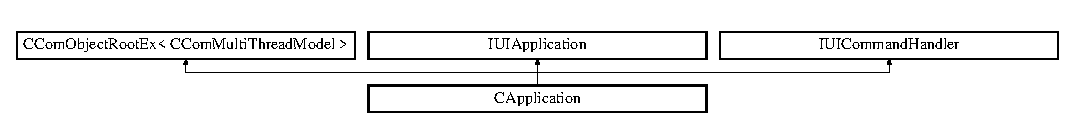
\includegraphics[height=1.287356cm]{class_c_application}
\end{center}
\end{figure}
\subsection*{Public Member Functions}
\begin{DoxyCompactItemize}
\item 
\hypertarget{class_c_application_a0a72c98b2cd788fec19349908c40d483}{S\-T\-D\-M\-E\-T\-H\-O\-D() {\bfseries On\-View\-Changed} (U\-I\-N\-T32 n\-View\-I\-D, \-\_\-\-\_\-in U\-I\-\_\-\-V\-I\-E\-W\-T\-Y\-P\-E type\-I\-D, \-\_\-\-\_\-in I\-Unknown $\ast$p\-View, U\-I\-\_\-\-V\-I\-E\-W\-V\-E\-R\-B verb, I\-N\-T32 u\-Reason\-Code)}\label{class_c_application_a0a72c98b2cd788fec19349908c40d483}

\item 
\hypertarget{class_c_application_ae2a5531439ab4e84c8ef77bfc1dd04e7}{S\-T\-D\-M\-E\-T\-H\-O\-D() {\bfseries On\-Create\-U\-I\-Command} (U\-I\-N\-T32 n\-Cmd\-I\-D, \-\_\-\-\_\-in U\-I\-\_\-\-C\-O\-M\-M\-A\-N\-D\-T\-Y\-P\-E type\-I\-D, \-\_\-\-\_\-deref\-\_\-out I\-U\-I\-Command\-Handler $\ast$$\ast$pp\-Command\-Handler)}\label{class_c_application_ae2a5531439ab4e84c8ef77bfc1dd04e7}

\item 
\hypertarget{class_c_application_a19a9c7447fa3c547166d5d1d8c9308ac}{S\-T\-D\-M\-E\-T\-H\-O\-D() {\bfseries On\-Destroy\-U\-I\-Command} (U\-I\-N\-T32 command\-Id, \-\_\-\-\_\-in U\-I\-\_\-\-C\-O\-M\-M\-A\-N\-D\-T\-Y\-P\-E type\-I\-D, \-\_\-\-\_\-in\-\_\-opt I\-U\-I\-Command\-Handler $\ast$p\-Command\-Handler)}\label{class_c_application_a19a9c7447fa3c547166d5d1d8c9308ac}

\item 
\hypertarget{class_c_application_a5f5e7397c0c70f7fb24e25a2013d031f}{S\-T\-D\-M\-E\-T\-H\-O\-D\-I\-M\-P {\bfseries Execute} (U\-I\-N\-T n\-Cmd\-I\-D, U\-I\-\_\-\-E\-X\-E\-C\-U\-T\-I\-O\-N\-V\-E\-R\-B verb, \-\_\-\-\_\-in\-\_\-opt const P\-R\-O\-P\-E\-R\-T\-Y\-K\-E\-Y $\ast$key, \-\_\-\-\_\-in\-\_\-opt const P\-R\-O\-P\-V\-A\-R\-I\-A\-N\-T $\ast$ppropvar\-Value, \-\_\-\-\_\-in\-\_\-opt I\-U\-I\-Simple\-Property\-Set $\ast$p\-Command\-Execution\-Properties)}\label{class_c_application_a5f5e7397c0c70f7fb24e25a2013d031f}

\item 
\hypertarget{class_c_application_a6d5911a93c8f39c3e0316ba43dc6dc8f}{S\-T\-D\-M\-E\-T\-H\-O\-D\-I\-M\-P {\bfseries Update\-Property} (U\-I\-N\-T n\-Cmd\-I\-D, \-\_\-\-\_\-in R\-E\-F\-P\-R\-O\-P\-E\-R\-T\-Y\-K\-E\-Y key, \-\_\-\-\_\-in\-\_\-opt const P\-R\-O\-P\-V\-A\-R\-I\-A\-N\-T $\ast$ppropvar\-Current\-Value, \-\_\-\-\_\-out P\-R\-O\-P\-V\-A\-R\-I\-A\-N\-T $\ast$ppropvar\-New\-Value)}\label{class_c_application_a6d5911a93c8f39c3e0316ba43dc6dc8f}

\end{DoxyCompactItemize}


The documentation for this class was generated from the following file\-:\begin{DoxyCompactItemize}
\item 
F\-:/\-S\-V\-N/\-P\-O\-P\-Tools/Ribbon.\-cpp\end{DoxyCompactItemize}

\hypertarget{class_c_dialog_event_handler}{\section{C\-Dialog\-Event\-Handler Class Reference}
\label{class_c_dialog_event_handler}\index{C\-Dialog\-Event\-Handler@{C\-Dialog\-Event\-Handler}}
}
Inheritance diagram for C\-Dialog\-Event\-Handler\-:\begin{figure}[H]
\begin{center}
\leavevmode
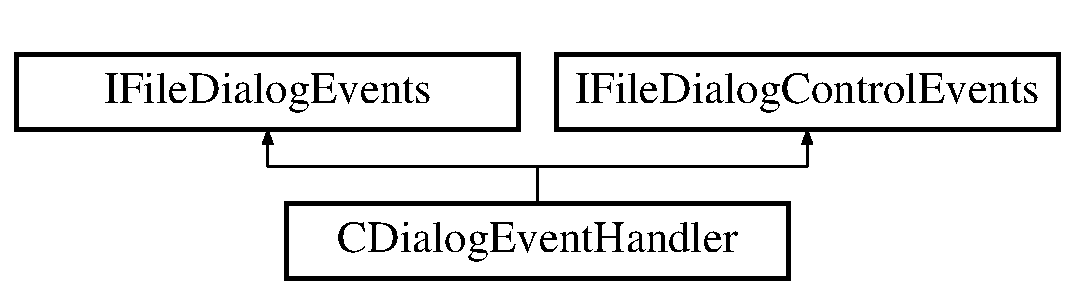
\includegraphics[height=2.000000cm]{class_c_dialog_event_handler}
\end{center}
\end{figure}
\subsection*{Public Member Functions}
\begin{DoxyCompactItemize}
\item 
\hypertarget{class_c_dialog_event_handler_a83da55cdef6e1160d6c8a0d613ca3bb5}{I\-F\-A\-C\-E\-M\-E\-T\-H\-O\-D\-I\-M\-P {\bfseries Query\-Interface} (R\-E\-F\-I\-I\-D riid, void $\ast$$\ast$ppv)}\label{class_c_dialog_event_handler_a83da55cdef6e1160d6c8a0d613ca3bb5}

\item 
\hypertarget{class_c_dialog_event_handler_a6f364e8217fa0170c12961e2129037f8}{{\bfseries I\-F\-A\-C\-E\-M\-E\-T\-H\-O\-D\-I\-M\-P\-\_\-} (U\-L\-O\-N\-G) Add\-Ref()}\label{class_c_dialog_event_handler_a6f364e8217fa0170c12961e2129037f8}

\item 
\hypertarget{class_c_dialog_event_handler_a529db231d24cf00bcd543e28bd134f1b}{{\bfseries I\-F\-A\-C\-E\-M\-E\-T\-H\-O\-D\-I\-M\-P\-\_\-} (U\-L\-O\-N\-G) Release()}\label{class_c_dialog_event_handler_a529db231d24cf00bcd543e28bd134f1b}

\item 
\hypertarget{class_c_dialog_event_handler_ad81cf46a3da3540100a9d5545be6aa12}{I\-F\-A\-C\-E\-M\-E\-T\-H\-O\-D\-I\-M\-P {\bfseries On\-File\-Ok} (I\-File\-Dialog $\ast$)}\label{class_c_dialog_event_handler_ad81cf46a3da3540100a9d5545be6aa12}

\item 
\hypertarget{class_c_dialog_event_handler_ac1be3a80796da8f129eceb373bdca2a7}{I\-F\-A\-C\-E\-M\-E\-T\-H\-O\-D\-I\-M\-P {\bfseries On\-Folder\-Change} (I\-File\-Dialog $\ast$)}\label{class_c_dialog_event_handler_ac1be3a80796da8f129eceb373bdca2a7}

\item 
\hypertarget{class_c_dialog_event_handler_ac8f0dd067b1a96f311bed4db0488788f}{I\-F\-A\-C\-E\-M\-E\-T\-H\-O\-D\-I\-M\-P {\bfseries On\-Folder\-Changing} (I\-File\-Dialog $\ast$, I\-Shell\-Item $\ast$)}\label{class_c_dialog_event_handler_ac8f0dd067b1a96f311bed4db0488788f}

\item 
\hypertarget{class_c_dialog_event_handler_aef6df46e375d52303619d97bca9fe57e}{I\-F\-A\-C\-E\-M\-E\-T\-H\-O\-D\-I\-M\-P {\bfseries On\-Help} (I\-File\-Dialog $\ast$)}\label{class_c_dialog_event_handler_aef6df46e375d52303619d97bca9fe57e}

\item 
\hypertarget{class_c_dialog_event_handler_ad1e341f5b5297c7b506d4b1e54a046cb}{I\-F\-A\-C\-E\-M\-E\-T\-H\-O\-D\-I\-M\-P {\bfseries On\-Selection\-Change} (I\-File\-Dialog $\ast$)}\label{class_c_dialog_event_handler_ad1e341f5b5297c7b506d4b1e54a046cb}

\item 
\hypertarget{class_c_dialog_event_handler_ae59130cbe514d9bb9faa9abaefcb91d8}{I\-F\-A\-C\-E\-M\-E\-T\-H\-O\-D\-I\-M\-P {\bfseries On\-Share\-Violation} (I\-File\-Dialog $\ast$, I\-Shell\-Item $\ast$, F\-D\-E\-\_\-\-S\-H\-A\-R\-E\-V\-I\-O\-L\-A\-T\-I\-O\-N\-\_\-\-R\-E\-S\-P\-O\-N\-S\-E $\ast$)}\label{class_c_dialog_event_handler_ae59130cbe514d9bb9faa9abaefcb91d8}

\item 
\hypertarget{class_c_dialog_event_handler_ac66c6e4a0e279074b8cc5a3fd786dc57}{I\-F\-A\-C\-E\-M\-E\-T\-H\-O\-D\-I\-M\-P {\bfseries On\-Type\-Change} (I\-File\-Dialog $\ast$pfd)}\label{class_c_dialog_event_handler_ac66c6e4a0e279074b8cc5a3fd786dc57}

\item 
\hypertarget{class_c_dialog_event_handler_a3bdc33d10116a6fc3d37b38a3843a1d5}{I\-F\-A\-C\-E\-M\-E\-T\-H\-O\-D\-I\-M\-P {\bfseries On\-Overwrite} (I\-File\-Dialog $\ast$, I\-Shell\-Item $\ast$, F\-D\-E\-\_\-\-O\-V\-E\-R\-W\-R\-I\-T\-E\-\_\-\-R\-E\-S\-P\-O\-N\-S\-E $\ast$)}\label{class_c_dialog_event_handler_a3bdc33d10116a6fc3d37b38a3843a1d5}

\item 
\hypertarget{class_c_dialog_event_handler_af3dd1df9281e0657adc7396dd0a419e1}{I\-F\-A\-C\-E\-M\-E\-T\-H\-O\-D\-I\-M\-P {\bfseries On\-Item\-Selected} (I\-File\-Dialog\-Customize $\ast$pfdc, D\-W\-O\-R\-D dw\-I\-D\-Ctl, D\-W\-O\-R\-D dw\-I\-D\-Item)}\label{class_c_dialog_event_handler_af3dd1df9281e0657adc7396dd0a419e1}

\item 
\hypertarget{class_c_dialog_event_handler_a88ab5f708ec246ab1fc4b766b0df1512}{I\-F\-A\-C\-E\-M\-E\-T\-H\-O\-D\-I\-M\-P {\bfseries On\-Button\-Clicked} (I\-File\-Dialog\-Customize $\ast$, D\-W\-O\-R\-D)}\label{class_c_dialog_event_handler_a88ab5f708ec246ab1fc4b766b0df1512}

\item 
\hypertarget{class_c_dialog_event_handler_a62f11342b7eb9b0f753033324eefc2f3}{I\-F\-A\-C\-E\-M\-E\-T\-H\-O\-D\-I\-M\-P {\bfseries On\-Check\-Button\-Toggled} (I\-File\-Dialog\-Customize $\ast$, D\-W\-O\-R\-D, B\-O\-O\-L)}\label{class_c_dialog_event_handler_a62f11342b7eb9b0f753033324eefc2f3}

\item 
\hypertarget{class_c_dialog_event_handler_a8c65afdb53848363c0c11f50aa15a92f}{I\-F\-A\-C\-E\-M\-E\-T\-H\-O\-D\-I\-M\-P {\bfseries On\-Control\-Activating} (I\-File\-Dialog\-Customize $\ast$, D\-W\-O\-R\-D)}\label{class_c_dialog_event_handler_a8c65afdb53848363c0c11f50aa15a92f}

\end{DoxyCompactItemize}


The documentation for this class was generated from the following file\-:\begin{DoxyCompactItemize}
\item 
F\-:/\-S\-V\-N/\-P\-O\-P\-Tools/Common\-File\-Dialog.\-cpp\end{DoxyCompactItemize}

\hypertarget{struct_compare_io_name}{\section{Compare\-Io\-Name$<$ T $>$ Struct Template Reference}
\label{struct_compare_io_name}\index{Compare\-Io\-Name$<$ T $>$@{Compare\-Io\-Name$<$ T $>$}}
}
Inheritance diagram for Compare\-Io\-Name$<$ T $>$\-:\begin{figure}[H]
\begin{center}
\leavevmode
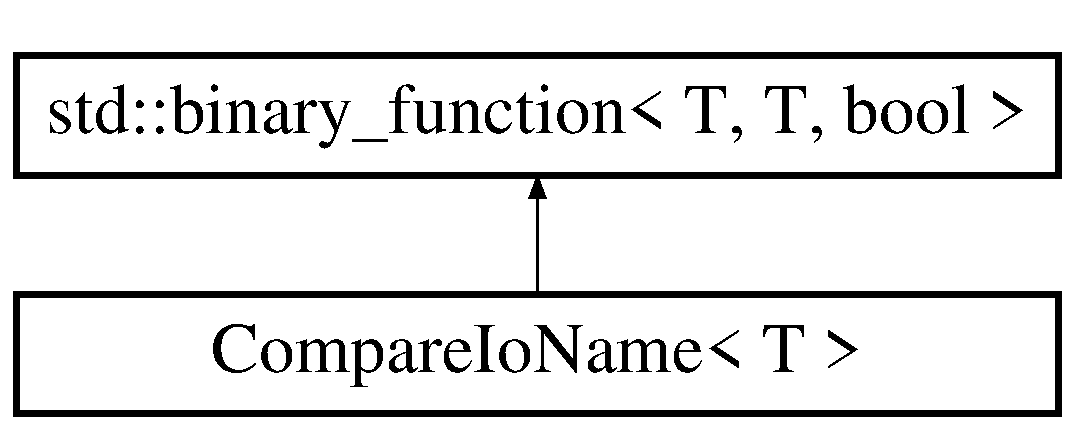
\includegraphics[height=2.000000cm]{struct_compare_io_name}
\end{center}
\end{figure}
\subsection*{Public Member Functions}
\begin{DoxyCompactItemize}
\item 
\hypertarget{struct_compare_io_name_ab9399673199623dac93109b3d8b68bd4}{bool {\bfseries operator()} (const T \&\-\_\-left, const T \&\-\_\-right)}\label{struct_compare_io_name_ab9399673199623dac93109b3d8b68bd4}

\end{DoxyCompactItemize}


The documentation for this struct was generated from the following file\-:\begin{DoxyCompactItemize}
\item 
F\-:/\-S\-V\-N/\-P\-O\-P\-Tools/iomap.\-cpp\end{DoxyCompactItemize}

\hypertarget{struct_compare_io_pin}{\section{Compare\-Io\-Pin$<$ T $>$ Struct Template Reference}
\label{struct_compare_io_pin}\index{Compare\-Io\-Pin$<$ T $>$@{Compare\-Io\-Pin$<$ T $>$}}
}
Inheritance diagram for Compare\-Io\-Pin$<$ T $>$\-:\begin{figure}[H]
\begin{center}
\leavevmode
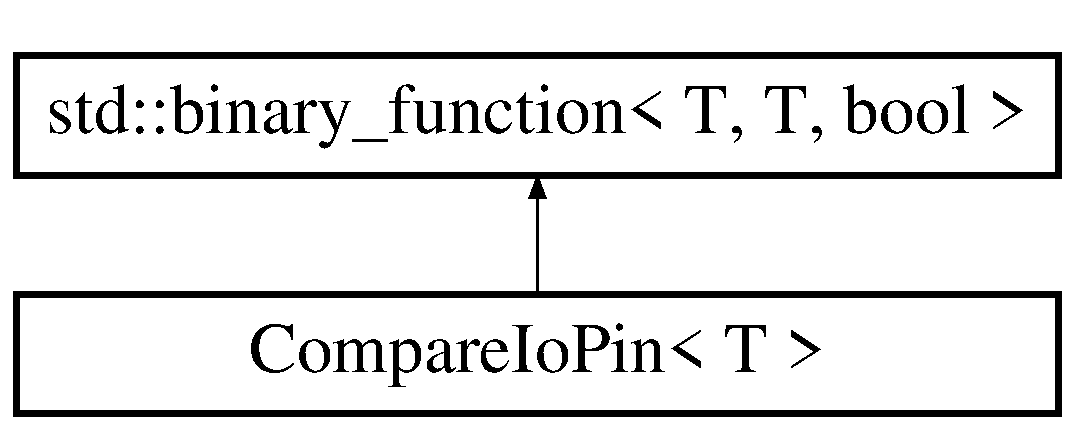
\includegraphics[height=2.000000cm]{struct_compare_io_pin}
\end{center}
\end{figure}
\subsection*{Public Member Functions}
\begin{DoxyCompactItemize}
\item 
\hypertarget{struct_compare_io_pin_a5a30503917f54843346f3b3916585384}{bool {\bfseries operator()} (const T \&\-\_\-left, const T \&\-\_\-right)}\label{struct_compare_io_pin_a5a30503917f54843346f3b3916585384}

\end{DoxyCompactItemize}


The documentation for this struct was generated from the following file\-:\begin{DoxyCompactItemize}
\item 
F\-:/\-S\-V\-N/\-P\-O\-P\-Tools/iomap.\-cpp\end{DoxyCompactItemize}

\hypertarget{struct_compare_io_port}{\section{Compare\-Io\-Port$<$ T $>$ Struct Template Reference}
\label{struct_compare_io_port}\index{Compare\-Io\-Port$<$ T $>$@{Compare\-Io\-Port$<$ T $>$}}
}
Inheritance diagram for Compare\-Io\-Port$<$ T $>$\-:\begin{figure}[H]
\begin{center}
\leavevmode
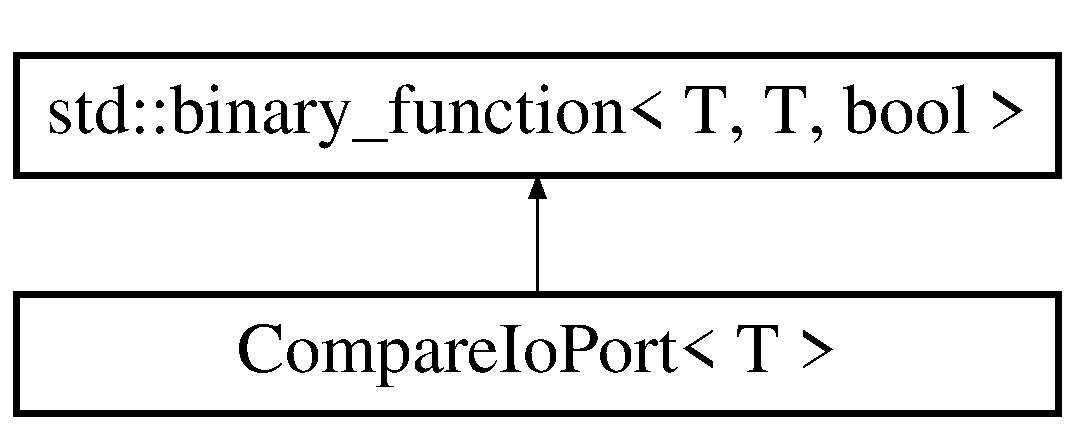
\includegraphics[height=2.000000cm]{struct_compare_io_port}
\end{center}
\end{figure}
\subsection*{Public Member Functions}
\begin{DoxyCompactItemize}
\item 
\hypertarget{struct_compare_io_port_af56b8177ac8b7d8faedfbd8e0a472b22}{bool {\bfseries operator()} (const T \&\-\_\-left, const T \&\-\_\-right)}\label{struct_compare_io_port_af56b8177ac8b7d8faedfbd8e0a472b22}

\end{DoxyCompactItemize}


The documentation for this struct was generated from the following file\-:\begin{DoxyCompactItemize}
\item 
F\-:/\-S\-V\-N/\-P\-O\-P\-Tools/iomap.\-cpp\end{DoxyCompactItemize}

\hypertarget{struct_compare_io_type}{\section{Compare\-Io\-Type$<$ T $>$ Struct Template Reference}
\label{struct_compare_io_type}\index{Compare\-Io\-Type$<$ T $>$@{Compare\-Io\-Type$<$ T $>$}}
}
Inheritance diagram for Compare\-Io\-Type$<$ T $>$\-:\begin{figure}[H]
\begin{center}
\leavevmode
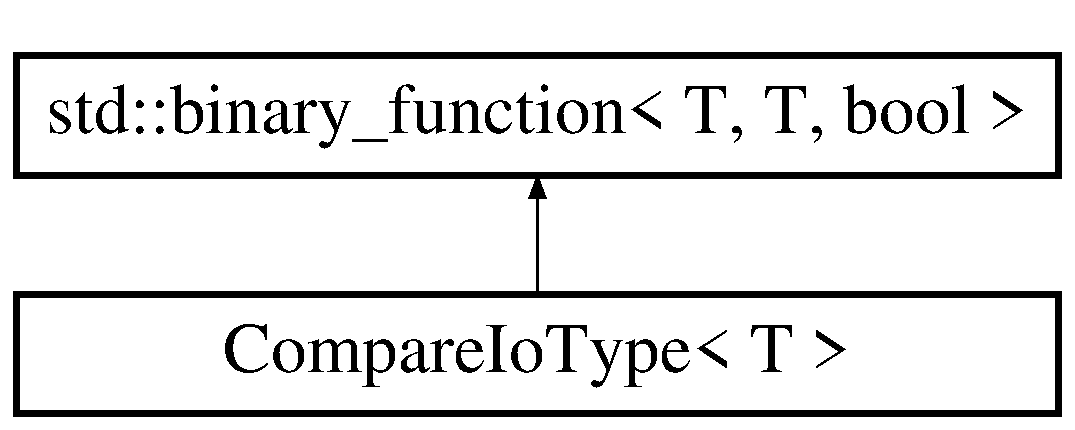
\includegraphics[height=2.000000cm]{struct_compare_io_type}
\end{center}
\end{figure}
\subsection*{Public Member Functions}
\begin{DoxyCompactItemize}
\item 
\hypertarget{struct_compare_io_type_a95f85774ed4337a060146495764d185c}{bool {\bfseries operator()} (const T \&\-\_\-left, const T \&\-\_\-right)}\label{struct_compare_io_type_a95f85774ed4337a060146495764d185c}

\end{DoxyCompactItemize}


The documentation for this struct was generated from the following file\-:\begin{DoxyCompactItemize}
\item 
F\-:/\-S\-V\-N/\-P\-O\-P\-Tools/iomap.\-cpp\end{DoxyCompactItemize}

\hypertarget{class_c_property_set}{\section{C\-Property\-Set Class Reference}
\label{class_c_property_set}\index{C\-Property\-Set@{C\-Property\-Set}}
}
Inheritance diagram for C\-Property\-Set\-:\begin{figure}[H]
\begin{center}
\leavevmode
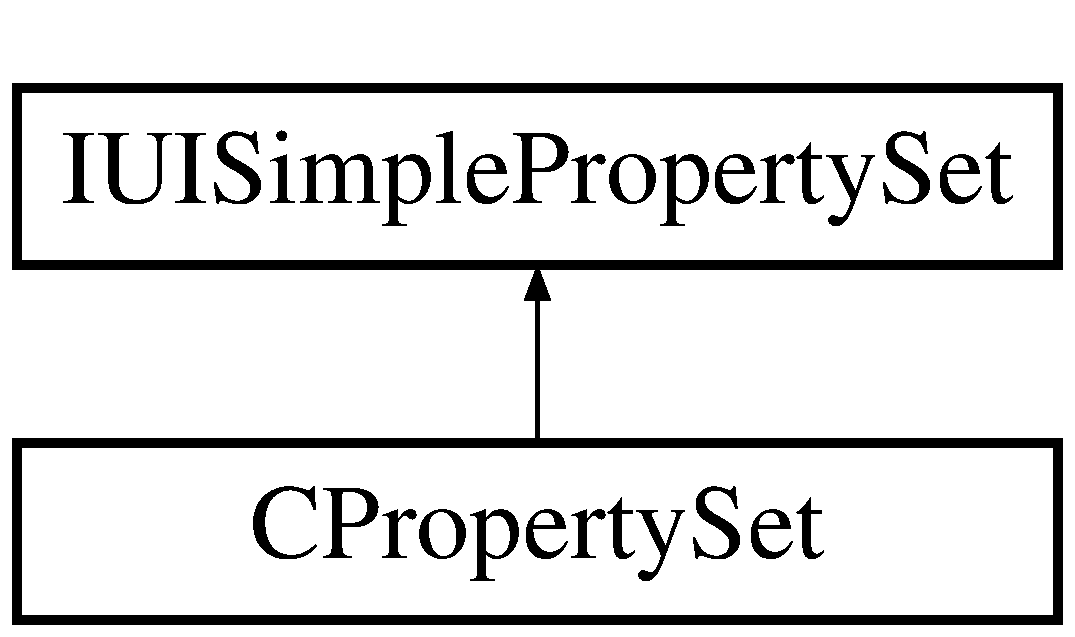
\includegraphics[height=2.000000cm]{class_c_property_set}
\end{center}
\end{figure}
\subsection*{Public Member Functions}
\begin{DoxyCompactItemize}
\item 
\hypertarget{class_c_property_set_a88e3aa4829e6f8a218488471382f2c0d}{void {\bfseries Initialize\-Command\-Properties} (int category\-Id, int command\-Id, U\-I\-\_\-\-C\-O\-M\-M\-A\-N\-D\-T\-Y\-P\-E command\-Type)}\label{class_c_property_set_a88e3aa4829e6f8a218488471382f2c0d}

\item 
\hypertarget{class_c_property_set_a3ec8e571945b29270d7eba5b653e18ac}{void {\bfseries Initialize\-Item\-Properties} (I\-U\-I\-Image $\ast$image, \-\_\-\-\_\-in P\-C\-W\-S\-T\-R label, int category\-Id)}\label{class_c_property_set_a3ec8e571945b29270d7eba5b653e18ac}

\item 
\hypertarget{class_c_property_set_a3eafcb9763909a26ab756d1028df83e4}{void {\bfseries Initialize\-Category\-Properties} (\-\_\-\-\_\-in P\-C\-W\-S\-T\-R label, int category\-Id)}\label{class_c_property_set_a3eafcb9763909a26ab756d1028df83e4}

\item 
\hypertarget{class_c_property_set_a56015a705d3c8137304a727be0de3b02}{S\-T\-D\-M\-E\-T\-H\-O\-D() {\bfseries Get\-Value} (\-\_\-\-\_\-in R\-E\-F\-P\-R\-O\-P\-E\-R\-T\-Y\-K\-E\-Y key, \-\_\-\-\_\-out P\-R\-O\-P\-V\-A\-R\-I\-A\-N\-T $\ast$ppropvar)}\label{class_c_property_set_a56015a705d3c8137304a727be0de3b02}

\item 
\hypertarget{class_c_property_set_a63033c80c286a1b29ee74429e3fe3769}{{\bfseries S\-T\-D\-M\-E\-T\-H\-O\-D\-\_\-} (U\-L\-O\-N\-G, Add\-Ref)()}\label{class_c_property_set_a63033c80c286a1b29ee74429e3fe3769}

\item 
\hypertarget{class_c_property_set_a719cb007f947586300699305ba95d0e7}{{\bfseries S\-T\-D\-M\-E\-T\-H\-O\-D\-\_\-} (U\-L\-O\-N\-G, Release)()}\label{class_c_property_set_a719cb007f947586300699305ba95d0e7}

\item 
\hypertarget{class_c_property_set_a4eec3cf79b6bfc761496bc162519770a}{S\-T\-D\-M\-E\-T\-H\-O\-D() {\bfseries Query\-Interface} (R\-E\-F\-I\-I\-D iid, void $\ast$$\ast$ppv)}\label{class_c_property_set_a4eec3cf79b6bfc761496bc162519770a}

\end{DoxyCompactItemize}
\subsection*{Static Public Member Functions}
\begin{DoxyCompactItemize}
\item 
\hypertarget{class_c_property_set_a7bba3def0c954a4fe0cff27f056a3607}{static H\-R\-E\-S\-U\-L\-T {\bfseries Create\-Instance} (\-\_\-\-\_\-deref\-\_\-out \hyperlink{class_c_property_set}{C\-Property\-Set} $\ast$$\ast$pp\-Property\-Set)}\label{class_c_property_set_a7bba3def0c954a4fe0cff27f056a3607}

\end{DoxyCompactItemize}


The documentation for this class was generated from the following files\-:\begin{DoxyCompactItemize}
\item 
F\-:/\-S\-V\-N/\-P\-O\-P\-Tools/Property\-Set.\-h\item 
F\-:/\-S\-V\-N/\-P\-O\-P\-Tools/Property\-Set.\-cpp\end{DoxyCompactItemize}

\hypertarget{class_c_recent_file_properties}{\section{C\-Recent\-File\-Properties Class Reference}
\label{class_c_recent_file_properties}\index{C\-Recent\-File\-Properties@{C\-Recent\-File\-Properties}}
}
Inheritance diagram for C\-Recent\-File\-Properties\-:\begin{figure}[H]
\begin{center}
\leavevmode
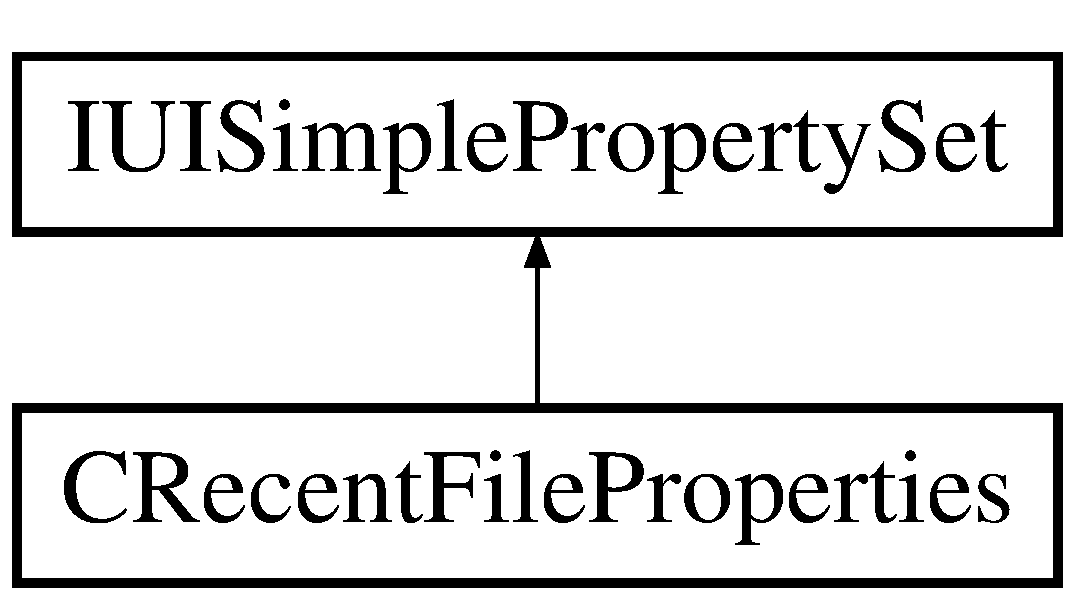
\includegraphics[height=2.000000cm]{class_c_recent_file_properties}
\end{center}
\end{figure}
\subsection*{Public Member Functions}
\begin{DoxyCompactItemize}
\item 
\hypertarget{class_c_recent_file_properties_a43759c5b80143c716b84e94b8c8ba506}{{\bfseries S\-T\-D\-M\-E\-T\-H\-O\-D\-I\-M\-P\-\_\-} (U\-L\-O\-N\-G) Add\-Ref()}\label{class_c_recent_file_properties_a43759c5b80143c716b84e94b8c8ba506}

\item 
\hypertarget{class_c_recent_file_properties_a7481206788cc45f96c09de409a0742a4}{{\bfseries S\-T\-D\-M\-E\-T\-H\-O\-D\-I\-M\-P\-\_\-} (U\-L\-O\-N\-G) Release()}\label{class_c_recent_file_properties_a7481206788cc45f96c09de409a0742a4}

\item 
\hypertarget{class_c_recent_file_properties_ae09c6b29c74e88f7e47eae3d74ebb84e}{S\-T\-D\-M\-E\-T\-H\-O\-D\-I\-M\-P {\bfseries Query\-Interface} (R\-E\-F\-I\-I\-D iid, void $\ast$$\ast$ppv)}\label{class_c_recent_file_properties_ae09c6b29c74e88f7e47eae3d74ebb84e}

\item 
\hypertarget{class_c_recent_file_properties_acfc60a7dbcd2813506045bd356903255}{S\-T\-D\-M\-E\-T\-H\-O\-D\-I\-M\-P {\bfseries Get\-Value} (\-\_\-\-\_\-in R\-E\-F\-P\-R\-O\-P\-E\-R\-T\-Y\-K\-E\-Y key, \-\_\-\-\_\-out P\-R\-O\-P\-V\-A\-R\-I\-A\-N\-T $\ast$value)}\label{class_c_recent_file_properties_acfc60a7dbcd2813506045bd356903255}

\end{DoxyCompactItemize}
\subsection*{Static Public Member Functions}
\begin{DoxyCompactItemize}
\item 
\hypertarget{class_c_recent_file_properties_a685d5156bd3104a3b20ae8f98fd9680e}{static \-\_\-\-\_\-check\-Return H\-R\-E\-S\-U\-L\-T {\bfseries Create\-Instance} (\-\_\-\-\_\-in P\-W\-S\-T\-R wsz\-Full\-Path, \-\_\-\-\_\-deref\-\_\-out\-\_\-opt \hyperlink{class_c_recent_file_properties}{C\-Recent\-File\-Properties} $\ast$$\ast$pp\-Properties)}\label{class_c_recent_file_properties_a685d5156bd3104a3b20ae8f98fd9680e}

\end{DoxyCompactItemize}


The documentation for this class was generated from the following file\-:\begin{DoxyCompactItemize}
\item 
F\-:/\-S\-V\-N/\-P\-O\-P\-Tools/Ribbon.\-cpp\end{DoxyCompactItemize}

\hypertarget{class_engine_g_u_i}{\section{Engine\-G\-U\-I Class Reference}
\label{class_engine_g_u_i}\index{Engine\-G\-U\-I@{Engine\-G\-U\-I}}
}
Inheritance diagram for Engine\-G\-U\-I\-:\begin{figure}[H]
\begin{center}
\leavevmode
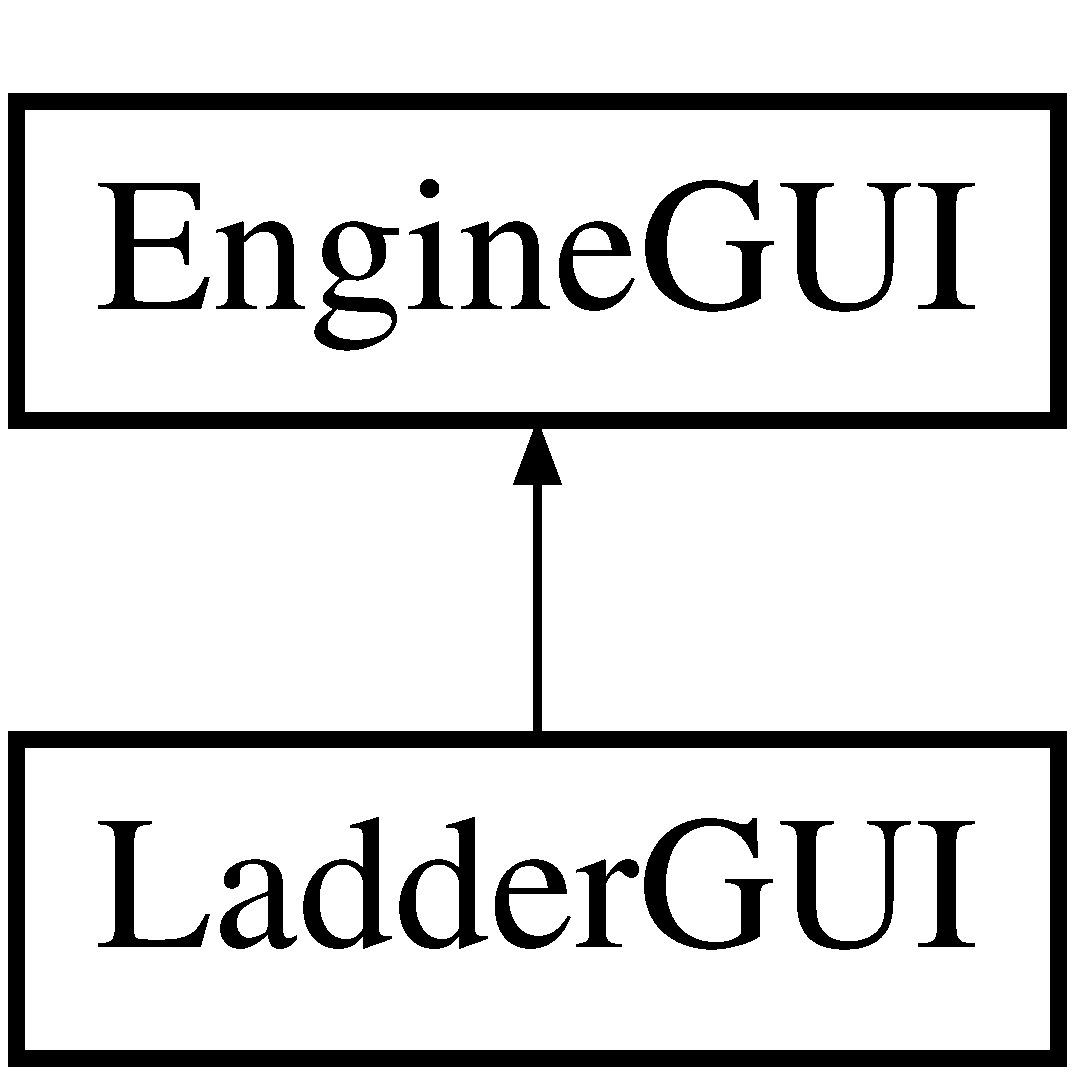
\includegraphics[height=2.000000cm]{class_engine_g_u_i}
\end{center}
\end{figure}
\subsection*{Public Member Functions}
\begin{DoxyCompactItemize}
\item 
\hypertarget{class_engine_g_u_i_adc0b7c5dcd7d4908aa2635cd6cf3c34f}{{\bfseries Engine\-G\-U\-I} (\hyperlink{class_engine_render}{Engine\-Render} $\ast$p\-R)}\label{class_engine_g_u_i_adc0b7c5dcd7d4908aa2635cd6cf3c34f}

\item 
\hypertarget{class_engine_g_u_i_aee68cba4eaa919df34766ac7868c1628}{{\bfseries Engine\-G\-U\-I} (\hyperlink{class_engine_render}{Engine\-Render} $\ast$p\-R, C\-O\-L\-O\-R\-R\-E\-F Background\-Color)}\label{class_engine_g_u_i_aee68cba4eaa919df34766ac7868c1628}

\item 
\hypertarget{class_engine_g_u_i_a3cbd4d4884317ba0d487d0b62d608ea9}{H\-R\-E\-S\-U\-L\-T {\bfseries Set\-Target} (H\-W\-N\-D hwnd)}\label{class_engine_g_u_i_a3cbd4d4884317ba0d487d0b62d608ea9}

\item 
\hypertarget{class_engine_g_u_i_aab6ce1cb30b93531f043b6ab16d1a77d}{H\-R\-E\-S\-U\-L\-T {\bfseries Set\-Render} (\hyperlink{class_engine_render}{Engine\-Render} $\ast$p\-R)}\label{class_engine_g_u_i_aab6ce1cb30b93531f043b6ab16d1a77d}

\item 
\hypertarget{class_engine_g_u_i_a0a50472d2e0852021f43cc3e7f323eab}{H\-R\-E\-S\-U\-L\-T {\bfseries Get\-Render} (\hyperlink{class_engine_render}{Engine\-Render} $\ast$$\ast$pp\-Render)}\label{class_engine_g_u_i_a0a50472d2e0852021f43cc3e7f323eab}

\item 
\hypertarget{class_engine_g_u_i_a568e73147bf0d0028862a5f5e322194b}{H\-R\-E\-S\-U\-L\-T {\bfseries Set\-Background\-Color} (C\-O\-L\-O\-R\-R\-E\-F rgb)}\label{class_engine_g_u_i_a568e73147bf0d0028862a5f5e322194b}

\item 
\hypertarget{class_engine_g_u_i_a91068b676bd6a30f309a8a57b1331efa}{unsigned int {\bfseries Create\-Brush} (C\-O\-L\-O\-R\-R\-E\-F rgb, float alpha=1.\-0f)}\label{class_engine_g_u_i_a91068b676bd6a30f309a8a57b1331efa}

\item 
\hypertarget{class_engine_g_u_i_a3a02a0f511e625781b9a9d647f2edcdb}{unsigned int {\bfseries Create\-Gradient} (unsigned int brush\-Start, unsigned int brush\-End, unsigned int angle=0)}\label{class_engine_g_u_i_a3a02a0f511e625781b9a9d647f2edcdb}

\item 
\hypertarget{class_engine_g_u_i_a98e705c23362e954755a7a9fb12d3b86}{P\-O\-I\-N\-T {\bfseries get\-Text\-Size} (const char $\ast$txt, P\-O\-I\-N\-T max\-Size, unsigned int format)}\label{class_engine_g_u_i_a98e705c23362e954755a7a9fb12d3b86}

\item 
\hypertarget{class_engine_g_u_i_a71abc09dfd4373f53a016b81d319b92b}{float {\bfseries get\-Brush\-Width} (void)}\label{class_engine_g_u_i_a71abc09dfd4373f53a016b81d319b92b}

\item 
\hypertarget{class_engine_g_u_i_aaa64bbc11cdf3ab5d5a636a1b1bf980e}{void {\bfseries set\-Brush\-Width} (float width)}\label{class_engine_g_u_i_aaa64bbc11cdf3ab5d5a636a1b1bf980e}

\item 
\hypertarget{class_engine_g_u_i_a5ce45d5f8bc98b30cccfd6d8fda686b1}{H\-R\-E\-S\-U\-L\-T {\bfseries Start\-Draw} (void)}\label{class_engine_g_u_i_a5ce45d5f8bc98b30cccfd6d8fda686b1}

\item 
\hypertarget{class_engine_g_u_i_a0cfff89732e8355a7e3ab25e7535fc58}{H\-R\-E\-S\-U\-L\-T {\bfseries Set\-Draw\-Offset} (P\-O\-I\-N\-T Offset)}\label{class_engine_g_u_i_a0cfff89732e8355a7e3ab25e7535fc58}

\item 
\hypertarget{class_engine_g_u_i_a8af860f8f34608642f032a3a9cd3765e}{H\-R\-E\-S\-U\-L\-T {\bfseries End\-Draw} (void)}\label{class_engine_g_u_i_a8af860f8f34608642f032a3a9cd3765e}

\item 
\hypertarget{class_engine_g_u_i_ae11c7743eeddb2db6cf9edf0f992118d}{H\-R\-E\-S\-U\-L\-T {\bfseries Draw\-Polygon} (vector$<$ P\-O\-I\-N\-T $>$ points, unsigned int brush, bool filled=true, unsigned int angle=0)}\label{class_engine_g_u_i_ae11c7743eeddb2db6cf9edf0f992118d}

\item 
\hypertarget{class_engine_g_u_i_a2cf65649bb05b1d2edd755a84bee8355}{H\-R\-E\-S\-U\-L\-T {\bfseries Draw\-Rectangle} (R\-E\-C\-T r, unsigned int brush, bool filled=true, unsigned int radius\-X=0, unsigned radius\-Y=0, unsigned int angle=0)}\label{class_engine_g_u_i_a2cf65649bb05b1d2edd755a84bee8355}

\item 
\hypertarget{class_engine_g_u_i_ab12a7539faa6a7ba9dcc50e007fba3d5}{H\-R\-E\-S\-U\-L\-T {\bfseries Draw\-Ellipse} (R\-E\-C\-T r, unsigned int brush, bool filled=true)}\label{class_engine_g_u_i_ab12a7539faa6a7ba9dcc50e007fba3d5}

\item 
\hypertarget{class_engine_g_u_i_aaf90583d3c91080a1a750e67805abdd7}{H\-R\-E\-S\-U\-L\-T {\bfseries Draw\-Ellipse} (P\-O\-I\-N\-T center, float rx, float ry, unsigned int brush, bool filled=true)}\label{class_engine_g_u_i_aaf90583d3c91080a1a750e67805abdd7}

\item 
\hypertarget{class_engine_g_u_i_aebe15c59ef2f1745d072f7d8b9bcb2b3}{H\-R\-E\-S\-U\-L\-T {\bfseries Draw\-Arc} (P\-O\-I\-N\-T start, P\-O\-I\-N\-T end, float rx, float ry, float angle, bool is\-Clock\-Wise, unsigned int brush)}\label{class_engine_g_u_i_aebe15c59ef2f1745d072f7d8b9bcb2b3}

\item 
\hypertarget{class_engine_g_u_i_a563e05f01065cde6c82e47a1eb4fdeea}{H\-R\-E\-S\-U\-L\-T {\bfseries Draw\-Text} (const char $\ast$txt, R\-E\-C\-T r, unsigned int format, unsigned int brush, e\-Align\-Mode align\-X, e\-Align\-Mode align\-Y, bool accept\-Multi\-Line=false)}\label{class_engine_g_u_i_a563e05f01065cde6c82e47a1eb4fdeea}

\item 
\hypertarget{class_engine_g_u_i_a9665be1816c3541751729fdc6b4c9528}{H\-R\-E\-S\-U\-L\-T {\bfseries Draw\-Line} (P\-O\-I\-N\-T start, P\-O\-I\-N\-T end, unsigned int brush, unsigned int angle=0)}\label{class_engine_g_u_i_a9665be1816c3541751729fdc6b4c9528}

\item 
\hypertarget{class_engine_g_u_i_a92c58187c0257ae4d9f54ab05152f9e9}{H\-R\-E\-S\-U\-L\-T {\bfseries Draw\-Picture\-From\-File} (char $\ast$filename, P\-O\-I\-N\-T start, P\-O\-I\-N\-T size)}\label{class_engine_g_u_i_a92c58187c0257ae4d9f54ab05152f9e9}

\item 
\hypertarget{class_engine_g_u_i_a34920930346eeffa575902894cd59130}{H\-R\-E\-S\-U\-L\-T {\bfseries Draw\-Picture\-From\-Resource} (int id, P\-O\-I\-N\-T start, P\-O\-I\-N\-T size)}\label{class_engine_g_u_i_a34920930346eeffa575902894cd59130}

\item 
\hypertarget{class_engine_g_u_i_ac3381c8e44d06325dc891a5a3b0cf2c2}{H\-R\-E\-S\-U\-L\-T {\bfseries Draw\-Rectangle3\-D} (R\-E\-C\-T r, float size\-Z, unsigned int brush\-B\-G, unsigned int brush\-Int\-Border, unsigned int brush\-Ext\-Border, bool filled=true, float radius\-X=20.\-0f, float radius\-Y=20.\-0f, float angle=0.\-0f)}\label{class_engine_g_u_i_ac3381c8e44d06325dc891a5a3b0cf2c2}

\end{DoxyCompactItemize}


The documentation for this class was generated from the following files\-:\begin{DoxyCompactItemize}
\item 
F\-:/\-S\-V\-N/\-P\-O\-P\-Tools/Engine\-G\-U\-I.\-h\item 
F\-:/\-S\-V\-N/\-P\-O\-P\-Tools/Engine\-G\-U\-I.\-cpp\end{DoxyCompactItemize}

\hypertarget{class_engine_render}{\section{Engine\-Render Class Reference}
\label{class_engine_render}\index{Engine\-Render@{Engine\-Render}}
}
Inheritance diagram for Engine\-Render\-:\begin{figure}[H]
\begin{center}
\leavevmode
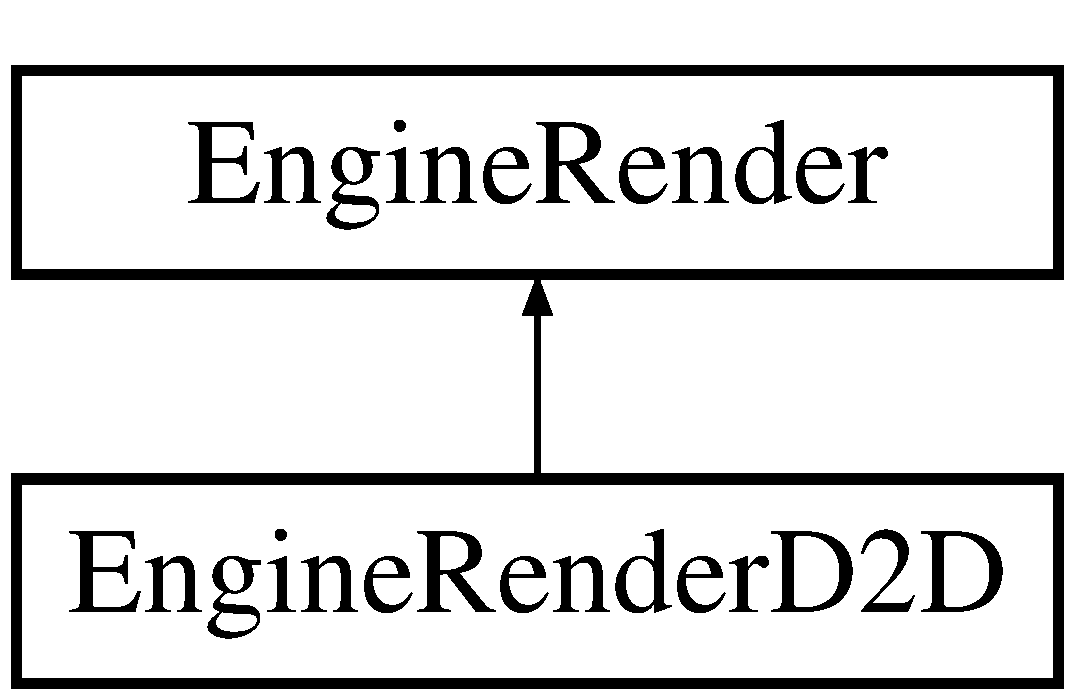
\includegraphics[height=2.000000cm]{class_engine_render}
\end{center}
\end{figure}
\subsection*{Public Member Functions}
\begin{DoxyCompactItemize}
\item 
\hypertarget{class_engine_render_a7b313144b67f23c97c1cf51912a56dc2}{virtual H\-R\-E\-S\-U\-L\-T {\bfseries Create\-Render\-Target} (H\-W\-N\-D hwnd)=0}\label{class_engine_render_a7b313144b67f23c97c1cf51912a56dc2}

\item 
\hypertarget{class_engine_render_abfb244fa8d5b2122d2b25b1dbef01020}{virtual H\-R\-E\-S\-U\-L\-T {\bfseries Resize\-Render\-Target} (H\-W\-N\-D hwnd)=0}\label{class_engine_render_abfb244fa8d5b2122d2b25b1dbef01020}

\item 
\hypertarget{class_engine_render_a6d381cafbf7934b4ffda51fdab4f0948}{virtual H\-R\-E\-S\-U\-L\-T {\bfseries Create\-Brush} (unsigned int \&index, unsigned int rgb, float alpha=1.\-0f)=0}\label{class_engine_render_a6d381cafbf7934b4ffda51fdab4f0948}

\item 
\hypertarget{class_engine_render_a55603101b883df3bfac84c54bd28bee4}{virtual H\-R\-E\-S\-U\-L\-T {\bfseries Create\-Gradient} (unsigned int \&index, unsigned int brush\-Start, unsigned int brush\-End, unsigned int angle=0)=0}\label{class_engine_render_a55603101b883df3bfac84c54bd28bee4}

\item 
\hypertarget{class_engine_render_a3d602eef3f305a65226fdbbda35d3a7d}{virtual P\-O\-I\-N\-T {\bfseries get\-Text\-Size} (const char $\ast$txt, P\-O\-I\-N\-T max\-Size, unsigned int format)=0}\label{class_engine_render_a3d602eef3f305a65226fdbbda35d3a7d}

\item 
\hypertarget{class_engine_render_a071a2b1f8ba2bc150c4e343d4c692b22}{virtual void {\bfseries Start\-Draw} (void)=0}\label{class_engine_render_a071a2b1f8ba2bc150c4e343d4c692b22}

\item 
\hypertarget{class_engine_render_ab79ea5186b14eaba38f62b440da15804}{virtual void {\bfseries Clear} (unsigned int brush)=0}\label{class_engine_render_ab79ea5186b14eaba38f62b440da15804}

\item 
\hypertarget{class_engine_render_ae925f3dc0627d4015ab1ae37e15d6db0}{virtual H\-R\-E\-S\-U\-L\-T {\bfseries End\-Draw} (void)=0}\label{class_engine_render_ae925f3dc0627d4015ab1ae37e15d6db0}

\item 
\hypertarget{class_engine_render_ae57893f1f5e300b15298d9aef667dd21}{virtual H\-R\-E\-S\-U\-L\-T {\bfseries Draw\-Polygon} (vector$<$ P\-O\-I\-N\-T $>$ points, unsigned int brush, bool filled=true, unsigned int angle=0, float brush\-Width=2.\-0f)=0}\label{class_engine_render_ae57893f1f5e300b15298d9aef667dd21}

\item 
\hypertarget{class_engine_render_a9e34edc812b813a2836f118276dc117e}{virtual void {\bfseries Draw\-Rectangle} (R\-E\-C\-T r, unsigned int brush, bool filled=true, unsigned int radius\-X=0, unsigned int radius\-Y=0, unsigned int angle=0, float brush\-Width=2.\-0f)=0}\label{class_engine_render_a9e34edc812b813a2836f118276dc117e}

\item 
\hypertarget{class_engine_render_a154177a8860a56b0039ac61ba77448b2}{virtual H\-R\-E\-S\-U\-L\-T {\bfseries Draw\-Ellipse} (P\-O\-I\-N\-T center, float rx, float ry, unsigned int brush, bool filled=true, float brush\-Width=2.\-0f)=0}\label{class_engine_render_a154177a8860a56b0039ac61ba77448b2}

\item 
\hypertarget{class_engine_render_a8f07ced0811c148a75f8bb77fb748071}{virtual H\-R\-E\-S\-U\-L\-T {\bfseries Draw\-Arc} (P\-O\-I\-N\-T start, P\-O\-I\-N\-T end, float rx, float ry, float angle, bool is\-Clock\-Wise, unsigned int brush, float brush\-Width=2.\-0f)=0}\label{class_engine_render_a8f07ced0811c148a75f8bb77fb748071}

\item 
\hypertarget{class_engine_render_a688754eb145ef5263e7b2a5fe46c3b50}{virtual void {\bfseries Draw\-Text} (const char $\ast$txt, R\-E\-C\-T r, unsigned int format, unsigned int brush, e\-Align\-Mode align\-X, e\-Align\-Mode align\-Y, bool accept\-Multi\-Line=false)=0}\label{class_engine_render_a688754eb145ef5263e7b2a5fe46c3b50}

\item 
\hypertarget{class_engine_render_a06012d41e9f0d9d46718ed1a2b8fa779}{virtual H\-R\-E\-S\-U\-L\-T {\bfseries Draw\-Line} (P\-O\-I\-N\-T start, P\-O\-I\-N\-T end, unsigned int brush, unsigned int angle=0, float brush\-Width=2.\-0f)=0}\label{class_engine_render_a06012d41e9f0d9d46718ed1a2b8fa779}

\item 
\hypertarget{class_engine_render_a1261a3ce472a2b93bd382ebd61be4983}{virtual H\-R\-E\-S\-U\-L\-T {\bfseries Draw\-Picture\-From\-File} (char $\ast$filename, P\-O\-I\-N\-T start, P\-O\-I\-N\-T size)=0}\label{class_engine_render_a1261a3ce472a2b93bd382ebd61be4983}

\item 
\hypertarget{class_engine_render_a16841455d17cccb27b468e2953d66083}{virtual H\-R\-E\-S\-U\-L\-T {\bfseries Draw\-Picture\-From\-Resource} (int id, P\-O\-I\-N\-T start, P\-O\-I\-N\-T size)=0}\label{class_engine_render_a16841455d17cccb27b468e2953d66083}

\item 
\hypertarget{class_engine_render_a22c73482820f4481e001d7167c5ab151}{virtual H\-R\-E\-S\-U\-L\-T {\bfseries Draw\-Rectangle3\-D} (R\-E\-C\-T r, float size\-Z, unsigned int brush\-B\-G, unsigned int brush\-Int\-Border, unsigned int brush\-Ext\-Border, bool filled=true, float radius\-X=20.\-0f, float radius\-Y=20.\-0f, float angle=0.\-0f)=0}\label{class_engine_render_a22c73482820f4481e001d7167c5ab151}

\end{DoxyCompactItemize}


The documentation for this class was generated from the following file\-:\begin{DoxyCompactItemize}
\item 
F\-:/\-S\-V\-N/\-P\-O\-P\-Tools/Engine\-Render.\-h\end{DoxyCompactItemize}

\hypertarget{class_engine_render_d2_d}{\section{Engine\-Render\-D2\-D Class Reference}
\label{class_engine_render_d2_d}\index{Engine\-Render\-D2\-D@{Engine\-Render\-D2\-D}}
}
Inheritance diagram for Engine\-Render\-D2\-D\-:\begin{figure}[H]
\begin{center}
\leavevmode
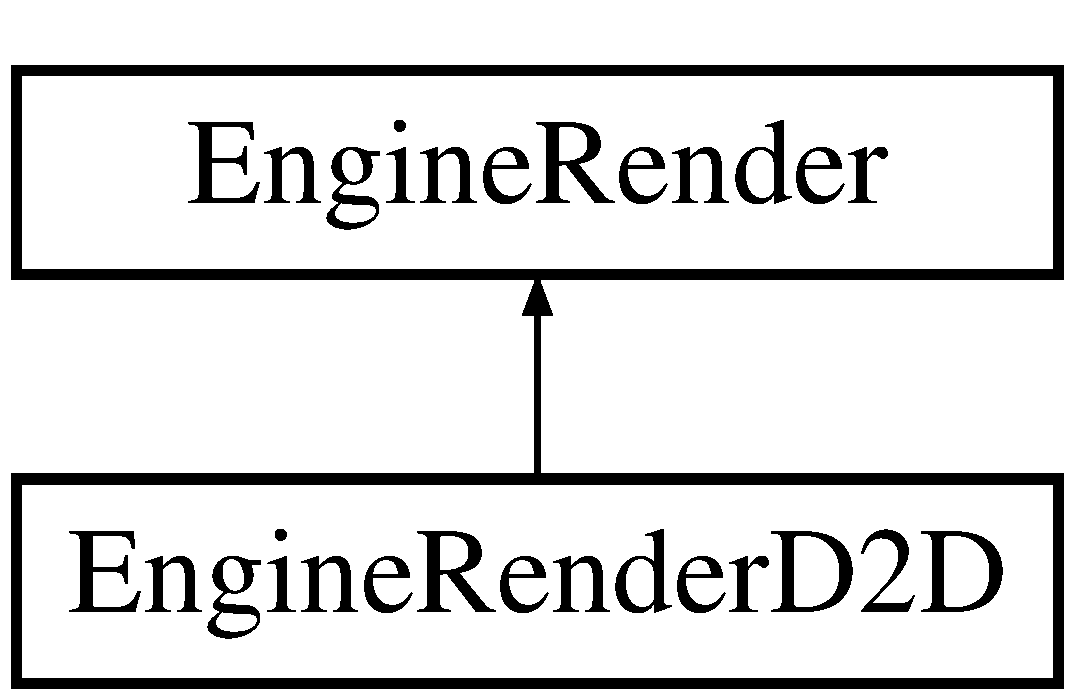
\includegraphics[height=2.000000cm]{class_engine_render_d2_d}
\end{center}
\end{figure}
\subsection*{Public Member Functions}
\begin{DoxyCompactItemize}
\item 
\hypertarget{class_engine_render_d2_d_a56684860134f55d48282e7f832b99025}{H\-R\-E\-S\-U\-L\-T {\bfseries Create\-Render\-Target} (H\-W\-N\-D hwnd)}\label{class_engine_render_d2_d_a56684860134f55d48282e7f832b99025}

\item 
\hypertarget{class_engine_render_d2_d_a2397760c24922853f424fcdfbcdeca5f}{H\-R\-E\-S\-U\-L\-T {\bfseries Resize\-Render\-Target} (H\-W\-N\-D hwnd)}\label{class_engine_render_d2_d_a2397760c24922853f424fcdfbcdeca5f}

\item 
\hypertarget{class_engine_render_d2_d_a2d1d72284ef7b0d2c1ca9ae7728b5baf}{H\-R\-E\-S\-U\-L\-T {\bfseries Create\-Brush} (unsigned int \&index, unsigned int rgb, float alpha=1.\-0f)}\label{class_engine_render_d2_d_a2d1d72284ef7b0d2c1ca9ae7728b5baf}

\item 
\hypertarget{class_engine_render_d2_d_adf5dbefc823835b11a825514ea0049d3}{H\-R\-E\-S\-U\-L\-T {\bfseries Create\-Gradient} (unsigned int \&index, unsigned int brush\-Start, unsigned int brush\-End, unsigned int angle=0)}\label{class_engine_render_d2_d_adf5dbefc823835b11a825514ea0049d3}

\item 
\hypertarget{class_engine_render_d2_d_a96bfcb4a434d7a48d71ddfb1d937c162}{H\-R\-E\-S\-U\-L\-T {\bfseries Create\-Text\-Format} (unsigned int rgb, unsigned int \&index)}\label{class_engine_render_d2_d_a96bfcb4a434d7a48d71ddfb1d937c162}

\item 
\hypertarget{class_engine_render_d2_d_a1099cab62b9fd79e17acdc68baab91b4}{P\-O\-I\-N\-T {\bfseries get\-Text\-Size} (const char $\ast$txt, P\-O\-I\-N\-T max\-Size, unsigned int format)}\label{class_engine_render_d2_d_a1099cab62b9fd79e17acdc68baab91b4}

\item 
\hypertarget{class_engine_render_d2_d_ac70574232e697bf3592cc65eb4ac8dc5}{I\-D2\-D1\-Brush $\ast$ {\bfseries get\-Brush} (unsigned int brush, D2\-D1\-\_\-\-R\-E\-C\-T\-\_\-\-F rf)}\label{class_engine_render_d2_d_ac70574232e697bf3592cc65eb4ac8dc5}

\item 
\hypertarget{class_engine_render_d2_d_a9be2d9733ba86d23cea5758d124bded9}{I\-D2\-D1\-Solid\-Color\-Brush $\ast$ {\bfseries get\-Solid\-Color\-Brush} (unsigned int brush)}\label{class_engine_render_d2_d_a9be2d9733ba86d23cea5758d124bded9}

\item 
\hypertarget{class_engine_render_d2_d_ac0df98ea121f6aabcfa043f19c983b32}{I\-D2\-D1\-Linear\-Gradient\-Brush $\ast$ {\bfseries get\-Linear\-Gradient\-Brush} (unsigned int brush, D2\-D1\-\_\-\-R\-E\-C\-T\-\_\-\-F rf)}\label{class_engine_render_d2_d_ac0df98ea121f6aabcfa043f19c983b32}

\item 
\hypertarget{class_engine_render_d2_d_ab0bf3bdaa14f39a02d28755f6cc75438}{void {\bfseries Start\-Draw} (void)}\label{class_engine_render_d2_d_ab0bf3bdaa14f39a02d28755f6cc75438}

\item 
\hypertarget{class_engine_render_d2_d_ab7e675bc41b33a614b2caf94f828c957}{void {\bfseries Clear} (unsigned int brush)}\label{class_engine_render_d2_d_ab7e675bc41b33a614b2caf94f828c957}

\item 
\hypertarget{class_engine_render_d2_d_a847ae770e8a4f4d054d5d4e336c4db62}{H\-R\-E\-S\-U\-L\-T {\bfseries End\-Draw} (void)}\label{class_engine_render_d2_d_a847ae770e8a4f4d054d5d4e336c4db62}

\item 
\hypertarget{class_engine_render_d2_d_a53738f7c724e5eef8ef953c31089241a}{H\-R\-E\-S\-U\-L\-T {\bfseries Draw\-Polygon} (vector$<$ P\-O\-I\-N\-T $>$ points, unsigned int brush, bool filled=true, unsigned int angle=0, float brush\-Width=2.\-0f)}\label{class_engine_render_d2_d_a53738f7c724e5eef8ef953c31089241a}

\item 
\hypertarget{class_engine_render_d2_d_abe84d7b4f643e9fec9cb3bc7d26e7c8d}{void {\bfseries Draw\-Rectangle} (R\-E\-C\-T r, unsigned int brush, bool filled=true, unsigned int radius\-X=0, unsigned int radius\-Y=0, unsigned int angle=0, float brush\-Width=2.\-0f)}\label{class_engine_render_d2_d_abe84d7b4f643e9fec9cb3bc7d26e7c8d}

\item 
\hypertarget{class_engine_render_d2_d_a724b48a6f1ecd1f9288513efb86200d5}{H\-R\-E\-S\-U\-L\-T {\bfseries Draw\-Ellipse} (P\-O\-I\-N\-T center, float rx, float ry, unsigned int brush, bool filled=true, float brush\-Width=2.\-0f)}\label{class_engine_render_d2_d_a724b48a6f1ecd1f9288513efb86200d5}

\item 
\hypertarget{class_engine_render_d2_d_a01eab9c4d19e537057429fa4422dc50b}{H\-R\-E\-S\-U\-L\-T {\bfseries Draw\-Arc} (P\-O\-I\-N\-T start, P\-O\-I\-N\-T end, float rx, float ry, float angle, bool is\-Clock\-Wise, unsigned int brush, float brush\-Width=2.\-0f)}\label{class_engine_render_d2_d_a01eab9c4d19e537057429fa4422dc50b}

\item 
\hypertarget{class_engine_render_d2_d_a3bf4daa2c3f0e5a1d426a7eaabd1351c}{void {\bfseries Draw\-Text} (const char $\ast$txt, R\-E\-C\-T r, unsigned int format, unsigned int brush, e\-Align\-Mode align\-X, e\-Align\-Mode align\-Y, bool accept\-Multi\-Line)}\label{class_engine_render_d2_d_a3bf4daa2c3f0e5a1d426a7eaabd1351c}

\item 
\hypertarget{class_engine_render_d2_d_ac380ee5c9c67c78c3e2aa8fce29c29e5}{H\-R\-E\-S\-U\-L\-T {\bfseries Draw\-Line} (P\-O\-I\-N\-T start, P\-O\-I\-N\-T end, unsigned int brush, unsigned int angle=0, float brush\-Width=2.\-0f)}\label{class_engine_render_d2_d_ac380ee5c9c67c78c3e2aa8fce29c29e5}

\item 
\hypertarget{class_engine_render_d2_d_adfd6dc6da9cdb4160ab718b9b5508c67}{H\-R\-E\-S\-U\-L\-T {\bfseries Draw\-Picture\-From\-File} (char $\ast$filename, P\-O\-I\-N\-T start, P\-O\-I\-N\-T size)}\label{class_engine_render_d2_d_adfd6dc6da9cdb4160ab718b9b5508c67}

\item 
\hypertarget{class_engine_render_d2_d_a097a7af4ad2ce1bf98738df5786b8265}{H\-R\-E\-S\-U\-L\-T {\bfseries Draw\-Picture\-From\-Resource} (int id, P\-O\-I\-N\-T start, P\-O\-I\-N\-T size)}\label{class_engine_render_d2_d_a097a7af4ad2ce1bf98738df5786b8265}

\item 
\hypertarget{class_engine_render_d2_d_a7add6bcd954002a40a47545833704099}{H\-R\-E\-S\-U\-L\-T {\bfseries Draw\-Rectangle3\-D} (R\-E\-C\-T r, float size\-Z, unsigned int brush\-B\-G, unsigned int brush\-Int\-Border, unsigned int brush\-Ext\-Border, bool filled, float radius\-X, float radius\-Y, float angle)}\label{class_engine_render_d2_d_a7add6bcd954002a40a47545833704099}

\end{DoxyCompactItemize}


The documentation for this class was generated from the following files\-:\begin{DoxyCompactItemize}
\item 
F\-:/\-S\-V\-N/\-P\-O\-P\-Tools/Engine\-Render\-D2\-D.\-h\item 
F\-:/\-S\-V\-N/\-P\-O\-P\-Tools/Engine\-Render\-D2\-D.\-cpp\end{DoxyCompactItemize}

\hypertarget{structfm__connectoptions__can}{\section{fm\-\_\-connectoptions\-\_\-can Struct Reference}
\label{structfm__connectoptions__can}\index{fm\-\_\-connectoptions\-\_\-can@{fm\-\_\-connectoptions\-\_\-can}}
}
\subsection*{Public Attributes}
\begin{DoxyCompactItemize}
\item 
\hypertarget{structfm__connectoptions__can_aab2a34800d6c9c5147a32978b9cf064e}{double {\bfseries osc}}\label{structfm__connectoptions__can_aab2a34800d6c9c5147a32978b9cf064e}

\item 
\hypertarget{structfm__connectoptions__can_a68f4164503ad9c78fd40d2558a62aa85}{int {\bfseries selecteddevice}}\label{structfm__connectoptions__can_a68f4164503ad9c78fd40d2558a62aa85}

\item 
\hypertarget{structfm__connectoptions__can_aedda769bcf313eb27a2b2aa9c0050da1}{int {\bfseries highspeed}}\label{structfm__connectoptions__can_aedda769bcf313eb27a2b2aa9c0050da1}

\item 
\hypertarget{structfm__connectoptions__can_adca85c7627d96ce661ffdc184cf4e1e6}{int {\bfseries interfacetype}}\label{structfm__connectoptions__can_adca85c7627d96ce661ffdc184cf4e1e6}

\item 
\hypertarget{structfm__connectoptions__can_a825eabcd2e80faa2033325b994f31579}{long {\bfseries baudrate}}\label{structfm__connectoptions__can_a825eabcd2e80faa2033325b994f31579}

\item 
\hypertarget{structfm__connectoptions__can_aa9403bc7331bab86e564ef6e6e4efaac}{unsigned long {\bfseries hwconfig} \mbox{[}2\mbox{]}}\label{structfm__connectoptions__can_aa9403bc7331bab86e564ef6e6e4efaac}

\item 
\hypertarget{structfm__connectoptions__can_ac618daf5113c5f04b098c208c0dba03c}{unsigned char {\bfseries nodeid}}\label{structfm__connectoptions__can_ac618daf5113c5f04b098c208c0dba03c}

\item 
\hypertarget{structfm__connectoptions__can_a34d62c8558a184115cd76b51e4faca8b}{long {\bfseries sdotimeout}}\label{structfm__connectoptions__can_a34d62c8558a184115cd76b51e4faca8b}

\end{DoxyCompactItemize}


The documentation for this struct was generated from the following file\-:\begin{DoxyCompactItemize}
\item 
F\-:/\-S\-V\-N/\-P\-O\-P\-Tools/flashmagiccommon.\-h\end{DoxyCompactItemize}

\hypertarget{structfm__connectoptions__com}{\section{fm\-\_\-connectoptions\-\_\-com Struct Reference}
\label{structfm__connectoptions__com}\index{fm\-\_\-connectoptions\-\_\-com@{fm\-\_\-connectoptions\-\_\-com}}
}
\subsection*{Public Attributes}
\begin{DoxyCompactItemize}
\item 
\hypertarget{structfm__connectoptions__com_ae4ba59f4626d01d6483df50c9fcd7d5c}{double {\bfseries osc}}\label{structfm__connectoptions__com_ae4ba59f4626d01d6483df50c9fcd7d5c}

\item 
\hypertarget{structfm__connectoptions__com_af558b743b914bae2232f1195f055ad2b}{int {\bfseries port}}\label{structfm__connectoptions__com_af558b743b914bae2232f1195f055ad2b}

\item 
\hypertarget{structfm__connectoptions__com_acef5c48fc2615a837e7ddfa27283eb99}{long {\bfseries baudrate}}\label{structfm__connectoptions__com_acef5c48fc2615a837e7ddfa27283eb99}

\item 
\hypertarget{structfm__connectoptions__com_abfa68faa25905e4883b42ad59dc98ca5}{int {\bfseries selecteddevice}}\label{structfm__connectoptions__com_abfa68faa25905e4883b42ad59dc98ca5}

\item 
\hypertarget{structfm__connectoptions__com_af82fa819fafc77eaa9318281cb6ccc30}{int {\bfseries highspeed}}\label{structfm__connectoptions__com_af82fa819fafc77eaa9318281cb6ccc30}

\item 
\hypertarget{structfm__connectoptions__com_a7b73b2439a6a7312515f2f1784fdeabf}{int {\bfseries clocks}}\label{structfm__connectoptions__com_a7b73b2439a6a7312515f2f1784fdeabf}

\item 
\hypertarget{structfm__connectoptions__com_a734d67e56f983056a9487c2a508d7b43}{int {\bfseries halfduplex}}\label{structfm__connectoptions__com_a734d67e56f983056a9487c2a508d7b43}

\item 
\hypertarget{structfm__connectoptions__com_aa2b51e5671dda35557c985cc27e186a6}{int {\bfseries hwconfig}}\label{structfm__connectoptions__com_aa2b51e5671dda35557c985cc27e186a6}

\item 
\hypertarget{structfm__connectoptions__com_a5f696ffc30512bf42c1febeb51d7f141}{int {\bfseries hwt1}}\label{structfm__connectoptions__com_a5f696ffc30512bf42c1febeb51d7f141}

\item 
\hypertarget{structfm__connectoptions__com_a3f80652eeca3d52e8d43560df9a85e27}{int {\bfseries hwt2}}\label{structfm__connectoptions__com_a3f80652eeca3d52e8d43560df9a85e27}

\item 
\hypertarget{structfm__connectoptions__com_a996217a59f2a6d1c0c3face3db4a73fd}{unsigned char {\bfseries i2caddr}}\label{structfm__connectoptions__com_a996217a59f2a6d1c0c3face3db4a73fd}

\item 
\hypertarget{structfm__connectoptions__com_afa88fe0975a941d9b252f3f27bc83cd1}{long {\bfseries maxbaudrate}}\label{structfm__connectoptions__com_afa88fe0975a941d9b252f3f27bc83cd1}

\item 
\hypertarget{structfm__connectoptions__com_a7bd912a3acca21681b9514928e29e3fc}{int {\bfseries usinginterface}}\label{structfm__connectoptions__com_a7bd912a3acca21681b9514928e29e3fc}

\item 
\hypertarget{structfm__connectoptions__com_a39cb5d63f9c8cf2bfce6f030f847eefb}{int {\bfseries interfacetype}}\label{structfm__connectoptions__com_a39cb5d63f9c8cf2bfce6f030f847eefb}

\end{DoxyCompactItemize}


The documentation for this struct was generated from the following file\-:\begin{DoxyCompactItemize}
\item 
F\-:/\-S\-V\-N/\-P\-O\-P\-Tools/flashmagiccommon.\-h\end{DoxyCompactItemize}

\hypertarget{structfm__connectoptions__ethernet}{\section{fm\-\_\-connectoptions\-\_\-ethernet Struct Reference}
\label{structfm__connectoptions__ethernet}\index{fm\-\_\-connectoptions\-\_\-ethernet@{fm\-\_\-connectoptions\-\_\-ethernet}}
}
\subsection*{Public Attributes}
\begin{DoxyCompactItemize}
\item 
\hypertarget{structfm__connectoptions__ethernet_ab6b5ac437af297d4473f720d197b88cc}{int {\bfseries adapterindex}}\label{structfm__connectoptions__ethernet_ab6b5ac437af297d4473f720d197b88cc}

\item 
\hypertarget{structfm__connectoptions__ethernet_a2fc154e52da6b39c0d1db0fcbc129c9f}{int {\bfseries selecteddevice}}\label{structfm__connectoptions__ethernet_a2fc154e52da6b39c0d1db0fcbc129c9f}

\item 
\hypertarget{structfm__connectoptions__ethernet_a292fb237173feb3ea06101ba2cd076ba}{unsigned long {\bfseries ipaddr}}\label{structfm__connectoptions__ethernet_a292fb237173feb3ea06101ba2cd076ba}

\item 
\hypertarget{structfm__connectoptions__ethernet_a8af0ac17e22a2833460bbcffe5a0c868}{unsigned char {\bfseries macaddr} \mbox{[}6\mbox{]}}\label{structfm__connectoptions__ethernet_a8af0ac17e22a2833460bbcffe5a0c868}

\end{DoxyCompactItemize}


The documentation for this struct was generated from the following file\-:\begin{DoxyCompactItemize}
\item 
F\-:/\-S\-V\-N/\-P\-O\-P\-Tools/flashmagiccommon.\-h\end{DoxyCompactItemize}

\hypertarget{structfm__results}{\section{fm\-\_\-results Struct Reference}
\label{structfm__results}\index{fm\-\_\-results@{fm\-\_\-results}}
}
\subsection*{Public Attributes}
\begin{DoxyCompactItemize}
\item 
\hypertarget{structfm__results_aa310a4cd9d65c40ffdf4e47592060479}{int {\bfseries result}}\label{structfm__results_aa310a4cd9d65c40ffdf4e47592060479}

\item 
\hypertarget{structfm__results_a62f9392c15760cabe0a59398e02c16b1}{unsigned char {\bfseries data} \mbox{[}F\-M\-\_\-\-M\-A\-X\-D\-A\-T\-A\-L\-E\-N\mbox{]}}\label{structfm__results_a62f9392c15760cabe0a59398e02c16b1}

\item 
\hypertarget{structfm__results_ad7fc604180eedd70d34e049e8c92576b}{char {\bfseries details} \mbox{[}F\-M\-\_\-\-M\-A\-X\-D\-E\-T\-A\-I\-L\-S\-L\-E\-N\mbox{]}}\label{structfm__results_ad7fc604180eedd70d34e049e8c92576b}

\end{DoxyCompactItemize}


The documentation for this struct was generated from the following file\-:\begin{DoxyCompactItemize}
\item 
F\-:/\-S\-V\-N/\-P\-O\-P\-Tools/flashmagiccommon.\-h\end{DoxyCompactItemize}

\hypertarget{struct_gallery_items}{\section{Gallery\-Items Struct Reference}
\label{struct_gallery_items}\index{Gallery\-Items@{Gallery\-Items}}
}
\subsection*{Public Attributes}
\begin{DoxyCompactItemize}
\item 
\hypertarget{struct_gallery_items_a03fb209bb15ac994d47a4ab31fb7efbf}{P\-C\-W\-S\-T\-R {\bfseries Cat\-Name}}\label{struct_gallery_items_a03fb209bb15ac994d47a4ab31fb7efbf}

\item 
\hypertarget{struct_gallery_items_a581003b5818ef5b1e49f4889da48e43c}{int {\bfseries List\-I\-D} \mbox{[}M\-A\-X\-\_\-\-I\-T\-E\-M\-S\mbox{]}}\label{struct_gallery_items_a581003b5818ef5b1e49f4889da48e43c}

\end{DoxyCompactItemize}


The documentation for this struct was generated from the following file\-:\begin{DoxyCompactItemize}
\item 
F\-:/\-S\-V\-N/\-P\-O\-P\-Tools/Ribbon.\-cpp\end{DoxyCompactItemize}

\hypertarget{struct_insertion_point}{\section{Insertion\-Point Struct Reference}
\label{struct_insertion_point}\index{Insertion\-Point@{Insertion\-Point}}
}
\subsection*{Public Attributes}
\begin{DoxyCompactItemize}
\item 
\hypertarget{struct_insertion_point_aa99d688ee66586eca63cc342d09a3108}{unsigned int {\bfseries point}}\label{struct_insertion_point_aa99d688ee66586eca63cc342d09a3108}

\item 
\hypertarget{struct_insertion_point_a5f2a724fc6bb6d13c2ece84d5e09c3d4}{\hyperlink{struct_subckt}{Subckt} {\bfseries subckt}}\label{struct_insertion_point_a5f2a724fc6bb6d13c2ece84d5e09c3d4}

\item 
\hypertarget{struct_insertion_point_a209dd4ba9be92b5dad1cab5cddda3763}{\hyperlink{class_ladder_circuit}{Ladder\-Circuit} $\ast$ {\bfseries series}}\label{struct_insertion_point_a209dd4ba9be92b5dad1cab5cddda3763}

\item 
\hypertarget{struct_insertion_point_ae8dae4baf6734111f448bcda10079219}{\hyperlink{class_ladder_circuit}{Ladder\-Circuit} $\ast$ {\bfseries parallel}}\label{struct_insertion_point_ae8dae4baf6734111f448bcda10079219}

\end{DoxyCompactItemize}


The documentation for this struct was generated from the following file\-:\begin{DoxyCompactItemize}
\item 
F\-:/\-S\-V\-N/\-P\-O\-P\-Tools/Ladder\-Objects.\-h\end{DoxyCompactItemize}

\hypertarget{class_int_code}{\section{Int\-Code Class Reference}
\label{class_int_code}\index{Int\-Code@{Int\-Code}}
}
\subsection*{Public Member Functions}
\begin{DoxyCompactItemize}
\item 
\hypertarget{class_int_code_a4fc3a7adfbcd7f2c06f3fa7fae990cae}{void {\bfseries Clear} (void)}\label{class_int_code_a4fc3a7adfbcd7f2c06f3fa7fae990cae}

\item 
\hypertarget{class_int_code_ae53945a620ab3d8e6f0db326a004efbe}{void {\bfseries Clear\-Parallel\-Count} (void)}\label{class_int_code_ae53945a620ab3d8e6f0db326a004efbe}

\item 
\hypertarget{class_int_code_a0d52b4b3dbd1df8ee96dfaffe5969ee7}{vector$<$ \hyperlink{struct_int_op_tag}{Int\-Op} $>$ {\bfseries get\-Vector\-Int\-Code} (void)}\label{class_int_code_a0d52b4b3dbd1df8ee96dfaffe5969ee7}

\item 
\hypertarget{class_int_code_a3de4afb7433741415b79185b63d2675c}{string {\bfseries Gen\-Sym\-Par\-This} (void)}\label{class_int_code_a3de4afb7433741415b79185b63d2675c}

\item 
\hypertarget{class_int_code_a86885d599550db8bf8dcdc48fd2ace37}{string {\bfseries Gen\-Sym\-Par\-Out} (void)}\label{class_int_code_a86885d599550db8bf8dcdc48fd2ace37}

\item 
\hypertarget{class_int_code_a6357a4a7e96c2795f00381f17282550c}{string {\bfseries Gen\-Sym\-One\-Shot} (void)}\label{class_int_code_a6357a4a7e96c2795f00381f17282550c}

\item 
\hypertarget{class_int_code_aeb4ddb87f783e660a41f9959ce2e644e}{string {\bfseries Gen\-Sym\-Formatted\-String} (void)}\label{class_int_code_aeb4ddb87f783e660a41f9959ce2e644e}

\item 
\hypertarget{class_int_code_a59c316ce6cc15a0ccf71ff4bc0e91c08}{int {\bfseries get\-Eeprom\-Addr} (void)}\label{class_int_code_a59c316ce6cc15a0ccf71ff4bc0e91c08}

\item 
\hypertarget{class_int_code_aadc8d6bef327519db6e730ddb2258182}{const char $\ast$ {\bfseries get\-State\-In\-Out} (void)}\label{class_int_code_aadc8d6bef327519db6e730ddb2258182}

\item 
\hypertarget{class_int_code_a3e32666b47ffa3de4235d95bd0ec608c}{void {\bfseries set\-State\-In\-Out} (string s)}\label{class_int_code_a3e32666b47ffa3de4235d95bd0ec608c}

\item 
\hypertarget{class_int_code_a329460a4f2ed5b072d5914d117eec67e}{void {\bfseries Op} (int op, const char $\ast$name1, const char $\ast$name2, const char $\ast$name3, const char $\ast$name4, const char $\ast$name5, const char $\ast$name6, const char $\ast$name7, S\-W\-O\-R\-D lit, unsigned char bit)}\label{class_int_code_a329460a4f2ed5b072d5914d117eec67e}

\item 
\hypertarget{class_int_code_ae3abaf8cc0ff9cc4c845a853c14e23f9}{void {\bfseries Op} (int op, const char $\ast$name1, const char $\ast$name2, const char $\ast$name3, const char $\ast$name4, S\-W\-O\-R\-D lit, unsigned char bit)}\label{class_int_code_ae3abaf8cc0ff9cc4c845a853c14e23f9}

\item 
\hypertarget{class_int_code_a1821d60d6d20742a430d086dde8f2833}{void {\bfseries Op} (int op, const char $\ast$name1, const char $\ast$name2, const char $\ast$name3, S\-W\-O\-R\-D lit, unsigned char bit)}\label{class_int_code_a1821d60d6d20742a430d086dde8f2833}

\item 
\hypertarget{class_int_code_a8644934876d977adde6e87c5c6f86206}{void {\bfseries Op} (int op, const char $\ast$name1, const char $\ast$name2, S\-W\-O\-R\-D lit)}\label{class_int_code_a8644934876d977adde6e87c5c6f86206}

\item 
\hypertarget{class_int_code_aff9baee761e162b15a2dd77d92c18b7b}{void {\bfseries Op} (int op, const char $\ast$name1, S\-W\-O\-R\-D lit)}\label{class_int_code_aff9baee761e162b15a2dd77d92c18b7b}

\item 
\hypertarget{class_int_code_abf95939f2a54c9dd874fbc03e23d48e8}{void {\bfseries Op} (int op, const char $\ast$name1, const char $\ast$name2)}\label{class_int_code_abf95939f2a54c9dd874fbc03e23d48e8}

\item 
\hypertarget{class_int_code_ae0db8fcdbbf5df8443fdcd68295a7bb4}{void {\bfseries Op} (int op, const char $\ast$name1)}\label{class_int_code_ae0db8fcdbbf5df8443fdcd68295a7bb4}

\item 
\hypertarget{class_int_code_ac04981db37dbfd163da285fbf9825f12}{void {\bfseries Op\-Bit} (int op, const char $\ast$name1, unsigned char bit)}\label{class_int_code_ac04981db37dbfd163da285fbf9825f12}

\item 
\hypertarget{class_int_code_aa85f465bf00e616b9e172eb9c64f4bf9}{void {\bfseries Op\-Bit} (int op, const char $\ast$name1, const char $\ast$name2, unsigned char bit)}\label{class_int_code_aa85f465bf00e616b9e172eb9c64f4bf9}

\item 
\hypertarget{class_int_code_ab725d3b310356fc944e54e620336ba75}{void {\bfseries Op} (int op)}\label{class_int_code_ab725d3b310356fc944e54e620336ba75}

\item 
\hypertarget{class_int_code_a717f5c98854f62bf945ab2baf80e7879}{void {\bfseries Sim\-State} (bool $\ast$b, const char $\ast$name)}\label{class_int_code_a717f5c98854f62bf945ab2baf80e7879}

\item 
\hypertarget{class_int_code_a1fe647104b3883d14d4f895f2313e914}{void {\bfseries Comment} (char $\ast$str,...)}\label{class_int_code_a1fe647104b3883d14d4f895f2313e914}

\item 
\hypertarget{class_int_code_a6dabd538b6b946015b048268ee857ff0}{const char $\ast$ {\bfseries Var\-From\-Expr} (const char $\ast$expr, char $\ast$temp\-Name)}\label{class_int_code_a6dabd538b6b946015b048268ee857ff0}

\end{DoxyCompactItemize}


The documentation for this class was generated from the following files\-:\begin{DoxyCompactItemize}
\item 
F\-:/\-S\-V\-N/\-P\-O\-P\-Tools/intcode.\-h\item 
F\-:/\-S\-V\-N/\-P\-O\-P\-Tools/intcode.\-cpp\end{DoxyCompactItemize}

\hypertarget{struct_int_op_tag}{\section{Int\-Op\-Tag Struct Reference}
\label{struct_int_op_tag}\index{Int\-Op\-Tag@{Int\-Op\-Tag}}
}
\subsection*{Public Attributes}
\begin{DoxyCompactItemize}
\item 
\hypertarget{struct_int_op_tag_a8fb14f9206116d7ab2399cfb29554278}{int {\bfseries op}}\label{struct_int_op_tag_a8fb14f9206116d7ab2399cfb29554278}

\item 
\hypertarget{struct_int_op_tag_a8f450f63bc63a7d2e378eace55c240bf}{char {\bfseries desc} \mbox{[}M\-A\-X\-\_\-\-N\-A\-M\-E\-\_\-\-L\-E\-N\mbox{]}}\label{struct_int_op_tag_a8f450f63bc63a7d2e378eace55c240bf}

\item 
\hypertarget{struct_int_op_tag_a56eba35f7963afa384fd717dca544d44}{char {\bfseries name1} \mbox{[}M\-A\-X\-\_\-\-N\-A\-M\-E\-\_\-\-L\-E\-N\mbox{]}}\label{struct_int_op_tag_a56eba35f7963afa384fd717dca544d44}

\item 
\hypertarget{struct_int_op_tag_ab20020d0b1bcfa3f9db63798ace3a28b}{char {\bfseries name2} \mbox{[}M\-A\-X\-\_\-\-N\-A\-M\-E\-\_\-\-L\-E\-N\mbox{]}}\label{struct_int_op_tag_ab20020d0b1bcfa3f9db63798ace3a28b}

\item 
\hypertarget{struct_int_op_tag_a113837fdacb56a5f3d1d463ae30a0cbf}{char {\bfseries name3} \mbox{[}M\-A\-X\-\_\-\-N\-A\-M\-E\-\_\-\-L\-E\-N\mbox{]}}\label{struct_int_op_tag_a113837fdacb56a5f3d1d463ae30a0cbf}

\item 
\hypertarget{struct_int_op_tag_ad2100e7f4c1f941febbf1bd507542351}{char {\bfseries name4} \mbox{[}M\-A\-X\-\_\-\-N\-A\-M\-E\-\_\-\-L\-E\-N\mbox{]}}\label{struct_int_op_tag_ad2100e7f4c1f941febbf1bd507542351}

\item 
\hypertarget{struct_int_op_tag_abde7fa039b9871c3714e6c07a607ec7f}{char {\bfseries name5} \mbox{[}M\-A\-X\-\_\-\-N\-A\-M\-E\-\_\-\-L\-E\-N\mbox{]}}\label{struct_int_op_tag_abde7fa039b9871c3714e6c07a607ec7f}

\item 
\hypertarget{struct_int_op_tag_a8549bc7df9ed51b131ac7624a83203a3}{char {\bfseries name6} \mbox{[}M\-A\-X\-\_\-\-N\-A\-M\-E\-\_\-\-L\-E\-N\mbox{]}}\label{struct_int_op_tag_a8549bc7df9ed51b131ac7624a83203a3}

\item 
\hypertarget{struct_int_op_tag_aa2a5a0a5a2bfcebedaa9dd87b2254823}{char {\bfseries name7} \mbox{[}M\-A\-X\-\_\-\-N\-A\-M\-E\-\_\-\-L\-E\-N\mbox{]}}\label{struct_int_op_tag_aa2a5a0a5a2bfcebedaa9dd87b2254823}

\item 
\hypertarget{struct_int_op_tag_a7e410eca78990d2a2f3fd1e0f9865918}{S\-W\-O\-R\-D {\bfseries literal}}\label{struct_int_op_tag_a7e410eca78990d2a2f3fd1e0f9865918}

\item 
\hypertarget{struct_int_op_tag_a9ae875b15498254e610453381ffc00a1}{bool $\ast$ {\bfseries powered\-After}}\label{struct_int_op_tag_a9ae875b15498254e610453381ffc00a1}

\item 
\hypertarget{struct_int_op_tag_abdf4dc9631aea42dee6d8b6f740e489c}{unsigned char {\bfseries bit}}\label{struct_int_op_tag_abdf4dc9631aea42dee6d8b6f740e489c}

\end{DoxyCompactItemize}


The documentation for this struct was generated from the following file\-:\begin{DoxyCompactItemize}
\item 
F\-:/\-S\-V\-N/\-P\-O\-P\-Tools/intcode.\-h\end{DoxyCompactItemize}

\hypertarget{class_keyboard_map}{\section{Keyboard\-Map Class Reference}
\label{class_keyboard_map}\index{Keyboard\-Map@{Keyboard\-Map}}
}
\subsection*{Public Member Functions}
\begin{DoxyCompactItemize}
\item 
\hypertarget{class_keyboard_map_aaefaa573454aab1ab6c5d33254a07770}{void {\bfseries Clear\-Maps} (void)}\label{class_keyboard_map_aaefaa573454aab1ab6c5d33254a07770}

\item 
\hypertarget{class_keyboard_map_ab7e85dae16117a99357240e777cd1ed6}{void {\bfseries Add\-Key} (int i\-Key, int i\-Flags, int($\ast$p\-Fnc)(void $\ast$p\-User\-Data), void $\ast$p\-User\-Data)}\label{class_keyboard_map_ab7e85dae16117a99357240e777cd1ed6}

\item 
\hypertarget{class_keyboard_map_aaf60f8316097101b7e48fc6f2aa90a14}{void {\bfseries Create\-Map} (int i\-Map\-I\-D)}\label{class_keyboard_map_aaf60f8316097101b7e48fc6f2aa90a14}

\item 
\hypertarget{class_keyboard_map_ac2f3a764de1cd597aec8f099afdcc123}{int {\bfseries Execute} (int i\-Key)}\label{class_keyboard_map_ac2f3a764de1cd597aec8f099afdcc123}

\item 
\hypertarget{class_keyboard_map_a07af1aea275ae7c373ef19fc6df4ea14}{void {\bfseries Set\-Map} (int i\-Map\-I\-D)}\label{class_keyboard_map_a07af1aea275ae7c373ef19fc6df4ea14}

\end{DoxyCompactItemize}


The documentation for this class was generated from the following files\-:\begin{DoxyCompactItemize}
\item 
F\-:/\-S\-V\-N/\-P\-O\-P\-Tools/Keyboard\-Map.\-h\item 
F\-:/\-S\-V\-N/\-P\-O\-P\-Tools/Keyboard\-Map.\-cpp\end{DoxyCompactItemize}

\hypertarget{class_ladder_circuit}{\section{Ladder\-Circuit Class Reference}
\label{class_ladder_circuit}\index{Ladder\-Circuit@{Ladder\-Circuit}}
}
\subsection*{Public Member Functions}
\begin{DoxyCompactItemize}
\item 
\hypertarget{class_ladder_circuit_a591845a7627d6dc4da984a7e5a54e825}{{\bfseries Ladder\-Circuit} (bool new\-Series)}\label{class_ladder_circuit_a591845a7627d6dc4da984a7e5a54e825}

\item 
\hypertarget{class_ladder_circuit_a902fb5573126a4386aca42f6309f5739}{bool {\bfseries Draw\-T\-X\-T} (vector$<$ vector$<$ int $>$ $>$ \&Display\-Matrix, int $\ast$cx, int $\ast$cy, bool powered\-Before, int Cols\-Available)}\label{class_ladder_circuit_a902fb5573126a4386aca42f6309f5739}

\item 
\hypertarget{class_ladder_circuit_a76d363c0d1b9f750a34603341e1984c8}{bool {\bfseries Draw\-G\-U\-I} (bool powered\-Before, void $\ast$data)}\label{class_ladder_circuit_a76d363c0d1b9f750a34603341e1984c8}

\item 
\hypertarget{class_ladder_circuit_afa7a478cef7e74d4ec31a9ff9f375383}{bool {\bfseries Is\-Comment} (void)}\label{class_ladder_circuit_afa7a478cef7e74d4ec31a9ff9f375383}

\item 
\hypertarget{class_ladder_circuit_ad7004fd97fd577d343327e725eabb020}{bool {\bfseries Is\-Empty} (void)}\label{class_ladder_circuit_ad7004fd97fd577d343327e725eabb020}

\item 
\hypertarget{class_ladder_circuit_adc0ba983b95ca7a8ebcc6faac7eecebb}{bool {\bfseries Is\-Last} (\hyperlink{class_ladder_elem}{Ladder\-Elem} $\ast$elem)}\label{class_ladder_circuit_adc0ba983b95ca7a8ebcc6faac7eecebb}

\item 
\hypertarget{class_ladder_circuit_a6c3512219be2441a30146e239d629d67}{bool {\bfseries Is\-Series} (void)}\label{class_ladder_circuit_a6c3512219be2441a30146e239d629d67}

\item 
\hypertarget{class_ladder_circuit_ac4c3691d11aa1d7964735325dc680bc9}{bool {\bfseries Has\-E\-O\-L} (void)}\label{class_ladder_circuit_ac4c3691d11aa1d7964735325dc680bc9}

\item 
\hypertarget{class_ladder_circuit_a42eeb7186c80bb5bdb76f3a356928b92}{bool {\bfseries Uart\-Function\-Used} (void)}\label{class_ladder_circuit_a42eeb7186c80bb5bdb76f3a356928b92}

\item 
\hypertarget{class_ladder_circuit_a517b76ad9fc6340c9bc189b1f84f016e}{bool {\bfseries Generate\-Int\-Code} (\hyperlink{class_int_code}{Int\-Code} \&ic)}\label{class_ladder_circuit_a517b76ad9fc6340c9bc189b1f84f016e}

\item 
\hypertarget{class_ladder_circuit_a8517d2327581a51eb0b5ce1ab90df0ff}{unsigned int {\bfseries get\-Size} (void)}\label{class_ladder_circuit_a8517d2327581a51eb0b5ce1ab90df0ff}

\item 
\hypertarget{class_ladder_circuit_a3b4b3aa4d5ecce70c6aa2bc3eae9268f}{\hyperlink{struct_subckt}{Subckt} {\bfseries get\-Next} (\hyperlink{struct_subckt}{Subckt} next)}\label{class_ladder_circuit_a3b4b3aa4d5ecce70c6aa2bc3eae9268f}

\item 
\hypertarget{class_ladder_circuit_aaf081a24dcba7fc641f4c1e085e4fe33}{\hyperlink{class_ladder_circuit}{Ladder\-Circuit} $\ast$ {\bfseries get\-Subckt\-For\-Element} (\hyperlink{class_ladder_elem}{Ladder\-Elem} $\ast$elem)}\label{class_ladder_circuit_aaf081a24dcba7fc641f4c1e085e4fe33}

\item 
\hypertarget{class_ladder_circuit_afeec19f4827ecf32e16b71f789f059cc}{\hyperlink{class_ladder_circuit}{Ladder\-Circuit} $\ast$ {\bfseries get\-Parent\-Subckt} (\hyperlink{class_ladder_circuit}{Ladder\-Circuit} $\ast$subckt)}\label{class_ladder_circuit_afeec19f4827ecf32e16b71f789f059cc}

\item 
\hypertarget{class_ladder_circuit_a3688d0ae1e57d25cd36245c481b24edd}{\hyperlink{struct_subckt}{Subckt} {\bfseries get\-Subckt} (unsigned int pos)}\label{class_ladder_circuit_a3688d0ae1e57d25cd36245c481b24edd}

\item 
\hypertarget{class_ladder_circuit_af10e56d2e4230337c7517eb9fb6e3287}{\hyperlink{class_ladder_elem}{Ladder\-Elem} $\ast$ {\bfseries get\-First\-Element} (void)}\label{class_ladder_circuit_af10e56d2e4230337c7517eb9fb6e3287}

\item 
\hypertarget{class_ladder_circuit_a97b709017e42e2650aab6ef296318eb4}{\hyperlink{class_ladder_elem}{Ladder\-Elem} $\ast$ {\bfseries get\-Last\-Element} (void)}\label{class_ladder_circuit_a97b709017e42e2650aab6ef296318eb4}

\item 
\hypertarget{class_ladder_circuit_ab3f5556c4a97dd2a113a7dae0f7a6246}{int {\bfseries get\-Width\-T\-X\-T} (int Cols\-Available)}\label{class_ladder_circuit_ab3f5556c4a97dd2a113a7dae0f7a6246}

\item 
\hypertarget{class_ladder_circuit_a725b879995b1805d40b5e02112792856}{int {\bfseries get\-Height\-T\-X\-T} (void)}\label{class_ladder_circuit_a725b879995b1805d40b5e02112792856}

\item 
\hypertarget{class_ladder_circuit_ae10bef7e261dc3891690412d0f99b91e}{void {\bfseries set\-Diagram} (\hyperlink{class_ladder_diagram}{Ladder\-Diagram} $\ast$new\-Diagram)}\label{class_ladder_circuit_ae10bef7e261dc3891690412d0f99b91e}

\item 
\hypertarget{class_ladder_circuit_ac3cf9ce530c2d950f4a1f7ecb56a46c6}{void {\bfseries Add\-Place\-Holder\-If\-No\-E\-O\-L} (\hyperlink{struct_ladder_context}{Ladder\-Context} context)}\label{class_ladder_circuit_ac3cf9ce530c2d950f4a1f7ecb56a46c6}

\item 
\hypertarget{class_ladder_circuit_ab118f0dec69df370e4b326a8fb2c72f0}{void {\bfseries Delete\-End\-Place\-Holder} (\hyperlink{struct_ladder_context}{Ladder\-Context} context)}\label{class_ladder_circuit_ab118f0dec69df370e4b326a8fb2c72f0}

\item 
\hypertarget{class_ladder_circuit_a4219e61d00df41af771227fbd93ad72f}{bool {\bfseries Add\-Element} (\hyperlink{class_ladder_elem}{Ladder\-Elem} $\ast$elem, \hyperlink{struct_ladder_context}{Ladder\-Context} \&context)}\label{class_ladder_circuit_a4219e61d00df41af771227fbd93ad72f}

\item 
\hypertarget{class_ladder_circuit_a55e9e35a6e8d2905bee5be1380edeb7f}{bool {\bfseries Insert\-Parallel} (\hyperlink{class_ladder_elem}{Ladder\-Elem} $\ast$elem, unsigned int start, unsigned int end, \hyperlink{struct_ladder_context}{Ladder\-Context} \&context)}\label{class_ladder_circuit_a55e9e35a6e8d2905bee5be1380edeb7f}

\item 
\hypertarget{class_ladder_circuit_a3e963fc9f837c240ca663b5bcdd383d7}{bool {\bfseries Del\-Element} (\hyperlink{class_ladder_elem}{Ladder\-Elem} $\ast$elem, \hyperlink{struct_ladder_context}{Ladder\-Context} \&context)}\label{class_ladder_circuit_a3e963fc9f837c240ca663b5bcdd383d7}

\item 
\hypertarget{class_ladder_circuit_ae71ff20b64d47d1a54769eb7229ac4f1}{void {\bfseries Remove\-Unnecessary\-Subckts} (\hyperlink{struct_ladder_context}{Ladder\-Context} context)}\label{class_ladder_circuit_ae71ff20b64d47d1a54769eb7229ac4f1}

\item 
\hypertarget{class_ladder_circuit_a435604093cdd1d6e35dfb0eb146a1b94}{int {\bfseries Search\-Match} (\hyperlink{class_ladder_circuit}{Ladder\-Circuit} $\ast$series, int direction)}\label{class_ladder_circuit_a435604093cdd1d6e35dfb0eb146a1b94}

\item 
\hypertarget{class_ladder_circuit_a96141987f7c71b37a7497f15d292c314}{int {\bfseries Elem\-In\-Subckt\-Series} (\hyperlink{struct_ladder_context}{Ladder\-Context} \&context, \hyperlink{struct_insertion_point}{Insertion\-Point} $\ast$point)}\label{class_ladder_circuit_a96141987f7c71b37a7497f15d292c314}

\item 
\hypertarget{class_ladder_circuit_a53aca622fef040ead057145de34cbc2e}{\hyperlink{class_ladder_circuit}{Ladder\-Circuit} $\ast$ {\bfseries Clone} (\hyperlink{class_ladder_diagram}{Ladder\-Diagram} $\ast$diagram)}\label{class_ladder_circuit_a53aca622fef040ead057145de34cbc2e}

\item 
\hypertarget{class_ladder_circuit_a5f55b0f2c276222b77c50d8dc9a14888}{void {\bfseries do\-Post\-Insert} (void)}\label{class_ladder_circuit_a5f55b0f2c276222b77c50d8dc9a14888}

\item 
\hypertarget{class_ladder_circuit_a34770fe88f488cd9311c63d3a36014ab}{void {\bfseries do\-Post\-Remove} (void)}\label{class_ladder_circuit_a34770fe88f488cd9311c63d3a36014ab}

\item 
\hypertarget{class_ladder_circuit_a880eba756722d65f571334ae740a2717}{bool {\bfseries Save} (\hyperlink{class_ladder_diagram}{Ladder\-Diagram} $\ast$diagram, F\-I\-L\-E $\ast$f)}\label{class_ladder_circuit_a880eba756722d65f571334ae740a2717}

\item 
\hypertarget{class_ladder_circuit_a904052549d1f10a052acdd064571fb8e}{bool {\bfseries Load} (\hyperlink{class_ladder_diagram}{Ladder\-Diagram} $\ast$diagram, F\-I\-L\-E $\ast$f, unsigned int version)}\label{class_ladder_circuit_a904052549d1f10a052acdd064571fb8e}

\item 
\hypertarget{class_ladder_circuit_aac89d1e01b7aae3e36fdc71604fc5d3e}{bool {\bfseries accept\-I\-O} (unsigned long id, e\-Type type)}\label{class_ladder_circuit_aac89d1e01b7aae3e36fdc71604fc5d3e}

\item 
\hypertarget{class_ladder_circuit_a6b7ef8c843b326323dd39acd434f8586}{void {\bfseries update\-I\-O} (\hyperlink{class_ladder_diagram}{Ladder\-Diagram} $\ast$owner, bool is\-Discard)}\label{class_ladder_circuit_a6b7ef8c843b326323dd39acd434f8586}

\item 
\hypertarget{class_ladder_circuit_a9cc949fe8e38a5328dfd97aa6df52353}{void {\bfseries get\-Allowed\-Types} (unsigned long id, vector$<$ e\-Type $>$ $\ast$types)}\label{class_ladder_circuit_a9cc949fe8e38a5328dfd97aa6df52353}

\item 
\hypertarget{class_ladder_circuit_a8b655379fb8cc962442613a13fa55a0d}{int {\bfseries Search\-And\-Replace} (\hyperlink{class_ladder_elem}{Ladder\-Elem} $\ast$$\ast$ref\-Elem, unsigned long id\-Search, string s\-New\-Text, e\-Search\-And\-Replace\-Mode mode)}\label{class_ladder_circuit_a8b655379fb8cc962442613a13fa55a0d}

\item 
\hypertarget{class_ladder_circuit_a61a5b7626cfb6c901ae2e486cee70814}{bool {\bfseries Do\-Undo\-Redo} (bool Is\-Undo, bool is\-Discard, \hyperlink{struct_undo_redo_action}{Undo\-Redo\-Action} \&action)}\label{class_ladder_circuit_a61a5b7626cfb6c901ae2e486cee70814}

\end{DoxyCompactItemize}
\subsection*{Protected Member Functions}
\begin{DoxyCompactItemize}
\item 
\hypertarget{class_ladder_circuit_a9b09244456b4a2de644c4d73f5577631}{bool {\bfseries Insert\-Subckt} (\hyperlink{struct_ladder_context}{Ladder\-Context} context, unsigned int pos, \hyperlink{struct_subckt}{Subckt} s, bool is\-Move=false, bool is\-Undo\-Redo=false)}\label{class_ladder_circuit_a9b09244456b4a2de644c4d73f5577631}

\item 
\hypertarget{class_ladder_circuit_a5641009934e13486aeae24153d7d5f83}{bool {\bfseries Delete\-Subckt} (\hyperlink{struct_ladder_context}{Ladder\-Context} context, unsigned int pos, bool is\-Move=false, bool is\-Undo\-Redo=false)}\label{class_ladder_circuit_a5641009934e13486aeae24153d7d5f83}

\item 
\hypertarget{class_ladder_circuit_a2e13373e5b67f22115de421711358292}{bool {\bfseries Move\-Subckt} (\hyperlink{struct_ladder_context}{Ladder\-Context} context, unsigned int pos, \hyperlink{class_ladder_circuit}{Ladder\-Circuit} $\ast$from\-Circuit, unsigned int from\-Pos, bool is\-Undo\-Redo=false)}\label{class_ladder_circuit_a2e13373e5b67f22115de421711358292}

\end{DoxyCompactItemize}


The documentation for this class was generated from the following files\-:\begin{DoxyCompactItemize}
\item 
F\-:/\-S\-V\-N/\-P\-O\-P\-Tools/Ladder\-Objects.\-h\item 
F\-:/\-S\-V\-N/\-P\-O\-P\-Tools/Ladder\-G\-U\-I.\-cpp\item 
F\-:/\-S\-V\-N/\-P\-O\-P\-Tools/Ladder\-Objects.\-cpp\end{DoxyCompactItemize}

\hypertarget{struct_ladder_clipboard}{\section{Ladder\-Clipboard Struct Reference}
\label{struct_ladder_clipboard}\index{Ladder\-Clipboard@{Ladder\-Clipboard}}
}
\subsection*{Public Attributes}
\begin{DoxyCompactItemize}
\item 
\hypertarget{struct_ladder_clipboard_ab60813407a49a93368fd6926e5306fed}{\hyperlink{class_ladder_elem}{Ladder\-Elem} $\ast$ {\bfseries elem\-Copy}}\label{struct_ladder_clipboard_ab60813407a49a93368fd6926e5306fed}

\item 
\hypertarget{struct_ladder_clipboard_a4ebbbd2a40a622cd6524191bdec6b546}{\hyperlink{class_ladder_diagram}{Ladder\-Diagram} $\ast$ {\bfseries elem\-Owner}}\label{struct_ladder_clipboard_a4ebbbd2a40a622cd6524191bdec6b546}

\item 
\hypertarget{struct_ladder_clipboard_af0bc660b4d995cf817a3f432b2851afb}{\hyperlink{struct_ladder_rung}{Ladder\-Rung} $\ast$ {\bfseries rung\-Copy}}\label{struct_ladder_clipboard_af0bc660b4d995cf817a3f432b2851afb}

\item 
\hypertarget{struct_ladder_clipboard_a1f9ffa748eefead4555624eba4025a60}{\hyperlink{class_ladder_diagram}{Ladder\-Diagram} $\ast$ {\bfseries rung\-Owner}}\label{struct_ladder_clipboard_a1f9ffa748eefead4555624eba4025a60}

\end{DoxyCompactItemize}


The documentation for this struct was generated from the following file\-:\begin{DoxyCompactItemize}
\item 
F\-:/\-S\-V\-N/\-P\-O\-P\-Tools/Ladder\-Objects.\-h\end{DoxyCompactItemize}

\hypertarget{struct_ladder_context}{\section{Ladder\-Context Struct Reference}
\label{struct_ladder_context}\index{Ladder\-Context@{Ladder\-Context}}
}
\subsection*{Public Attributes}
\begin{DoxyCompactItemize}
\item 
\hypertarget{struct_ladder_context_a0cd153c6cd68ec58538fe16aa755a4d7}{\hyperlink{class_ladder_elem}{Ladder\-Elem} $\ast$ {\bfseries Selected\-Elem}}\label{struct_ladder_context_a0cd153c6cd68ec58538fe16aa755a4d7}

\item 
\hypertarget{struct_ladder_context_adc0388c67ea4f9faf3763beab150bb66}{\hyperlink{class_ladder_elem}{Ladder\-Elem} $\ast$ {\bfseries Parallel\-Start}}\label{struct_ladder_context_adc0388c67ea4f9faf3763beab150bb66}

\item 
\hypertarget{struct_ladder_context_a8f47cac2d6a04a4f916ef7dfcc13d590}{\hyperlink{class_ladder_circuit}{Ladder\-Circuit} $\ast$ {\bfseries Selected\-Circuit}}\label{struct_ladder_context_a8f47cac2d6a04a4f916ef7dfcc13d590}

\item 
\hypertarget{struct_ladder_context_aa484b4d3e6dd32cc400bafd4fc27a938}{\hyperlink{class_ladder_diagram}{Ladder\-Diagram} $\ast$ {\bfseries Diagram}}\label{struct_ladder_context_aa484b4d3e6dd32cc400bafd4fc27a938}

\item 
\hypertarget{struct_ladder_context_ad9ba831337ff7b352ecb27b8452e5070}{int {\bfseries Selected\-State}}\label{struct_ladder_context_ad9ba831337ff7b352ecb27b8452e5070}

\item 
\hypertarget{struct_ladder_context_acbf5282e19ef9c23c8bea6ad291fff17}{bool {\bfseries in\-Simulation\-Mode}}\label{struct_ladder_context_acbf5282e19ef9c23c8bea6ad291fff17}

\item 
\hypertarget{struct_ladder_context_a2d0003249005a9f7b1237df6b930cbc8}{bool {\bfseries is\-Loading\-File}}\label{struct_ladder_context_a2d0003249005a9f7b1237df6b930cbc8}

\item 
\hypertarget{struct_ladder_context_ab833f4f179657323127ccba8a79f770f}{bool {\bfseries program\-Changed\-Not\-Saved}}\label{struct_ladder_context_ab833f4f179657323127ccba8a79f770f}

\item 
\hypertarget{struct_ladder_context_aecede7dbc285e32120548c687ee4754b}{bool {\bfseries can\-Negate}}\label{struct_ladder_context_aecede7dbc285e32120548c687ee4754b}

\item 
\hypertarget{struct_ladder_context_a4fd95b615aab13842309a6d78422618d}{bool {\bfseries can\-Normal}}\label{struct_ladder_context_a4fd95b615aab13842309a6d78422618d}

\item 
\hypertarget{struct_ladder_context_a61ba9d2b55247b59fec2851dbceff11d}{bool {\bfseries can\-Set\-Only}}\label{struct_ladder_context_a61ba9d2b55247b59fec2851dbceff11d}

\item 
\hypertarget{struct_ladder_context_aaeda31d47fbcfb8c144e71c5dcc721e6}{bool {\bfseries can\-Reset\-Only}}\label{struct_ladder_context_aaeda31d47fbcfb8c144e71c5dcc721e6}

\item 
\hypertarget{struct_ladder_context_af8729a23430774a03c7c4be3aaacad68}{bool {\bfseries can\-Push\-Up}}\label{struct_ladder_context_af8729a23430774a03c7c4be3aaacad68}

\item 
\hypertarget{struct_ladder_context_a340a738f533cb7e24180bbd762c57239}{bool {\bfseries can\-Push\-Down}}\label{struct_ladder_context_a340a738f533cb7e24180bbd762c57239}

\item 
\hypertarget{struct_ladder_context_a32ac15238228f4ede02f7b07c83eb83e}{bool {\bfseries can\-Delete}}\label{struct_ladder_context_a32ac15238228f4ede02f7b07c83eb83e}

\item 
\hypertarget{struct_ladder_context_ab8d097fa1a3afa4b24264e4b5f682bdc}{bool {\bfseries can\-Delete\-Rung}}\label{struct_ladder_context_ab8d097fa1a3afa4b24264e4b5f682bdc}

\item 
\hypertarget{struct_ladder_context_a430ac7b219ae5df9630a3cb98750b943}{bool {\bfseries can\-Insert\-End}}\label{struct_ladder_context_a430ac7b219ae5df9630a3cb98750b943}

\item 
\hypertarget{struct_ladder_context_a9f2ec64de0e09b8fa9478cca28c61708}{bool {\bfseries can\-Insert\-Other}}\label{struct_ladder_context_a9f2ec64de0e09b8fa9478cca28c61708}

\item 
\hypertarget{struct_ladder_context_aa86f43c59776db56278771b6fc3a1397}{bool {\bfseries can\-Insert\-Comment}}\label{struct_ladder_context_aa86f43c59776db56278771b6fc3a1397}

\end{DoxyCompactItemize}


The documentation for this struct was generated from the following file\-:\begin{DoxyCompactItemize}
\item 
F\-:/\-S\-V\-N/\-P\-O\-P\-Tools/Ladder\-Objects.\-h\end{DoxyCompactItemize}

\hypertarget{class_ladder_diagram}{\section{Ladder\-Diagram Class Reference}
\label{class_ladder_diagram}\index{Ladder\-Diagram@{Ladder\-Diagram}}
}
\subsection*{Public Member Functions}
\begin{DoxyCompactItemize}
\item 
\hypertarget{class_ladder_diagram_a5fac4c72b92f88e399226150aeba7c4e}{vector$<$ \hyperlink{struct_int_op_tag}{Int\-Op} $>$ {\bfseries get\-Vector\-Int\-Code} (void)}\label{class_ladder_diagram_a5fac4c72b92f88e399226150aeba7c4e}

\item 
\hypertarget{class_ladder_diagram_aa522b49a8548d31a97dd18813b00e54b}{bool {\bfseries Generate\-Int\-Code} (void)}\label{class_ladder_diagram_aa522b49a8548d31a97dd18813b00e54b}

\item 
\hypertarget{class_ladder_diagram_a1281eb6c4bd87936cdefd86aecbc869d}{int {\bfseries get\-Width\-T\-X\-T} (void)}\label{class_ladder_diagram_a1281eb6c4bd87936cdefd86aecbc869d}

\item 
\hypertarget{class_ladder_diagram_a17407fd1ac1bb69ed5ab426fb6289980}{int {\bfseries get\-Height\-T\-X\-T} (void)}\label{class_ladder_diagram_a17407fd1ac1bb69ed5ab426fb6289980}

\item 
\hypertarget{class_ladder_diagram_a1a54340c170a5b822704a306221b1b1b}{void {\bfseries update\-Context} (void)}\label{class_ladder_diagram_a1a54340c170a5b822704a306221b1b1b}

\item 
\hypertarget{class_ladder_diagram_acb86456fc1b93d7c9cbf6afab7055d1f}{\hyperlink{struct_ladder_context}{Ladder\-Context} {\bfseries get\-Context} (void)}\label{class_ladder_diagram_acb86456fc1b93d7c9cbf6afab7055d1f}

\item 
\hypertarget{class_ladder_diagram_af7adb162cbe87b329fc3b9d3f6d92632}{void {\bfseries Set\-Lock} (bool state)}\label{class_ladder_diagram_af7adb162cbe87b329fc3b9d3f6d92632}

\item 
\hypertarget{class_ladder_diagram_a74612b5a74cb7f21463c5fb789a07ada}{bool {\bfseries Is\-Locked} (void)}\label{class_ladder_diagram_a74612b5a74cb7f21463c5fb789a07ada}

\item 
\hypertarget{class_ladder_diagram_acfb0e7b5fb3ef36a1256c37dd88e7b28}{void {\bfseries Free\-Diagram} (void)}\label{class_ladder_diagram_acfb0e7b5fb3ef36a1256c37dd88e7b28}

\item 
\hypertarget{class_ladder_diagram_aec82ac7ac9e57612ee660bcb3174b147}{void {\bfseries Clear\-Diagram} (void)}\label{class_ladder_diagram_aec82ac7ac9e57612ee660bcb3174b147}

\item 
\hypertarget{class_ladder_diagram_a7821f02a13077d0b85d87481e251e869}{void {\bfseries New\-Diagram} (void)}\label{class_ladder_diagram_a7821f02a13077d0b85d87481e251e869}

\item 
\hypertarget{class_ladder_diagram_ae55ee99861de5acd7a5fb80ffaf89ef6}{void {\bfseries Activate} (bool is\-Active)}\label{class_ladder_diagram_ae55ee99861de5acd7a5fb80ffaf89ef6}

\item 
\hypertarget{class_ladder_diagram_a59dc32550ac5e29085b440e9f0798060}{void {\bfseries Select\-Element} (\hyperlink{class_ladder_elem}{Ladder\-Elem} $\ast$elem, int state)}\label{class_ladder_diagram_a59dc32550ac5e29085b440e9f0798060}

\item 
\hypertarget{class_ladder_diagram_ad03ae0f17edb1b582492370917721ef5}{bool {\bfseries Add\-Element} (\hyperlink{class_ladder_elem}{Ladder\-Elem} $\ast$elem)}\label{class_ladder_diagram_ad03ae0f17edb1b582492370917721ef5}

\item 
\hypertarget{class_ladder_diagram_ade22ce172477a8532c69e785238f8e40}{bool {\bfseries Del\-Element} (\hyperlink{class_ladder_elem}{Ladder\-Elem} $\ast$elem=nullptr)}\label{class_ladder_diagram_ade22ce172477a8532c69e785238f8e40}

\item 
\hypertarget{class_ladder_diagram_a3099b8c53d167759c5d0ca202e25f526}{bool {\bfseries Copy\-Element} (\hyperlink{struct_ladder_clipboard}{Ladder\-Clipboard} $\ast$clipboard, \hyperlink{class_ladder_elem}{Ladder\-Elem} $\ast$elem=nullptr)}\label{class_ladder_diagram_a3099b8c53d167759c5d0ca202e25f526}

\item 
\hypertarget{class_ladder_diagram_a4ea2aa6d914eaf440b996ce6f1e51764}{bool {\bfseries Paste\-Element} (\hyperlink{struct_ladder_clipboard}{Ladder\-Clipboard} clipboard)}\label{class_ladder_diagram_a4ea2aa6d914eaf440b996ce6f1e51764}

\item 
\hypertarget{class_ladder_diagram_a61a00bd5e550aa59f85b401120094f0e}{bool {\bfseries Edit\-Selected\-Element} (void)}\label{class_ladder_diagram_a61a00bd5e550aa59f85b401120094f0e}

\item 
\hypertarget{class_ladder_diagram_aef213a13bf9d7eaf778b5bfe76418974}{int {\bfseries Rung\-Containing\-Element} (\hyperlink{class_ladder_elem}{Ladder\-Elem} $\ast$elem)}\label{class_ladder_diagram_aef213a13bf9d7eaf778b5bfe76418974}

\item 
\hypertarget{class_ladder_diagram_a5c38ecbe315616be46ad1585f29fbe4d}{int {\bfseries Rung\-Containing\-Selected} (void)}\label{class_ladder_diagram_a5c38ecbe315616be46ad1585f29fbe4d}

\item 
\hypertarget{class_ladder_diagram_a70ba44a2817eb1de16a2a76ae35ebe7e}{void {\bfseries New\-Rung} (bool is\-After)}\label{class_ladder_diagram_a70ba44a2817eb1de16a2a76ae35ebe7e}

\item 
\hypertarget{class_ladder_diagram_a3bc782d74d99e72316c7b359fad53eb4}{bool {\bfseries Push\-Rung} (int rung, bool up)}\label{class_ladder_diagram_a3bc782d74d99e72316c7b359fad53eb4}

\item 
\hypertarget{class_ladder_diagram_a12bd1188b326ac796bddf37cc4c646c6}{bool {\bfseries Delete\-Rung} (int rung)}\label{class_ladder_diagram_a12bd1188b326ac796bddf37cc4c646c6}

\item 
\hypertarget{class_ladder_diagram_af8dacae346f30fb5a62f49e4a6d59200}{bool {\bfseries Is\-Rung\-Empty} (unsigned int n)}\label{class_ladder_diagram_af8dacae346f30fb5a62f49e4a6d59200}

\item 
\hypertarget{class_ladder_diagram_a135c7db7b98011cf10700c75fbd0f397}{bool {\bfseries Copy\-Rung} (\hyperlink{struct_ladder_clipboard}{Ladder\-Clipboard} $\ast$clipboard, \hyperlink{class_ladder_elem}{Ladder\-Elem} $\ast$elem=nullptr)}\label{class_ladder_diagram_a135c7db7b98011cf10700c75fbd0f397}

\item 
\hypertarget{class_ladder_diagram_a5529eff9bc9e0c97cf6c66c3dcbfc519}{bool {\bfseries Paste\-Rung} (\hyperlink{struct_ladder_clipboard}{Ladder\-Clipboard} clipboard, bool is\-After)}\label{class_ladder_diagram_a5529eff9bc9e0c97cf6c66c3dcbfc519}

\item 
\hypertarget{class_ladder_diagram_ae085b4dad746914f503109edd48e835e}{void {\bfseries Draw\-T\-X\-T} (int Offset\-X)}\label{class_ladder_diagram_ae085b4dad746914f503109edd48e835e}

\item 
\hypertarget{class_ladder_diagram_a76e40f92784b491b2878593d11a6468c}{void {\bfseries Draw\-G\-U\-I} (void)}\label{class_ladder_diagram_a76e40f92784b491b2878593d11a6468c}

\item 
\hypertarget{class_ladder_diagram_a8dacdd5e729b31e7b84c8f309c538630}{void {\bfseries Need\-Redraw} (bool is\-Full\-Redraw)}\label{class_ladder_diagram_a8dacdd5e729b31e7b84c8f309c538630}

\item 
\hypertarget{class_ladder_diagram_a8281cf6cb963920e4f33d8ab713e816a}{bool {\bfseries Is\-Element\-Visible} (\hyperlink{class_ladder_elem}{Ladder\-Elem} $\ast$elem, bool is\-Fully\-Visible=true)}\label{class_ladder_diagram_a8281cf6cb963920e4f33d8ab713e816a}

\item 
\hypertarget{class_ladder_diagram_ad759d7de6d21facde36097367d408a4a}{bool {\bfseries Is\-Selected\-Visible} (bool is\-Fully\-Visible=true)}\label{class_ladder_diagram_ad759d7de6d21facde36097367d408a4a}

\item 
\hypertarget{class_ladder_diagram_a42ff9c87ca2aa69b4cd5979183de87c3}{void {\bfseries Mouse\-Move} (int x, int y)}\label{class_ladder_diagram_a42ff9c87ca2aa69b4cd5979183de87c3}

\item 
\hypertarget{class_ladder_diagram_a668c9201eaec8017096c563152e98f37}{void {\bfseries Mouse\-Click} (int x, int y, bool is\-Down, bool is\-Double)}\label{class_ladder_diagram_a668c9201eaec8017096c563152e98f37}

\item 
\hypertarget{class_ladder_diagram_a68890a0c7dc63663b5c8354efeb63d76}{void {\bfseries Move\-Cursor} (e\-Move\-Cursor move\-To)}\label{class_ladder_diagram_a68890a0c7dc63663b5c8354efeb63d76}

\item 
\hypertarget{class_ladder_diagram_a233b99e6a7c7c593516991764c7e3c8d}{\hyperlink{class_ladder_elem}{Ladder\-Elem} $\ast$ {\bfseries Search\-Element} (e\-Move\-Cursor move\-To)}\label{class_ladder_diagram_a233b99e6a7c7c593516991764c7e3c8d}

\item 
\hypertarget{class_ladder_diagram_a61586c47c22ac18ad532a5696de5d5e9}{bool {\bfseries Add\-Parallel\-Start} (void)}\label{class_ladder_diagram_a61586c47c22ac18ad532a5696de5d5e9}

\item 
\hypertarget{class_ladder_diagram_afb387a8560a9c9c5d390087b95a6a541}{bool {\bfseries Save} (string filename, bool dont\-Save\-Filename=false)}\label{class_ladder_diagram_afb387a8560a9c9c5d390087b95a6a541}

\item 
\hypertarget{class_ladder_diagram_a482e5850f545f9bc4d0966321be78c03}{bool {\bfseries Load} (string filename)}\label{class_ladder_diagram_a482e5850f545f9bc4d0966321be78c03}

\item 
\hypertarget{class_ladder_diagram_a02c8eb2ff9cedfd023463a842e10c7fd}{string {\bfseries get\-Current\-Filename} (void)}\label{class_ladder_diagram_a02c8eb2ff9cedfd023463a842e10c7fd}

\item 
\hypertarget{class_ladder_diagram_a2e7cb76665821bce88e255b654303b71}{void {\bfseries Program\-Changed} (void)}\label{class_ladder_diagram_a2e7cb76665821bce88e255b654303b71}

\item 
\hypertarget{class_ladder_diagram_a53729a521a2ff88ae078c74e50ae6a82}{\hyperlink{struct_mcu_io_info_tag}{Mcu\-Io\-Info} $\ast$ {\bfseries get\-M\-C\-U} (void)}\label{class_ladder_diagram_a53729a521a2ff88ae078c74e50ae6a82}

\item 
\hypertarget{class_ladder_diagram_a6e2de735f45b6cd06813e6aa440a0627}{void {\bfseries Toggle\-Break\-Point} (unsigned int rung)}\label{class_ladder_diagram_a6e2de735f45b6cd06813e6aa440a0627}

\item 
\hypertarget{class_ladder_diagram_a2a759cbb91062e086641024f1c864193}{\hyperlink{struct_ladder_settings_general}{Ladder\-Settings\-General} {\bfseries get\-Settings\-General} (void)}\label{class_ladder_diagram_a2a759cbb91062e086641024f1c864193}

\item 
\hypertarget{class_ladder_diagram_a3f1f5e176d568db09ab2704947f2f6d0}{\hyperlink{struct_ladder_settings_u_a_r_t}{Ladder\-Settings\-U\-A\-R\-T} {\bfseries get\-Settings\-U\-A\-R\-T} (void)}\label{class_ladder_diagram_a3f1f5e176d568db09ab2704947f2f6d0}

\item 
\hypertarget{class_ladder_diagram_a6cb4a103ca3ffd125a0d6f354790bdb8}{\hyperlink{struct_ladder_settings_network}{Ladder\-Settings\-Network} {\bfseries get\-Settings\-Network} (void)}\label{class_ladder_diagram_a6cb4a103ca3ffd125a0d6f354790bdb8}

\item 
\hypertarget{class_ladder_diagram_ae4ea634df989511e59bc79026163216e}{\hyperlink{struct_ladder_settings_s_n_t_p}{Ladder\-Settings\-S\-N\-T\-P} {\bfseries get\-Settings\-S\-N\-T\-P} (void)}\label{class_ladder_diagram_ae4ea634df989511e59bc79026163216e}

\item 
\hypertarget{class_ladder_diagram_ace931be043f897501ed392c77d24c720}{\hyperlink{struct_ladder_settings_encoder_incremental}{Ladder\-Settings\-Encoder\-Incremental} {\bfseries get\-Settings\-Encoder\-Incremental} (void)}\label{class_ladder_diagram_ace931be043f897501ed392c77d24c720}

\item 
\hypertarget{class_ladder_diagram_a0fbd49c86820862eaf80703823abc7d6}{\hyperlink{struct_ladder_settings_encoder_s_s_i}{Ladder\-Settings\-Encoder\-S\-S\-I} {\bfseries get\-Settings\-Encoder\-S\-S\-I} (void)}\label{class_ladder_diagram_a0fbd49c86820862eaf80703823abc7d6}

\item 
\hypertarget{class_ladder_diagram_af9ef1953c10507a77b123a051477ae17}{\hyperlink{struct_ladder_settings_a_d_c}{Ladder\-Settings\-A\-D\-C} {\bfseries get\-Settings\-A\-D\-C} (void)}\label{class_ladder_diagram_af9ef1953c10507a77b123a051477ae17}

\item 
\hypertarget{class_ladder_diagram_a2cc670c40ac87e684c15efd3b64a7c69}{\hyperlink{struct_ladder_settings_d_a_c}{Ladder\-Settings\-D\-A\-C} {\bfseries get\-Settings\-D\-A\-C} (void)}\label{class_ladder_diagram_a2cc670c40ac87e684c15efd3b64a7c69}

\item 
\hypertarget{class_ladder_diagram_ae2c4361e1b0117b6293c314a792149e1}{\hyperlink{struct_ladder_settings_modbus_slave}{Ladder\-Settings\-Modbus\-Slave} {\bfseries get\-Settings\-Modbus\-Slave} (void)}\label{class_ladder_diagram_ae2c4361e1b0117b6293c314a792149e1}

\item 
\hypertarget{class_ladder_diagram_a264f5366c2974e9b1e092a13d59663ce}{\hyperlink{struct_ladder_settings_information}{Ladder\-Settings\-Information} {\bfseries get\-Settings\-Information} (void)}\label{class_ladder_diagram_a264f5366c2974e9b1e092a13d59663ce}

\item 
\hypertarget{class_ladder_diagram_abb54908c040bb713b478b36e6832ecf4}{void {\bfseries set\-Settings\-General} (\hyperlink{struct_ladder_settings_general}{Ladder\-Settings\-General} set\-General)}\label{class_ladder_diagram_abb54908c040bb713b478b36e6832ecf4}

\item 
\hypertarget{class_ladder_diagram_ad57d4f952b739f464e385d9d15626879}{void {\bfseries set\-Settings\-U\-A\-R\-T} (\hyperlink{struct_ladder_settings_u_a_r_t}{Ladder\-Settings\-U\-A\-R\-T} set\-Uart)}\label{class_ladder_diagram_ad57d4f952b739f464e385d9d15626879}

\item 
\hypertarget{class_ladder_diagram_ab3cd934aa0e60b1965416c2a69de1ab6}{void {\bfseries set\-Settings\-Network} (\hyperlink{struct_ladder_settings_network}{Ladder\-Settings\-Network} set\-Network)}\label{class_ladder_diagram_ab3cd934aa0e60b1965416c2a69de1ab6}

\item 
\hypertarget{class_ladder_diagram_a4182e651657ea004301504c968b15bbd}{void {\bfseries set\-Settings\-S\-N\-T\-P} (\hyperlink{struct_ladder_settings_s_n_t_p}{Ladder\-Settings\-S\-N\-T\-P} set\-Sntp)}\label{class_ladder_diagram_a4182e651657ea004301504c968b15bbd}

\item 
\hypertarget{class_ladder_diagram_a425833b3baa0a1f6a95052f846bb1612}{void {\bfseries set\-Settings\-Encoder\-Incremental} (\hyperlink{struct_ladder_settings_encoder_incremental}{Ladder\-Settings\-Encoder\-Incremental} set\-Enc\-Inc)}\label{class_ladder_diagram_a425833b3baa0a1f6a95052f846bb1612}

\item 
\hypertarget{class_ladder_diagram_af8f972b38e5cb97658506ffc45e2f6cd}{void {\bfseries set\-Settings\-Encoder\-S\-S\-I} (\hyperlink{struct_ladder_settings_encoder_s_s_i}{Ladder\-Settings\-Encoder\-S\-S\-I} set\-Enc\-S\-S\-I)}\label{class_ladder_diagram_af8f972b38e5cb97658506ffc45e2f6cd}

\item 
\hypertarget{class_ladder_diagram_a566adb68bc738725ce13052f1497ae9c}{void {\bfseries set\-Settings\-A\-D\-C} (\hyperlink{struct_ladder_settings_a_d_c}{Ladder\-Settings\-A\-D\-C} set\-Adc)}\label{class_ladder_diagram_a566adb68bc738725ce13052f1497ae9c}

\item 
\hypertarget{class_ladder_diagram_af101279009599d71803a2811571b3306}{void {\bfseries set\-Settings\-D\-A\-C} (\hyperlink{struct_ladder_settings_d_a_c}{Ladder\-Settings\-D\-A\-C} set\-Dac)}\label{class_ladder_diagram_af101279009599d71803a2811571b3306}

\item 
\hypertarget{class_ladder_diagram_ac422f4a2ad30ad198651fe195145b859}{void {\bfseries set\-Settings\-Modbus\-Slave} (\hyperlink{struct_ladder_settings_modbus_slave}{Ladder\-Settings\-Modbus\-Slave} set\-Mb\-Slave)}\label{class_ladder_diagram_ac422f4a2ad30ad198651fe195145b859}

\item 
\hypertarget{class_ladder_diagram_a2f459d6f5f65b1c18a575e7ed6eaf181}{void {\bfseries set\-Settings\-Information} (\hyperlink{struct_ladder_settings_information}{Ladder\-Settings\-Information} set\-Info)}\label{class_ladder_diagram_a2f459d6f5f65b1c18a575e7ed6eaf181}

\item 
\hypertarget{class_ladder_diagram_ac840af55a74732e3f97f3cfafa905f01}{void {\bfseries set\-Simulation\-State} (bool state)}\label{class_ladder_diagram_ac840af55a74732e3f97f3cfafa905f01}

\item 
\hypertarget{class_ladder_diagram_a9e08c0739d3c4e00cd5d76350e98efec}{void {\bfseries mb\-Clear\-Node} (\hyperlink{struct_ladder_mb_node}{Ladder\-Mb\-Node} $\ast$node)}\label{class_ladder_diagram_a9e08c0739d3c4e00cd5d76350e98efec}

\item 
\hypertarget{class_ladder_diagram_a8c61b8b2d7f5a47adc4b2a25e6cee8ae}{int {\bfseries mb\-Create\-Node} (string Node\-Name)}\label{class_ladder_diagram_a8c61b8b2d7f5a47adc4b2a25e6cee8ae}

\item 
\hypertarget{class_ladder_diagram_a1e11dcee65331fd235aa32b53c257ca6}{int {\bfseries mb\-Create\-Node} (\hyperlink{struct_ladder_mb_node}{Ladder\-Mb\-Node} node)}\label{class_ladder_diagram_a1e11dcee65331fd235aa32b53c257ca6}

\item 
\hypertarget{class_ladder_diagram_a61e611ad299f41c564d7b4bbe547246f}{int {\bfseries mb\-Update\-Node} (int Node\-I\-D, \hyperlink{struct_ladder_mb_node}{Ladder\-Mb\-Node} node)}\label{class_ladder_diagram_a61e611ad299f41c564d7b4bbe547246f}

\item 
\hypertarget{class_ladder_diagram_a3ab001ee5e7c12e90e0049ec241dbbbf}{void {\bfseries mb\-Delete\-Node} (int Node\-I\-D)}\label{class_ladder_diagram_a3ab001ee5e7c12e90e0049ec241dbbbf}

\item 
\hypertarget{class_ladder_diagram_a025422c9b103df4c389a1549f1af1fe6}{\hyperlink{struct_ladder_mb_node}{Ladder\-Mb\-Node} {\bfseries mb\-Get\-Node\-By\-Index} (int elem)}\label{class_ladder_diagram_a025422c9b103df4c389a1549f1af1fe6}

\item 
\hypertarget{class_ladder_diagram_a5efb7aadbeb714731c6b1cb3c3c1c481}{\hyperlink{struct_ladder_mb_node}{Ladder\-Mb\-Node} {\bfseries mb\-Get\-Node\-By\-Node\-I\-D} (int Node\-I\-D)}\label{class_ladder_diagram_a5efb7aadbeb714731c6b1cb3c3c1c481}

\item 
\hypertarget{class_ladder_diagram_a1a255c793f1312a46df57d1c7fc4620c}{int {\bfseries mb\-Get\-Node\-I\-D\-By\-Name} (string name)}\label{class_ladder_diagram_a1a255c793f1312a46df57d1c7fc4620c}

\item 
\hypertarget{class_ladder_diagram_a6281d83c92376bbbde20738837200d1e}{int {\bfseries mb\-Get\-Node\-I\-D\-By\-Index} (int elem)}\label{class_ladder_diagram_a6281d83c92376bbbde20738837200d1e}

\item 
\hypertarget{class_ladder_diagram_a512e2a00d7fe19ada22505e7170cdc91}{int {\bfseries mb\-Get\-Index\-By\-Node\-I\-D} (int Node\-I\-D)}\label{class_ladder_diagram_a512e2a00d7fe19ada22505e7170cdc91}

\item 
\hypertarget{class_ladder_diagram_a0f3c828ef91171704d927cb607f34f87}{unsigned int {\bfseries mb\-Get\-Node\-Count} (int Node\-I\-D)}\label{class_ladder_diagram_a0f3c828ef91171704d927cb607f34f87}

\item 
\hypertarget{class_ladder_diagram_ae20f7e0aac1b298e0879199e23af7f69}{void {\bfseries mb\-Add\-Ref} (int Node\-I\-D)}\label{class_ladder_diagram_ae20f7e0aac1b298e0879199e23af7f69}

\item 
\hypertarget{class_ladder_diagram_a3156c7063aa854ffc8bdfbe9e65f14a0}{void {\bfseries mb\-Del\-Ref} (int Node\-I\-D)}\label{class_ladder_diagram_a3156c7063aa854ffc8bdfbe9e65f14a0}

\item 
\hypertarget{class_ladder_diagram_aff92f3cf28669af4820db5a7fc229735}{bool {\bfseries accept\-I\-O} (unsigned long id, e\-Type type)}\label{class_ladder_diagram_aff92f3cf28669af4820db5a7fc229735}

\item 
\hypertarget{class_ladder_diagram_aba67a6f158b4eeda14e4643aa0cf240b}{void {\bfseries update\-I\-O} (\hyperlink{class_ladder_diagram}{Ladder\-Diagram} $\ast$owner, \hyperlink{structt_request_i_o}{t\-Request\-I\-O} \&info\-I\-O, bool is\-Discard)}\label{class_ladder_diagram_aba67a6f158b4eeda14e4643aa0cf240b}

\item 
\hypertarget{class_ladder_diagram_a140ddaf284f4f74130cd5500cc942ed7}{bool {\bfseries get\-I\-O} (\hyperlink{structt_request_i_o}{t\-Request\-I\-O} \&info\-I\-O)}\label{class_ladder_diagram_a140ddaf284f4f74130cd5500cc942ed7}

\item 
\hypertarget{class_ladder_diagram_a7b37c1e8ef6be6b94cff1d7d80d09f35}{bool {\bfseries get\-I\-O} (pair$<$ unsigned long, int $>$ \&pin, string name, e\-Type type, \hyperlink{structt_request_i_o}{t\-Request\-I\-O} info\-I\-O)}\label{class_ladder_diagram_a7b37c1e8ef6be6b94cff1d7d80d09f35}

\item 
\hypertarget{class_ladder_diagram_a9b9c92f48edb09a420d66dfa8756ec00}{bool {\bfseries get\-I\-O} (vector$<$ \hyperlink{structt_request_i_o}{t\-Request\-I\-O} $>$ \&vector\-Get\-I\-O)}\label{class_ladder_diagram_a9b9c92f48edb09a420d66dfa8756ec00}

\item 
\hypertarget{class_ladder_diagram_afbffadf3511abda504ca97b95a038cf0}{unsigned long {\bfseries get\-Id\-I\-O} (string name)}\label{class_ladder_diagram_afbffadf3511abda504ca97b95a038cf0}

\item 
\hypertarget{class_ladder_diagram_a161151fa00e1c0c8a1c57754aae2a345}{e\-Type {\bfseries get\-Type\-I\-O} (string previous\-Name, string new\-Name, e\-Type default\-\_\-type=e\-Type\-\_\-\-Pending, bool is\-Generic=false)}\label{class_ladder_diagram_a161151fa00e1c0c8a1c57754aae2a345}

\item 
\hypertarget{class_ladder_diagram_ab3b47cda26c1f26d468580ff0a5c673a}{string {\bfseries get\-Name\-I\-O} (unsigned long id)}\label{class_ladder_diagram_ab3b47cda26c1f26d468580ff0a5c673a}

\item 
\hypertarget{class_ladder_diagram_af71e624ff9e8ba478c8ec23339926a88}{string {\bfseries get\-Name\-I\-O} (pair$<$ unsigned long, int $>$ pin)}\label{class_ladder_diagram_af71e624ff9e8ba478c8ec23339926a88}

\item 
\hypertarget{class_ladder_diagram_a294d9eeecb8dfd00b360942a138f56b9}{string {\bfseries get\-Name\-I\-Oby\-Index} (unsigned int index)}\label{class_ladder_diagram_a294d9eeecb8dfd00b360942a138f56b9}

\item 
\hypertarget{class_ladder_diagram_a52b127e537e797485623b8724d33c061}{\hyperlink{structmap_details}{map\-Details} {\bfseries get\-Details\-I\-O} (unsigned long id)}\label{class_ladder_diagram_a52b127e537e797485623b8724d33c061}

\item 
\hypertarget{class_ladder_diagram_a678e02cf1af173571524a0529566e847}{\hyperlink{structmap_details}{map\-Details} {\bfseries get\-Details\-I\-O} (string name)}\label{class_ladder_diagram_a678e02cf1af173571524a0529566e847}

\item 
\hypertarget{class_ladder_diagram_ae256e6b8617796697736dc253633648c}{char $\ast$ {\bfseries get\-String\-Type\-I\-O} (unsigned int index)}\label{class_ladder_diagram_ae256e6b8617796697736dc253633648c}

\item 
\hypertarget{class_ladder_diagram_a59a3d4b988861923358424e49d3b3798}{unsigned int {\bfseries get\-Count\-I\-O} (void)}\label{class_ladder_diagram_a59a3d4b988861923358424e49d3b3798}

\item 
\hypertarget{class_ladder_diagram_a07cb697fd117e1778dddc31b38b6ecbf}{void {\bfseries select\-I\-O} (unsigned int index)}\label{class_ladder_diagram_a07cb697fd117e1778dddc31b38b6ecbf}

\item 
\hypertarget{class_ladder_diagram_a5b63994e500d1014c98a4264019a658f}{bool {\bfseries Is\-Internal\-Var\-I\-O} (string name)}\label{class_ladder_diagram_a5b63994e500d1014c98a4264019a658f}

\item 
\hypertarget{class_ladder_diagram_a5e627793a840430fe92d45dcde62d22c}{bool {\bfseries Is\-Generic\-Type\-I\-O} (e\-Type type)}\label{class_ladder_diagram_a5e627793a840430fe92d45dcde62d22c}

\item 
\hypertarget{class_ladder_diagram_ac3898bc65d3146f4c365e79584cf2aad}{string {\bfseries get\-Port\-Name\-I\-O} (int index)}\label{class_ladder_diagram_ac3898bc65d3146f4c365e79584cf2aad}

\item 
\hypertarget{class_ladder_diagram_afa77dd551fbcfe1d913babdae98a43b2}{string {\bfseries get\-Pin\-Name\-I\-O} (int index)}\label{class_ladder_diagram_afa77dd551fbcfe1d913babdae98a43b2}

\item 
\hypertarget{class_ladder_diagram_a15091374c2103529dd2e31eb724ddb17}{string {\bfseries get\-Internal\-Var\-Name\-I\-O} (string name)}\label{class_ladder_diagram_a15091374c2103529dd2e31eb724ddb17}

\item 
\hypertarget{class_ladder_diagram_a989151eaab93c43629382c730a523c4c}{void {\bfseries Show\-Io\-Map\-Dialog} (int item)}\label{class_ladder_diagram_a989151eaab93c43629382c730a523c4c}

\item 
\hypertarget{class_ladder_diagram_abb9103b82f8696f34d4ef192c6583c8c}{vector$<$ string $>$ {\bfseries get\-Vector\-Internal\-Flags\-I\-O} (void)}\label{class_ladder_diagram_abb9103b82f8696f34d4ef192c6583c8c}

\item 
\hypertarget{class_ladder_diagram_aa09574592d738e55cec7b43afbbe80ce}{vector$<$ e\-Type $>$ {\bfseries get\-General\-Types} (void)}\label{class_ladder_diagram_aa09574592d738e55cec7b43afbbe80ce}

\item 
\hypertarget{class_ladder_diagram_add35175f08ab3e9065b3e6cf950ba5d3}{vector$<$ string $>$ {\bfseries get\-List\-I\-O} (void)}\label{class_ladder_diagram_add35175f08ab3e9065b3e6cf950ba5d3}

\item 
\hypertarget{class_ladder_diagram_a6c807a52904fb09df97532ddd326d9ea}{void {\bfseries sort\-I\-O} (e\-Sort\-By sortby)}\label{class_ladder_diagram_a6c807a52904fb09df97532ddd326d9ea}

\item 
\hypertarget{class_ladder_diagram_a6bf4c1be2a1d49baff2ba0323dc9b456}{bool {\bfseries Uart\-Function\-Used} (void)}\label{class_ladder_diagram_a6bf4c1be2a1d49baff2ba0323dc9b456}

\item 
\hypertarget{class_ladder_diagram_a047ce56392a43d5bf9864edd01ce21e5}{bool {\bfseries Pwm\-Function\-Used} (void)}\label{class_ladder_diagram_a047ce56392a43d5bf9864edd01ce21e5}

\item 
\hypertarget{class_ladder_diagram_a139751ceecf039c2216f9daad9659c7b}{int {\bfseries Search\-And\-Replace} (string s\-Search\-Text, string s\-New\-Text, e\-Search\-And\-Replace\-Mode mode)}\label{class_ladder_diagram_a139751ceecf039c2216f9daad9659c7b}

\item 
\hypertarget{class_ladder_diagram_a7196ffbbc4c23d8e36d4f9b61420d6ad}{void {\bfseries Register\-Action} (\hyperlink{struct_undo_redo_action}{Undo\-Redo\-Action} Action, bool is\-Undo=true)}\label{class_ladder_diagram_a7196ffbbc4c23d8e36d4f9b61420d6ad}

\item 
\hypertarget{class_ladder_diagram_a7fe6c5ed600b7a619312889e80405166}{void {\bfseries Checkpoint\-Begin} (string description)}\label{class_ladder_diagram_a7fe6c5ed600b7a619312889e80405166}

\item 
\hypertarget{class_ladder_diagram_a88276d998db591eeb729e1ec81e539b1}{void {\bfseries Checkpoint\-Rollback} (void)}\label{class_ladder_diagram_a88276d998db591eeb729e1ec81e539b1}

\item 
\hypertarget{class_ladder_diagram_ae23a78abb3c19c77d65c0264697dbb8b}{void {\bfseries Checkpoint\-End} (void)}\label{class_ladder_diagram_ae23a78abb3c19c77d65c0264697dbb8b}

\item 
\hypertarget{class_ladder_diagram_a26978bff8ef3e68ffcbd1f6ca835caf1}{void {\bfseries Undo\-Redo} (bool is\-Undo)}\label{class_ladder_diagram_a26978bff8ef3e68ffcbd1f6ca835caf1}

\item 
\hypertarget{class_ladder_diagram_aad8c95096b45cbd496b22e8617bb02ec}{void {\bfseries Undo} (void)}\label{class_ladder_diagram_aad8c95096b45cbd496b22e8617bb02ec}

\item 
\hypertarget{class_ladder_diagram_a2a05d67ea85c2f1d15c2bf5a804b907c}{void {\bfseries Redo} (void)}\label{class_ladder_diagram_a2a05d67ea85c2f1d15c2bf5a804b907c}

\item 
\hypertarget{class_ladder_diagram_ad99232bf5443fc063431de0d56dafbc6}{bool {\bfseries equals\-Name\-I\-O} (string name1, string name2)}\label{class_ladder_diagram_ad99232bf5443fc063431de0d56dafbc6}

\item 
\hypertarget{class_ladder_diagram_ad3763da6d0983e2583f81f0198d3935a}{bool {\bfseries Is\-Valid\-Number} (string varnumber)}\label{class_ladder_diagram_ad3763da6d0983e2583f81f0198d3935a}

\item 
\hypertarget{class_ladder_diagram_ad3f6d493c2fedea83ed9b0cc19de3244}{bool {\bfseries Is\-Valid\-Var\-Name} (string varname)}\label{class_ladder_diagram_ad3f6d493c2fedea83ed9b0cc19de3244}

\item 
\hypertarget{class_ladder_diagram_a6ae85bf3edc8af7eb0cf8f32bac0e082}{bool {\bfseries Is\-Valid\-Name\-And\-Type} (unsigned long id, string name, e\-Type type, const char $\ast$Field\-Name, unsigned int Rules, int Min\-Val, int Max\-Val, e\-Reply can\-Update=e\-Reply\-\_\-\-Ask, e\-Reply $\ast$reply=nullptr)}\label{class_ladder_diagram_a6ae85bf3edc8af7eb0cf8f32bac0e082}

\item 
\hypertarget{class_ladder_diagram_afa956867a08ec3ddd02b2a2e848b60a0}{bool {\bfseries Is\-Valid\-Name\-And\-Type} (unsigned long id, string name, e\-Type type, e\-Reply can\-Update=e\-Reply\-\_\-\-Ask, e\-Reply $\ast$reply=nullptr)}\label{class_ladder_diagram_afa956867a08ec3ddd02b2a2e848b60a0}

\item 
\hypertarget{class_ladder_diagram_a862f677a8ebab19b8678119b38a74211}{e\-Validate\-Result {\bfseries Validate} (void)}\label{class_ladder_diagram_a862f677a8ebab19b8678119b38a74211}

\item 
\hypertarget{class_ladder_diagram_a75978cac4dd36a30dac76f324fc3858c}{e\-Reply {\bfseries Show\-Dialog} (e\-Dialog\-Type type, bool has\-Cancel, char $\ast$title, char $\ast$message,...)}\label{class_ladder_diagram_a75978cac4dd36a30dac76f324fc3858c}

\item 
\hypertarget{class_ladder_diagram_a52e642fd61ef83a4c600924959e01c21}{bool {\bfseries Do\-Undo\-Redo} (bool Is\-Undo, bool is\-Discard, \hyperlink{struct_undo_redo_action}{Undo\-Redo\-Action} \&action)}\label{class_ladder_diagram_a52e642fd61ef83a4c600924959e01c21}

\end{DoxyCompactItemize}


The documentation for this class was generated from the following files\-:\begin{DoxyCompactItemize}
\item 
F\-:/\-S\-V\-N/\-P\-O\-P\-Tools/Ladder\-Objects.\-h\item 
F\-:/\-S\-V\-N/\-P\-O\-P\-Tools/Ladder\-G\-U\-I.\-cpp\item 
F\-:/\-S\-V\-N/\-P\-O\-P\-Tools/Ladder\-Objects.\-cpp\end{DoxyCompactItemize}

\hypertarget{class_ladder_elem}{\section{Ladder\-Elem Class Reference}
\label{class_ladder_elem}\index{Ladder\-Elem@{Ladder\-Elem}}
}
Inheritance diagram for Ladder\-Elem\-:\begin{figure}[H]
\begin{center}
\leavevmode
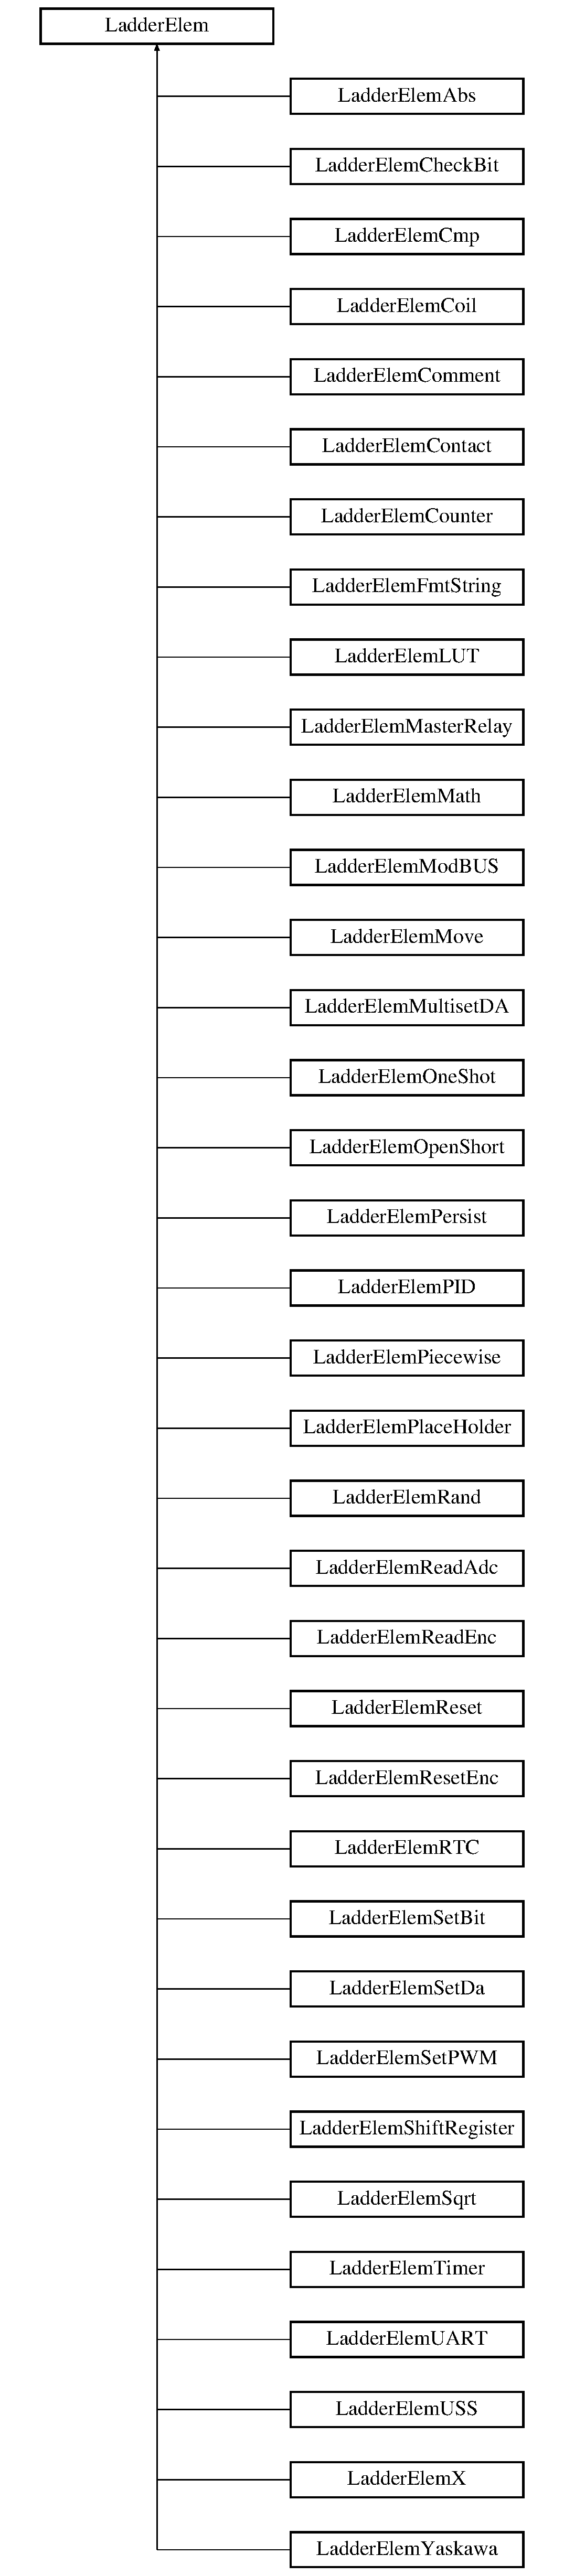
\includegraphics[height=12.000000cm]{class_ladder_elem}
\end{center}
\end{figure}
\subsection*{Classes}
\begin{DoxyCompactItemize}
\item 
union \hyperlink{union_ladder_elem_1_1_undo_redo_data}{Undo\-Redo\-Data}
\end{DoxyCompactItemize}
\subsection*{Public Member Functions}
\begin{DoxyCompactItemize}
\item 
\hypertarget{class_ladder_elem_a502ddd7d70be71002b99313d7e1dcdd5}{{\bfseries Ladder\-Elem} (bool E\-O\-L, bool Comment, bool Formatted, bool U\-A\-R\-T, int elem\-Which)}\label{class_ladder_elem_a502ddd7d70be71002b99313d7e1dcdd5}

\item 
\hypertarget{class_ladder_elem_a781692db86abe1d586e8837945b2ed38}{virtual pair$<$ string, string $>$ {\bfseries Draw\-T\-X\-T} (void)=0}\label{class_ladder_elem_a781692db86abe1d586e8837945b2ed38}

\item 
\hypertarget{class_ladder_elem_ac6a95244d693eb119fe26a46bfffc29f}{virtual bool {\bfseries Draw\-G\-U\-I} (bool powered\-Before, void $\ast$data)=0}\label{class_ladder_elem_ac6a95244d693eb119fe26a46bfffc29f}

\item 
\hypertarget{class_ladder_elem_a81500d77c2a73411bf4ffb317d385005}{virtual bool {\bfseries Show\-Dialog} (\hyperlink{struct_ladder_context}{Ladder\-Context} context)=0}\label{class_ladder_elem_a81500d77c2a73411bf4ffb317d385005}

\item 
\hypertarget{class_ladder_elem_a0de8dcca285f79a92d1d986b73b91a8a}{bool {\bfseries Generate\-Int\-Code} (\hyperlink{class_int_code}{Int\-Code} \&ic)}\label{class_ladder_elem_a0de8dcca285f79a92d1d986b73b91a8a}

\item 
\hypertarget{class_ladder_elem_a181e249958bc9db083d332f9c0a743bf}{bool {\bfseries Is\-Comment} (void)}\label{class_ladder_elem_a181e249958bc9db083d332f9c0a743bf}

\item 
\hypertarget{class_ladder_elem_a85fc6642a02d3e1d21e38b137d0e28b9}{bool {\bfseries Is\-E\-O\-L} (void)}\label{class_ladder_elem_a85fc6642a02d3e1d21e38b137d0e28b9}

\item 
\hypertarget{class_ladder_elem_a684c0eb890c674a55783bc94315c5775}{bool {\bfseries Is\-Powered\-After} (void)}\label{class_ladder_elem_a684c0eb890c674a55783bc94315c5775}

\item 
\hypertarget{class_ladder_elem_a574a88ffbd2b9d09947d3d117347ece8}{bool {\bfseries Is\-Formatted} (void)}\label{class_ladder_elem_a574a88ffbd2b9d09947d3d117347ece8}

\item 
\hypertarget{class_ladder_elem_aa582b254dac1c5846ed3a36e8de467ef}{bool {\bfseries Is\-U\-A\-R\-T} (void)}\label{class_ladder_elem_aa582b254dac1c5846ed3a36e8de467ef}

\item 
\hypertarget{class_ladder_elem_a110042ee8c22a1de7c882ad24ac0ef3c}{int {\bfseries get\-Which} (void)}\label{class_ladder_elem_a110042ee8c22a1de7c882ad24ac0ef3c}

\item 
\hypertarget{class_ladder_elem_abcac57389e52a25a1701f36a8d8734bf}{\hyperlink{class_ladder_diagram}{Ladder\-Diagram} $\ast$ {\bfseries get\-Diagram} (void)}\label{class_ladder_elem_abcac57389e52a25a1701f36a8d8734bf}

\item 
\hypertarget{class_ladder_elem_a55c140c849baadb2405afec5edf99412}{void {\bfseries set\-Diagram} (\hyperlink{class_ladder_diagram}{Ladder\-Diagram} $\ast$new\-Diagram)}\label{class_ladder_elem_a55c140c849baadb2405afec5edf99412}

\item 
\hypertarget{class_ladder_elem_a5ed7127003bc4bff193de746d6a3e85c}{virtual bool {\bfseries Can\-Insert} (\hyperlink{struct_ladder_context}{Ladder\-Context} context)=0}\label{class_ladder_elem_a5ed7127003bc4bff193de746d6a3e85c}

\item 
\hypertarget{class_ladder_elem_a2a670f63e40604bc86f55ff708a05603}{virtual void {\bfseries do\-Post\-Insert} (void)=0}\label{class_ladder_elem_a2a670f63e40604bc86f55ff708a05603}

\item 
\hypertarget{class_ladder_elem_a1b30da331f1638d23e3860f08d7dac69}{virtual void {\bfseries do\-Post\-Remove} (void)=0}\label{class_ladder_elem_a1b30da331f1638d23e3860f08d7dac69}

\item 
\hypertarget{class_ladder_elem_a947f2c620ff0e47d42c4e07ae1a60f64}{virtual int {\bfseries get\-Width\-T\-X\-T} (void)=0}\label{class_ladder_elem_a947f2c620ff0e47d42c4e07ae1a60f64}

\item 
\hypertarget{class_ladder_elem_a7ac5007e4cdf921b401f287fe0a967ab}{void {\bfseries set\-Properties} (\hyperlink{struct_ladder_context}{Ladder\-Context} context, void $\ast$prop\-Data)}\label{class_ladder_elem_a7ac5007e4cdf921b401f287fe0a967ab}

\item 
\hypertarget{class_ladder_elem_aa849dd21010eb6f6e46e18ef6560c556}{virtual void $\ast$ {\bfseries get\-Properties} (void)=0}\label{class_ladder_elem_aa849dd21010eb6f6e46e18ef6560c556}

\item 
\hypertarget{class_ladder_elem_a303166a93d0cae8a9b3a6b418cd4b3f0}{virtual \hyperlink{class_ladder_elem}{Ladder\-Elem} $\ast$ {\bfseries Clone} (\hyperlink{class_ladder_diagram}{Ladder\-Diagram} $\ast$diagram)=0}\label{class_ladder_elem_a303166a93d0cae8a9b3a6b418cd4b3f0}

\item 
\hypertarget{class_ladder_elem_ad2a5f2906ca4545d61c59aaa5bbb8532}{virtual bool {\bfseries accept\-I\-O} (unsigned long id, e\-Type type)=0}\label{class_ladder_elem_ad2a5f2906ca4545d61c59aaa5bbb8532}

\item 
\hypertarget{class_ladder_elem_af4cd0b1d17797fff4ac6d3c6ffa7f1fa}{virtual void {\bfseries update\-I\-O} (\hyperlink{class_ladder_diagram}{Ladder\-Diagram} $\ast$owner, bool is\-Discard)=0}\label{class_ladder_elem_af4cd0b1d17797fff4ac6d3c6ffa7f1fa}

\item 
\hypertarget{class_ladder_elem_a582660df6d2ca86b3da1850bd1b0b0b8}{virtual e\-Type {\bfseries get\-Allowed\-Type\-I\-O} (unsigned long id)=0}\label{class_ladder_elem_a582660df6d2ca86b3da1850bd1b0b0b8}

\item 
\hypertarget{class_ladder_elem_a87d5a1f182ec0907ce83f43bbb1fa836}{virtual int {\bfseries Search\-And\-Replace} (unsigned long id\-Search, string s\-New\-Text, bool is\-Replace)=0}\label{class_ladder_elem_a87d5a1f182ec0907ce83f43bbb1fa836}

\item 
\hypertarget{class_ladder_elem_aacbd85d07d925941a6c142ca06c42c8c}{bool {\bfseries update\-Name\-Type\-I\-O} (unsigned int index, string name, e\-Type type)}\label{class_ladder_elem_aacbd85d07d925941a6c142ca06c42c8c}

\item 
\hypertarget{class_ladder_elem_a23ddcab7515c6686f8e6cd3f7698030e}{bool {\bfseries Save} (F\-I\-L\-E $\ast$f)}\label{class_ladder_elem_a23ddcab7515c6686f8e6cd3f7698030e}

\item 
\hypertarget{class_ladder_elem_ae4be9df611a11ca978661b00af35117b}{bool {\bfseries Load} (F\-I\-L\-E $\ast$f, unsigned int version)}\label{class_ladder_elem_ae4be9df611a11ca978661b00af35117b}

\item 
\hypertarget{class_ladder_elem_a0c71aa34ef6e51563b06900853e0e8ac}{bool {\bfseries Do\-Undo\-Redo} (bool Is\-Undo, bool is\-Discard, \hyperlink{struct_undo_redo_action}{Undo\-Redo\-Action} \&action)}\label{class_ladder_elem_a0c71aa34ef6e51563b06900853e0e8ac}

\end{DoxyCompactItemize}
\subsection*{Protected Types}
\begin{DoxyCompactItemize}
\item 
enum {\bfseries Undo\-Redo\-Actions\-Enum} \{ {\bfseries e\-Checkpoint} = 0, 
{\bfseries e\-Set\-Prop}, 
{\bfseries e\-Actions\-End}
 \}
\end{DoxyCompactItemize}
\subsection*{Protected Attributes}
\begin{DoxyCompactItemize}
\item 
\hypertarget{class_ladder_elem_a8ad6b449a2fe3b72e5ed4339ee18a1a4}{bool {\bfseries powered\-After}}\label{class_ladder_elem_a8ad6b449a2fe3b72e5ed4339ee18a1a4}

\item 
\hypertarget{class_ladder_elem_a12087129f76e7020d1f85750766c9647}{\hyperlink{class_ladder_diagram}{Ladder\-Diagram} $\ast$ {\bfseries Diagram}}\label{class_ladder_elem_a12087129f76e7020d1f85750766c9647}

\end{DoxyCompactItemize}


The documentation for this class was generated from the following files\-:\begin{DoxyCompactItemize}
\item 
F\-:/\-S\-V\-N/\-P\-O\-P\-Tools/Ladder\-Objects.\-h\item 
F\-:/\-S\-V\-N/\-P\-O\-P\-Tools/Ladder\-Objects.\-cpp\end{DoxyCompactItemize}

\hypertarget{class_ladder_elem_abs}{\section{Ladder\-Elem\-Abs Class Reference}
\label{class_ladder_elem_abs}\index{Ladder\-Elem\-Abs@{Ladder\-Elem\-Abs}}
}
Inheritance diagram for Ladder\-Elem\-Abs\-:\begin{figure}[H]
\begin{center}
\leavevmode
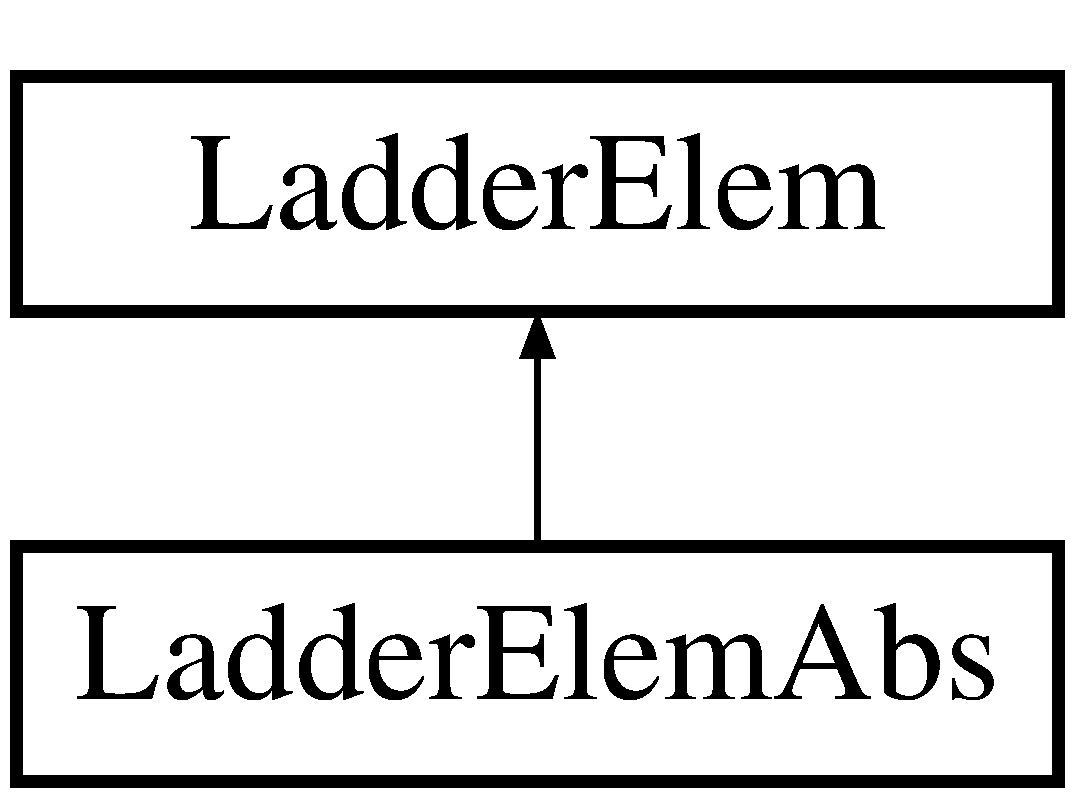
\includegraphics[height=2.000000cm]{class_ladder_elem_abs}
\end{center}
\end{figure}
\subsection*{Public Member Functions}
\begin{DoxyCompactItemize}
\item 
\hypertarget{class_ladder_elem_abs_a077f3a98f4ec4e57ca2f4773c4088daa}{{\bfseries Ladder\-Elem\-Abs} (\hyperlink{class_ladder_diagram}{Ladder\-Diagram} $\ast$diagram)}\label{class_ladder_elem_abs_a077f3a98f4ec4e57ca2f4773c4088daa}

\item 
\hypertarget{class_ladder_elem_abs_ae8b2051ef419301e679973d32eae20c6}{pair$<$ string, string $>$ {\bfseries Draw\-T\-X\-T} (void)}\label{class_ladder_elem_abs_ae8b2051ef419301e679973d32eae20c6}

\item 
\hypertarget{class_ladder_elem_abs_af5fa3f84f9ef991409d4fea9a6dc6137}{bool {\bfseries Draw\-G\-U\-I} (bool powered\-Before, void $\ast$data)}\label{class_ladder_elem_abs_af5fa3f84f9ef991409d4fea9a6dc6137}

\item 
\hypertarget{class_ladder_elem_abs_a43292e9cd8eb63f935afe7d46636629f}{bool {\bfseries Show\-Dialog} (\hyperlink{struct_ladder_context}{Ladder\-Context} context)}\label{class_ladder_elem_abs_a43292e9cd8eb63f935afe7d46636629f}

\item 
\hypertarget{class_ladder_elem_abs_a5453dad1e55023e12a9d5ffaa29449b3}{bool {\bfseries internal\-Generate\-Int\-Code} (\hyperlink{class_int_code}{Int\-Code} \&ic)}\label{class_ladder_elem_abs_a5453dad1e55023e12a9d5ffaa29449b3}

\item 
\hypertarget{class_ladder_elem_abs_aaa0e932f6fb7cd347cb0c1a520b5cc98}{void $\ast$ {\bfseries get\-Properties} (void)}\label{class_ladder_elem_abs_aaa0e932f6fb7cd347cb0c1a520b5cc98}

\item 
\hypertarget{class_ladder_elem_abs_a27bbfad73138bc8273ce15b073d69eba}{bool {\bfseries Can\-Insert} (\hyperlink{struct_ladder_context}{Ladder\-Context} context)}\label{class_ladder_elem_abs_a27bbfad73138bc8273ce15b073d69eba}

\item 
\hypertarget{class_ladder_elem_abs_a38d099f307f87782e137f23d201e69bc}{void {\bfseries do\-Post\-Insert} (void)}\label{class_ladder_elem_abs_a38d099f307f87782e137f23d201e69bc}

\item 
\hypertarget{class_ladder_elem_abs_aa0c3b78bc6066034bd8a074aa3b47e02}{void {\bfseries do\-Post\-Remove} (void)}\label{class_ladder_elem_abs_aa0c3b78bc6066034bd8a074aa3b47e02}

\item 
\hypertarget{class_ladder_elem_abs_aba7f630f18f97f58a51863b3cc061df3}{int {\bfseries get\-Width\-T\-X\-T} (void)}\label{class_ladder_elem_abs_aba7f630f18f97f58a51863b3cc061df3}

\item 
\hypertarget{class_ladder_elem_abs_a4cc6f65b22cdfe868bc3504984a6d09c}{\hyperlink{class_ladder_elem}{Ladder\-Elem} $\ast$ {\bfseries Clone} (\hyperlink{class_ladder_diagram}{Ladder\-Diagram} $\ast$diagram)}\label{class_ladder_elem_abs_a4cc6f65b22cdfe868bc3504984a6d09c}

\item 
\hypertarget{class_ladder_elem_abs_a7bc936e05441d687da2363cde9fbcd1a}{bool {\bfseries accept\-I\-O} (unsigned long id, e\-Type type)}\label{class_ladder_elem_abs_a7bc936e05441d687da2363cde9fbcd1a}

\item 
\hypertarget{class_ladder_elem_abs_a47775f0ec46039939b42e4ee1c18ecd8}{void {\bfseries update\-I\-O} (\hyperlink{class_ladder_diagram}{Ladder\-Diagram} $\ast$owner, bool is\-Discard)}\label{class_ladder_elem_abs_a47775f0ec46039939b42e4ee1c18ecd8}

\item 
\hypertarget{class_ladder_elem_abs_a63c91a6c18a0f6a6df69196bd613e596}{e\-Type {\bfseries get\-Allowed\-Type\-I\-O} (unsigned long id)}\label{class_ladder_elem_abs_a63c91a6c18a0f6a6df69196bd613e596}

\item 
\hypertarget{class_ladder_elem_abs_a8dfac6da42c1593feed12ae6dd8204da}{int {\bfseries Search\-And\-Replace} (unsigned long id\-Search, string s\-New\-Text, bool is\-Replace)}\label{class_ladder_elem_abs_a8dfac6da42c1593feed12ae6dd8204da}

\item 
\hypertarget{class_ladder_elem_abs_a80edab4fbf174ea96d3a8038c86a7adc}{bool {\bfseries internal\-Do\-Undo\-Redo} (bool Is\-Undo, bool is\-Discard, \hyperlink{struct_undo_redo_action}{Undo\-Redo\-Action} \&action)}\label{class_ladder_elem_abs_a80edab4fbf174ea96d3a8038c86a7adc}

\end{DoxyCompactItemize}
\subsection*{Additional Inherited Members}


The documentation for this class was generated from the following files\-:\begin{DoxyCompactItemize}
\item 
F\-:/\-S\-V\-N/\-P\-O\-P\-Tools/Ladder\-Objects.\-h\item 
F\-:/\-S\-V\-N/\-P\-O\-P\-Tools/Ladder\-G\-U\-I.\-cpp\item 
F\-:/\-S\-V\-N/\-P\-O\-P\-Tools/Ladder\-Objects.\-cpp\end{DoxyCompactItemize}

\hypertarget{struct_ladder_elem_abs_prop}{\section{Ladder\-Elem\-Abs\-Prop Struct Reference}
\label{struct_ladder_elem_abs_prop}\index{Ladder\-Elem\-Abs\-Prop@{Ladder\-Elem\-Abs\-Prop}}
}
\subsection*{Public Attributes}
\begin{DoxyCompactItemize}
\item 
\hypertarget{struct_ladder_elem_abs_prop_a38ba59d87c659e1ce0a1dc7b67fbe8a2}{pair$<$ unsigned long, int $>$ {\bfseries id\-Dest}}\label{struct_ladder_elem_abs_prop_a38ba59d87c659e1ce0a1dc7b67fbe8a2}

\item 
\hypertarget{struct_ladder_elem_abs_prop_a1df5c251b61ae7cd420a34b02a5dbf12}{pair$<$ unsigned long, int $>$ {\bfseries id\-Src}}\label{struct_ladder_elem_abs_prop_a1df5c251b61ae7cd420a34b02a5dbf12}

\end{DoxyCompactItemize}


The documentation for this struct was generated from the following file\-:\begin{DoxyCompactItemize}
\item 
F\-:/\-S\-V\-N/\-P\-O\-P\-Tools/Ladder\-Objects.\-h\end{DoxyCompactItemize}

\hypertarget{class_ladder_elem_check_bit}{\section{Ladder\-Elem\-Check\-Bit Class Reference}
\label{class_ladder_elem_check_bit}\index{Ladder\-Elem\-Check\-Bit@{Ladder\-Elem\-Check\-Bit}}
}
Inheritance diagram for Ladder\-Elem\-Check\-Bit\-:\begin{figure}[H]
\begin{center}
\leavevmode
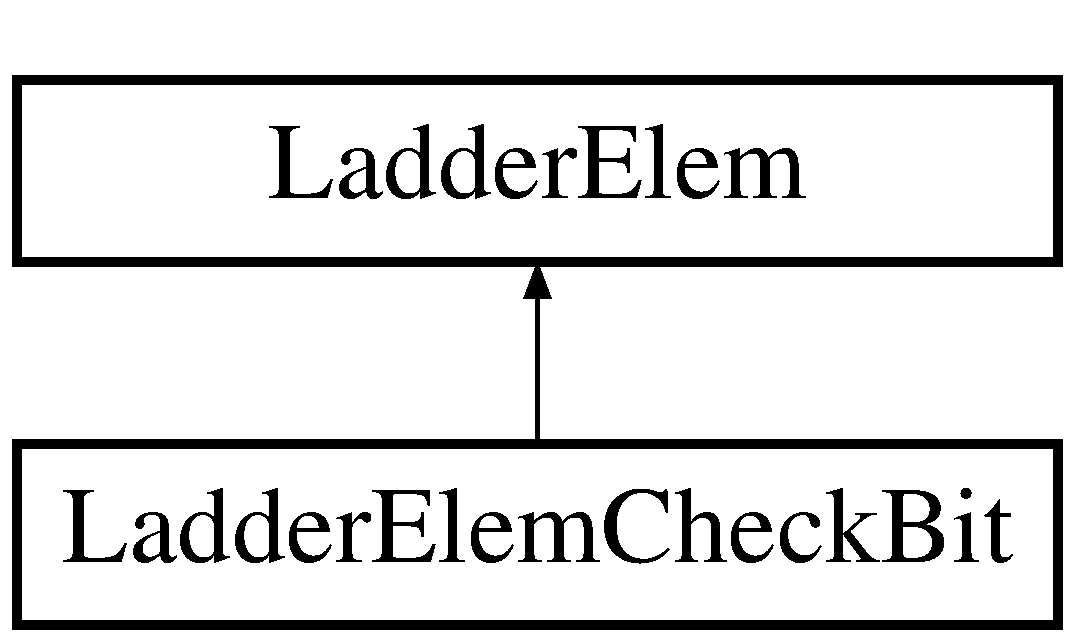
\includegraphics[height=2.000000cm]{class_ladder_elem_check_bit}
\end{center}
\end{figure}
\subsection*{Public Member Functions}
\begin{DoxyCompactItemize}
\item 
\hypertarget{class_ladder_elem_check_bit_a300f920d34550a52a473a906d553f2c9}{{\bfseries Ladder\-Elem\-Check\-Bit} (\hyperlink{class_ladder_diagram}{Ladder\-Diagram} $\ast$diagram)}\label{class_ladder_elem_check_bit_a300f920d34550a52a473a906d553f2c9}

\item 
\hypertarget{class_ladder_elem_check_bit_a89005c6f18b5f88858de1db0a64b1ab1}{pair$<$ string, string $>$ {\bfseries Draw\-T\-X\-T} (void)}\label{class_ladder_elem_check_bit_a89005c6f18b5f88858de1db0a64b1ab1}

\item 
\hypertarget{class_ladder_elem_check_bit_ab50ef084b81c2b227b1fc5a97d0b38a1}{bool {\bfseries Draw\-G\-U\-I} (bool powered\-Before, void $\ast$data)}\label{class_ladder_elem_check_bit_ab50ef084b81c2b227b1fc5a97d0b38a1}

\item 
\hypertarget{class_ladder_elem_check_bit_a592260a058269a68da595ee161b94593}{bool {\bfseries Show\-Dialog} (\hyperlink{struct_ladder_context}{Ladder\-Context} context)}\label{class_ladder_elem_check_bit_a592260a058269a68da595ee161b94593}

\item 
\hypertarget{class_ladder_elem_check_bit_aba768cd7355c3754219fff439265fd74}{bool {\bfseries internal\-Generate\-Int\-Code} (\hyperlink{class_int_code}{Int\-Code} \&ic)}\label{class_ladder_elem_check_bit_aba768cd7355c3754219fff439265fd74}

\item 
\hypertarget{class_ladder_elem_check_bit_af4b78435d266642950759ca4cea843b8}{void $\ast$ {\bfseries get\-Properties} (void)}\label{class_ladder_elem_check_bit_af4b78435d266642950759ca4cea843b8}

\item 
\hypertarget{class_ladder_elem_check_bit_a4ffeb46e98d7deaf8882905898c288de}{bool {\bfseries Can\-Insert} (\hyperlink{struct_ladder_context}{Ladder\-Context} context)}\label{class_ladder_elem_check_bit_a4ffeb46e98d7deaf8882905898c288de}

\item 
\hypertarget{class_ladder_elem_check_bit_a45fb3a81046f13aa400b7674ecece7ca}{void {\bfseries do\-Post\-Insert} (void)}\label{class_ladder_elem_check_bit_a45fb3a81046f13aa400b7674ecece7ca}

\item 
\hypertarget{class_ladder_elem_check_bit_a32dc1a1f04bca1f0f21e7eb06b123c73}{void {\bfseries do\-Post\-Remove} (void)}\label{class_ladder_elem_check_bit_a32dc1a1f04bca1f0f21e7eb06b123c73}

\item 
\hypertarget{class_ladder_elem_check_bit_aea01b38859c4546387462945864a5840}{int {\bfseries get\-Width\-T\-X\-T} (void)}\label{class_ladder_elem_check_bit_aea01b38859c4546387462945864a5840}

\item 
\hypertarget{class_ladder_elem_check_bit_aadda7dc5eb5649ae7670029760be8369}{\hyperlink{class_ladder_elem}{Ladder\-Elem} $\ast$ {\bfseries Clone} (\hyperlink{class_ladder_diagram}{Ladder\-Diagram} $\ast$diagram)}\label{class_ladder_elem_check_bit_aadda7dc5eb5649ae7670029760be8369}

\item 
\hypertarget{class_ladder_elem_check_bit_abc126ebd82f3885e1ccdd60f5dc25158}{bool {\bfseries accept\-I\-O} (unsigned long id, e\-Type type)}\label{class_ladder_elem_check_bit_abc126ebd82f3885e1ccdd60f5dc25158}

\item 
\hypertarget{class_ladder_elem_check_bit_ac90b97a2ae061fdff1f242f4bcfac8fe}{void {\bfseries update\-I\-O} (\hyperlink{class_ladder_diagram}{Ladder\-Diagram} $\ast$owner, bool is\-Discard)}\label{class_ladder_elem_check_bit_ac90b97a2ae061fdff1f242f4bcfac8fe}

\item 
\hypertarget{class_ladder_elem_check_bit_a3e1560a879b183de83a0065848c49acc}{e\-Type {\bfseries get\-Allowed\-Type\-I\-O} (unsigned long id)}\label{class_ladder_elem_check_bit_a3e1560a879b183de83a0065848c49acc}

\item 
\hypertarget{class_ladder_elem_check_bit_a0eac533b5f07d7a546162d0398295fb0}{int {\bfseries Search\-And\-Replace} (unsigned long id\-Search, string s\-New\-Text, bool is\-Replace)}\label{class_ladder_elem_check_bit_a0eac533b5f07d7a546162d0398295fb0}

\item 
\hypertarget{class_ladder_elem_check_bit_a427fd990acbbae6ac81e291cd4aeed93}{bool {\bfseries internal\-Do\-Undo\-Redo} (bool Is\-Undo, bool is\-Discard, \hyperlink{struct_undo_redo_action}{Undo\-Redo\-Action} \&action)}\label{class_ladder_elem_check_bit_a427fd990acbbae6ac81e291cd4aeed93}

\end{DoxyCompactItemize}
\subsection*{Additional Inherited Members}


The documentation for this class was generated from the following files\-:\begin{DoxyCompactItemize}
\item 
F\-:/\-S\-V\-N/\-P\-O\-P\-Tools/Ladder\-Objects.\-h\item 
F\-:/\-S\-V\-N/\-P\-O\-P\-Tools/Ladder\-G\-U\-I.\-cpp\item 
F\-:/\-S\-V\-N/\-P\-O\-P\-Tools/Ladder\-Objects.\-cpp\end{DoxyCompactItemize}

\hypertarget{struct_ladder_elem_check_bit_prop}{\section{Ladder\-Elem\-Check\-Bit\-Prop Struct Reference}
\label{struct_ladder_elem_check_bit_prop}\index{Ladder\-Elem\-Check\-Bit\-Prop@{Ladder\-Elem\-Check\-Bit\-Prop}}
}
\subsection*{Public Attributes}
\begin{DoxyCompactItemize}
\item 
\hypertarget{struct_ladder_elem_check_bit_prop_a894f61904e2736ab103be84f44e12a9e}{pair$<$ unsigned long, int $>$ {\bfseries id\-Name}}\label{struct_ladder_elem_check_bit_prop_a894f61904e2736ab103be84f44e12a9e}

\item 
\hypertarget{struct_ladder_elem_check_bit_prop_aa2bf712bfe21b69416f09aa870b64e0b}{int {\bfseries bit}}\label{struct_ladder_elem_check_bit_prop_aa2bf712bfe21b69416f09aa870b64e0b}

\item 
\hypertarget{struct_ladder_elem_check_bit_prop_a89cc8a744143f278422dd7380295e3d4}{bool {\bfseries set}}\label{struct_ladder_elem_check_bit_prop_a89cc8a744143f278422dd7380295e3d4}

\end{DoxyCompactItemize}


The documentation for this struct was generated from the following file\-:\begin{DoxyCompactItemize}
\item 
F\-:/\-S\-V\-N/\-P\-O\-P\-Tools/Ladder\-Objects.\-h\end{DoxyCompactItemize}

\hypertarget{class_ladder_elem_cmp}{\section{Ladder\-Elem\-Cmp Class Reference}
\label{class_ladder_elem_cmp}\index{Ladder\-Elem\-Cmp@{Ladder\-Elem\-Cmp}}
}
Inheritance diagram for Ladder\-Elem\-Cmp\-:\begin{figure}[H]
\begin{center}
\leavevmode
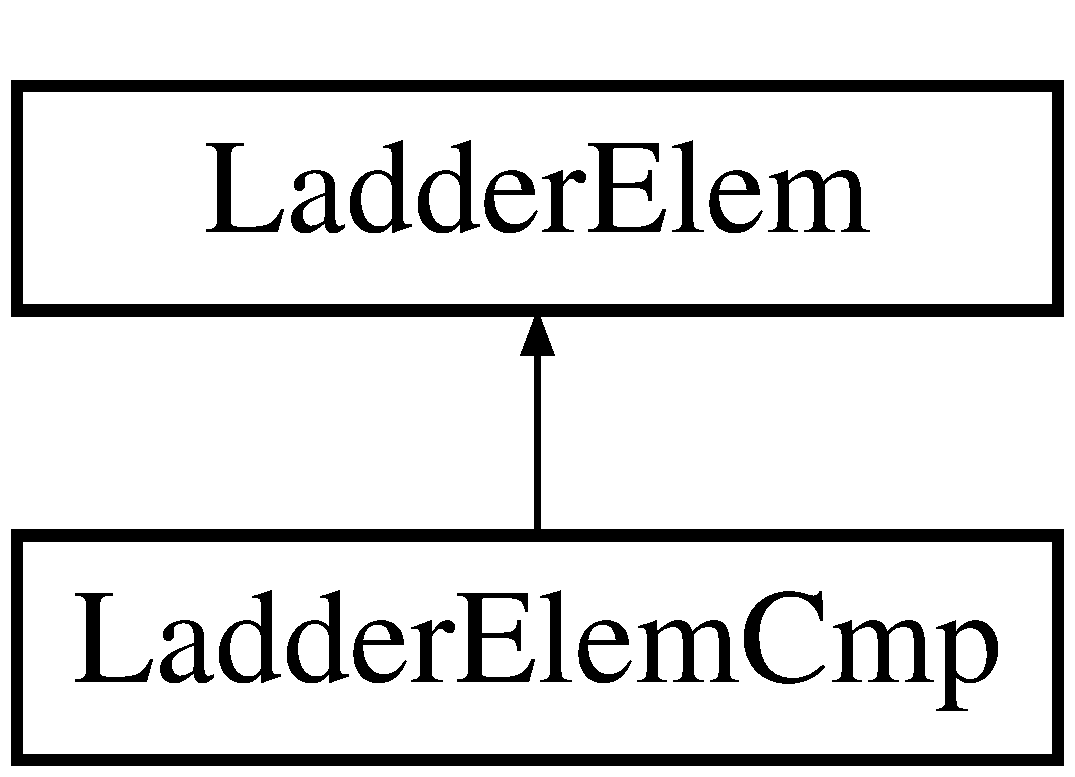
\includegraphics[height=2.000000cm]{class_ladder_elem_cmp}
\end{center}
\end{figure}
\subsection*{Public Member Functions}
\begin{DoxyCompactItemize}
\item 
\hypertarget{class_ladder_elem_cmp_a7773a5bfe30b476a23d6cd667a7dcc66}{{\bfseries Ladder\-Elem\-Cmp} (\hyperlink{class_ladder_diagram}{Ladder\-Diagram} $\ast$diagram, int which)}\label{class_ladder_elem_cmp_a7773a5bfe30b476a23d6cd667a7dcc66}

\item 
\hypertarget{class_ladder_elem_cmp_a6b7bdfddbb2d5f3f2775a50bd1659652}{pair$<$ string, string $>$ {\bfseries Draw\-T\-X\-T} (void)}\label{class_ladder_elem_cmp_a6b7bdfddbb2d5f3f2775a50bd1659652}

\item 
\hypertarget{class_ladder_elem_cmp_a75e4aa7bc34311cb04956525713a2d96}{bool {\bfseries Draw\-G\-U\-I} (bool powered\-Before, void $\ast$data)}\label{class_ladder_elem_cmp_a75e4aa7bc34311cb04956525713a2d96}

\item 
\hypertarget{class_ladder_elem_cmp_a16f28f71fdba2a692680d7b7a3f48a3b}{bool {\bfseries Show\-Dialog} (\hyperlink{struct_ladder_context}{Ladder\-Context} context)}\label{class_ladder_elem_cmp_a16f28f71fdba2a692680d7b7a3f48a3b}

\item 
\hypertarget{class_ladder_elem_cmp_a9bb37cfff313aed38ad82be94bc533ac}{bool {\bfseries internal\-Generate\-Int\-Code} (\hyperlink{class_int_code}{Int\-Code} \&ic)}\label{class_ladder_elem_cmp_a9bb37cfff313aed38ad82be94bc533ac}

\item 
\hypertarget{class_ladder_elem_cmp_a40247762fb1e1efd0b299eaafe40d80f}{void $\ast$ {\bfseries get\-Properties} (void)}\label{class_ladder_elem_cmp_a40247762fb1e1efd0b299eaafe40d80f}

\item 
\hypertarget{class_ladder_elem_cmp_a9b9a27b425875dbd197e1412f381fd5d}{bool {\bfseries Can\-Insert} (\hyperlink{struct_ladder_context}{Ladder\-Context} context)}\label{class_ladder_elem_cmp_a9b9a27b425875dbd197e1412f381fd5d}

\item 
\hypertarget{class_ladder_elem_cmp_acd4a0c266bf429bd9b96a4ce88ad93c2}{void {\bfseries do\-Post\-Insert} (void)}\label{class_ladder_elem_cmp_acd4a0c266bf429bd9b96a4ce88ad93c2}

\item 
\hypertarget{class_ladder_elem_cmp_a46f387413a1e82da59fe74712452af94}{void {\bfseries do\-Post\-Remove} (void)}\label{class_ladder_elem_cmp_a46f387413a1e82da59fe74712452af94}

\item 
\hypertarget{class_ladder_elem_cmp_aa95abbcf6d26c88e39cd56c056515785}{int {\bfseries get\-Width\-T\-X\-T} (void)}\label{class_ladder_elem_cmp_aa95abbcf6d26c88e39cd56c056515785}

\item 
\hypertarget{class_ladder_elem_cmp_add3faa0d8dcff6824115b2506438a684}{\hyperlink{class_ladder_elem}{Ladder\-Elem} $\ast$ {\bfseries Clone} (\hyperlink{class_ladder_diagram}{Ladder\-Diagram} $\ast$diagram)}\label{class_ladder_elem_cmp_add3faa0d8dcff6824115b2506438a684}

\item 
\hypertarget{class_ladder_elem_cmp_a8765bb7842def3ebd22783b9fc6ffb92}{bool {\bfseries accept\-I\-O} (unsigned long id, e\-Type type)}\label{class_ladder_elem_cmp_a8765bb7842def3ebd22783b9fc6ffb92}

\item 
\hypertarget{class_ladder_elem_cmp_a3bbc0b5e97229b1b00e95ff7d4cf40c6}{void {\bfseries update\-I\-O} (\hyperlink{class_ladder_diagram}{Ladder\-Diagram} $\ast$owner, bool is\-Discard)}\label{class_ladder_elem_cmp_a3bbc0b5e97229b1b00e95ff7d4cf40c6}

\item 
\hypertarget{class_ladder_elem_cmp_a6143f94325bb1a0e8c867b32ee220e58}{e\-Type {\bfseries get\-Allowed\-Type\-I\-O} (unsigned long id)}\label{class_ladder_elem_cmp_a6143f94325bb1a0e8c867b32ee220e58}

\item 
\hypertarget{class_ladder_elem_cmp_a52e45ac06ec1d8b6002ae9f81a061fea}{int {\bfseries Search\-And\-Replace} (unsigned long id\-Search, string s\-New\-Text, bool is\-Replace)}\label{class_ladder_elem_cmp_a52e45ac06ec1d8b6002ae9f81a061fea}

\item 
\hypertarget{class_ladder_elem_cmp_a033729670c5afbb7d33f7fbfbe95dbe1}{bool {\bfseries internal\-Do\-Undo\-Redo} (bool Is\-Undo, bool is\-Discard, \hyperlink{struct_undo_redo_action}{Undo\-Redo\-Action} \&action)}\label{class_ladder_elem_cmp_a033729670c5afbb7d33f7fbfbe95dbe1}

\end{DoxyCompactItemize}
\subsection*{Additional Inherited Members}


The documentation for this class was generated from the following files\-:\begin{DoxyCompactItemize}
\item 
F\-:/\-S\-V\-N/\-P\-O\-P\-Tools/Ladder\-Objects.\-h\item 
F\-:/\-S\-V\-N/\-P\-O\-P\-Tools/Ladder\-G\-U\-I.\-cpp\item 
F\-:/\-S\-V\-N/\-P\-O\-P\-Tools/Ladder\-Objects.\-cpp\end{DoxyCompactItemize}

\hypertarget{struct_ladder_elem_cmp_prop}{\section{Ladder\-Elem\-Cmp\-Prop Struct Reference}
\label{struct_ladder_elem_cmp_prop}\index{Ladder\-Elem\-Cmp\-Prop@{Ladder\-Elem\-Cmp\-Prop}}
}
\subsection*{Public Attributes}
\begin{DoxyCompactItemize}
\item 
\hypertarget{struct_ladder_elem_cmp_prop_a1fa9d9b5ab714c275dd15b5f5a8167c6}{pair$<$ unsigned long, int $>$ {\bfseries id\-Op1}}\label{struct_ladder_elem_cmp_prop_a1fa9d9b5ab714c275dd15b5f5a8167c6}

\item 
\hypertarget{struct_ladder_elem_cmp_prop_a63a7929178421773f4451b3d75529473}{pair$<$ unsigned long, int $>$ {\bfseries id\-Op2}}\label{struct_ladder_elem_cmp_prop_a63a7929178421773f4451b3d75529473}

\end{DoxyCompactItemize}


The documentation for this struct was generated from the following file\-:\begin{DoxyCompactItemize}
\item 
F\-:/\-S\-V\-N/\-P\-O\-P\-Tools/Ladder\-Objects.\-h\end{DoxyCompactItemize}

\hypertarget{class_ladder_elem_coil}{\section{Ladder\-Elem\-Coil Class Reference}
\label{class_ladder_elem_coil}\index{Ladder\-Elem\-Coil@{Ladder\-Elem\-Coil}}
}
Inheritance diagram for Ladder\-Elem\-Coil\-:\begin{figure}[H]
\begin{center}
\leavevmode
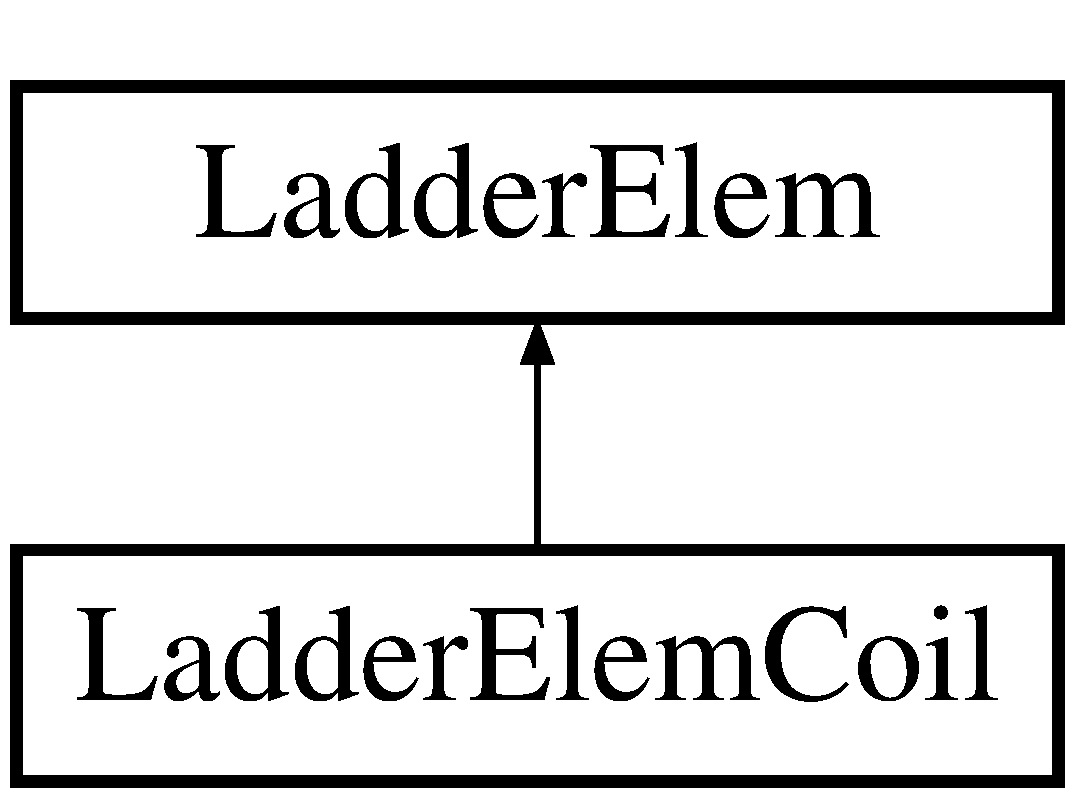
\includegraphics[height=2.000000cm]{class_ladder_elem_coil}
\end{center}
\end{figure}
\subsection*{Public Member Functions}
\begin{DoxyCompactItemize}
\item 
\hypertarget{class_ladder_elem_coil_afc4097323c943a8e43b21a7ae13f56fa}{{\bfseries Ladder\-Elem\-Coil} (\hyperlink{class_ladder_diagram}{Ladder\-Diagram} $\ast$diagram)}\label{class_ladder_elem_coil_afc4097323c943a8e43b21a7ae13f56fa}

\item 
\hypertarget{class_ladder_elem_coil_a7025841d963fea006eba83659a37a060}{pair$<$ string, string $>$ {\bfseries Draw\-T\-X\-T} (void)}\label{class_ladder_elem_coil_a7025841d963fea006eba83659a37a060}

\item 
\hypertarget{class_ladder_elem_coil_a6f8610f700c71ecff39c290005009d22}{bool {\bfseries Draw\-G\-U\-I} (bool powered\-Before, void $\ast$data)}\label{class_ladder_elem_coil_a6f8610f700c71ecff39c290005009d22}

\item 
\hypertarget{class_ladder_elem_coil_a70efa09fe043c1cb1f79623ea86d0e4f}{bool {\bfseries Show\-Dialog} (\hyperlink{struct_ladder_context}{Ladder\-Context} context)}\label{class_ladder_elem_coil_a70efa09fe043c1cb1f79623ea86d0e4f}

\item 
\hypertarget{class_ladder_elem_coil_a8b4ddc5a8a7c98049231f5bd73437ec9}{bool {\bfseries internal\-Generate\-Int\-Code} (\hyperlink{class_int_code}{Int\-Code} \&ic)}\label{class_ladder_elem_coil_a8b4ddc5a8a7c98049231f5bd73437ec9}

\item 
\hypertarget{class_ladder_elem_coil_a1cc313d369e046e6dcdfd464e634857f}{void $\ast$ {\bfseries get\-Properties} (void)}\label{class_ladder_elem_coil_a1cc313d369e046e6dcdfd464e634857f}

\item 
\hypertarget{class_ladder_elem_coil_ae8496d24dde35c746d7a162030f51a21}{bool {\bfseries Can\-Insert} (\hyperlink{struct_ladder_context}{Ladder\-Context} context)}\label{class_ladder_elem_coil_ae8496d24dde35c746d7a162030f51a21}

\item 
\hypertarget{class_ladder_elem_coil_aa694376d58d01dd6bae606bbda13b8d7}{void {\bfseries do\-Post\-Insert} (void)}\label{class_ladder_elem_coil_aa694376d58d01dd6bae606bbda13b8d7}

\item 
\hypertarget{class_ladder_elem_coil_aa302b77085c225c60940ed6c1e22cc37}{void {\bfseries do\-Post\-Remove} (void)}\label{class_ladder_elem_coil_aa302b77085c225c60940ed6c1e22cc37}

\item 
\hypertarget{class_ladder_elem_coil_aac646ac0033f125edd7f3c759c955e51}{int {\bfseries get\-Width\-T\-X\-T} (void)}\label{class_ladder_elem_coil_aac646ac0033f125edd7f3c759c955e51}

\item 
\hypertarget{class_ladder_elem_coil_a74911fc095b6b53a09ccd4acc4bd5278}{\hyperlink{class_ladder_elem}{Ladder\-Elem} $\ast$ {\bfseries Clone} (\hyperlink{class_ladder_diagram}{Ladder\-Diagram} $\ast$diagram)}\label{class_ladder_elem_coil_a74911fc095b6b53a09ccd4acc4bd5278}

\item 
\hypertarget{class_ladder_elem_coil_aa035d6eb2d4d7d7f14f7cc59492f439a}{bool {\bfseries accept\-I\-O} (unsigned long id, e\-Type type)}\label{class_ladder_elem_coil_aa035d6eb2d4d7d7f14f7cc59492f439a}

\item 
\hypertarget{class_ladder_elem_coil_acc36e04d6f30c6d846f51d5e03bc3a72}{void {\bfseries update\-I\-O} (\hyperlink{class_ladder_diagram}{Ladder\-Diagram} $\ast$owner, bool is\-Discard)}\label{class_ladder_elem_coil_acc36e04d6f30c6d846f51d5e03bc3a72}

\item 
\hypertarget{class_ladder_elem_coil_a28bcaee25c7dc2c8fb1c6279097d58e6}{e\-Type {\bfseries get\-Allowed\-Type\-I\-O} (unsigned long id)}\label{class_ladder_elem_coil_a28bcaee25c7dc2c8fb1c6279097d58e6}

\item 
\hypertarget{class_ladder_elem_coil_a05396fa4991b584cbd5b9d174ad649f5}{int {\bfseries Search\-And\-Replace} (unsigned long id\-Search, string s\-New\-Text, bool is\-Replace)}\label{class_ladder_elem_coil_a05396fa4991b584cbd5b9d174ad649f5}

\item 
\hypertarget{class_ladder_elem_coil_a8e8a4ed83d3627fc91d2bed6bb86fc3d}{bool {\bfseries internal\-Do\-Undo\-Redo} (bool Is\-Undo, bool is\-Discard, \hyperlink{struct_undo_redo_action}{Undo\-Redo\-Action} \&action)}\label{class_ladder_elem_coil_a8e8a4ed83d3627fc91d2bed6bb86fc3d}

\end{DoxyCompactItemize}
\subsection*{Additional Inherited Members}


The documentation for this class was generated from the following files\-:\begin{DoxyCompactItemize}
\item 
F\-:/\-S\-V\-N/\-P\-O\-P\-Tools/Ladder\-Objects.\-h\item 
F\-:/\-S\-V\-N/\-P\-O\-P\-Tools/Ladder\-G\-U\-I.\-cpp\item 
F\-:/\-S\-V\-N/\-P\-O\-P\-Tools/Ladder\-Objects.\-cpp\end{DoxyCompactItemize}

\hypertarget{struct_ladder_elem_coil_prop}{\section{Ladder\-Elem\-Coil\-Prop Struct Reference}
\label{struct_ladder_elem_coil_prop}\index{Ladder\-Elem\-Coil\-Prop@{Ladder\-Elem\-Coil\-Prop}}
}
\subsection*{Public Attributes}
\begin{DoxyCompactItemize}
\item 
\hypertarget{struct_ladder_elem_coil_prop_ae2157e10379b4fbbcf88eb5073bde778}{bool {\bfseries negated}}\label{struct_ladder_elem_coil_prop_ae2157e10379b4fbbcf88eb5073bde778}

\item 
\hypertarget{struct_ladder_elem_coil_prop_af87ddbff2987d1837754c81efee17e08}{bool {\bfseries set\-Only}}\label{struct_ladder_elem_coil_prop_af87ddbff2987d1837754c81efee17e08}

\item 
\hypertarget{struct_ladder_elem_coil_prop_a94c89687fff6b1492cba65b7b88bd7fa}{bool {\bfseries reset\-Only}}\label{struct_ladder_elem_coil_prop_a94c89687fff6b1492cba65b7b88bd7fa}

\item 
\hypertarget{struct_ladder_elem_coil_prop_ae89d0b9b1918430836144316af84bf48}{pair$<$ unsigned long, int $>$ {\bfseries id\-Name}}\label{struct_ladder_elem_coil_prop_ae89d0b9b1918430836144316af84bf48}

\end{DoxyCompactItemize}


The documentation for this struct was generated from the following file\-:\begin{DoxyCompactItemize}
\item 
F\-:/\-S\-V\-N/\-P\-O\-P\-Tools/Ladder\-Objects.\-h\end{DoxyCompactItemize}

\hypertarget{class_ladder_elem_comment}{\section{Ladder\-Elem\-Comment Class Reference}
\label{class_ladder_elem_comment}\index{Ladder\-Elem\-Comment@{Ladder\-Elem\-Comment}}
}
Inheritance diagram for Ladder\-Elem\-Comment\-:\begin{figure}[H]
\begin{center}
\leavevmode
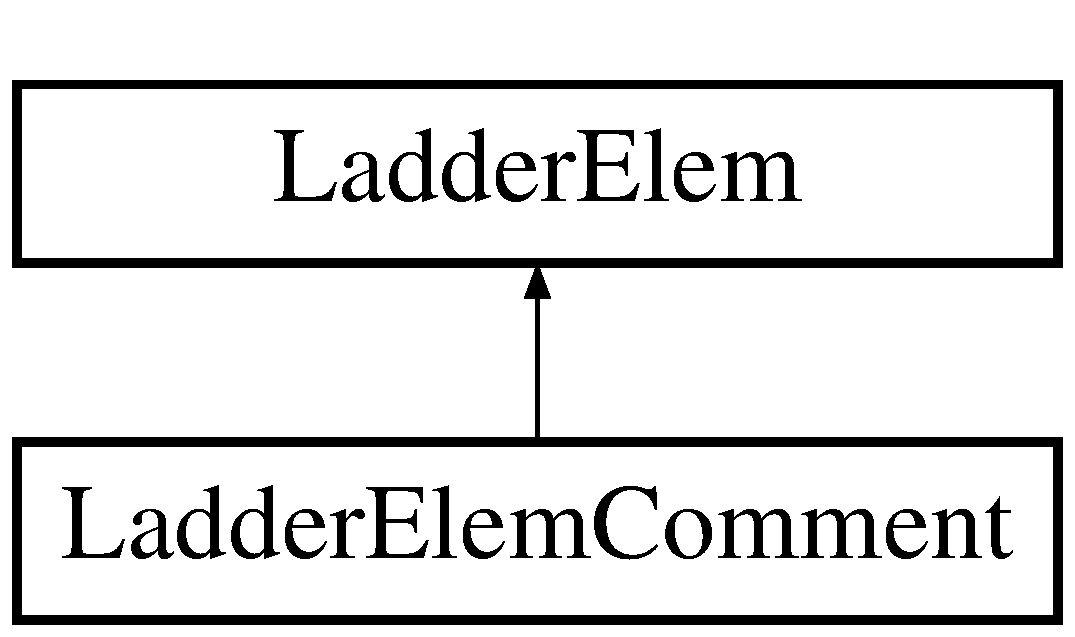
\includegraphics[height=2.000000cm]{class_ladder_elem_comment}
\end{center}
\end{figure}
\subsection*{Public Member Functions}
\begin{DoxyCompactItemize}
\item 
\hypertarget{class_ladder_elem_comment_a9656c1026e7b290febda5fe11154bec9}{{\bfseries Ladder\-Elem\-Comment} (\hyperlink{class_ladder_diagram}{Ladder\-Diagram} $\ast$diagram)}\label{class_ladder_elem_comment_a9656c1026e7b290febda5fe11154bec9}

\item 
\hypertarget{class_ladder_elem_comment_a7b38d0321b8aef5156866497fee5c463}{pair$<$ string, string $>$ {\bfseries Draw\-T\-X\-T} (void)}\label{class_ladder_elem_comment_a7b38d0321b8aef5156866497fee5c463}

\item 
\hypertarget{class_ladder_elem_comment_a62cf33a834d228f74272d20b4911221d}{bool {\bfseries Draw\-G\-U\-I} (bool powered\-Before, void $\ast$data)}\label{class_ladder_elem_comment_a62cf33a834d228f74272d20b4911221d}

\item 
\hypertarget{class_ladder_elem_comment_a8f9a3dbdc2264579adc0c4691a8051fd}{bool {\bfseries Show\-Dialog} (\hyperlink{struct_ladder_context}{Ladder\-Context} context)}\label{class_ladder_elem_comment_a8f9a3dbdc2264579adc0c4691a8051fd}

\item 
\hypertarget{class_ladder_elem_comment_a3b67d265b783b5ab76e82dbfab85baa3}{bool {\bfseries internal\-Generate\-Int\-Code} (\hyperlink{class_int_code}{Int\-Code} \&ic)}\label{class_ladder_elem_comment_a3b67d265b783b5ab76e82dbfab85baa3}

\item 
\hypertarget{class_ladder_elem_comment_a850ae79b96270352e6277c87736e7fba}{void $\ast$ {\bfseries get\-Properties} (void)}\label{class_ladder_elem_comment_a850ae79b96270352e6277c87736e7fba}

\item 
\hypertarget{class_ladder_elem_comment_a70bd9f851e478cdda95ece19cb52a2c6}{bool {\bfseries Can\-Insert} (\hyperlink{struct_ladder_context}{Ladder\-Context} context)}\label{class_ladder_elem_comment_a70bd9f851e478cdda95ece19cb52a2c6}

\item 
\hypertarget{class_ladder_elem_comment_acc8c5d376cb01a0dd4f2a3ea39f0c6f9}{void {\bfseries do\-Post\-Insert} (void)}\label{class_ladder_elem_comment_acc8c5d376cb01a0dd4f2a3ea39f0c6f9}

\item 
\hypertarget{class_ladder_elem_comment_a7038a398c3e3b919d1d5cc7a1a1548b7}{void {\bfseries do\-Post\-Remove} (void)}\label{class_ladder_elem_comment_a7038a398c3e3b919d1d5cc7a1a1548b7}

\item 
\hypertarget{class_ladder_elem_comment_abbb9ce70102214452152ed723ec927a8}{int {\bfseries get\-Width\-T\-X\-T} (void)}\label{class_ladder_elem_comment_abbb9ce70102214452152ed723ec927a8}

\item 
\hypertarget{class_ladder_elem_comment_a183b5ea2e55c824b671eb31bae67fc2d}{\hyperlink{class_ladder_elem}{Ladder\-Elem} $\ast$ {\bfseries Clone} (\hyperlink{class_ladder_diagram}{Ladder\-Diagram} $\ast$diagram)}\label{class_ladder_elem_comment_a183b5ea2e55c824b671eb31bae67fc2d}

\item 
\hypertarget{class_ladder_elem_comment_a672641ef6a1645c05258bebd5fc2abe6}{bool {\bfseries accept\-I\-O} (unsigned long id, e\-Type type)}\label{class_ladder_elem_comment_a672641ef6a1645c05258bebd5fc2abe6}

\item 
\hypertarget{class_ladder_elem_comment_a5c768816514504dae085d32985036907}{void {\bfseries update\-I\-O} (\hyperlink{class_ladder_diagram}{Ladder\-Diagram} $\ast$owner, bool is\-Discard)}\label{class_ladder_elem_comment_a5c768816514504dae085d32985036907}

\item 
\hypertarget{class_ladder_elem_comment_a1fba74486ddf652ceff95ac97109f2be}{e\-Type {\bfseries get\-Allowed\-Type\-I\-O} (unsigned long id)}\label{class_ladder_elem_comment_a1fba74486ddf652ceff95ac97109f2be}

\item 
\hypertarget{class_ladder_elem_comment_a59152a9da644dcfa34fb0f5b2142ffa4}{int {\bfseries Search\-And\-Replace} (unsigned long id\-Search, string s\-New\-Text, bool is\-Replace)}\label{class_ladder_elem_comment_a59152a9da644dcfa34fb0f5b2142ffa4}

\item 
\hypertarget{class_ladder_elem_comment_a4f2029c76ad91f7c08d7128ac1f84418}{bool {\bfseries internal\-Do\-Undo\-Redo} (bool Is\-Undo, bool is\-Discard, \hyperlink{struct_undo_redo_action}{Undo\-Redo\-Action} \&action)}\label{class_ladder_elem_comment_a4f2029c76ad91f7c08d7128ac1f84418}

\end{DoxyCompactItemize}
\subsection*{Additional Inherited Members}


The documentation for this class was generated from the following files\-:\begin{DoxyCompactItemize}
\item 
F\-:/\-S\-V\-N/\-P\-O\-P\-Tools/Ladder\-Objects.\-h\item 
F\-:/\-S\-V\-N/\-P\-O\-P\-Tools/Ladder\-G\-U\-I.\-cpp\item 
F\-:/\-S\-V\-N/\-P\-O\-P\-Tools/Ladder\-Objects.\-cpp\end{DoxyCompactItemize}

\hypertarget{struct_ladder_elem_comment_prop}{\section{Ladder\-Elem\-Comment\-Prop Struct Reference}
\label{struct_ladder_elem_comment_prop}\index{Ladder\-Elem\-Comment\-Prop@{Ladder\-Elem\-Comment\-Prop}}
}
\subsection*{Public Attributes}
\begin{DoxyCompactItemize}
\item 
\hypertarget{struct_ladder_elem_comment_prop_a760d1f8f75a32d9cd5a99aba3fc86433}{string {\bfseries str}}\label{struct_ladder_elem_comment_prop_a760d1f8f75a32d9cd5a99aba3fc86433}

\end{DoxyCompactItemize}


The documentation for this struct was generated from the following file\-:\begin{DoxyCompactItemize}
\item 
F\-:/\-S\-V\-N/\-P\-O\-P\-Tools/Ladder\-Objects.\-h\end{DoxyCompactItemize}

\hypertarget{class_ladder_elem_contact}{\section{Ladder\-Elem\-Contact Class Reference}
\label{class_ladder_elem_contact}\index{Ladder\-Elem\-Contact@{Ladder\-Elem\-Contact}}
}
Inheritance diagram for Ladder\-Elem\-Contact\-:\begin{figure}[H]
\begin{center}
\leavevmode
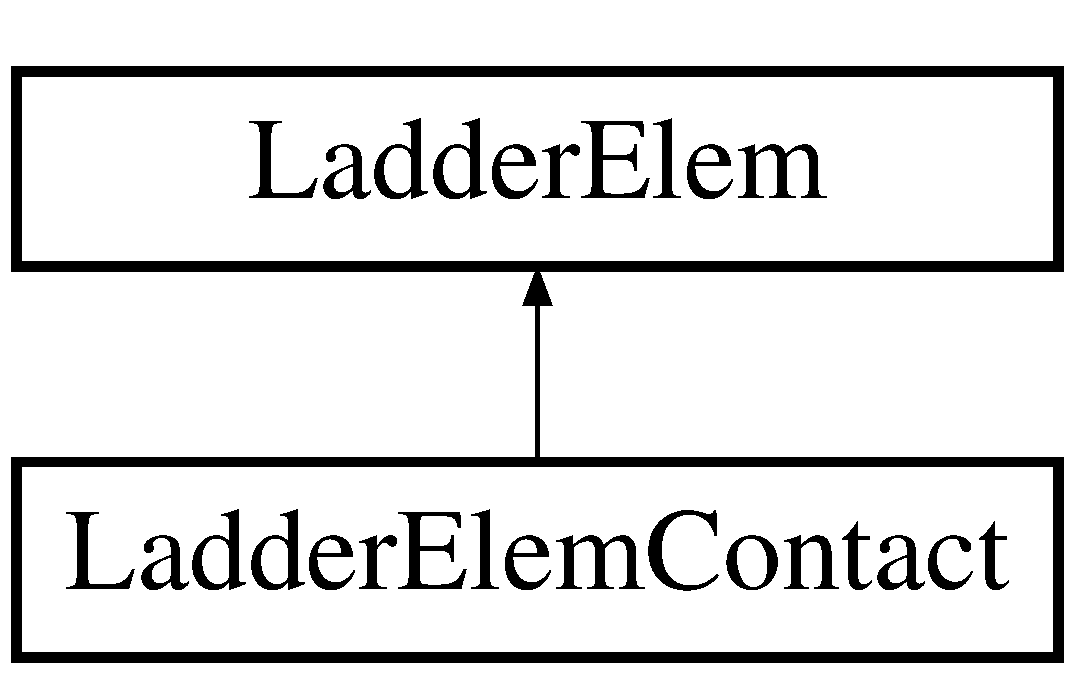
\includegraphics[height=2.000000cm]{class_ladder_elem_contact}
\end{center}
\end{figure}
\subsection*{Public Member Functions}
\begin{DoxyCompactItemize}
\item 
\hypertarget{class_ladder_elem_contact_aa5351f083bfd1e7c9c57203e05b0f81d}{{\bfseries Ladder\-Elem\-Contact} (\hyperlink{class_ladder_diagram}{Ladder\-Diagram} $\ast$diagram)}\label{class_ladder_elem_contact_aa5351f083bfd1e7c9c57203e05b0f81d}

\item 
\hypertarget{class_ladder_elem_contact_a71e5cd4d620a52267e7e8c639285c2de}{pair$<$ string, string $>$ {\bfseries Draw\-T\-X\-T} (void)}\label{class_ladder_elem_contact_a71e5cd4d620a52267e7e8c639285c2de}

\item 
\hypertarget{class_ladder_elem_contact_a7bafad9b444699d0547966751c6340c7}{bool {\bfseries Draw\-G\-U\-I} (bool powered\-Before, void $\ast$data)}\label{class_ladder_elem_contact_a7bafad9b444699d0547966751c6340c7}

\item 
\hypertarget{class_ladder_elem_contact_a7ff726a612c42daabfdd7f323beaeeb0}{bool {\bfseries Show\-Dialog} (\hyperlink{struct_ladder_context}{Ladder\-Context} context)}\label{class_ladder_elem_contact_a7ff726a612c42daabfdd7f323beaeeb0}

\item 
\hypertarget{class_ladder_elem_contact_af15149b1f93090b7219ddff4ee794d12}{bool {\bfseries internal\-Generate\-Int\-Code} (\hyperlink{class_int_code}{Int\-Code} \&ic)}\label{class_ladder_elem_contact_af15149b1f93090b7219ddff4ee794d12}

\item 
\hypertarget{class_ladder_elem_contact_a94a7de0878a167d4933cf3cf92bd2545}{void $\ast$ {\bfseries get\-Properties} (void)}\label{class_ladder_elem_contact_a94a7de0878a167d4933cf3cf92bd2545}

\item 
\hypertarget{class_ladder_elem_contact_aec9b770a27cf6cb905a6ee21541ee2a9}{bool {\bfseries Can\-Insert} (\hyperlink{struct_ladder_context}{Ladder\-Context} context)}\label{class_ladder_elem_contact_aec9b770a27cf6cb905a6ee21541ee2a9}

\item 
\hypertarget{class_ladder_elem_contact_a284ae27d3862a9c455366c1eef7855bd}{void {\bfseries do\-Post\-Insert} (void)}\label{class_ladder_elem_contact_a284ae27d3862a9c455366c1eef7855bd}

\item 
\hypertarget{class_ladder_elem_contact_ad75a7203c2643ebc876b117f6fa528a5}{void {\bfseries do\-Post\-Remove} (void)}\label{class_ladder_elem_contact_ad75a7203c2643ebc876b117f6fa528a5}

\item 
\hypertarget{class_ladder_elem_contact_a3b107a39d455d3ac0f14a8c979b2d193}{int {\bfseries get\-Width\-T\-X\-T} (void)}\label{class_ladder_elem_contact_a3b107a39d455d3ac0f14a8c979b2d193}

\item 
\hypertarget{class_ladder_elem_contact_af169ccfe9137370c6de516667fbdb2f6}{\hyperlink{class_ladder_elem}{Ladder\-Elem} $\ast$ {\bfseries Clone} (\hyperlink{class_ladder_diagram}{Ladder\-Diagram} $\ast$diagram)}\label{class_ladder_elem_contact_af169ccfe9137370c6de516667fbdb2f6}

\item 
\hypertarget{class_ladder_elem_contact_a06270fce67d6c8cded4031e5c14ffc0a}{bool {\bfseries accept\-I\-O} (unsigned long id, e\-Type type)}\label{class_ladder_elem_contact_a06270fce67d6c8cded4031e5c14ffc0a}

\item 
\hypertarget{class_ladder_elem_contact_a6a955e3ab25cc3a79dbe9a165d2fb0ad}{void {\bfseries update\-I\-O} (\hyperlink{class_ladder_diagram}{Ladder\-Diagram} $\ast$owner, bool is\-Discard)}\label{class_ladder_elem_contact_a6a955e3ab25cc3a79dbe9a165d2fb0ad}

\item 
\hypertarget{class_ladder_elem_contact_a0df03cf19201c47d5504c7360753ea32}{e\-Type {\bfseries get\-Allowed\-Type\-I\-O} (unsigned long id)}\label{class_ladder_elem_contact_a0df03cf19201c47d5504c7360753ea32}

\item 
\hypertarget{class_ladder_elem_contact_ae4efa154d4d98212995e49505c53983e}{int {\bfseries Search\-And\-Replace} (unsigned long id\-Search, string s\-New\-Text, bool is\-Replace)}\label{class_ladder_elem_contact_ae4efa154d4d98212995e49505c53983e}

\item 
\hypertarget{class_ladder_elem_contact_a0462ecb3b3efaee813e0e1fffc3e408a}{bool {\bfseries internal\-Do\-Undo\-Redo} (bool Is\-Undo, bool is\-Discard, \hyperlink{struct_undo_redo_action}{Undo\-Redo\-Action} \&action)}\label{class_ladder_elem_contact_a0462ecb3b3efaee813e0e1fffc3e408a}

\end{DoxyCompactItemize}
\subsection*{Additional Inherited Members}


The documentation for this class was generated from the following files\-:\begin{DoxyCompactItemize}
\item 
F\-:/\-S\-V\-N/\-P\-O\-P\-Tools/Ladder\-Objects.\-h\item 
F\-:/\-S\-V\-N/\-P\-O\-P\-Tools/Ladder\-G\-U\-I.\-cpp\item 
F\-:/\-S\-V\-N/\-P\-O\-P\-Tools/Ladder\-Objects.\-cpp\end{DoxyCompactItemize}

\hypertarget{struct_ladder_elem_contact_prop}{\section{Ladder\-Elem\-Contact\-Prop Struct Reference}
\label{struct_ladder_elem_contact_prop}\index{Ladder\-Elem\-Contact\-Prop@{Ladder\-Elem\-Contact\-Prop}}
}
\subsection*{Public Attributes}
\begin{DoxyCompactItemize}
\item 
\hypertarget{struct_ladder_elem_contact_prop_a22b751fc26aa82b72a135d2aac4d2599}{bool {\bfseries negated}}\label{struct_ladder_elem_contact_prop_a22b751fc26aa82b72a135d2aac4d2599}

\item 
\hypertarget{struct_ladder_elem_contact_prop_a6e564792cc6d62a2ec1f6657d69060ad}{pair$<$ unsigned long, int $>$ {\bfseries id\-Name}}\label{struct_ladder_elem_contact_prop_a6e564792cc6d62a2ec1f6657d69060ad}

\end{DoxyCompactItemize}


The documentation for this struct was generated from the following file\-:\begin{DoxyCompactItemize}
\item 
F\-:/\-S\-V\-N/\-P\-O\-P\-Tools/Ladder\-Objects.\-h\end{DoxyCompactItemize}

\hypertarget{class_ladder_elem_counter}{\section{Ladder\-Elem\-Counter Class Reference}
\label{class_ladder_elem_counter}\index{Ladder\-Elem\-Counter@{Ladder\-Elem\-Counter}}
}
Inheritance diagram for Ladder\-Elem\-Counter\-:\begin{figure}[H]
\begin{center}
\leavevmode
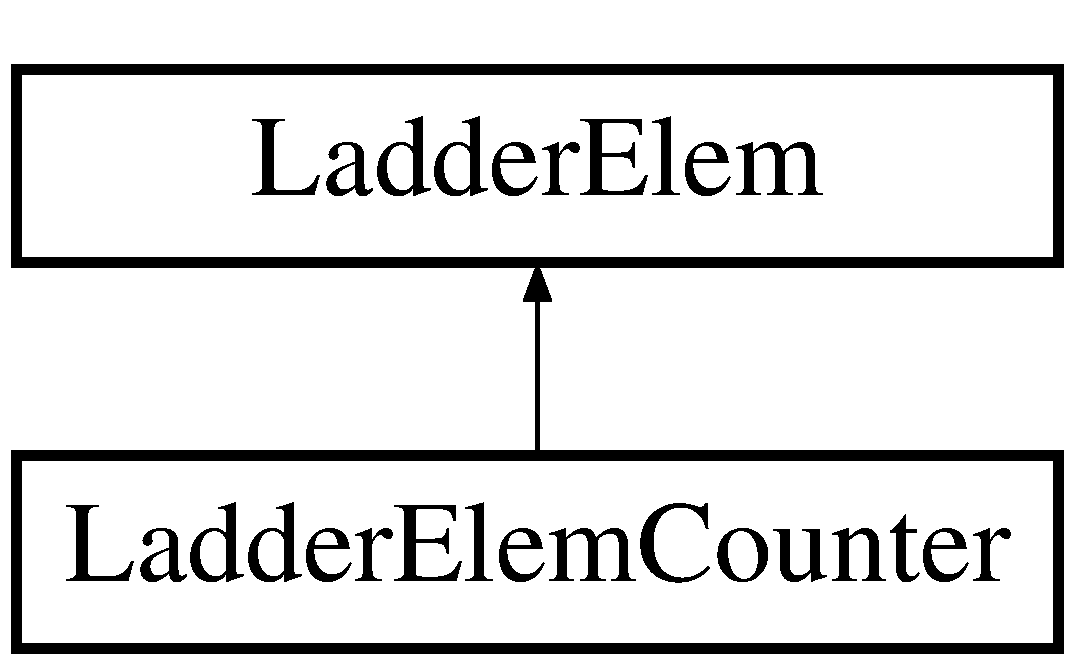
\includegraphics[height=2.000000cm]{class_ladder_elem_counter}
\end{center}
\end{figure}
\subsection*{Public Member Functions}
\begin{DoxyCompactItemize}
\item 
\hypertarget{class_ladder_elem_counter_a8c4fbb3767980abde81e159f0c8f5f48}{{\bfseries Ladder\-Elem\-Counter} (\hyperlink{class_ladder_diagram}{Ladder\-Diagram} $\ast$diagram, int which)}\label{class_ladder_elem_counter_a8c4fbb3767980abde81e159f0c8f5f48}

\item 
\hypertarget{class_ladder_elem_counter_a2796b6525c346b7f6d556e7b9c697faa}{pair$<$ string, string $>$ {\bfseries Draw\-T\-X\-T} (void)}\label{class_ladder_elem_counter_a2796b6525c346b7f6d556e7b9c697faa}

\item 
\hypertarget{class_ladder_elem_counter_ae593472f1021d3b51f2dbdc3e401eab4}{bool {\bfseries Draw\-G\-U\-I} (bool powered\-Before, void $\ast$data)}\label{class_ladder_elem_counter_ae593472f1021d3b51f2dbdc3e401eab4}

\item 
\hypertarget{class_ladder_elem_counter_aa9599ec16c2db266f40e3da5a12709ef}{bool {\bfseries Show\-Dialog} (\hyperlink{struct_ladder_context}{Ladder\-Context} context)}\label{class_ladder_elem_counter_aa9599ec16c2db266f40e3da5a12709ef}

\item 
\hypertarget{class_ladder_elem_counter_a3706168df65c8392e03bbacba57b6544}{bool {\bfseries internal\-Generate\-Int\-Code} (\hyperlink{class_int_code}{Int\-Code} \&ic)}\label{class_ladder_elem_counter_a3706168df65c8392e03bbacba57b6544}

\item 
\hypertarget{class_ladder_elem_counter_a7d6eb5b4b91f67bdd6e7bab8bf3feb84}{void $\ast$ {\bfseries get\-Properties} (void)}\label{class_ladder_elem_counter_a7d6eb5b4b91f67bdd6e7bab8bf3feb84}

\item 
\hypertarget{class_ladder_elem_counter_a2baf2b94e2ac2a2eb7102fad244f0986}{bool {\bfseries Can\-Insert} (\hyperlink{struct_ladder_context}{Ladder\-Context} context)}\label{class_ladder_elem_counter_a2baf2b94e2ac2a2eb7102fad244f0986}

\item 
\hypertarget{class_ladder_elem_counter_a5c3cf928e49af958077ed23c76650596}{void {\bfseries do\-Post\-Insert} (void)}\label{class_ladder_elem_counter_a5c3cf928e49af958077ed23c76650596}

\item 
\hypertarget{class_ladder_elem_counter_aaa9c956f817d4b703486606a1ac143ec}{void {\bfseries do\-Post\-Remove} (void)}\label{class_ladder_elem_counter_aaa9c956f817d4b703486606a1ac143ec}

\item 
\hypertarget{class_ladder_elem_counter_a67f8e18da40b5c519e4d70008f0eb1e4}{int {\bfseries get\-Width\-T\-X\-T} (void)}\label{class_ladder_elem_counter_a67f8e18da40b5c519e4d70008f0eb1e4}

\item 
\hypertarget{class_ladder_elem_counter_ab2b88eafe091f32cb5a6191a9e203427}{\hyperlink{class_ladder_elem}{Ladder\-Elem} $\ast$ {\bfseries Clone} (\hyperlink{class_ladder_diagram}{Ladder\-Diagram} $\ast$diagram)}\label{class_ladder_elem_counter_ab2b88eafe091f32cb5a6191a9e203427}

\item 
\hypertarget{class_ladder_elem_counter_a5d8c23aebd380ac8661efe6bc67b5504}{bool {\bfseries accept\-I\-O} (unsigned long id, e\-Type type)}\label{class_ladder_elem_counter_a5d8c23aebd380ac8661efe6bc67b5504}

\item 
\hypertarget{class_ladder_elem_counter_a31d814265b55bb27b52716f8f05082ea}{void {\bfseries update\-I\-O} (\hyperlink{class_ladder_diagram}{Ladder\-Diagram} $\ast$owner, bool is\-Discard)}\label{class_ladder_elem_counter_a31d814265b55bb27b52716f8f05082ea}

\item 
\hypertarget{class_ladder_elem_counter_a61f220663f615f824ada1222eeed5b99}{e\-Type {\bfseries get\-Allowed\-Type\-I\-O} (unsigned long id)}\label{class_ladder_elem_counter_a61f220663f615f824ada1222eeed5b99}

\item 
\hypertarget{class_ladder_elem_counter_a15d482409b1c2611c70977f8540a3fdf}{int {\bfseries Search\-And\-Replace} (unsigned long id\-Search, string s\-New\-Text, bool is\-Replace)}\label{class_ladder_elem_counter_a15d482409b1c2611c70977f8540a3fdf}

\item 
\hypertarget{class_ladder_elem_counter_a35296b24285986b385cdff8853b8266e}{bool {\bfseries internal\-Do\-Undo\-Redo} (bool Is\-Undo, bool is\-Discard, \hyperlink{struct_undo_redo_action}{Undo\-Redo\-Action} \&action)}\label{class_ladder_elem_counter_a35296b24285986b385cdff8853b8266e}

\end{DoxyCompactItemize}
\subsection*{Additional Inherited Members}


The documentation for this class was generated from the following files\-:\begin{DoxyCompactItemize}
\item 
F\-:/\-S\-V\-N/\-P\-O\-P\-Tools/Ladder\-Objects.\-h\item 
F\-:/\-S\-V\-N/\-P\-O\-P\-Tools/Ladder\-G\-U\-I.\-cpp\item 
F\-:/\-S\-V\-N/\-P\-O\-P\-Tools/Ladder\-Objects.\-cpp\end{DoxyCompactItemize}

\hypertarget{struct_ladder_elem_counter_prop}{\section{Ladder\-Elem\-Counter\-Prop Struct Reference}
\label{struct_ladder_elem_counter_prop}\index{Ladder\-Elem\-Counter\-Prop@{Ladder\-Elem\-Counter\-Prop}}
}
\subsection*{Public Attributes}
\begin{DoxyCompactItemize}
\item 
\hypertarget{struct_ladder_elem_counter_prop_a7452aa6c2cd012ccd39a96226c87cf8d}{pair$<$ unsigned long, int $>$ {\bfseries id\-Name}}\label{struct_ladder_elem_counter_prop_a7452aa6c2cd012ccd39a96226c87cf8d}

\item 
\hypertarget{struct_ladder_elem_counter_prop_aba0831f8b7153d1f2c316915c4694a4b}{int {\bfseries max}}\label{struct_ladder_elem_counter_prop_aba0831f8b7153d1f2c316915c4694a4b}

\end{DoxyCompactItemize}


The documentation for this struct was generated from the following file\-:\begin{DoxyCompactItemize}
\item 
F\-:/\-S\-V\-N/\-P\-O\-P\-Tools/Ladder\-Objects.\-h\end{DoxyCompactItemize}

\hypertarget{class_ladder_elem_fmt_string}{\section{Ladder\-Elem\-Fmt\-String Class Reference}
\label{class_ladder_elem_fmt_string}\index{Ladder\-Elem\-Fmt\-String@{Ladder\-Elem\-Fmt\-String}}
}
Inheritance diagram for Ladder\-Elem\-Fmt\-String\-:\begin{figure}[H]
\begin{center}
\leavevmode
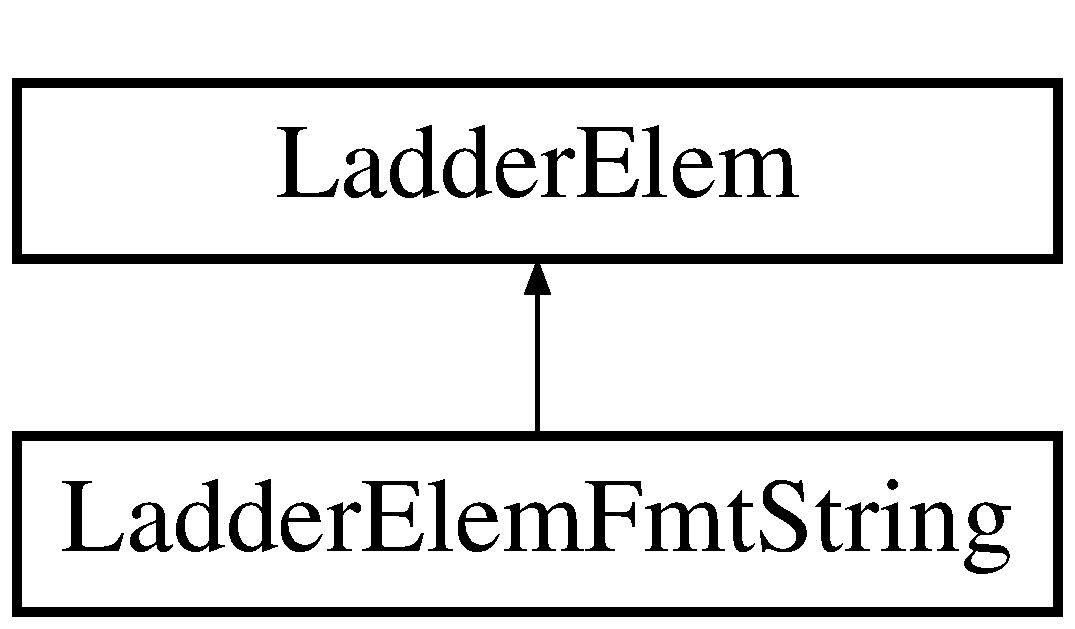
\includegraphics[height=2.000000cm]{class_ladder_elem_fmt_string}
\end{center}
\end{figure}
\subsection*{Public Member Functions}
\begin{DoxyCompactItemize}
\item 
\hypertarget{class_ladder_elem_fmt_string_afce76ad66b7b3997dc58155f837e608e}{{\bfseries Ladder\-Elem\-Fmt\-String} (\hyperlink{class_ladder_diagram}{Ladder\-Diagram} $\ast$diagram, int which)}\label{class_ladder_elem_fmt_string_afce76ad66b7b3997dc58155f837e608e}

\item 
\hypertarget{class_ladder_elem_fmt_string_a347a252ee6c1925b7e69bd9f6bfa835a}{pair$<$ string, string $>$ {\bfseries Draw\-T\-X\-T} (void)}\label{class_ladder_elem_fmt_string_a347a252ee6c1925b7e69bd9f6bfa835a}

\item 
\hypertarget{class_ladder_elem_fmt_string_ac96ca326ed22c44cf195409392ca7fdb}{bool {\bfseries Draw\-G\-U\-I} (bool powered\-Before, void $\ast$data)}\label{class_ladder_elem_fmt_string_ac96ca326ed22c44cf195409392ca7fdb}

\item 
\hypertarget{class_ladder_elem_fmt_string_a1b75a6644f771b4781c4adca3511d1f7}{bool {\bfseries Show\-Dialog} (\hyperlink{struct_ladder_context}{Ladder\-Context} context)}\label{class_ladder_elem_fmt_string_a1b75a6644f771b4781c4adca3511d1f7}

\item 
\hypertarget{class_ladder_elem_fmt_string_a979f8367db6db293792ee55c700b5a0e}{bool {\bfseries internal\-Generate\-Int\-Code} (\hyperlink{class_int_code}{Int\-Code} \&ic)}\label{class_ladder_elem_fmt_string_a979f8367db6db293792ee55c700b5a0e}

\item 
\hypertarget{class_ladder_elem_fmt_string_a715b558fdae5df2c5f5c0ae84c3a0c3d}{void $\ast$ {\bfseries get\-Properties} (void)}\label{class_ladder_elem_fmt_string_a715b558fdae5df2c5f5c0ae84c3a0c3d}

\item 
\hypertarget{class_ladder_elem_fmt_string_aad531e7418f473821cf13d41290bc9ad}{bool {\bfseries Can\-Insert} (\hyperlink{struct_ladder_context}{Ladder\-Context} context)}\label{class_ladder_elem_fmt_string_aad531e7418f473821cf13d41290bc9ad}

\item 
\hypertarget{class_ladder_elem_fmt_string_ab5d3be7a614e9bfbf369c659ef7153b5}{void {\bfseries do\-Post\-Insert} (void)}\label{class_ladder_elem_fmt_string_ab5d3be7a614e9bfbf369c659ef7153b5}

\item 
\hypertarget{class_ladder_elem_fmt_string_a966ac616e53ea4486d4a5355d8794824}{void {\bfseries do\-Post\-Remove} (void)}\label{class_ladder_elem_fmt_string_a966ac616e53ea4486d4a5355d8794824}

\item 
\hypertarget{class_ladder_elem_fmt_string_a83bb38e1a1c27065bb85424b8373b359}{int {\bfseries get\-Width\-T\-X\-T} (void)}\label{class_ladder_elem_fmt_string_a83bb38e1a1c27065bb85424b8373b359}

\item 
\hypertarget{class_ladder_elem_fmt_string_ac4ab153d69edbc04333c9a5b6ad2f803}{\hyperlink{class_ladder_elem}{Ladder\-Elem} $\ast$ {\bfseries Clone} (\hyperlink{class_ladder_diagram}{Ladder\-Diagram} $\ast$diagram)}\label{class_ladder_elem_fmt_string_ac4ab153d69edbc04333c9a5b6ad2f803}

\item 
\hypertarget{class_ladder_elem_fmt_string_ae873509eab97051d49b601f04da415a9}{bool {\bfseries accept\-I\-O} (unsigned long id, e\-Type type)}\label{class_ladder_elem_fmt_string_ae873509eab97051d49b601f04da415a9}

\item 
\hypertarget{class_ladder_elem_fmt_string_ab670e03e2b4769cc95c636f6d1605464}{void {\bfseries update\-I\-O} (\hyperlink{class_ladder_diagram}{Ladder\-Diagram} $\ast$owner, bool is\-Discard)}\label{class_ladder_elem_fmt_string_ab670e03e2b4769cc95c636f6d1605464}

\item 
\hypertarget{class_ladder_elem_fmt_string_a20dc73e2572aa0ea099fc0223bc83d3c}{e\-Type {\bfseries get\-Allowed\-Type\-I\-O} (unsigned long id)}\label{class_ladder_elem_fmt_string_a20dc73e2572aa0ea099fc0223bc83d3c}

\item 
\hypertarget{class_ladder_elem_fmt_string_a3cb41922921db611b1f49169af78fc91}{int {\bfseries Search\-And\-Replace} (unsigned long id\-Search, string s\-New\-Text, bool is\-Replace)}\label{class_ladder_elem_fmt_string_a3cb41922921db611b1f49169af78fc91}

\item 
\hypertarget{class_ladder_elem_fmt_string_aa6b6617c2da7037c95770a172b244f18}{bool {\bfseries internal\-Do\-Undo\-Redo} (bool Is\-Undo, bool is\-Discard, \hyperlink{struct_undo_redo_action}{Undo\-Redo\-Action} \&action)}\label{class_ladder_elem_fmt_string_aa6b6617c2da7037c95770a172b244f18}

\end{DoxyCompactItemize}
\subsection*{Additional Inherited Members}


The documentation for this class was generated from the following files\-:\begin{DoxyCompactItemize}
\item 
F\-:/\-S\-V\-N/\-P\-O\-P\-Tools/Ladder\-Objects.\-h\item 
F\-:/\-S\-V\-N/\-P\-O\-P\-Tools/Ladder\-G\-U\-I.\-cpp\item 
F\-:/\-S\-V\-N/\-P\-O\-P\-Tools/Ladder\-Objects.\-cpp\end{DoxyCompactItemize}

\hypertarget{struct_ladder_elem_fmt_string_prop}{\section{Ladder\-Elem\-Fmt\-String\-Prop Struct Reference}
\label{struct_ladder_elem_fmt_string_prop}\index{Ladder\-Elem\-Fmt\-String\-Prop@{Ladder\-Elem\-Fmt\-String\-Prop}}
}
\subsection*{Public Attributes}
\begin{DoxyCompactItemize}
\item 
\hypertarget{struct_ladder_elem_fmt_string_prop_a9a08c3dc9cf821c591284451e0123841}{pair$<$ unsigned long, int $>$ {\bfseries id\-Var}}\label{struct_ladder_elem_fmt_string_prop_a9a08c3dc9cf821c591284451e0123841}

\item 
\hypertarget{struct_ladder_elem_fmt_string_prop_ad90af2417d11c46db937e03a20087624}{string {\bfseries txt}}\label{struct_ladder_elem_fmt_string_prop_ad90af2417d11c46db937e03a20087624}

\end{DoxyCompactItemize}


The documentation for this struct was generated from the following file\-:\begin{DoxyCompactItemize}
\item 
F\-:/\-S\-V\-N/\-P\-O\-P\-Tools/Ladder\-Objects.\-h\end{DoxyCompactItemize}

\hypertarget{class_ladder_elem_l_u_t}{\section{Ladder\-Elem\-L\-U\-T Class Reference}
\label{class_ladder_elem_l_u_t}\index{Ladder\-Elem\-L\-U\-T@{Ladder\-Elem\-L\-U\-T}}
}
Inheritance diagram for Ladder\-Elem\-L\-U\-T\-:\begin{figure}[H]
\begin{center}
\leavevmode
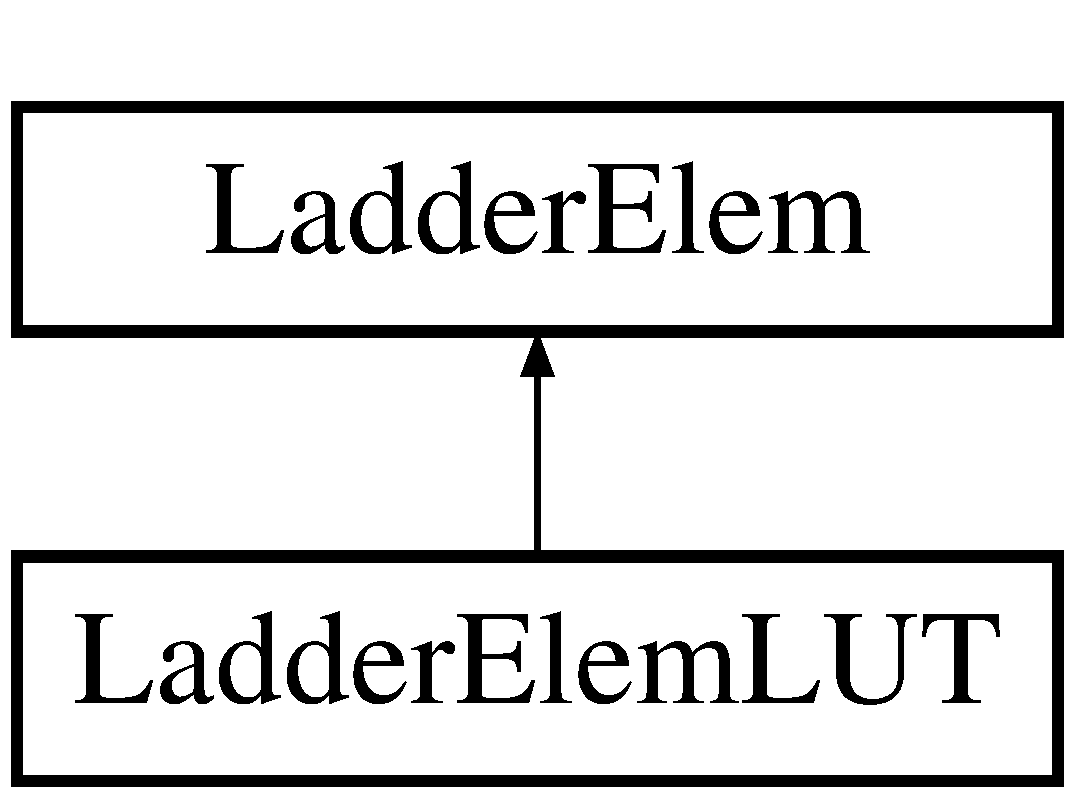
\includegraphics[height=2.000000cm]{class_ladder_elem_l_u_t}
\end{center}
\end{figure}
\subsection*{Public Member Functions}
\begin{DoxyCompactItemize}
\item 
\hypertarget{class_ladder_elem_l_u_t_a69566c6dfa6a190545bbe69262cfd16f}{{\bfseries Ladder\-Elem\-L\-U\-T} (\hyperlink{class_ladder_diagram}{Ladder\-Diagram} $\ast$diagram)}\label{class_ladder_elem_l_u_t_a69566c6dfa6a190545bbe69262cfd16f}

\item 
\hypertarget{class_ladder_elem_l_u_t_adf99aeac97bc0ea67537ff34bac6b676}{pair$<$ string, string $>$ {\bfseries Draw\-T\-X\-T} (void)}\label{class_ladder_elem_l_u_t_adf99aeac97bc0ea67537ff34bac6b676}

\item 
\hypertarget{class_ladder_elem_l_u_t_a62604b9a453829399a33190c28aa28ec}{bool {\bfseries Draw\-G\-U\-I} (bool powered\-Before, void $\ast$data)}\label{class_ladder_elem_l_u_t_a62604b9a453829399a33190c28aa28ec}

\item 
\hypertarget{class_ladder_elem_l_u_t_ae989efcd4e1b1e720fed9fc2136843e1}{bool {\bfseries Show\-Dialog} (\hyperlink{struct_ladder_context}{Ladder\-Context} context)}\label{class_ladder_elem_l_u_t_ae989efcd4e1b1e720fed9fc2136843e1}

\item 
\hypertarget{class_ladder_elem_l_u_t_a1b0fea971029e6c8f46a2e459a8ed75f}{bool {\bfseries internal\-Generate\-Int\-Code} (\hyperlink{class_int_code}{Int\-Code} \&ic)}\label{class_ladder_elem_l_u_t_a1b0fea971029e6c8f46a2e459a8ed75f}

\item 
\hypertarget{class_ladder_elem_l_u_t_a81d220ea3d402f3e64a1b235c21a9f32}{void $\ast$ {\bfseries get\-Properties} (void)}\label{class_ladder_elem_l_u_t_a81d220ea3d402f3e64a1b235c21a9f32}

\item 
\hypertarget{class_ladder_elem_l_u_t_a145d30b441795c0d6a29a71c800764a9}{bool {\bfseries Can\-Insert} (\hyperlink{struct_ladder_context}{Ladder\-Context} context)}\label{class_ladder_elem_l_u_t_a145d30b441795c0d6a29a71c800764a9}

\item 
\hypertarget{class_ladder_elem_l_u_t_ae6973942ae6a47c34a445190a5e4fc6d}{void {\bfseries do\-Post\-Insert} (void)}\label{class_ladder_elem_l_u_t_ae6973942ae6a47c34a445190a5e4fc6d}

\item 
\hypertarget{class_ladder_elem_l_u_t_a8a597c75f45b5df068afc7b07ff14eda}{void {\bfseries do\-Post\-Remove} (void)}\label{class_ladder_elem_l_u_t_a8a597c75f45b5df068afc7b07ff14eda}

\item 
\hypertarget{class_ladder_elem_l_u_t_afa4d8679572f2a4d76ef907d16717814}{int {\bfseries get\-Width\-T\-X\-T} (void)}\label{class_ladder_elem_l_u_t_afa4d8679572f2a4d76ef907d16717814}

\item 
\hypertarget{class_ladder_elem_l_u_t_aea23111ce8ed4b380edf19ded1432ef4}{\hyperlink{class_ladder_elem}{Ladder\-Elem} $\ast$ {\bfseries Clone} (\hyperlink{class_ladder_diagram}{Ladder\-Diagram} $\ast$diagram)}\label{class_ladder_elem_l_u_t_aea23111ce8ed4b380edf19ded1432ef4}

\item 
\hypertarget{class_ladder_elem_l_u_t_adc27ac7e3b707039ca21318e2f1cd185}{bool {\bfseries accept\-I\-O} (unsigned long id, e\-Type type)}\label{class_ladder_elem_l_u_t_adc27ac7e3b707039ca21318e2f1cd185}

\item 
\hypertarget{class_ladder_elem_l_u_t_ae6b693857ea412da46970891fd1e496d}{void {\bfseries update\-I\-O} (\hyperlink{class_ladder_diagram}{Ladder\-Diagram} $\ast$owner, bool is\-Discard)}\label{class_ladder_elem_l_u_t_ae6b693857ea412da46970891fd1e496d}

\item 
\hypertarget{class_ladder_elem_l_u_t_a446cea21ccfc32bf7943280a4c5b4715}{e\-Type {\bfseries get\-Allowed\-Type\-I\-O} (unsigned long id)}\label{class_ladder_elem_l_u_t_a446cea21ccfc32bf7943280a4c5b4715}

\item 
\hypertarget{class_ladder_elem_l_u_t_ac6c7ae42c41bfe873cd91e6e5188fcee}{int {\bfseries Search\-And\-Replace} (unsigned long id\-Search, string s\-New\-Text, bool is\-Replace)}\label{class_ladder_elem_l_u_t_ac6c7ae42c41bfe873cd91e6e5188fcee}

\item 
\hypertarget{class_ladder_elem_l_u_t_a6e86d657f459ba8e5f0afd568520d3b7}{bool {\bfseries internal\-Do\-Undo\-Redo} (bool Is\-Undo, bool is\-Discard, \hyperlink{struct_undo_redo_action}{Undo\-Redo\-Action} \&action)}\label{class_ladder_elem_l_u_t_a6e86d657f459ba8e5f0afd568520d3b7}

\end{DoxyCompactItemize}
\subsection*{Additional Inherited Members}


The documentation for this class was generated from the following files\-:\begin{DoxyCompactItemize}
\item 
F\-:/\-S\-V\-N/\-P\-O\-P\-Tools/Ladder\-Objects.\-h\item 
F\-:/\-S\-V\-N/\-P\-O\-P\-Tools/Ladder\-G\-U\-I.\-cpp\item 
F\-:/\-S\-V\-N/\-P\-O\-P\-Tools/Ladder\-Objects.\-cpp\end{DoxyCompactItemize}

\hypertarget{struct_ladder_elem_l_u_t_prop}{\section{Ladder\-Elem\-L\-U\-T\-Prop Struct Reference}
\label{struct_ladder_elem_l_u_t_prop}\index{Ladder\-Elem\-L\-U\-T\-Prop@{Ladder\-Elem\-L\-U\-T\-Prop}}
}
\subsection*{Public Attributes}
\begin{DoxyCompactItemize}
\item 
\hypertarget{struct_ladder_elem_l_u_t_prop_a42058a10e7f3bcb956625e7ac8db3dd0}{pair$<$ unsigned long, int $>$ {\bfseries id\-Dest}}\label{struct_ladder_elem_l_u_t_prop_a42058a10e7f3bcb956625e7ac8db3dd0}

\item 
\hypertarget{struct_ladder_elem_l_u_t_prop_acb243816bc598c60904dfaffd42f3091}{pair$<$ unsigned long, int $>$ {\bfseries id\-Index}}\label{struct_ladder_elem_l_u_t_prop_acb243816bc598c60904dfaffd42f3091}

\item 
\hypertarget{struct_ladder_elem_l_u_t_prop_a693d57b799493682987890fc09ae561c}{int {\bfseries count}}\label{struct_ladder_elem_l_u_t_prop_a693d57b799493682987890fc09ae561c}

\item 
\hypertarget{struct_ladder_elem_l_u_t_prop_aba37f92334c49012369c0c0c2193a954}{bool {\bfseries edit\-As\-String}}\label{struct_ladder_elem_l_u_t_prop_aba37f92334c49012369c0c0c2193a954}

\item 
\hypertarget{struct_ladder_elem_l_u_t_prop_ae77940f16a3f6c54a781e7db8950a19b}{array$<$ long, \\*
M\-A\-X\-\_\-\-L\-O\-O\-K\-\_\-\-U\-P\-\_\-\-T\-A\-B\-L\-E\-\_\-\-L\-E\-N $>$ {\bfseries vals}}\label{struct_ladder_elem_l_u_t_prop_ae77940f16a3f6c54a781e7db8950a19b}

\end{DoxyCompactItemize}


The documentation for this struct was generated from the following file\-:\begin{DoxyCompactItemize}
\item 
F\-:/\-S\-V\-N/\-P\-O\-P\-Tools/Ladder\-Objects.\-h\end{DoxyCompactItemize}

\hypertarget{class_ladder_elem_master_relay}{\section{Ladder\-Elem\-Master\-Relay Class Reference}
\label{class_ladder_elem_master_relay}\index{Ladder\-Elem\-Master\-Relay@{Ladder\-Elem\-Master\-Relay}}
}
Inheritance diagram for Ladder\-Elem\-Master\-Relay\-:\begin{figure}[H]
\begin{center}
\leavevmode
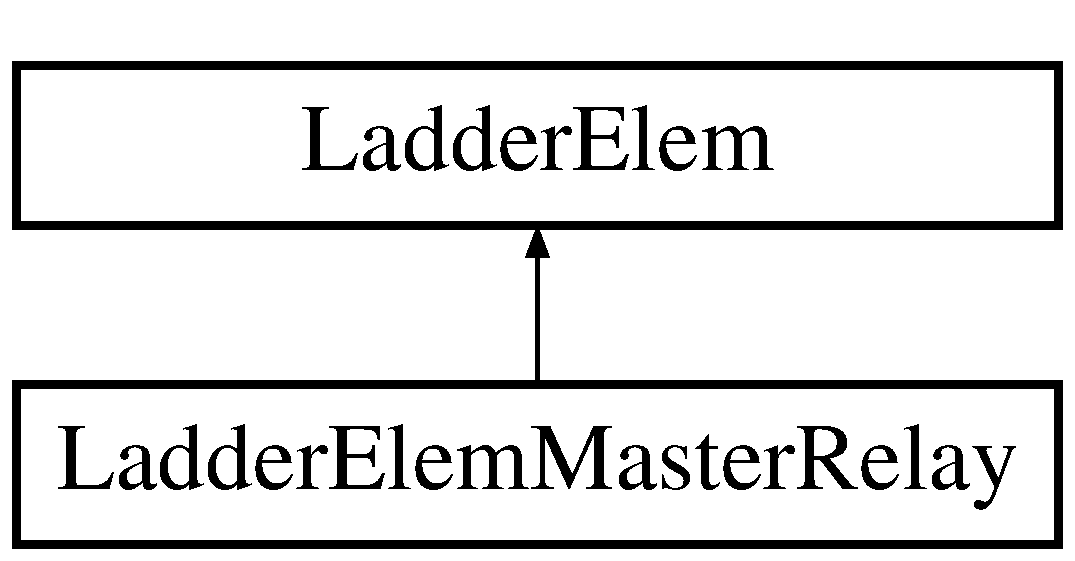
\includegraphics[height=2.000000cm]{class_ladder_elem_master_relay}
\end{center}
\end{figure}
\subsection*{Public Member Functions}
\begin{DoxyCompactItemize}
\item 
\hypertarget{class_ladder_elem_master_relay_a450e0168c3118753cb814de8f9d7df97}{{\bfseries Ladder\-Elem\-Master\-Relay} (\hyperlink{class_ladder_diagram}{Ladder\-Diagram} $\ast$diagram)}\label{class_ladder_elem_master_relay_a450e0168c3118753cb814de8f9d7df97}

\item 
\hypertarget{class_ladder_elem_master_relay_a24cd86cad80fe4e7fe0f9d11fab8e89e}{pair$<$ string, string $>$ {\bfseries Draw\-T\-X\-T} (void)}\label{class_ladder_elem_master_relay_a24cd86cad80fe4e7fe0f9d11fab8e89e}

\item 
\hypertarget{class_ladder_elem_master_relay_a989e496a2eb10cb14e7371c135a2d674}{bool {\bfseries Draw\-G\-U\-I} (bool powered\-Before, void $\ast$data)}\label{class_ladder_elem_master_relay_a989e496a2eb10cb14e7371c135a2d674}

\item 
\hypertarget{class_ladder_elem_master_relay_aa6a4be764a872a3df31e06e49af1a037}{bool {\bfseries Show\-Dialog} (\hyperlink{struct_ladder_context}{Ladder\-Context} context)}\label{class_ladder_elem_master_relay_aa6a4be764a872a3df31e06e49af1a037}

\item 
\hypertarget{class_ladder_elem_master_relay_ab730eb84a0a414e3b79ceb5c3e5468b1}{bool {\bfseries internal\-Generate\-Int\-Code} (\hyperlink{class_int_code}{Int\-Code} \&ic)}\label{class_ladder_elem_master_relay_ab730eb84a0a414e3b79ceb5c3e5468b1}

\item 
\hypertarget{class_ladder_elem_master_relay_af3cb4608e99355397478bcd78f842d5b}{void $\ast$ {\bfseries get\-Properties} (void)}\label{class_ladder_elem_master_relay_af3cb4608e99355397478bcd78f842d5b}

\item 
\hypertarget{class_ladder_elem_master_relay_a2d0a54eb80f0c244f643825e84295475}{bool {\bfseries Can\-Insert} (\hyperlink{struct_ladder_context}{Ladder\-Context} context)}\label{class_ladder_elem_master_relay_a2d0a54eb80f0c244f643825e84295475}

\item 
\hypertarget{class_ladder_elem_master_relay_aa83f2cfecc873a60ebae5fa2eb1f162b}{void {\bfseries do\-Post\-Insert} (void)}\label{class_ladder_elem_master_relay_aa83f2cfecc873a60ebae5fa2eb1f162b}

\item 
\hypertarget{class_ladder_elem_master_relay_a8ddd30f8aa62070f3422a9f45e094e37}{void {\bfseries do\-Post\-Remove} (void)}\label{class_ladder_elem_master_relay_a8ddd30f8aa62070f3422a9f45e094e37}

\item 
\hypertarget{class_ladder_elem_master_relay_a69ea67b15af982d9b4daf53974882692}{int {\bfseries get\-Width\-T\-X\-T} (void)}\label{class_ladder_elem_master_relay_a69ea67b15af982d9b4daf53974882692}

\item 
\hypertarget{class_ladder_elem_master_relay_a5a6a647c5b909817472ca2ca876ef17f}{\hyperlink{class_ladder_elem}{Ladder\-Elem} $\ast$ {\bfseries Clone} (\hyperlink{class_ladder_diagram}{Ladder\-Diagram} $\ast$diagram)}\label{class_ladder_elem_master_relay_a5a6a647c5b909817472ca2ca876ef17f}

\item 
\hypertarget{class_ladder_elem_master_relay_a8e925f39d5eb0f747761366e4648207f}{bool {\bfseries accept\-I\-O} (unsigned long id, e\-Type type)}\label{class_ladder_elem_master_relay_a8e925f39d5eb0f747761366e4648207f}

\item 
\hypertarget{class_ladder_elem_master_relay_a54c7d0685661dd16760ae16199b221d7}{void {\bfseries update\-I\-O} (\hyperlink{class_ladder_diagram}{Ladder\-Diagram} $\ast$owner, bool is\-Discard)}\label{class_ladder_elem_master_relay_a54c7d0685661dd16760ae16199b221d7}

\item 
\hypertarget{class_ladder_elem_master_relay_a28ffa17b9af9e42c85bf8e59c20492dd}{e\-Type {\bfseries get\-Allowed\-Type\-I\-O} (unsigned long id)}\label{class_ladder_elem_master_relay_a28ffa17b9af9e42c85bf8e59c20492dd}

\item 
\hypertarget{class_ladder_elem_master_relay_a8f06eabd29613ab89e83aff1176a0f4d}{int {\bfseries Search\-And\-Replace} (unsigned long id\-Search, string s\-New\-Text, bool is\-Replace)}\label{class_ladder_elem_master_relay_a8f06eabd29613ab89e83aff1176a0f4d}

\item 
\hypertarget{class_ladder_elem_master_relay_a31ed1aa5b566dd37721a210c6ef76689}{bool {\bfseries internal\-Do\-Undo\-Redo} (bool Is\-Undo, bool is\-Discard, \hyperlink{struct_undo_redo_action}{Undo\-Redo\-Action} \&action)}\label{class_ladder_elem_master_relay_a31ed1aa5b566dd37721a210c6ef76689}

\end{DoxyCompactItemize}
\subsection*{Additional Inherited Members}


The documentation for this class was generated from the following files\-:\begin{DoxyCompactItemize}
\item 
F\-:/\-S\-V\-N/\-P\-O\-P\-Tools/Ladder\-Objects.\-h\item 
F\-:/\-S\-V\-N/\-P\-O\-P\-Tools/Ladder\-G\-U\-I.\-cpp\item 
F\-:/\-S\-V\-N/\-P\-O\-P\-Tools/Ladder\-Objects.\-cpp\end{DoxyCompactItemize}

\hypertarget{class_ladder_elem_math}{\section{Ladder\-Elem\-Math Class Reference}
\label{class_ladder_elem_math}\index{Ladder\-Elem\-Math@{Ladder\-Elem\-Math}}
}
Inheritance diagram for Ladder\-Elem\-Math\-:\begin{figure}[H]
\begin{center}
\leavevmode
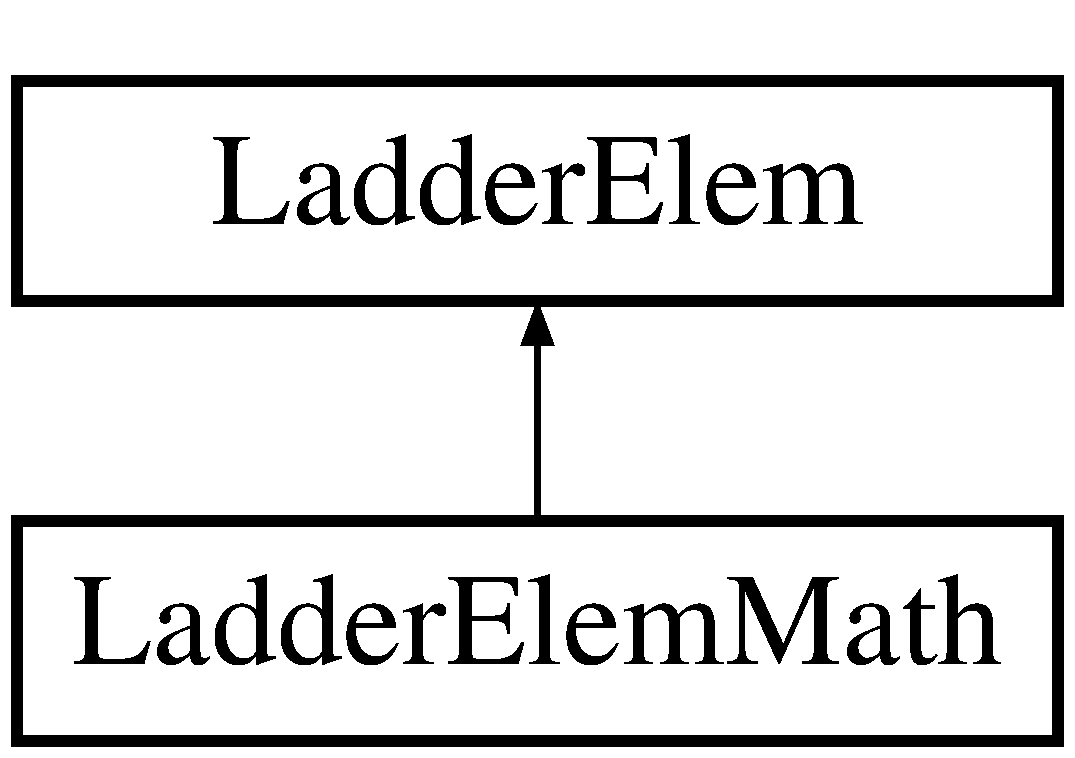
\includegraphics[height=2.000000cm]{class_ladder_elem_math}
\end{center}
\end{figure}
\subsection*{Public Member Functions}
\begin{DoxyCompactItemize}
\item 
\hypertarget{class_ladder_elem_math_a8d6a3df031c139f5e81f93d044be7a22}{{\bfseries Ladder\-Elem\-Math} (\hyperlink{class_ladder_diagram}{Ladder\-Diagram} $\ast$diagram, int which)}\label{class_ladder_elem_math_a8d6a3df031c139f5e81f93d044be7a22}

\item 
\hypertarget{class_ladder_elem_math_af7cef4469c605f9b87a322a215c8c16a}{pair$<$ string, string $>$ {\bfseries Draw\-T\-X\-T} (void)}\label{class_ladder_elem_math_af7cef4469c605f9b87a322a215c8c16a}

\item 
\hypertarget{class_ladder_elem_math_a0ddf923301b57a233e2a899f1d9187ec}{bool {\bfseries Draw\-G\-U\-I} (bool powered\-Before, void $\ast$data)}\label{class_ladder_elem_math_a0ddf923301b57a233e2a899f1d9187ec}

\item 
\hypertarget{class_ladder_elem_math_a1a8327caf04accce4242e3a90eb9d1c2}{bool {\bfseries Show\-Dialog} (\hyperlink{struct_ladder_context}{Ladder\-Context} context)}\label{class_ladder_elem_math_a1a8327caf04accce4242e3a90eb9d1c2}

\item 
\hypertarget{class_ladder_elem_math_af4a9739a663efab7a705326940c9a2da}{bool {\bfseries internal\-Generate\-Int\-Code} (\hyperlink{class_int_code}{Int\-Code} \&ic)}\label{class_ladder_elem_math_af4a9739a663efab7a705326940c9a2da}

\item 
\hypertarget{class_ladder_elem_math_a8c6bc1193cc45b86178fbc50e91c080e}{void $\ast$ {\bfseries get\-Properties} (void)}\label{class_ladder_elem_math_a8c6bc1193cc45b86178fbc50e91c080e}

\item 
\hypertarget{class_ladder_elem_math_a3551747bba8497ff08a70a43f50eabd3}{bool {\bfseries Can\-Insert} (\hyperlink{struct_ladder_context}{Ladder\-Context} context)}\label{class_ladder_elem_math_a3551747bba8497ff08a70a43f50eabd3}

\item 
\hypertarget{class_ladder_elem_math_adaf500905852a5f2936804fe6675a10e}{void {\bfseries do\-Post\-Insert} (void)}\label{class_ladder_elem_math_adaf500905852a5f2936804fe6675a10e}

\item 
\hypertarget{class_ladder_elem_math_a4b6e643b98cb5dccd9a9b98408daf9b7}{void {\bfseries do\-Post\-Remove} (void)}\label{class_ladder_elem_math_a4b6e643b98cb5dccd9a9b98408daf9b7}

\item 
\hypertarget{class_ladder_elem_math_a8d48550924dac183d9445808e99d7548}{int {\bfseries get\-Width\-T\-X\-T} (void)}\label{class_ladder_elem_math_a8d48550924dac183d9445808e99d7548}

\item 
\hypertarget{class_ladder_elem_math_ad5577271547f1335850496e7341d96b9}{\hyperlink{class_ladder_elem}{Ladder\-Elem} $\ast$ {\bfseries Clone} (\hyperlink{class_ladder_diagram}{Ladder\-Diagram} $\ast$diagram)}\label{class_ladder_elem_math_ad5577271547f1335850496e7341d96b9}

\item 
\hypertarget{class_ladder_elem_math_abc5d657de2c736adfd47f14623cd7f5c}{bool {\bfseries accept\-I\-O} (unsigned long id, e\-Type type)}\label{class_ladder_elem_math_abc5d657de2c736adfd47f14623cd7f5c}

\item 
\hypertarget{class_ladder_elem_math_a53f275c915761d323cc17285c42f7141}{void {\bfseries update\-I\-O} (\hyperlink{class_ladder_diagram}{Ladder\-Diagram} $\ast$owner, bool is\-Discard)}\label{class_ladder_elem_math_a53f275c915761d323cc17285c42f7141}

\item 
\hypertarget{class_ladder_elem_math_aa30556e55067a0d34e29ae7f69e1bc86}{e\-Type {\bfseries get\-Allowed\-Type\-I\-O} (unsigned long id)}\label{class_ladder_elem_math_aa30556e55067a0d34e29ae7f69e1bc86}

\item 
\hypertarget{class_ladder_elem_math_a86553eda815473985f74a5cd40cdbc59}{int {\bfseries Search\-And\-Replace} (unsigned long id\-Search, string s\-New\-Text, bool is\-Replace)}\label{class_ladder_elem_math_a86553eda815473985f74a5cd40cdbc59}

\item 
\hypertarget{class_ladder_elem_math_a36a4d900dbabb7d7e43d8cc8d3d15c5a}{bool {\bfseries internal\-Do\-Undo\-Redo} (bool Is\-Undo, bool is\-Discard, \hyperlink{struct_undo_redo_action}{Undo\-Redo\-Action} \&action)}\label{class_ladder_elem_math_a36a4d900dbabb7d7e43d8cc8d3d15c5a}

\end{DoxyCompactItemize}
\subsection*{Additional Inherited Members}


The documentation for this class was generated from the following files\-:\begin{DoxyCompactItemize}
\item 
F\-:/\-S\-V\-N/\-P\-O\-P\-Tools/Ladder\-Objects.\-h\item 
F\-:/\-S\-V\-N/\-P\-O\-P\-Tools/Ladder\-G\-U\-I.\-cpp\item 
F\-:/\-S\-V\-N/\-P\-O\-P\-Tools/Ladder\-Objects.\-cpp\end{DoxyCompactItemize}

\hypertarget{struct_ladder_elem_math_prop}{\section{Ladder\-Elem\-Math\-Prop Struct Reference}
\label{struct_ladder_elem_math_prop}\index{Ladder\-Elem\-Math\-Prop@{Ladder\-Elem\-Math\-Prop}}
}
\subsection*{Public Attributes}
\begin{DoxyCompactItemize}
\item 
\hypertarget{struct_ladder_elem_math_prop_a34a443fae4353db39ae5c75eace145af}{pair$<$ unsigned long, int $>$ {\bfseries id\-Op1}}\label{struct_ladder_elem_math_prop_a34a443fae4353db39ae5c75eace145af}

\item 
\hypertarget{struct_ladder_elem_math_prop_a2751dca59c72e68e81446bbc6ea87ab0}{pair$<$ unsigned long, int $>$ {\bfseries id\-Op2}}\label{struct_ladder_elem_math_prop_a2751dca59c72e68e81446bbc6ea87ab0}

\item 
\hypertarget{struct_ladder_elem_math_prop_ac985d7e9381d7767e3d348cdf774e948}{pair$<$ unsigned long, int $>$ {\bfseries id\-Dest}}\label{struct_ladder_elem_math_prop_ac985d7e9381d7767e3d348cdf774e948}

\end{DoxyCompactItemize}


The documentation for this struct was generated from the following file\-:\begin{DoxyCompactItemize}
\item 
F\-:/\-S\-V\-N/\-P\-O\-P\-Tools/Ladder\-Objects.\-h\end{DoxyCompactItemize}

\hypertarget{class_ladder_elem_mod_b_u_s}{\section{Ladder\-Elem\-Mod\-B\-U\-S Class Reference}
\label{class_ladder_elem_mod_b_u_s}\index{Ladder\-Elem\-Mod\-B\-U\-S@{Ladder\-Elem\-Mod\-B\-U\-S}}
}
Inheritance diagram for Ladder\-Elem\-Mod\-B\-U\-S\-:\begin{figure}[H]
\begin{center}
\leavevmode
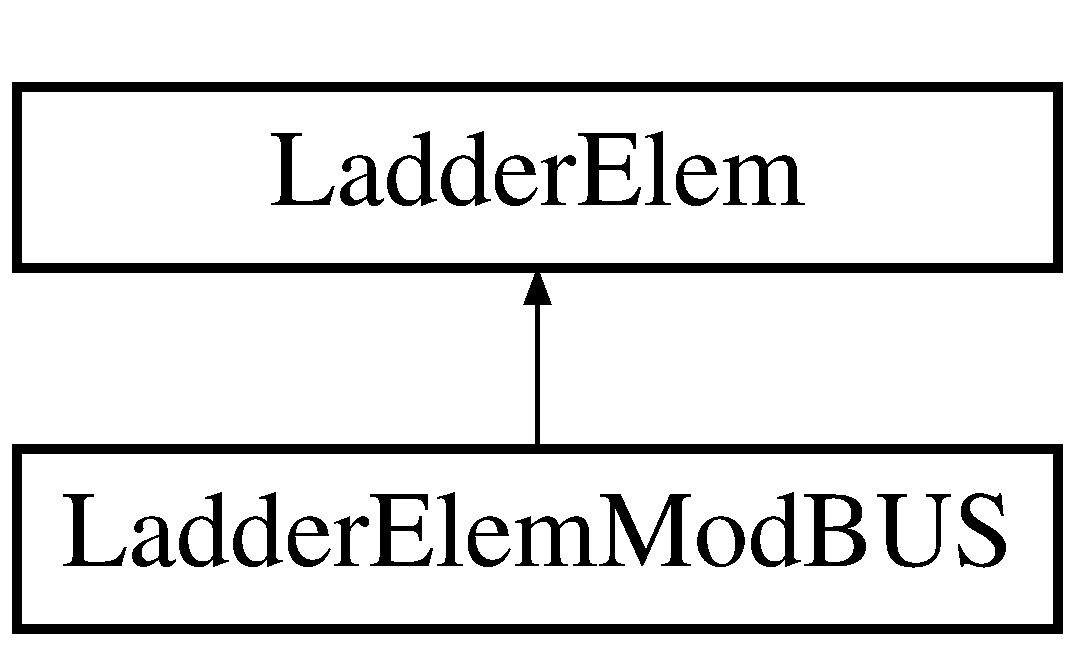
\includegraphics[height=2.000000cm]{class_ladder_elem_mod_b_u_s}
\end{center}
\end{figure}
\subsection*{Public Member Functions}
\begin{DoxyCompactItemize}
\item 
\hypertarget{class_ladder_elem_mod_b_u_s_ad4f08a6913efe55e6010d008a62bc289}{{\bfseries Ladder\-Elem\-Mod\-B\-U\-S} (\hyperlink{class_ladder_diagram}{Ladder\-Diagram} $\ast$diagram, int which)}\label{class_ladder_elem_mod_b_u_s_ad4f08a6913efe55e6010d008a62bc289}

\item 
\hypertarget{class_ladder_elem_mod_b_u_s_a5531942682b2163150dcde3bdfab297a}{pair$<$ string, string $>$ {\bfseries Draw\-T\-X\-T} (void)}\label{class_ladder_elem_mod_b_u_s_a5531942682b2163150dcde3bdfab297a}

\item 
\hypertarget{class_ladder_elem_mod_b_u_s_a4d5e8f4a14d08a5291642733da0a92fe}{bool {\bfseries Draw\-G\-U\-I} (bool powered\-Before, void $\ast$data)}\label{class_ladder_elem_mod_b_u_s_a4d5e8f4a14d08a5291642733da0a92fe}

\item 
\hypertarget{class_ladder_elem_mod_b_u_s_adb3745a6605a0d5c2851e3436e611741}{bool {\bfseries Show\-Dialog} (\hyperlink{struct_ladder_context}{Ladder\-Context} context)}\label{class_ladder_elem_mod_b_u_s_adb3745a6605a0d5c2851e3436e611741}

\item 
\hypertarget{class_ladder_elem_mod_b_u_s_af4727e8fe6e854d283a8cd35eec4d80a}{bool {\bfseries internal\-Generate\-Int\-Code} (\hyperlink{class_int_code}{Int\-Code} \&ic)}\label{class_ladder_elem_mod_b_u_s_af4727e8fe6e854d283a8cd35eec4d80a}

\item 
\hypertarget{class_ladder_elem_mod_b_u_s_a22f91b352cb5d2d9b760efed071cc9e8}{void $\ast$ {\bfseries get\-Properties} (void)}\label{class_ladder_elem_mod_b_u_s_a22f91b352cb5d2d9b760efed071cc9e8}

\item 
\hypertarget{class_ladder_elem_mod_b_u_s_ac0a9b9ae02def30158c77345682c2752}{bool {\bfseries Can\-Insert} (\hyperlink{struct_ladder_context}{Ladder\-Context} context)}\label{class_ladder_elem_mod_b_u_s_ac0a9b9ae02def30158c77345682c2752}

\item 
\hypertarget{class_ladder_elem_mod_b_u_s_a5da1d1baa3fa1bd58a8b006fb5841038}{void {\bfseries do\-Post\-Insert} (void)}\label{class_ladder_elem_mod_b_u_s_a5da1d1baa3fa1bd58a8b006fb5841038}

\item 
\hypertarget{class_ladder_elem_mod_b_u_s_a6041774d6a3e169fa7346b95b57711b0}{void {\bfseries do\-Post\-Remove} (void)}\label{class_ladder_elem_mod_b_u_s_a6041774d6a3e169fa7346b95b57711b0}

\item 
\hypertarget{class_ladder_elem_mod_b_u_s_a1196e420e5d542370b5d7f4d6be2a252}{int {\bfseries get\-Width\-T\-X\-T} (void)}\label{class_ladder_elem_mod_b_u_s_a1196e420e5d542370b5d7f4d6be2a252}

\item 
\hypertarget{class_ladder_elem_mod_b_u_s_a6686b8075fc0ec04fde8ffaa230e986d}{\hyperlink{class_ladder_elem}{Ladder\-Elem} $\ast$ {\bfseries Clone} (\hyperlink{class_ladder_diagram}{Ladder\-Diagram} $\ast$diagram)}\label{class_ladder_elem_mod_b_u_s_a6686b8075fc0ec04fde8ffaa230e986d}

\item 
\hypertarget{class_ladder_elem_mod_b_u_s_a22f4a7dfec9513c0bdf928c8204fc712}{bool {\bfseries accept\-I\-O} (unsigned long id, e\-Type type)}\label{class_ladder_elem_mod_b_u_s_a22f4a7dfec9513c0bdf928c8204fc712}

\item 
\hypertarget{class_ladder_elem_mod_b_u_s_ae2060b2626e86977a5f1a67dd42626b9}{void {\bfseries update\-I\-O} (\hyperlink{class_ladder_diagram}{Ladder\-Diagram} $\ast$owner, bool is\-Discard)}\label{class_ladder_elem_mod_b_u_s_ae2060b2626e86977a5f1a67dd42626b9}

\item 
\hypertarget{class_ladder_elem_mod_b_u_s_a1547dce8ccb99c111d94e546a430a5dd}{e\-Type {\bfseries get\-Allowed\-Type\-I\-O} (unsigned long id)}\label{class_ladder_elem_mod_b_u_s_a1547dce8ccb99c111d94e546a430a5dd}

\item 
\hypertarget{class_ladder_elem_mod_b_u_s_a2a8101db1f9d075d1d7a4ca114147177}{int {\bfseries Search\-And\-Replace} (unsigned long id\-Search, string s\-New\-Text, bool is\-Replace)}\label{class_ladder_elem_mod_b_u_s_a2a8101db1f9d075d1d7a4ca114147177}

\item 
\hypertarget{class_ladder_elem_mod_b_u_s_a0866ed8c8e56b4a7f1d5d92caaaf27ef}{bool {\bfseries internal\-Do\-Undo\-Redo} (bool Is\-Undo, bool is\-Discard, \hyperlink{struct_undo_redo_action}{Undo\-Redo\-Action} \&action)}\label{class_ladder_elem_mod_b_u_s_a0866ed8c8e56b4a7f1d5d92caaaf27ef}

\end{DoxyCompactItemize}
\subsection*{Additional Inherited Members}


The documentation for this class was generated from the following files\-:\begin{DoxyCompactItemize}
\item 
F\-:/\-S\-V\-N/\-P\-O\-P\-Tools/Ladder\-Objects.\-h\item 
F\-:/\-S\-V\-N/\-P\-O\-P\-Tools/Ladder\-G\-U\-I.\-cpp\item 
F\-:/\-S\-V\-N/\-P\-O\-P\-Tools/Ladder\-Objects.\-cpp\end{DoxyCompactItemize}

\hypertarget{struct_ladder_elem_mod_b_u_s_prop}{\section{Ladder\-Elem\-Mod\-B\-U\-S\-Prop Struct Reference}
\label{struct_ladder_elem_mod_b_u_s_prop}\index{Ladder\-Elem\-Mod\-B\-U\-S\-Prop@{Ladder\-Elem\-Mod\-B\-U\-S\-Prop}}
}
\subsection*{Public Attributes}
\begin{DoxyCompactItemize}
\item 
\hypertarget{struct_ladder_elem_mod_b_u_s_prop_a1c3098e19ba87eba059eaea5ec94ce87}{pair$<$ unsigned long, int $>$ {\bfseries id\-Name}}\label{struct_ladder_elem_mod_b_u_s_prop_a1c3098e19ba87eba059eaea5ec94ce87}

\item 
\hypertarget{struct_ladder_elem_mod_b_u_s_prop_aada611eb923ac9b1b4927aa39247c166}{int {\bfseries elem}}\label{struct_ladder_elem_mod_b_u_s_prop_aada611eb923ac9b1b4927aa39247c166}

\item 
\hypertarget{struct_ladder_elem_mod_b_u_s_prop_ab3d7393c3817dd2a4a0fc393e5fe2a73}{int {\bfseries address}}\label{struct_ladder_elem_mod_b_u_s_prop_ab3d7393c3817dd2a4a0fc393e5fe2a73}

\item 
\hypertarget{struct_ladder_elem_mod_b_u_s_prop_ae1eedaa952c12e599c491876060dba6b}{bool {\bfseries int32}}\label{struct_ladder_elem_mod_b_u_s_prop_ae1eedaa952c12e599c491876060dba6b}

\item 
\hypertarget{struct_ladder_elem_mod_b_u_s_prop_a8c2959d1b11706d1cecee340e87fa342}{bool {\bfseries retransmitir}}\label{struct_ladder_elem_mod_b_u_s_prop_a8c2959d1b11706d1cecee340e87fa342}

\end{DoxyCompactItemize}


The documentation for this struct was generated from the following file\-:\begin{DoxyCompactItemize}
\item 
F\-:/\-S\-V\-N/\-P\-O\-P\-Tools/Ladder\-Objects.\-h\end{DoxyCompactItemize}

\hypertarget{class_ladder_elem_move}{\section{Ladder\-Elem\-Move Class Reference}
\label{class_ladder_elem_move}\index{Ladder\-Elem\-Move@{Ladder\-Elem\-Move}}
}
Inheritance diagram for Ladder\-Elem\-Move\-:\begin{figure}[H]
\begin{center}
\leavevmode
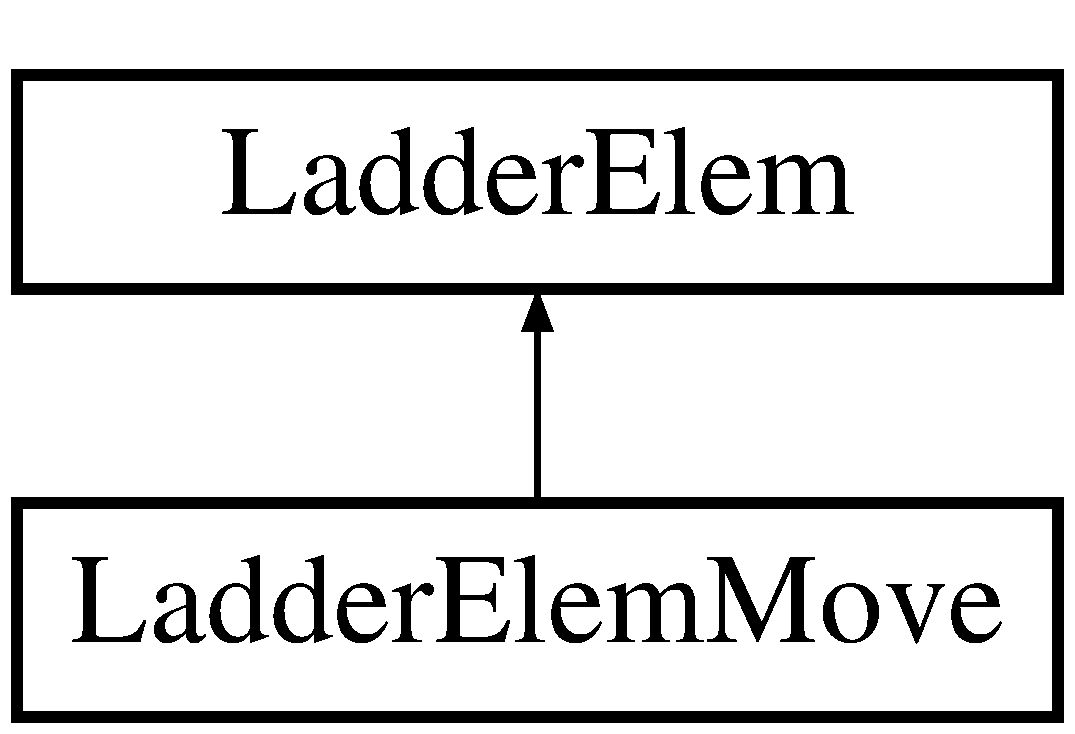
\includegraphics[height=2.000000cm]{class_ladder_elem_move}
\end{center}
\end{figure}
\subsection*{Public Member Functions}
\begin{DoxyCompactItemize}
\item 
\hypertarget{class_ladder_elem_move_a7dae75a067815aedba76c298ea974c1d}{{\bfseries Ladder\-Elem\-Move} (\hyperlink{class_ladder_diagram}{Ladder\-Diagram} $\ast$diagram)}\label{class_ladder_elem_move_a7dae75a067815aedba76c298ea974c1d}

\item 
\hypertarget{class_ladder_elem_move_a266402443b921d0e9efd5ad81a990d89}{pair$<$ string, string $>$ {\bfseries Draw\-T\-X\-T} (void)}\label{class_ladder_elem_move_a266402443b921d0e9efd5ad81a990d89}

\item 
\hypertarget{class_ladder_elem_move_a76ea6383b6fb9f163123badc206225cc}{bool {\bfseries Draw\-G\-U\-I} (bool powered\-Before, void $\ast$data)}\label{class_ladder_elem_move_a76ea6383b6fb9f163123badc206225cc}

\item 
\hypertarget{class_ladder_elem_move_a77b23edfb8ea00b3adeb25d4a6b581ec}{bool {\bfseries Show\-Dialog} (\hyperlink{struct_ladder_context}{Ladder\-Context} context)}\label{class_ladder_elem_move_a77b23edfb8ea00b3adeb25d4a6b581ec}

\item 
\hypertarget{class_ladder_elem_move_acff186c61d99a92e06b19b1a9871cf53}{bool {\bfseries internal\-Generate\-Int\-Code} (\hyperlink{class_int_code}{Int\-Code} \&ic)}\label{class_ladder_elem_move_acff186c61d99a92e06b19b1a9871cf53}

\item 
\hypertarget{class_ladder_elem_move_adad8c2466d0fb36be35ec18e38c1038f}{void $\ast$ {\bfseries get\-Properties} (void)}\label{class_ladder_elem_move_adad8c2466d0fb36be35ec18e38c1038f}

\item 
\hypertarget{class_ladder_elem_move_af9ab2d1a31dad1e607d68dad35d20cb8}{bool {\bfseries Can\-Insert} (\hyperlink{struct_ladder_context}{Ladder\-Context} context)}\label{class_ladder_elem_move_af9ab2d1a31dad1e607d68dad35d20cb8}

\item 
\hypertarget{class_ladder_elem_move_a97a51431de1402768710c053fc6992fb}{void {\bfseries do\-Post\-Insert} (void)}\label{class_ladder_elem_move_a97a51431de1402768710c053fc6992fb}

\item 
\hypertarget{class_ladder_elem_move_a612c88659aa2103b10f6ad981ad3a646}{void {\bfseries do\-Post\-Remove} (void)}\label{class_ladder_elem_move_a612c88659aa2103b10f6ad981ad3a646}

\item 
\hypertarget{class_ladder_elem_move_a77b3b6156e412dd27e36991096e3c428}{int {\bfseries get\-Width\-T\-X\-T} (void)}\label{class_ladder_elem_move_a77b3b6156e412dd27e36991096e3c428}

\item 
\hypertarget{class_ladder_elem_move_ad90f0f9b0f708d6fb55268bd0c5431b9}{\hyperlink{class_ladder_elem}{Ladder\-Elem} $\ast$ {\bfseries Clone} (\hyperlink{class_ladder_diagram}{Ladder\-Diagram} $\ast$diagram)}\label{class_ladder_elem_move_ad90f0f9b0f708d6fb55268bd0c5431b9}

\item 
\hypertarget{class_ladder_elem_move_aeb7d4bf1d57e20d3b4d8467d9ba341e4}{bool {\bfseries accept\-I\-O} (unsigned long id, e\-Type type)}\label{class_ladder_elem_move_aeb7d4bf1d57e20d3b4d8467d9ba341e4}

\item 
\hypertarget{class_ladder_elem_move_aa8c1798a39fe943af835c0d4a891b034}{void {\bfseries update\-I\-O} (\hyperlink{class_ladder_diagram}{Ladder\-Diagram} $\ast$owner, bool is\-Discard)}\label{class_ladder_elem_move_aa8c1798a39fe943af835c0d4a891b034}

\item 
\hypertarget{class_ladder_elem_move_a7c8000cd97a6385c04c21fc63aa35d9c}{e\-Type {\bfseries get\-Allowed\-Type\-I\-O} (unsigned long id)}\label{class_ladder_elem_move_a7c8000cd97a6385c04c21fc63aa35d9c}

\item 
\hypertarget{class_ladder_elem_move_a1b347b9398d495ade4fa92dc77100254}{int {\bfseries Search\-And\-Replace} (unsigned long id\-Search, string s\-New\-Text, bool is\-Replace)}\label{class_ladder_elem_move_a1b347b9398d495ade4fa92dc77100254}

\item 
\hypertarget{class_ladder_elem_move_a73829c673f5ba4efca6491d4ada4409c}{bool {\bfseries internal\-Do\-Undo\-Redo} (bool Is\-Undo, bool is\-Discard, \hyperlink{struct_undo_redo_action}{Undo\-Redo\-Action} \&action)}\label{class_ladder_elem_move_a73829c673f5ba4efca6491d4ada4409c}

\end{DoxyCompactItemize}
\subsection*{Additional Inherited Members}


The documentation for this class was generated from the following files\-:\begin{DoxyCompactItemize}
\item 
F\-:/\-S\-V\-N/\-P\-O\-P\-Tools/Ladder\-Objects.\-h\item 
F\-:/\-S\-V\-N/\-P\-O\-P\-Tools/Ladder\-G\-U\-I.\-cpp\item 
F\-:/\-S\-V\-N/\-P\-O\-P\-Tools/Ladder\-Objects.\-cpp\end{DoxyCompactItemize}

\hypertarget{struct_ladder_elem_move_prop}{\section{Ladder\-Elem\-Move\-Prop Struct Reference}
\label{struct_ladder_elem_move_prop}\index{Ladder\-Elem\-Move\-Prop@{Ladder\-Elem\-Move\-Prop}}
}
\subsection*{Public Attributes}
\begin{DoxyCompactItemize}
\item 
\hypertarget{struct_ladder_elem_move_prop_acda0893434b59d7e40fb5c72c30093f1}{pair$<$ unsigned long, int $>$ {\bfseries id\-Dest}}\label{struct_ladder_elem_move_prop_acda0893434b59d7e40fb5c72c30093f1}

\item 
\hypertarget{struct_ladder_elem_move_prop_aca678dac91f06459e80d146f27836efe}{pair$<$ unsigned long, int $>$ {\bfseries id\-Src}}\label{struct_ladder_elem_move_prop_aca678dac91f06459e80d146f27836efe}

\end{DoxyCompactItemize}


The documentation for this struct was generated from the following file\-:\begin{DoxyCompactItemize}
\item 
F\-:/\-S\-V\-N/\-P\-O\-P\-Tools/Ladder\-Objects.\-h\end{DoxyCompactItemize}

\hypertarget{class_ladder_elem_multiset_d_a}{\section{Ladder\-Elem\-Multiset\-D\-A Class Reference}
\label{class_ladder_elem_multiset_d_a}\index{Ladder\-Elem\-Multiset\-D\-A@{Ladder\-Elem\-Multiset\-D\-A}}
}
Inheritance diagram for Ladder\-Elem\-Multiset\-D\-A\-:\begin{figure}[H]
\begin{center}
\leavevmode
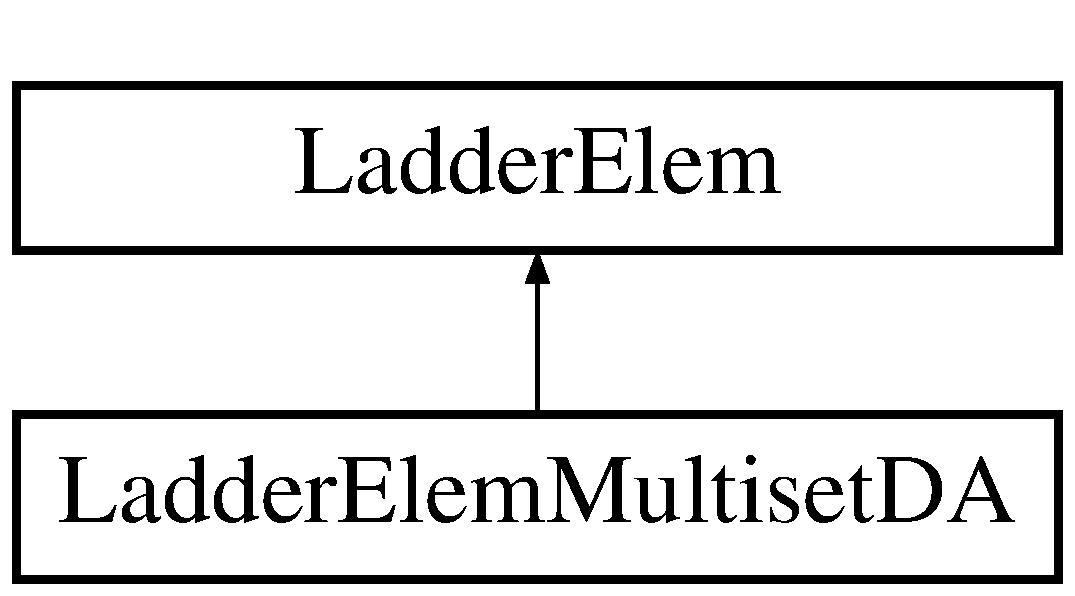
\includegraphics[height=2.000000cm]{class_ladder_elem_multiset_d_a}
\end{center}
\end{figure}
\subsection*{Public Member Functions}
\begin{DoxyCompactItemize}
\item 
\hypertarget{class_ladder_elem_multiset_d_a_ac925e3d61d598cf62aa4d99d702641ef}{{\bfseries Ladder\-Elem\-Multiset\-D\-A} (\hyperlink{class_ladder_diagram}{Ladder\-Diagram} $\ast$diagram)}\label{class_ladder_elem_multiset_d_a_ac925e3d61d598cf62aa4d99d702641ef}

\item 
\hypertarget{class_ladder_elem_multiset_d_a_a6abeeeab83bb90252a3a68db3d8e6afe}{pair$<$ string, string $>$ {\bfseries Draw\-T\-X\-T} (void)}\label{class_ladder_elem_multiset_d_a_a6abeeeab83bb90252a3a68db3d8e6afe}

\item 
\hypertarget{class_ladder_elem_multiset_d_a_a8a93211693b6685f744b06f05695b463}{bool {\bfseries Draw\-G\-U\-I} (bool powered\-Before, void $\ast$data)}\label{class_ladder_elem_multiset_d_a_a8a93211693b6685f744b06f05695b463}

\item 
\hypertarget{class_ladder_elem_multiset_d_a_a61d288dc56482003bff7ffd95d0b7b48}{bool {\bfseries Show\-Dialog} (\hyperlink{struct_ladder_context}{Ladder\-Context} context)}\label{class_ladder_elem_multiset_d_a_a61d288dc56482003bff7ffd95d0b7b48}

\item 
\hypertarget{class_ladder_elem_multiset_d_a_aeb336bd5e33722932aac958c15954f5f}{bool {\bfseries internal\-Generate\-Int\-Code} (\hyperlink{class_int_code}{Int\-Code} \&ic)}\label{class_ladder_elem_multiset_d_a_aeb336bd5e33722932aac958c15954f5f}

\item 
\hypertarget{class_ladder_elem_multiset_d_a_a9d92ef11005ca49e5d51f331efb86f4e}{void $\ast$ {\bfseries get\-Properties} (void)}\label{class_ladder_elem_multiset_d_a_a9d92ef11005ca49e5d51f331efb86f4e}

\item 
\hypertarget{class_ladder_elem_multiset_d_a_aa2da0e9a5caee1ecc222cb4ee860469c}{bool {\bfseries Can\-Insert} (\hyperlink{struct_ladder_context}{Ladder\-Context} context)}\label{class_ladder_elem_multiset_d_a_aa2da0e9a5caee1ecc222cb4ee860469c}

\item 
\hypertarget{class_ladder_elem_multiset_d_a_a9ee7bdb9bb56aa0c6e82f27b7ecad1c2}{void {\bfseries do\-Post\-Insert} (void)}\label{class_ladder_elem_multiset_d_a_a9ee7bdb9bb56aa0c6e82f27b7ecad1c2}

\item 
\hypertarget{class_ladder_elem_multiset_d_a_a6047cd20b91096b7a4b77b7518eebe24}{void {\bfseries do\-Post\-Remove} (void)}\label{class_ladder_elem_multiset_d_a_a6047cd20b91096b7a4b77b7518eebe24}

\item 
\hypertarget{class_ladder_elem_multiset_d_a_aaf61a22c66ba19b45589e91bbd673e5f}{int {\bfseries get\-Width\-T\-X\-T} (void)}\label{class_ladder_elem_multiset_d_a_aaf61a22c66ba19b45589e91bbd673e5f}

\item 
\hypertarget{class_ladder_elem_multiset_d_a_aa84df4f62f991094150a26c6028a3364}{\hyperlink{class_ladder_elem}{Ladder\-Elem} $\ast$ {\bfseries Clone} (\hyperlink{class_ladder_diagram}{Ladder\-Diagram} $\ast$diagram)}\label{class_ladder_elem_multiset_d_a_aa84df4f62f991094150a26c6028a3364}

\item 
\hypertarget{class_ladder_elem_multiset_d_a_ab64fe4bcf33d3d0209f09162756aaa3f}{bool {\bfseries accept\-I\-O} (unsigned long id, e\-Type type)}\label{class_ladder_elem_multiset_d_a_ab64fe4bcf33d3d0209f09162756aaa3f}

\item 
\hypertarget{class_ladder_elem_multiset_d_a_a5fa15bdcd444a729a656d414cf76db1f}{void {\bfseries update\-I\-O} (\hyperlink{class_ladder_diagram}{Ladder\-Diagram} $\ast$owner, bool is\-Discard)}\label{class_ladder_elem_multiset_d_a_a5fa15bdcd444a729a656d414cf76db1f}

\item 
\hypertarget{class_ladder_elem_multiset_d_a_a5b8ca8dbe7b41c400e92bd9d223972d1}{e\-Type {\bfseries get\-Allowed\-Type\-I\-O} (unsigned long id)}\label{class_ladder_elem_multiset_d_a_a5b8ca8dbe7b41c400e92bd9d223972d1}

\item 
\hypertarget{class_ladder_elem_multiset_d_a_a9123844b85e5b4d2d13015cf95ec4f08}{int {\bfseries Search\-And\-Replace} (unsigned long id\-Search, string s\-New\-Text, bool is\-Replace)}\label{class_ladder_elem_multiset_d_a_a9123844b85e5b4d2d13015cf95ec4f08}

\item 
\hypertarget{class_ladder_elem_multiset_d_a_adcb14060745b60e97e56f181e67af4a6}{bool {\bfseries internal\-Do\-Undo\-Redo} (bool Is\-Undo, bool is\-Discard, \hyperlink{struct_undo_redo_action}{Undo\-Redo\-Action} \&action)}\label{class_ladder_elem_multiset_d_a_adcb14060745b60e97e56f181e67af4a6}

\end{DoxyCompactItemize}
\subsection*{Additional Inherited Members}


The documentation for this class was generated from the following files\-:\begin{DoxyCompactItemize}
\item 
F\-:/\-S\-V\-N/\-P\-O\-P\-Tools/Ladder\-Objects.\-h\item 
F\-:/\-S\-V\-N/\-P\-O\-P\-Tools/Ladder\-G\-U\-I.\-cpp\item 
F\-:/\-S\-V\-N/\-P\-O\-P\-Tools/Ladder\-Objects.\-cpp\end{DoxyCompactItemize}

\hypertarget{struct_ladder_elem_multiset_d_a_prop}{\section{Ladder\-Elem\-Multiset\-D\-A\-Prop Struct Reference}
\label{struct_ladder_elem_multiset_d_a_prop}\index{Ladder\-Elem\-Multiset\-D\-A\-Prop@{Ladder\-Elem\-Multiset\-D\-A\-Prop}}
}
\subsection*{Public Attributes}
\begin{DoxyCompactItemize}
\item 
\hypertarget{struct_ladder_elem_multiset_d_a_prop_a309962f7e60acc7fbc639d2c2a04e896}{pair$<$ unsigned long, int $>$ {\bfseries id\-Time}}\label{struct_ladder_elem_multiset_d_a_prop_a309962f7e60acc7fbc639d2c2a04e896}

\item 
\hypertarget{struct_ladder_elem_multiset_d_a_prop_aac19747009febc7bfaf3e7c93a82684f}{pair$<$ unsigned long, int $>$ {\bfseries id\-Desl}}\label{struct_ladder_elem_multiset_d_a_prop_aac19747009febc7bfaf3e7c93a82684f}

\item 
\hypertarget{struct_ladder_elem_multiset_d_a_prop_ad9a577c43fe32f7ab042fdc20cdaa335}{bool {\bfseries linear}}\label{struct_ladder_elem_multiset_d_a_prop_ad9a577c43fe32f7ab042fdc20cdaa335}

\item 
\hypertarget{struct_ladder_elem_multiset_d_a_prop_af383a097741cafe9d60b14c52f7e439e}{bool {\bfseries forward}}\label{struct_ladder_elem_multiset_d_a_prop_af383a097741cafe9d60b14c52f7e439e}

\item 
\hypertarget{struct_ladder_elem_multiset_d_a_prop_af60936faab716772807e0195769fd08d}{bool {\bfseries speedup}}\label{struct_ladder_elem_multiset_d_a_prop_af60936faab716772807e0195769fd08d}

\item 
\hypertarget{struct_ladder_elem_multiset_d_a_prop_ae64be18b062ca774f81cb712c56ef475}{int {\bfseries initval}}\label{struct_ladder_elem_multiset_d_a_prop_ae64be18b062ca774f81cb712c56ef475}

\item 
\hypertarget{struct_ladder_elem_multiset_d_a_prop_ab80ea1e9b54d32c5c1376f9c5eec1cf1}{int {\bfseries type}}\label{struct_ladder_elem_multiset_d_a_prop_ab80ea1e9b54d32c5c1376f9c5eec1cf1}

\item 
\hypertarget{struct_ladder_elem_multiset_d_a_prop_a70923bbc0f669a83e4a033fe0bd82b58}{int {\bfseries gaint}}\label{struct_ladder_elem_multiset_d_a_prop_a70923bbc0f669a83e4a033fe0bd82b58}

\item 
\hypertarget{struct_ladder_elem_multiset_d_a_prop_a0bafd8eb80ca041b78c992c6be4853ed}{int {\bfseries gainr}}\label{struct_ladder_elem_multiset_d_a_prop_a0bafd8eb80ca041b78c992c6be4853ed}

\item 
\hypertarget{struct_ladder_elem_multiset_d_a_prop_a367e9de9b387d8ee7488473981a0dca2}{bool {\bfseries Start\-From\-Current\-Value}}\label{struct_ladder_elem_multiset_d_a_prop_a367e9de9b387d8ee7488473981a0dca2}

\item 
\hypertarget{struct_ladder_elem_multiset_d_a_prop_a5bc493f52de34b08542a5f98a1c08e6d}{int {\bfseries ramp\-\_\-abort\-\_\-mode}}\label{struct_ladder_elem_multiset_d_a_prop_a5bc493f52de34b08542a5f98a1c08e6d}

\end{DoxyCompactItemize}


The documentation for this struct was generated from the following file\-:\begin{DoxyCompactItemize}
\item 
F\-:/\-S\-V\-N/\-P\-O\-P\-Tools/Ladder\-Objects.\-h\end{DoxyCompactItemize}

\hypertarget{class_ladder_elem_one_shot}{\section{Ladder\-Elem\-One\-Shot Class Reference}
\label{class_ladder_elem_one_shot}\index{Ladder\-Elem\-One\-Shot@{Ladder\-Elem\-One\-Shot}}
}
Inheritance diagram for Ladder\-Elem\-One\-Shot\-:\begin{figure}[H]
\begin{center}
\leavevmode
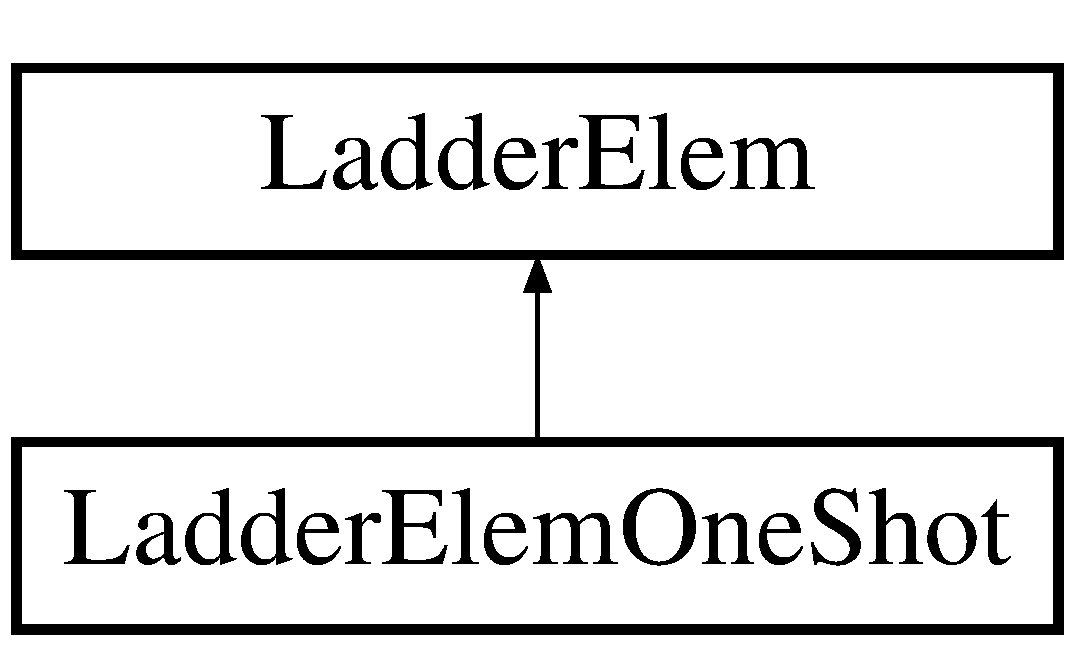
\includegraphics[height=2.000000cm]{class_ladder_elem_one_shot}
\end{center}
\end{figure}
\subsection*{Public Member Functions}
\begin{DoxyCompactItemize}
\item 
\hypertarget{class_ladder_elem_one_shot_a966afd61bc9eefbab5e0d5c3007f5385}{{\bfseries Ladder\-Elem\-One\-Shot} (\hyperlink{class_ladder_diagram}{Ladder\-Diagram} $\ast$diagram, int which)}\label{class_ladder_elem_one_shot_a966afd61bc9eefbab5e0d5c3007f5385}

\item 
\hypertarget{class_ladder_elem_one_shot_a397740a3b18216b746e3b36f01440812}{pair$<$ string, string $>$ {\bfseries Draw\-T\-X\-T} (void)}\label{class_ladder_elem_one_shot_a397740a3b18216b746e3b36f01440812}

\item 
\hypertarget{class_ladder_elem_one_shot_ac20894401f7c2e3a97eaf6ca1e6bcdf3}{bool {\bfseries Draw\-G\-U\-I} (bool powered\-Before, void $\ast$data)}\label{class_ladder_elem_one_shot_ac20894401f7c2e3a97eaf6ca1e6bcdf3}

\item 
\hypertarget{class_ladder_elem_one_shot_a11827bfe25521283b3e2c1131f734e5c}{bool {\bfseries Show\-Dialog} (\hyperlink{struct_ladder_context}{Ladder\-Context} context)}\label{class_ladder_elem_one_shot_a11827bfe25521283b3e2c1131f734e5c}

\item 
\hypertarget{class_ladder_elem_one_shot_a4a3df55397821928d9591905337ae832}{bool {\bfseries internal\-Generate\-Int\-Code} (\hyperlink{class_int_code}{Int\-Code} \&ic)}\label{class_ladder_elem_one_shot_a4a3df55397821928d9591905337ae832}

\item 
\hypertarget{class_ladder_elem_one_shot_a577d55f38ddc6e1039eb5317da139251}{void $\ast$ {\bfseries get\-Properties} (void)}\label{class_ladder_elem_one_shot_a577d55f38ddc6e1039eb5317da139251}

\item 
\hypertarget{class_ladder_elem_one_shot_a0891e800a3c10fd28f7d688cda2de736}{bool {\bfseries Can\-Insert} (\hyperlink{struct_ladder_context}{Ladder\-Context} context)}\label{class_ladder_elem_one_shot_a0891e800a3c10fd28f7d688cda2de736}

\item 
\hypertarget{class_ladder_elem_one_shot_add9906184b5a6123877a450d4a087646}{void {\bfseries do\-Post\-Insert} (void)}\label{class_ladder_elem_one_shot_add9906184b5a6123877a450d4a087646}

\item 
\hypertarget{class_ladder_elem_one_shot_afb336865636017ff96f54b77291ec476}{void {\bfseries do\-Post\-Remove} (void)}\label{class_ladder_elem_one_shot_afb336865636017ff96f54b77291ec476}

\item 
\hypertarget{class_ladder_elem_one_shot_a357ca7bcb5c7b56333ab0eee3e35b2ba}{int {\bfseries get\-Width\-T\-X\-T} (void)}\label{class_ladder_elem_one_shot_a357ca7bcb5c7b56333ab0eee3e35b2ba}

\item 
\hypertarget{class_ladder_elem_one_shot_a0d01c1fb9fe81f819be0c8f680776b71}{\hyperlink{class_ladder_elem}{Ladder\-Elem} $\ast$ {\bfseries Clone} (\hyperlink{class_ladder_diagram}{Ladder\-Diagram} $\ast$diagram)}\label{class_ladder_elem_one_shot_a0d01c1fb9fe81f819be0c8f680776b71}

\item 
\hypertarget{class_ladder_elem_one_shot_aa412f625c3fbb1b5dee09ed8b6249699}{bool {\bfseries accept\-I\-O} (unsigned long id, e\-Type type)}\label{class_ladder_elem_one_shot_aa412f625c3fbb1b5dee09ed8b6249699}

\item 
\hypertarget{class_ladder_elem_one_shot_aae0ad22565a476e65b61b2db3cf861af}{void {\bfseries update\-I\-O} (\hyperlink{class_ladder_diagram}{Ladder\-Diagram} $\ast$owner, bool is\-Discard)}\label{class_ladder_elem_one_shot_aae0ad22565a476e65b61b2db3cf861af}

\item 
\hypertarget{class_ladder_elem_one_shot_a8c5cbda8dbc02b27ab81fbc71bb29e24}{e\-Type {\bfseries get\-Allowed\-Type\-I\-O} (unsigned long id)}\label{class_ladder_elem_one_shot_a8c5cbda8dbc02b27ab81fbc71bb29e24}

\item 
\hypertarget{class_ladder_elem_one_shot_ad79d66343b5a3308a774bd0b0552e77b}{int {\bfseries Search\-And\-Replace} (unsigned long id\-Search, string s\-New\-Text, bool is\-Replace)}\label{class_ladder_elem_one_shot_ad79d66343b5a3308a774bd0b0552e77b}

\item 
\hypertarget{class_ladder_elem_one_shot_a198fdb71c3cf556cca355e64bd910e3b}{bool {\bfseries internal\-Do\-Undo\-Redo} (bool Is\-Undo, bool is\-Discard, \hyperlink{struct_undo_redo_action}{Undo\-Redo\-Action} \&action)}\label{class_ladder_elem_one_shot_a198fdb71c3cf556cca355e64bd910e3b}

\end{DoxyCompactItemize}
\subsection*{Additional Inherited Members}


The documentation for this class was generated from the following files\-:\begin{DoxyCompactItemize}
\item 
F\-:/\-S\-V\-N/\-P\-O\-P\-Tools/Ladder\-Objects.\-h\item 
F\-:/\-S\-V\-N/\-P\-O\-P\-Tools/Ladder\-G\-U\-I.\-cpp\item 
F\-:/\-S\-V\-N/\-P\-O\-P\-Tools/Ladder\-Objects.\-cpp\end{DoxyCompactItemize}

\hypertarget{class_ladder_elem_open_short}{\section{Ladder\-Elem\-Open\-Short Class Reference}
\label{class_ladder_elem_open_short}\index{Ladder\-Elem\-Open\-Short@{Ladder\-Elem\-Open\-Short}}
}
Inheritance diagram for Ladder\-Elem\-Open\-Short\-:\begin{figure}[H]
\begin{center}
\leavevmode
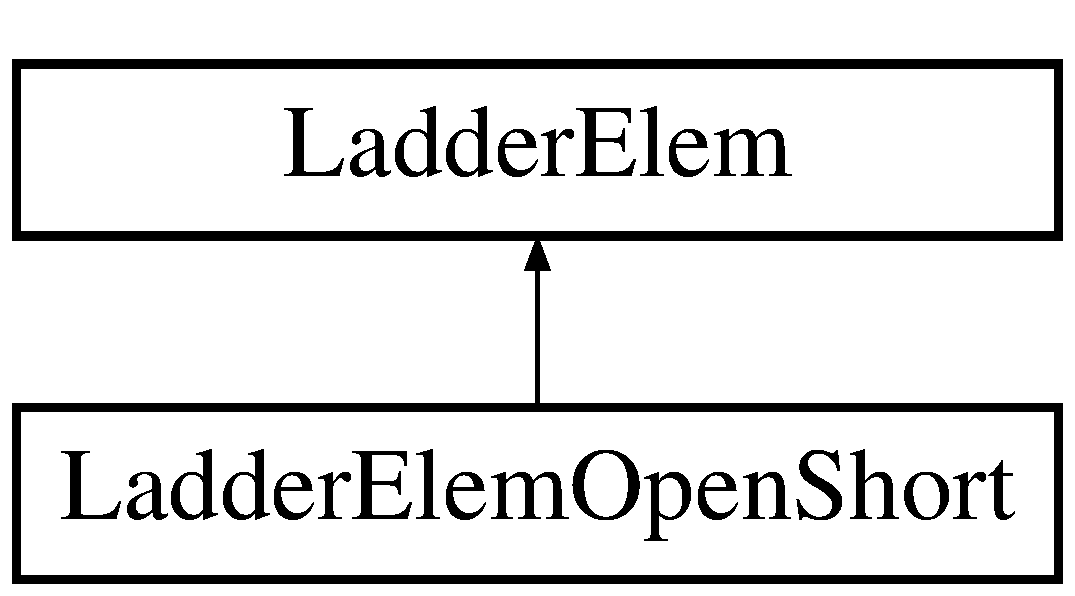
\includegraphics[height=2.000000cm]{class_ladder_elem_open_short}
\end{center}
\end{figure}
\subsection*{Public Member Functions}
\begin{DoxyCompactItemize}
\item 
\hypertarget{class_ladder_elem_open_short_af1822c9fc1834edaff46fc31b5bafa9d}{{\bfseries Ladder\-Elem\-Open\-Short} (\hyperlink{class_ladder_diagram}{Ladder\-Diagram} $\ast$diagram, int which)}\label{class_ladder_elem_open_short_af1822c9fc1834edaff46fc31b5bafa9d}

\item 
\hypertarget{class_ladder_elem_open_short_a00862d473310b4db45e0b49425c68d21}{pair$<$ string, string $>$ {\bfseries Draw\-T\-X\-T} (void)}\label{class_ladder_elem_open_short_a00862d473310b4db45e0b49425c68d21}

\item 
\hypertarget{class_ladder_elem_open_short_a3380096b2435b953fe1005ee560b2240}{bool {\bfseries Draw\-G\-U\-I} (bool powered\-Before, void $\ast$data)}\label{class_ladder_elem_open_short_a3380096b2435b953fe1005ee560b2240}

\item 
\hypertarget{class_ladder_elem_open_short_ad8f2de001973fc4ade29e1d34ab19777}{bool {\bfseries Show\-Dialog} (\hyperlink{struct_ladder_context}{Ladder\-Context} context)}\label{class_ladder_elem_open_short_ad8f2de001973fc4ade29e1d34ab19777}

\item 
\hypertarget{class_ladder_elem_open_short_a80e73eb00806593816293ed513464cc5}{bool {\bfseries internal\-Generate\-Int\-Code} (\hyperlink{class_int_code}{Int\-Code} \&ic)}\label{class_ladder_elem_open_short_a80e73eb00806593816293ed513464cc5}

\item 
\hypertarget{class_ladder_elem_open_short_a9cee8ad1ce9ebcd946d5fc7051967318}{void $\ast$ {\bfseries get\-Properties} (void)}\label{class_ladder_elem_open_short_a9cee8ad1ce9ebcd946d5fc7051967318}

\item 
\hypertarget{class_ladder_elem_open_short_aa3e46c028eb95f18cf845cb565ea0798}{bool {\bfseries Can\-Insert} (\hyperlink{struct_ladder_context}{Ladder\-Context} context)}\label{class_ladder_elem_open_short_aa3e46c028eb95f18cf845cb565ea0798}

\item 
\hypertarget{class_ladder_elem_open_short_a59e4c2ea5272f85aef3f44c1b354f31e}{void {\bfseries do\-Post\-Insert} (void)}\label{class_ladder_elem_open_short_a59e4c2ea5272f85aef3f44c1b354f31e}

\item 
\hypertarget{class_ladder_elem_open_short_a3d935834a2ff63b9b5eaf89d4d0ad107}{void {\bfseries do\-Post\-Remove} (void)}\label{class_ladder_elem_open_short_a3d935834a2ff63b9b5eaf89d4d0ad107}

\item 
\hypertarget{class_ladder_elem_open_short_ae8cb40618e6bc686fbbc9e3ea508527a}{int {\bfseries get\-Width\-T\-X\-T} (void)}\label{class_ladder_elem_open_short_ae8cb40618e6bc686fbbc9e3ea508527a}

\item 
\hypertarget{class_ladder_elem_open_short_afbecb7420ee42b327880be0ee62c6509}{\hyperlink{class_ladder_elem}{Ladder\-Elem} $\ast$ {\bfseries Clone} (\hyperlink{class_ladder_diagram}{Ladder\-Diagram} $\ast$diagram)}\label{class_ladder_elem_open_short_afbecb7420ee42b327880be0ee62c6509}

\item 
\hypertarget{class_ladder_elem_open_short_a50df78f133a0f00dae017273b70fdd90}{bool {\bfseries accept\-I\-O} (unsigned long id, e\-Type type)}\label{class_ladder_elem_open_short_a50df78f133a0f00dae017273b70fdd90}

\item 
\hypertarget{class_ladder_elem_open_short_aa01844fa4acd78042c70d4e52114195c}{void {\bfseries update\-I\-O} (\hyperlink{class_ladder_diagram}{Ladder\-Diagram} $\ast$owner, bool is\-Discard)}\label{class_ladder_elem_open_short_aa01844fa4acd78042c70d4e52114195c}

\item 
\hypertarget{class_ladder_elem_open_short_ab9b47d8deadfa8e212ea24536cc3dd60}{e\-Type {\bfseries get\-Allowed\-Type\-I\-O} (unsigned long id)}\label{class_ladder_elem_open_short_ab9b47d8deadfa8e212ea24536cc3dd60}

\item 
\hypertarget{class_ladder_elem_open_short_a0e9b3854d44afefd0117e204659bda60}{int {\bfseries Search\-And\-Replace} (unsigned long id\-Search, string s\-New\-Text, bool is\-Replace)}\label{class_ladder_elem_open_short_a0e9b3854d44afefd0117e204659bda60}

\item 
\hypertarget{class_ladder_elem_open_short_ab6d22c4a0deb03b5a3bfb9c54ec2dcb8}{bool {\bfseries internal\-Do\-Undo\-Redo} (bool Is\-Undo, bool is\-Discard, \hyperlink{struct_undo_redo_action}{Undo\-Redo\-Action} \&action)}\label{class_ladder_elem_open_short_ab6d22c4a0deb03b5a3bfb9c54ec2dcb8}

\end{DoxyCompactItemize}
\subsection*{Additional Inherited Members}


The documentation for this class was generated from the following files\-:\begin{DoxyCompactItemize}
\item 
F\-:/\-S\-V\-N/\-P\-O\-P\-Tools/Ladder\-Objects.\-h\item 
F\-:/\-S\-V\-N/\-P\-O\-P\-Tools/Ladder\-G\-U\-I.\-cpp\item 
F\-:/\-S\-V\-N/\-P\-O\-P\-Tools/Ladder\-Objects.\-cpp\end{DoxyCompactItemize}

\hypertarget{class_ladder_elem_persist}{\section{Ladder\-Elem\-Persist Class Reference}
\label{class_ladder_elem_persist}\index{Ladder\-Elem\-Persist@{Ladder\-Elem\-Persist}}
}
Inheritance diagram for Ladder\-Elem\-Persist\-:\begin{figure}[H]
\begin{center}
\leavevmode
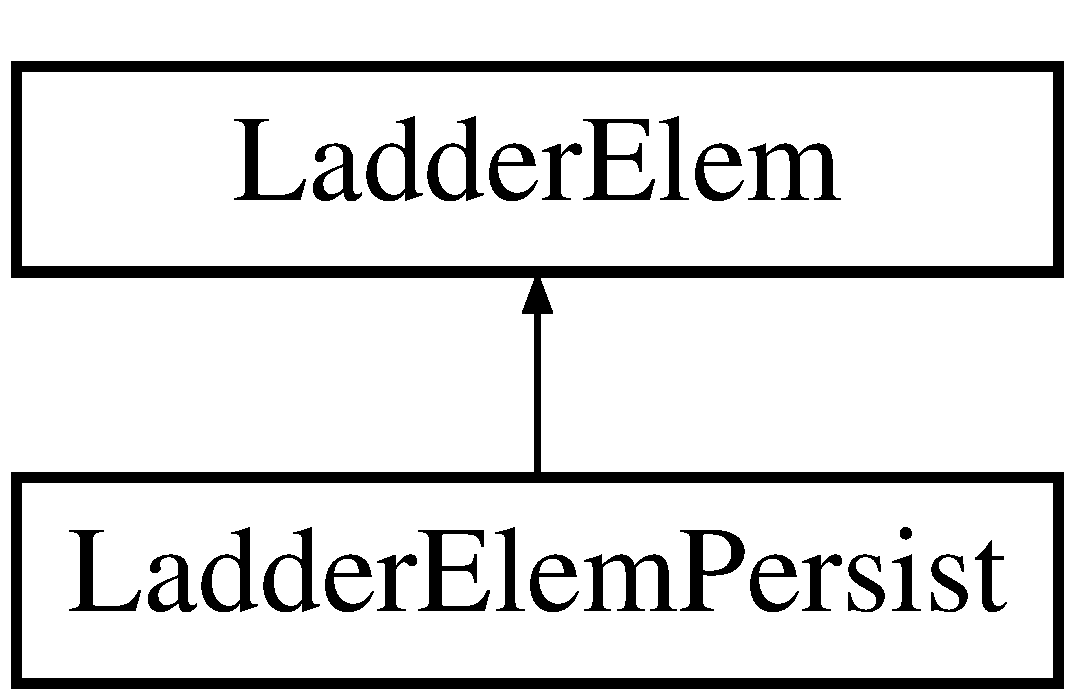
\includegraphics[height=2.000000cm]{class_ladder_elem_persist}
\end{center}
\end{figure}
\subsection*{Public Member Functions}
\begin{DoxyCompactItemize}
\item 
\hypertarget{class_ladder_elem_persist_a497136effcfffa1f9871e6661ee7aff6}{{\bfseries Ladder\-Elem\-Persist} (\hyperlink{class_ladder_diagram}{Ladder\-Diagram} $\ast$diagram)}\label{class_ladder_elem_persist_a497136effcfffa1f9871e6661ee7aff6}

\item 
\hypertarget{class_ladder_elem_persist_a7a91ae65a2459792eadcaab7c7e3e9b7}{pair$<$ string, string $>$ {\bfseries Draw\-T\-X\-T} (void)}\label{class_ladder_elem_persist_a7a91ae65a2459792eadcaab7c7e3e9b7}

\item 
\hypertarget{class_ladder_elem_persist_ac33ec799ca70807b6d0628803d42da8b}{bool {\bfseries Draw\-G\-U\-I} (bool powered\-Before, void $\ast$data)}\label{class_ladder_elem_persist_ac33ec799ca70807b6d0628803d42da8b}

\item 
\hypertarget{class_ladder_elem_persist_ad493c8ed0deec93e523149b8be32cd51}{bool {\bfseries Show\-Dialog} (\hyperlink{struct_ladder_context}{Ladder\-Context} context)}\label{class_ladder_elem_persist_ad493c8ed0deec93e523149b8be32cd51}

\item 
\hypertarget{class_ladder_elem_persist_a78b662e1699270fa77744e3d7137667b}{bool {\bfseries internal\-Generate\-Int\-Code} (\hyperlink{class_int_code}{Int\-Code} \&ic)}\label{class_ladder_elem_persist_a78b662e1699270fa77744e3d7137667b}

\item 
\hypertarget{class_ladder_elem_persist_a588040dbbcea827f4a4252ab32e27a13}{void $\ast$ {\bfseries get\-Properties} (void)}\label{class_ladder_elem_persist_a588040dbbcea827f4a4252ab32e27a13}

\item 
\hypertarget{class_ladder_elem_persist_a71871772ac873e13241d0185eeb9decb}{bool {\bfseries Can\-Insert} (\hyperlink{struct_ladder_context}{Ladder\-Context} context)}\label{class_ladder_elem_persist_a71871772ac873e13241d0185eeb9decb}

\item 
\hypertarget{class_ladder_elem_persist_a375bca73d5cd908028480b9abebbcf91}{void {\bfseries do\-Post\-Insert} (void)}\label{class_ladder_elem_persist_a375bca73d5cd908028480b9abebbcf91}

\item 
\hypertarget{class_ladder_elem_persist_aefd8f02d6273b3be3783f424622db2e0}{void {\bfseries do\-Post\-Remove} (void)}\label{class_ladder_elem_persist_aefd8f02d6273b3be3783f424622db2e0}

\item 
\hypertarget{class_ladder_elem_persist_a563dd31c5be7006c6dc0cab97c7b0996}{int {\bfseries get\-Width\-T\-X\-T} (void)}\label{class_ladder_elem_persist_a563dd31c5be7006c6dc0cab97c7b0996}

\item 
\hypertarget{class_ladder_elem_persist_abfccb1b08aca106f6650a10838431fee}{\hyperlink{class_ladder_elem}{Ladder\-Elem} $\ast$ {\bfseries Clone} (\hyperlink{class_ladder_diagram}{Ladder\-Diagram} $\ast$diagram)}\label{class_ladder_elem_persist_abfccb1b08aca106f6650a10838431fee}

\item 
\hypertarget{class_ladder_elem_persist_a827d7cee126a500d5affb877d9344f67}{bool {\bfseries accept\-I\-O} (unsigned long id, e\-Type type)}\label{class_ladder_elem_persist_a827d7cee126a500d5affb877d9344f67}

\item 
\hypertarget{class_ladder_elem_persist_aa0609b95ddc6e12532816dcab0717dcb}{void {\bfseries update\-I\-O} (\hyperlink{class_ladder_diagram}{Ladder\-Diagram} $\ast$owner, bool is\-Discard)}\label{class_ladder_elem_persist_aa0609b95ddc6e12532816dcab0717dcb}

\item 
\hypertarget{class_ladder_elem_persist_af2d7070875ce04ac9799f7600949efe9}{e\-Type {\bfseries get\-Allowed\-Type\-I\-O} (unsigned long id)}\label{class_ladder_elem_persist_af2d7070875ce04ac9799f7600949efe9}

\item 
\hypertarget{class_ladder_elem_persist_a9a63ab7f2627c6fce768672ee5db8657}{int {\bfseries Search\-And\-Replace} (unsigned long id\-Search, string s\-New\-Text, bool is\-Replace)}\label{class_ladder_elem_persist_a9a63ab7f2627c6fce768672ee5db8657}

\item 
\hypertarget{class_ladder_elem_persist_a7d86bc2bbf6fa2b40b5ed2fbafb01146}{bool {\bfseries internal\-Do\-Undo\-Redo} (bool Is\-Undo, bool is\-Discard, \hyperlink{struct_undo_redo_action}{Undo\-Redo\-Action} \&action)}\label{class_ladder_elem_persist_a7d86bc2bbf6fa2b40b5ed2fbafb01146}

\end{DoxyCompactItemize}
\subsection*{Additional Inherited Members}


The documentation for this class was generated from the following files\-:\begin{DoxyCompactItemize}
\item 
F\-:/\-S\-V\-N/\-P\-O\-P\-Tools/Ladder\-Objects.\-h\item 
F\-:/\-S\-V\-N/\-P\-O\-P\-Tools/Ladder\-G\-U\-I.\-cpp\item 
F\-:/\-S\-V\-N/\-P\-O\-P\-Tools/Ladder\-Objects.\-cpp\end{DoxyCompactItemize}

\hypertarget{struct_ladder_elem_persist_prop}{\section{Ladder\-Elem\-Persist\-Prop Struct Reference}
\label{struct_ladder_elem_persist_prop}\index{Ladder\-Elem\-Persist\-Prop@{Ladder\-Elem\-Persist\-Prop}}
}
\subsection*{Public Attributes}
\begin{DoxyCompactItemize}
\item 
\hypertarget{struct_ladder_elem_persist_prop_a1deaef25ec896ec2e649842de61c8058}{pair$<$ unsigned long, int $>$ {\bfseries id\-Var}}\label{struct_ladder_elem_persist_prop_a1deaef25ec896ec2e649842de61c8058}

\end{DoxyCompactItemize}


The documentation for this struct was generated from the following file\-:\begin{DoxyCompactItemize}
\item 
F\-:/\-S\-V\-N/\-P\-O\-P\-Tools/Ladder\-Objects.\-h\end{DoxyCompactItemize}

\hypertarget{class_ladder_elem_p_i_d}{\section{Ladder\-Elem\-P\-I\-D Class Reference}
\label{class_ladder_elem_p_i_d}\index{Ladder\-Elem\-P\-I\-D@{Ladder\-Elem\-P\-I\-D}}
}
Inheritance diagram for Ladder\-Elem\-P\-I\-D\-:\begin{figure}[H]
\begin{center}
\leavevmode
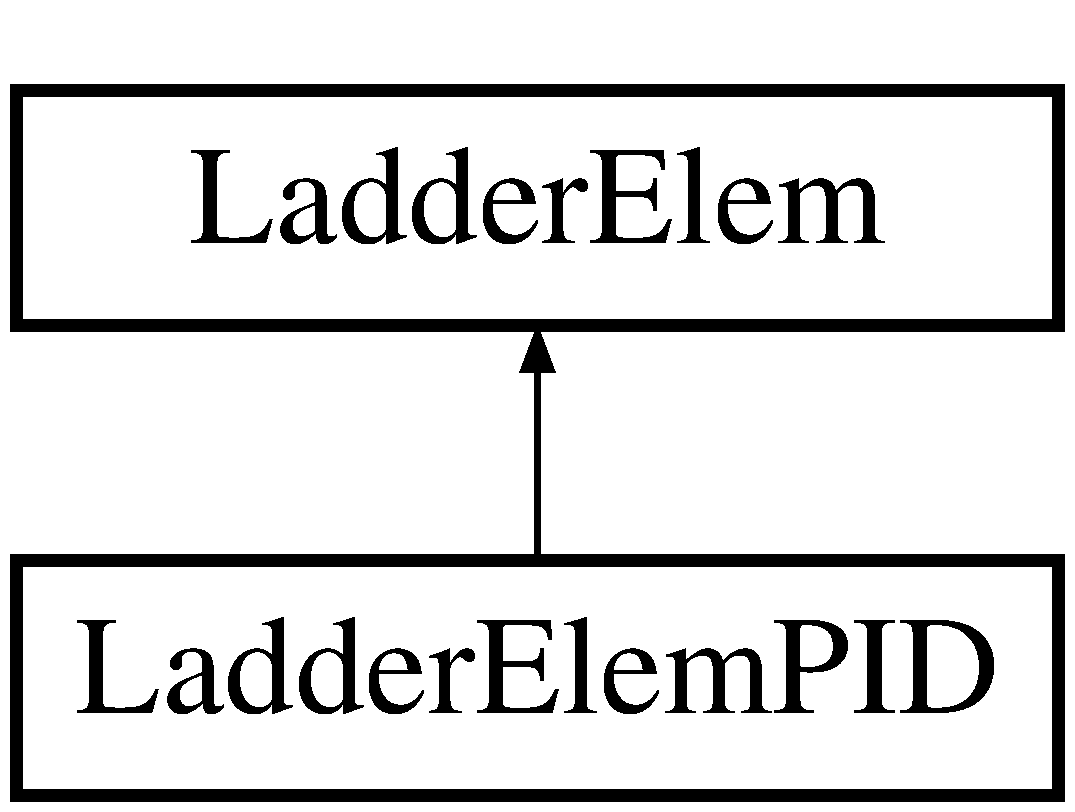
\includegraphics[height=2.000000cm]{class_ladder_elem_p_i_d}
\end{center}
\end{figure}
\subsection*{Public Member Functions}
\begin{DoxyCompactItemize}
\item 
\hypertarget{class_ladder_elem_p_i_d_ab0627f755af374ed7790e3a462841ae2}{{\bfseries Ladder\-Elem\-P\-I\-D} (\hyperlink{class_ladder_diagram}{Ladder\-Diagram} $\ast$diagram)}\label{class_ladder_elem_p_i_d_ab0627f755af374ed7790e3a462841ae2}

\item 
\hypertarget{class_ladder_elem_p_i_d_a1c29d13b8bbe0c238bd05c2b73d9b115}{pair$<$ string, string $>$ {\bfseries Draw\-T\-X\-T} (void)}\label{class_ladder_elem_p_i_d_a1c29d13b8bbe0c238bd05c2b73d9b115}

\item 
\hypertarget{class_ladder_elem_p_i_d_acff9faa46649e9da7125bbcaa0a20b5b}{bool {\bfseries Draw\-G\-U\-I} (bool powered\-Before, void $\ast$data)}\label{class_ladder_elem_p_i_d_acff9faa46649e9da7125bbcaa0a20b5b}

\item 
\hypertarget{class_ladder_elem_p_i_d_aa916b68a41de267712e585b3322bf138}{bool {\bfseries Show\-Dialog} (\hyperlink{struct_ladder_context}{Ladder\-Context} context)}\label{class_ladder_elem_p_i_d_aa916b68a41de267712e585b3322bf138}

\item 
\hypertarget{class_ladder_elem_p_i_d_a1900417813a2ac6d933a0b52fb6db2ff}{bool {\bfseries internal\-Generate\-Int\-Code} (\hyperlink{class_int_code}{Int\-Code} \&ic)}\label{class_ladder_elem_p_i_d_a1900417813a2ac6d933a0b52fb6db2ff}

\item 
\hypertarget{class_ladder_elem_p_i_d_a7788f713b61b0d0abc954faa23ae8d0c}{void $\ast$ {\bfseries get\-Properties} (void)}\label{class_ladder_elem_p_i_d_a7788f713b61b0d0abc954faa23ae8d0c}

\item 
\hypertarget{class_ladder_elem_p_i_d_a4e38abba01987edfddba35a4da192ff9}{bool {\bfseries Can\-Insert} (\hyperlink{struct_ladder_context}{Ladder\-Context} context)}\label{class_ladder_elem_p_i_d_a4e38abba01987edfddba35a4da192ff9}

\item 
\hypertarget{class_ladder_elem_p_i_d_a260608ceb315058522655c457362dbda}{void {\bfseries do\-Post\-Insert} (void)}\label{class_ladder_elem_p_i_d_a260608ceb315058522655c457362dbda}

\item 
\hypertarget{class_ladder_elem_p_i_d_a13ba267bc87b5c9056997ed92c756d8e}{void {\bfseries do\-Post\-Remove} (void)}\label{class_ladder_elem_p_i_d_a13ba267bc87b5c9056997ed92c756d8e}

\item 
\hypertarget{class_ladder_elem_p_i_d_a48cc1656c309ed79f7d0bf195d2d5aba}{int {\bfseries get\-Width\-T\-X\-T} (void)}\label{class_ladder_elem_p_i_d_a48cc1656c309ed79f7d0bf195d2d5aba}

\item 
\hypertarget{class_ladder_elem_p_i_d_a5d1ed993dab797402e5dc612f151cf90}{\hyperlink{class_ladder_elem}{Ladder\-Elem} $\ast$ {\bfseries Clone} (\hyperlink{class_ladder_diagram}{Ladder\-Diagram} $\ast$diagram)}\label{class_ladder_elem_p_i_d_a5d1ed993dab797402e5dc612f151cf90}

\item 
\hypertarget{class_ladder_elem_p_i_d_aba66ff4d3879839feab5d9702d856e70}{bool {\bfseries accept\-I\-O} (unsigned long id, e\-Type type)}\label{class_ladder_elem_p_i_d_aba66ff4d3879839feab5d9702d856e70}

\item 
\hypertarget{class_ladder_elem_p_i_d_a4577ebcf62fa5175687c49c1b3155792}{void {\bfseries update\-I\-O} (\hyperlink{class_ladder_diagram}{Ladder\-Diagram} $\ast$owner, bool is\-Discard)}\label{class_ladder_elem_p_i_d_a4577ebcf62fa5175687c49c1b3155792}

\item 
\hypertarget{class_ladder_elem_p_i_d_a31f93487376d081f882086c14d396946}{e\-Type {\bfseries get\-Allowed\-Type\-I\-O} (unsigned long id)}\label{class_ladder_elem_p_i_d_a31f93487376d081f882086c14d396946}

\item 
\hypertarget{class_ladder_elem_p_i_d_a24bca9c3941397d8488edafac3f03247}{int {\bfseries Search\-And\-Replace} (unsigned long id\-Search, string s\-New\-Text, bool is\-Replace)}\label{class_ladder_elem_p_i_d_a24bca9c3941397d8488edafac3f03247}

\item 
\hypertarget{class_ladder_elem_p_i_d_af6af6aeaa66b6051d70c3a3b81fd44d8}{bool {\bfseries internal\-Do\-Undo\-Redo} (bool Is\-Undo, bool is\-Discard, \hyperlink{struct_undo_redo_action}{Undo\-Redo\-Action} \&action)}\label{class_ladder_elem_p_i_d_af6af6aeaa66b6051d70c3a3b81fd44d8}

\end{DoxyCompactItemize}
\subsection*{Additional Inherited Members}


The documentation for this class was generated from the following files\-:\begin{DoxyCompactItemize}
\item 
F\-:/\-S\-V\-N/\-P\-O\-P\-Tools/Ladder\-Objects.\-h\item 
F\-:/\-S\-V\-N/\-P\-O\-P\-Tools/Ladder\-G\-U\-I.\-cpp\item 
F\-:/\-S\-V\-N/\-P\-O\-P\-Tools/Ladder\-Objects.\-cpp\end{DoxyCompactItemize}

\hypertarget{struct_ladder_elem_p_i_d_prop}{\section{Ladder\-Elem\-P\-I\-D\-Prop Struct Reference}
\label{struct_ladder_elem_p_i_d_prop}\index{Ladder\-Elem\-P\-I\-D\-Prop@{Ladder\-Elem\-P\-I\-D\-Prop}}
}
\subsection*{Public Attributes}
\begin{DoxyCompactItemize}
\item 
\hypertarget{struct_ladder_elem_p_i_d_prop_a960ce48c1f836807b9f0b56f8fd48921}{pair$<$ unsigned long, int $>$ {\bfseries id\-Setpoint}}\label{struct_ladder_elem_p_i_d_prop_a960ce48c1f836807b9f0b56f8fd48921}

\item 
\hypertarget{struct_ladder_elem_p_i_d_prop_a92dfc0233414054d9a4487bf35f3fbc0}{pair$<$ unsigned long, int $>$ {\bfseries id\-Process\-Value}}\label{struct_ladder_elem_p_i_d_prop_a92dfc0233414054d9a4487bf35f3fbc0}

\item 
\hypertarget{struct_ladder_elem_p_i_d_prop_a1dcf0a93e53852b5920dcf850a32e07d}{pair$<$ unsigned long, int $>$ {\bfseries id\-Output}}\label{struct_ladder_elem_p_i_d_prop_a1dcf0a93e53852b5920dcf850a32e07d}

\item 
\hypertarget{struct_ladder_elem_p_i_d_prop_a72641b6383c961f31f3e3d581e0dff52}{pair$<$ unsigned long, int $>$ {\bfseries id\-Gain\-P}}\label{struct_ladder_elem_p_i_d_prop_a72641b6383c961f31f3e3d581e0dff52}

\item 
\hypertarget{struct_ladder_elem_p_i_d_prop_ad198dc63b90cd599d1fa8f3804cb068d}{pair$<$ unsigned long, int $>$ {\bfseries id\-Gain\-I}}\label{struct_ladder_elem_p_i_d_prop_ad198dc63b90cd599d1fa8f3804cb068d}

\item 
\hypertarget{struct_ladder_elem_p_i_d_prop_aeb6911d0331a2f6bd898308934ea9dc4}{pair$<$ unsigned long, int $>$ {\bfseries id\-Gain\-D}}\label{struct_ladder_elem_p_i_d_prop_aeb6911d0331a2f6bd898308934ea9dc4}

\end{DoxyCompactItemize}


The documentation for this struct was generated from the following file\-:\begin{DoxyCompactItemize}
\item 
F\-:/\-S\-V\-N/\-P\-O\-P\-Tools/Ladder\-Objects.\-h\end{DoxyCompactItemize}

\hypertarget{class_ladder_elem_piecewise}{\section{Ladder\-Elem\-Piecewise Class Reference}
\label{class_ladder_elem_piecewise}\index{Ladder\-Elem\-Piecewise@{Ladder\-Elem\-Piecewise}}
}
Inheritance diagram for Ladder\-Elem\-Piecewise\-:\begin{figure}[H]
\begin{center}
\leavevmode
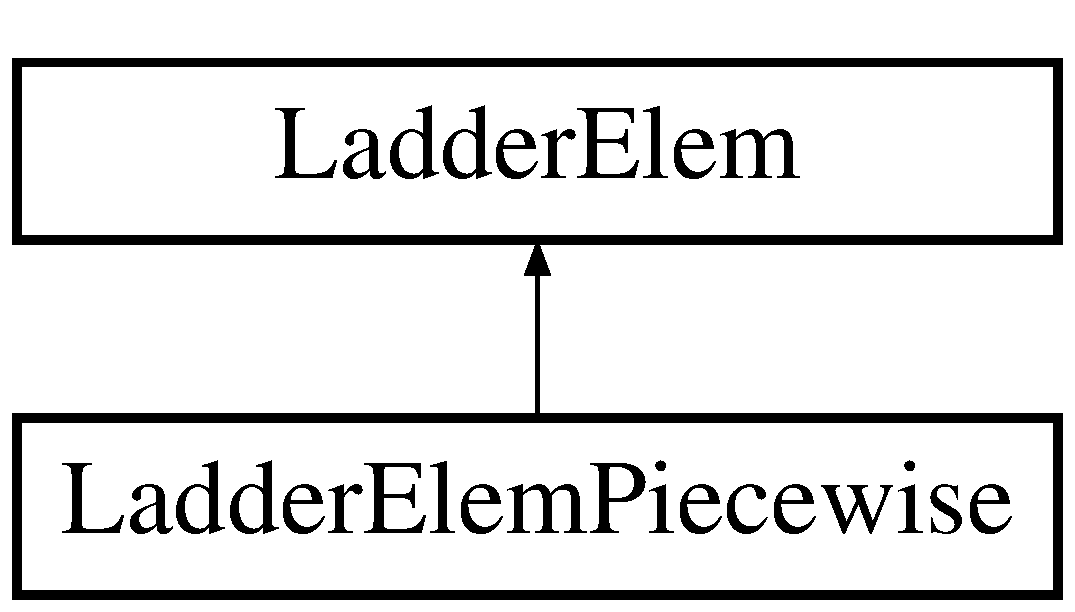
\includegraphics[height=2.000000cm]{class_ladder_elem_piecewise}
\end{center}
\end{figure}
\subsection*{Public Member Functions}
\begin{DoxyCompactItemize}
\item 
\hypertarget{class_ladder_elem_piecewise_adb8df9272f68d87cff9e4dd66d92876a}{{\bfseries Ladder\-Elem\-Piecewise} (\hyperlink{class_ladder_diagram}{Ladder\-Diagram} $\ast$diagram)}\label{class_ladder_elem_piecewise_adb8df9272f68d87cff9e4dd66d92876a}

\item 
\hypertarget{class_ladder_elem_piecewise_a0a59dab2a9e9a07ed8a270f00d094d16}{pair$<$ string, string $>$ {\bfseries Draw\-T\-X\-T} (void)}\label{class_ladder_elem_piecewise_a0a59dab2a9e9a07ed8a270f00d094d16}

\item 
\hypertarget{class_ladder_elem_piecewise_a1aa86c24987519214dffd262f93bdeb9}{bool {\bfseries Draw\-G\-U\-I} (bool powered\-Before, void $\ast$data)}\label{class_ladder_elem_piecewise_a1aa86c24987519214dffd262f93bdeb9}

\item 
\hypertarget{class_ladder_elem_piecewise_aeeaa636b04e697e4bd47c5477200a340}{bool {\bfseries Show\-Dialog} (\hyperlink{struct_ladder_context}{Ladder\-Context} context)}\label{class_ladder_elem_piecewise_aeeaa636b04e697e4bd47c5477200a340}

\item 
\hypertarget{class_ladder_elem_piecewise_a593aa5dab9696076795e2c13b8c6acfb}{bool {\bfseries internal\-Generate\-Int\-Code} (\hyperlink{class_int_code}{Int\-Code} \&ic)}\label{class_ladder_elem_piecewise_a593aa5dab9696076795e2c13b8c6acfb}

\item 
\hypertarget{class_ladder_elem_piecewise_a91d725552a5aa385061d97bc6c53bfc4}{void $\ast$ {\bfseries get\-Properties} (void)}\label{class_ladder_elem_piecewise_a91d725552a5aa385061d97bc6c53bfc4}

\item 
\hypertarget{class_ladder_elem_piecewise_a8325f55e3f847759396f5e1e89dbe39d}{bool {\bfseries Can\-Insert} (\hyperlink{struct_ladder_context}{Ladder\-Context} context)}\label{class_ladder_elem_piecewise_a8325f55e3f847759396f5e1e89dbe39d}

\item 
\hypertarget{class_ladder_elem_piecewise_a4d6c9eb4d20f0cc8d943370190b271e5}{void {\bfseries do\-Post\-Insert} (void)}\label{class_ladder_elem_piecewise_a4d6c9eb4d20f0cc8d943370190b271e5}

\item 
\hypertarget{class_ladder_elem_piecewise_ad3e67e9e402465f9c34ee03e3653e692}{void {\bfseries do\-Post\-Remove} (void)}\label{class_ladder_elem_piecewise_ad3e67e9e402465f9c34ee03e3653e692}

\item 
\hypertarget{class_ladder_elem_piecewise_a8f49da1dbcd986200bf43e4884cdff75}{int {\bfseries get\-Width\-T\-X\-T} (void)}\label{class_ladder_elem_piecewise_a8f49da1dbcd986200bf43e4884cdff75}

\item 
\hypertarget{class_ladder_elem_piecewise_a17d9c8d2c5ae67e96d076e8dc36b39dc}{\hyperlink{class_ladder_elem}{Ladder\-Elem} $\ast$ {\bfseries Clone} (\hyperlink{class_ladder_diagram}{Ladder\-Diagram} $\ast$diagram)}\label{class_ladder_elem_piecewise_a17d9c8d2c5ae67e96d076e8dc36b39dc}

\item 
\hypertarget{class_ladder_elem_piecewise_ad55fc2dd1cc43c1961038f0ee0138c7d}{bool {\bfseries accept\-I\-O} (unsigned long id, e\-Type type)}\label{class_ladder_elem_piecewise_ad55fc2dd1cc43c1961038f0ee0138c7d}

\item 
\hypertarget{class_ladder_elem_piecewise_a1e539a0fd8bac0520162c328e33eda04}{void {\bfseries update\-I\-O} (\hyperlink{class_ladder_diagram}{Ladder\-Diagram} $\ast$owner, bool is\-Discard)}\label{class_ladder_elem_piecewise_a1e539a0fd8bac0520162c328e33eda04}

\item 
\hypertarget{class_ladder_elem_piecewise_a852014c9fb3bd225ca1bcb6e1ca99ebf}{e\-Type {\bfseries get\-Allowed\-Type\-I\-O} (unsigned long id)}\label{class_ladder_elem_piecewise_a852014c9fb3bd225ca1bcb6e1ca99ebf}

\item 
\hypertarget{class_ladder_elem_piecewise_aeb54b853ec3cb685e02e3cef715d1d27}{int {\bfseries Search\-And\-Replace} (unsigned long id\-Search, string s\-New\-Text, bool is\-Replace)}\label{class_ladder_elem_piecewise_aeb54b853ec3cb685e02e3cef715d1d27}

\item 
\hypertarget{class_ladder_elem_piecewise_a0d05f944527e1a3d9dd08a15a9643996}{bool {\bfseries internal\-Do\-Undo\-Redo} (bool Is\-Undo, bool is\-Discard, \hyperlink{struct_undo_redo_action}{Undo\-Redo\-Action} \&action)}\label{class_ladder_elem_piecewise_a0d05f944527e1a3d9dd08a15a9643996}

\end{DoxyCompactItemize}
\subsection*{Additional Inherited Members}


The documentation for this class was generated from the following files\-:\begin{DoxyCompactItemize}
\item 
F\-:/\-S\-V\-N/\-P\-O\-P\-Tools/Ladder\-Objects.\-h\item 
F\-:/\-S\-V\-N/\-P\-O\-P\-Tools/Ladder\-G\-U\-I.\-cpp\item 
F\-:/\-S\-V\-N/\-P\-O\-P\-Tools/Ladder\-Objects.\-cpp\end{DoxyCompactItemize}

\hypertarget{struct_ladder_elem_piecewise_prop}{\section{Ladder\-Elem\-Piecewise\-Prop Struct Reference}
\label{struct_ladder_elem_piecewise_prop}\index{Ladder\-Elem\-Piecewise\-Prop@{Ladder\-Elem\-Piecewise\-Prop}}
}
\subsection*{Public Attributes}
\begin{DoxyCompactItemize}
\item 
\hypertarget{struct_ladder_elem_piecewise_prop_aaf8f704fac83cda77b832566cd077b07}{pair$<$ unsigned long, int $>$ {\bfseries id\-Dest}}\label{struct_ladder_elem_piecewise_prop_aaf8f704fac83cda77b832566cd077b07}

\item 
\hypertarget{struct_ladder_elem_piecewise_prop_a801ed3129b011fd115a77b99efc905e3}{pair$<$ unsigned long, int $>$ {\bfseries id\-Index}}\label{struct_ladder_elem_piecewise_prop_a801ed3129b011fd115a77b99efc905e3}

\item 
\hypertarget{struct_ladder_elem_piecewise_prop_a26a10bcedafa2ea5c56177d6fa15c6e3}{int {\bfseries count}}\label{struct_ladder_elem_piecewise_prop_a26a10bcedafa2ea5c56177d6fa15c6e3}

\item 
\hypertarget{struct_ladder_elem_piecewise_prop_ad693dbe808f39e3db8c621115e9bf7bd}{array$<$ long, \\*
M\-A\-X\-\_\-\-L\-O\-O\-K\-\_\-\-U\-P\-\_\-\-T\-A\-B\-L\-E\-\_\-\-L\-E\-N $>$ {\bfseries vals}}\label{struct_ladder_elem_piecewise_prop_ad693dbe808f39e3db8c621115e9bf7bd}

\end{DoxyCompactItemize}


The documentation for this struct was generated from the following file\-:\begin{DoxyCompactItemize}
\item 
F\-:/\-S\-V\-N/\-P\-O\-P\-Tools/Ladder\-Objects.\-h\end{DoxyCompactItemize}

\hypertarget{class_ladder_elem_place_holder}{\section{Ladder\-Elem\-Place\-Holder Class Reference}
\label{class_ladder_elem_place_holder}\index{Ladder\-Elem\-Place\-Holder@{Ladder\-Elem\-Place\-Holder}}
}
Inheritance diagram for Ladder\-Elem\-Place\-Holder\-:\begin{figure}[H]
\begin{center}
\leavevmode
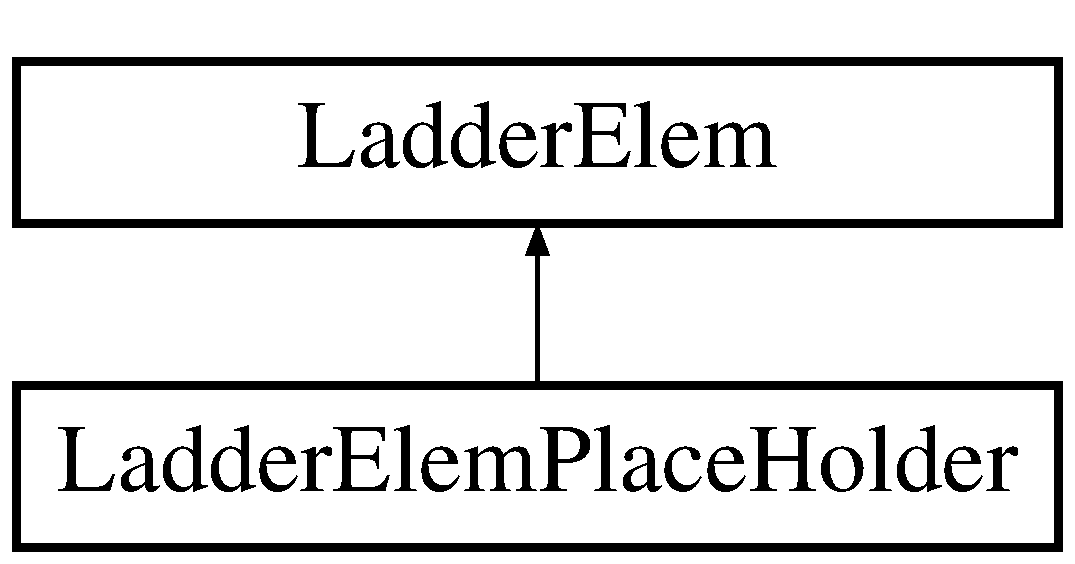
\includegraphics[height=2.000000cm]{class_ladder_elem_place_holder}
\end{center}
\end{figure}
\subsection*{Public Member Functions}
\begin{DoxyCompactItemize}
\item 
\hypertarget{class_ladder_elem_place_holder_ad773e6b5f7972c99558e3e8e74865854}{{\bfseries Ladder\-Elem\-Place\-Holder} (\hyperlink{class_ladder_diagram}{Ladder\-Diagram} $\ast$diagram)}\label{class_ladder_elem_place_holder_ad773e6b5f7972c99558e3e8e74865854}

\item 
\hypertarget{class_ladder_elem_place_holder_a4f49c1b51a99ddfe87b366a7952ec612}{pair$<$ string, string $>$ {\bfseries Draw\-T\-X\-T} (void)}\label{class_ladder_elem_place_holder_a4f49c1b51a99ddfe87b366a7952ec612}

\item 
\hypertarget{class_ladder_elem_place_holder_a779355f5b9328a194ebfa1e24d146ca7}{bool {\bfseries Draw\-G\-U\-I} (bool powered\-Before, void $\ast$data)}\label{class_ladder_elem_place_holder_a779355f5b9328a194ebfa1e24d146ca7}

\item 
\hypertarget{class_ladder_elem_place_holder_a4e14be597ec206b0b4fafb3046aa6f41}{bool {\bfseries Show\-Dialog} (\hyperlink{struct_ladder_context}{Ladder\-Context} context)}\label{class_ladder_elem_place_holder_a4e14be597ec206b0b4fafb3046aa6f41}

\item 
\hypertarget{class_ladder_elem_place_holder_a0cd8af548fc92f7f474863ba01cd36ed}{bool {\bfseries internal\-Generate\-Int\-Code} (\hyperlink{class_int_code}{Int\-Code} \&ic)}\label{class_ladder_elem_place_holder_a0cd8af548fc92f7f474863ba01cd36ed}

\item 
\hypertarget{class_ladder_elem_place_holder_ac5a433c837dcc6c59cc3ab60b318ac1c}{bool {\bfseries Can\-Insert} (\hyperlink{struct_ladder_context}{Ladder\-Context} context)}\label{class_ladder_elem_place_holder_ac5a433c837dcc6c59cc3ab60b318ac1c}

\item 
\hypertarget{class_ladder_elem_place_holder_aedff5783683d8700f36339c8e012224e}{void {\bfseries do\-Post\-Insert} (void)}\label{class_ladder_elem_place_holder_aedff5783683d8700f36339c8e012224e}

\item 
\hypertarget{class_ladder_elem_place_holder_aca181ad5a4e326b8fb3639d968b8329d}{void {\bfseries do\-Post\-Remove} (void)}\label{class_ladder_elem_place_holder_aca181ad5a4e326b8fb3639d968b8329d}

\item 
\hypertarget{class_ladder_elem_place_holder_a0fe4f6fbe4257902a50eaf00ced39328}{int {\bfseries get\-Width\-T\-X\-T} (void)}\label{class_ladder_elem_place_holder_a0fe4f6fbe4257902a50eaf00ced39328}

\item 
\hypertarget{class_ladder_elem_place_holder_a3ab5edcb27986e0e79dc980474b5e79c}{void $\ast$ {\bfseries get\-Properties} (void)}\label{class_ladder_elem_place_holder_a3ab5edcb27986e0e79dc980474b5e79c}

\item 
\hypertarget{class_ladder_elem_place_holder_a9219410c442fa7bef7696364e731af06}{\hyperlink{class_ladder_elem}{Ladder\-Elem} $\ast$ {\bfseries Clone} (\hyperlink{class_ladder_diagram}{Ladder\-Diagram} $\ast$diagram)}\label{class_ladder_elem_place_holder_a9219410c442fa7bef7696364e731af06}

\item 
\hypertarget{class_ladder_elem_place_holder_a3395f986177245b6897b8df50a724d4e}{bool {\bfseries accept\-I\-O} (unsigned long id, e\-Type type)}\label{class_ladder_elem_place_holder_a3395f986177245b6897b8df50a724d4e}

\item 
\hypertarget{class_ladder_elem_place_holder_ab7ca23522d2ad1d85563a0f8d41ffe0c}{void {\bfseries update\-I\-O} (\hyperlink{class_ladder_diagram}{Ladder\-Diagram} $\ast$owner, bool is\-Discard)}\label{class_ladder_elem_place_holder_ab7ca23522d2ad1d85563a0f8d41ffe0c}

\item 
\hypertarget{class_ladder_elem_place_holder_a041685dcac53aade9c75f4d65e9f6dff}{e\-Type {\bfseries get\-Allowed\-Type\-I\-O} (unsigned long id)}\label{class_ladder_elem_place_holder_a041685dcac53aade9c75f4d65e9f6dff}

\item 
\hypertarget{class_ladder_elem_place_holder_aebd38e972925cc453322c42798a18d38}{int {\bfseries Search\-And\-Replace} (unsigned long id\-Search, string s\-New\-Text, bool is\-Replace)}\label{class_ladder_elem_place_holder_aebd38e972925cc453322c42798a18d38}

\item 
\hypertarget{class_ladder_elem_place_holder_ac92b6ed69064ef5ee9d641df389d230a}{bool {\bfseries internal\-Do\-Undo\-Redo} (bool Is\-Undo, bool is\-Discard, \hyperlink{struct_undo_redo_action}{Undo\-Redo\-Action} \&action)}\label{class_ladder_elem_place_holder_ac92b6ed69064ef5ee9d641df389d230a}

\end{DoxyCompactItemize}
\subsection*{Additional Inherited Members}


The documentation for this class was generated from the following files\-:\begin{DoxyCompactItemize}
\item 
F\-:/\-S\-V\-N/\-P\-O\-P\-Tools/Ladder\-Objects.\-h\item 
F\-:/\-S\-V\-N/\-P\-O\-P\-Tools/Ladder\-G\-U\-I.\-cpp\item 
F\-:/\-S\-V\-N/\-P\-O\-P\-Tools/Ladder\-Objects.\-cpp\end{DoxyCompactItemize}

\hypertarget{class_ladder_elem_rand}{\section{Ladder\-Elem\-Rand Class Reference}
\label{class_ladder_elem_rand}\index{Ladder\-Elem\-Rand@{Ladder\-Elem\-Rand}}
}
Inheritance diagram for Ladder\-Elem\-Rand\-:\begin{figure}[H]
\begin{center}
\leavevmode
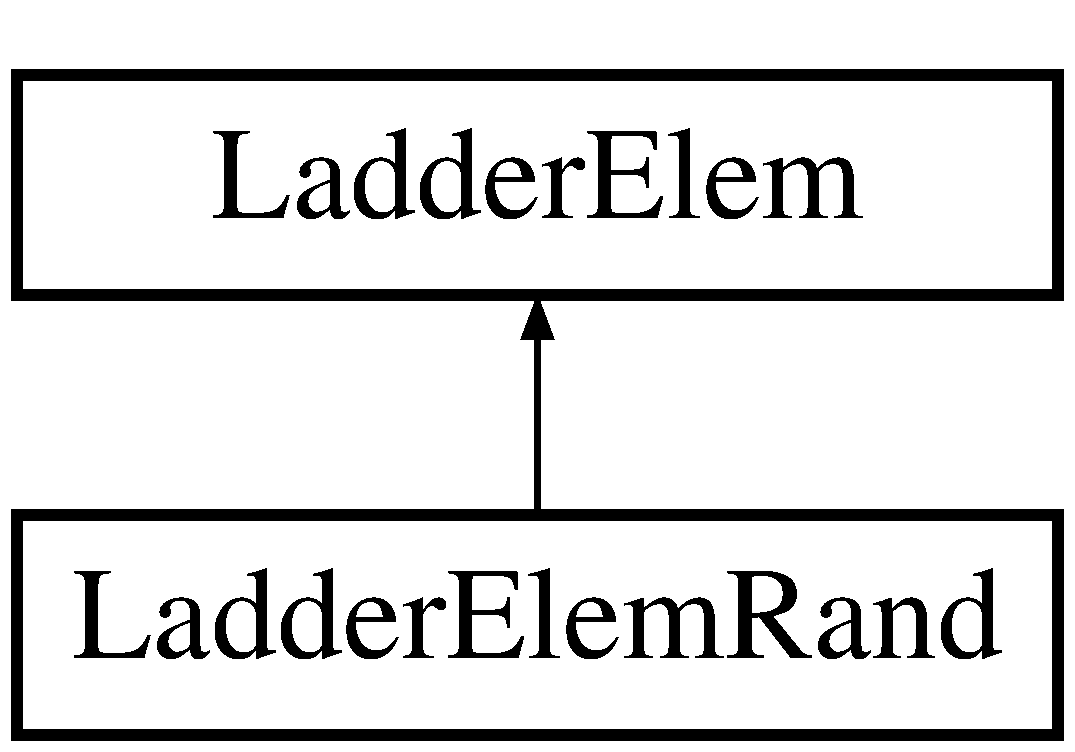
\includegraphics[height=2.000000cm]{class_ladder_elem_rand}
\end{center}
\end{figure}
\subsection*{Public Member Functions}
\begin{DoxyCompactItemize}
\item 
\hypertarget{class_ladder_elem_rand_aa6c386ced93085800a74b355d0181a77}{{\bfseries Ladder\-Elem\-Rand} (\hyperlink{class_ladder_diagram}{Ladder\-Diagram} $\ast$diagram)}\label{class_ladder_elem_rand_aa6c386ced93085800a74b355d0181a77}

\item 
\hypertarget{class_ladder_elem_rand_ac10a5a59c4e2688fe08eddbcb322645b}{pair$<$ string, string $>$ {\bfseries Draw\-T\-X\-T} (void)}\label{class_ladder_elem_rand_ac10a5a59c4e2688fe08eddbcb322645b}

\item 
\hypertarget{class_ladder_elem_rand_a79dc498685cc6bc6e6230cd721cd6617}{bool {\bfseries Draw\-G\-U\-I} (bool powered\-Before, void $\ast$data)}\label{class_ladder_elem_rand_a79dc498685cc6bc6e6230cd721cd6617}

\item 
\hypertarget{class_ladder_elem_rand_af80e8304564cc76f9c6ac3cd1dd6ba6c}{bool {\bfseries Show\-Dialog} (\hyperlink{struct_ladder_context}{Ladder\-Context} context)}\label{class_ladder_elem_rand_af80e8304564cc76f9c6ac3cd1dd6ba6c}

\item 
\hypertarget{class_ladder_elem_rand_ad15f51b48a233092db4cc0513f27a14e}{bool {\bfseries internal\-Generate\-Int\-Code} (\hyperlink{class_int_code}{Int\-Code} \&ic)}\label{class_ladder_elem_rand_ad15f51b48a233092db4cc0513f27a14e}

\item 
\hypertarget{class_ladder_elem_rand_aaddd0e7ff16a0d7cda04ef9d1b0a0853}{void $\ast$ {\bfseries get\-Properties} (void)}\label{class_ladder_elem_rand_aaddd0e7ff16a0d7cda04ef9d1b0a0853}

\item 
\hypertarget{class_ladder_elem_rand_a4cdc5b7c5c9a3906dff228f3110962b7}{bool {\bfseries Can\-Insert} (\hyperlink{struct_ladder_context}{Ladder\-Context} context)}\label{class_ladder_elem_rand_a4cdc5b7c5c9a3906dff228f3110962b7}

\item 
\hypertarget{class_ladder_elem_rand_a298b80c6faf1a956a1ca3a04fed5f540}{void {\bfseries do\-Post\-Insert} (void)}\label{class_ladder_elem_rand_a298b80c6faf1a956a1ca3a04fed5f540}

\item 
\hypertarget{class_ladder_elem_rand_ac47d8628664c6e91c4cc58536ff87e4c}{void {\bfseries do\-Post\-Remove} (void)}\label{class_ladder_elem_rand_ac47d8628664c6e91c4cc58536ff87e4c}

\item 
\hypertarget{class_ladder_elem_rand_ae0af4377973cb977fe635604f8de0c4d}{int {\bfseries get\-Width\-T\-X\-T} (void)}\label{class_ladder_elem_rand_ae0af4377973cb977fe635604f8de0c4d}

\item 
\hypertarget{class_ladder_elem_rand_a63ba163d93477442e71c17d0fd390807}{\hyperlink{class_ladder_elem}{Ladder\-Elem} $\ast$ {\bfseries Clone} (\hyperlink{class_ladder_diagram}{Ladder\-Diagram} $\ast$diagram)}\label{class_ladder_elem_rand_a63ba163d93477442e71c17d0fd390807}

\item 
\hypertarget{class_ladder_elem_rand_a30e8538b008229a73db0749a5a623014}{bool {\bfseries accept\-I\-O} (unsigned long id, e\-Type type)}\label{class_ladder_elem_rand_a30e8538b008229a73db0749a5a623014}

\item 
\hypertarget{class_ladder_elem_rand_a6d2bbdf8e6bdc6d5f4a528259133ba1b}{void {\bfseries update\-I\-O} (\hyperlink{class_ladder_diagram}{Ladder\-Diagram} $\ast$owner, bool is\-Discard)}\label{class_ladder_elem_rand_a6d2bbdf8e6bdc6d5f4a528259133ba1b}

\item 
\hypertarget{class_ladder_elem_rand_a0c0cfb97c91de2d4c2d11b3b4f088e16}{e\-Type {\bfseries get\-Allowed\-Type\-I\-O} (unsigned long id)}\label{class_ladder_elem_rand_a0c0cfb97c91de2d4c2d11b3b4f088e16}

\item 
\hypertarget{class_ladder_elem_rand_ab36be1a4089ab43b83c9deed4db49718}{int {\bfseries Search\-And\-Replace} (unsigned long id\-Search, string s\-New\-Text, bool is\-Replace)}\label{class_ladder_elem_rand_ab36be1a4089ab43b83c9deed4db49718}

\item 
\hypertarget{class_ladder_elem_rand_a1e2be78811147a042f39fec0422b9386}{bool {\bfseries internal\-Do\-Undo\-Redo} (bool Is\-Undo, bool is\-Discard, \hyperlink{struct_undo_redo_action}{Undo\-Redo\-Action} \&action)}\label{class_ladder_elem_rand_a1e2be78811147a042f39fec0422b9386}

\end{DoxyCompactItemize}
\subsection*{Additional Inherited Members}


The documentation for this class was generated from the following files\-:\begin{DoxyCompactItemize}
\item 
F\-:/\-S\-V\-N/\-P\-O\-P\-Tools/Ladder\-Objects.\-h\item 
F\-:/\-S\-V\-N/\-P\-O\-P\-Tools/Ladder\-G\-U\-I.\-cpp\item 
F\-:/\-S\-V\-N/\-P\-O\-P\-Tools/Ladder\-Objects.\-cpp\end{DoxyCompactItemize}

\hypertarget{struct_ladder_elem_rand_prop}{\section{Ladder\-Elem\-Rand\-Prop Struct Reference}
\label{struct_ladder_elem_rand_prop}\index{Ladder\-Elem\-Rand\-Prop@{Ladder\-Elem\-Rand\-Prop}}
}
\subsection*{Public Attributes}
\begin{DoxyCompactItemize}
\item 
\hypertarget{struct_ladder_elem_rand_prop_ac3c90778036fe78eb883eaa8ee3850a6}{pair$<$ unsigned long, int $>$ {\bfseries id\-Var}}\label{struct_ladder_elem_rand_prop_ac3c90778036fe78eb883eaa8ee3850a6}

\item 
\hypertarget{struct_ladder_elem_rand_prop_a3bc25fbeef0b2833360c54bd3194a7b7}{pair$<$ unsigned long, int $>$ {\bfseries id\-Min}}\label{struct_ladder_elem_rand_prop_a3bc25fbeef0b2833360c54bd3194a7b7}

\item 
\hypertarget{struct_ladder_elem_rand_prop_a90f21a722a445a50511be722e2bdf95e}{pair$<$ unsigned long, int $>$ {\bfseries id\-Max}}\label{struct_ladder_elem_rand_prop_a90f21a722a445a50511be722e2bdf95e}

\end{DoxyCompactItemize}


The documentation for this struct was generated from the following file\-:\begin{DoxyCompactItemize}
\item 
F\-:/\-S\-V\-N/\-P\-O\-P\-Tools/Ladder\-Objects.\-h\end{DoxyCompactItemize}

\hypertarget{class_ladder_elem_read_adc}{\section{Ladder\-Elem\-Read\-Adc Class Reference}
\label{class_ladder_elem_read_adc}\index{Ladder\-Elem\-Read\-Adc@{Ladder\-Elem\-Read\-Adc}}
}
Inheritance diagram for Ladder\-Elem\-Read\-Adc\-:\begin{figure}[H]
\begin{center}
\leavevmode
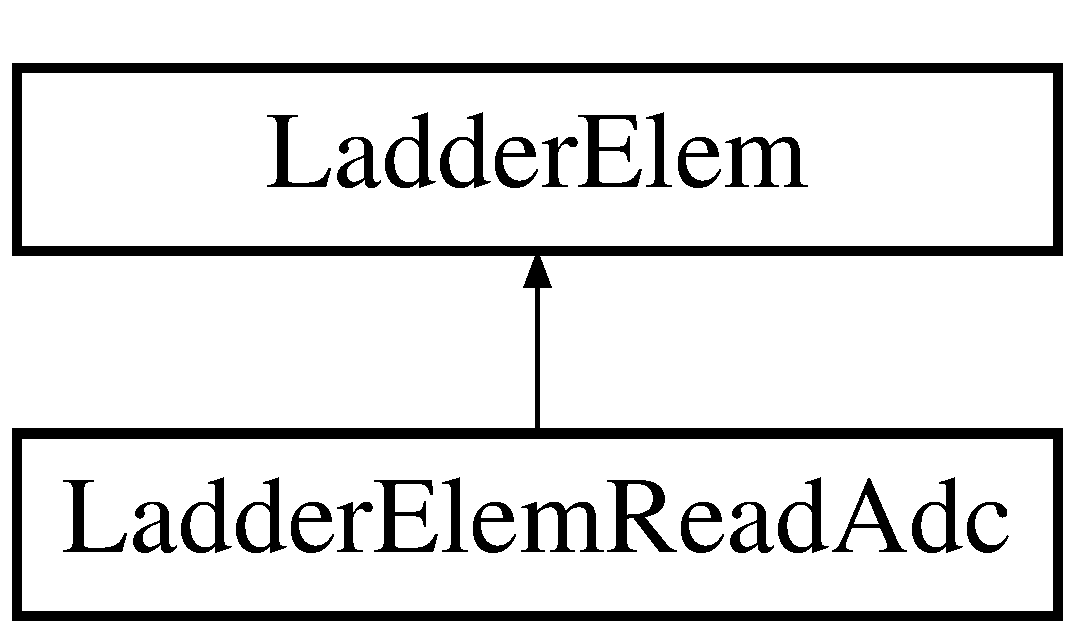
\includegraphics[height=2.000000cm]{class_ladder_elem_read_adc}
\end{center}
\end{figure}
\subsection*{Public Member Functions}
\begin{DoxyCompactItemize}
\item 
\hypertarget{class_ladder_elem_read_adc_a609a8fd02633a47512f165c44daf32cb}{{\bfseries Ladder\-Elem\-Read\-Adc} (\hyperlink{class_ladder_diagram}{Ladder\-Diagram} $\ast$diagram)}\label{class_ladder_elem_read_adc_a609a8fd02633a47512f165c44daf32cb}

\item 
\hypertarget{class_ladder_elem_read_adc_ae695f6bfca57f4c06188c80738a46943}{pair$<$ string, string $>$ {\bfseries Draw\-T\-X\-T} (void)}\label{class_ladder_elem_read_adc_ae695f6bfca57f4c06188c80738a46943}

\item 
\hypertarget{class_ladder_elem_read_adc_ad6c8eeecd10ebea4f7863fb817a057a1}{bool {\bfseries Draw\-G\-U\-I} (bool powered\-Before, void $\ast$data)}\label{class_ladder_elem_read_adc_ad6c8eeecd10ebea4f7863fb817a057a1}

\item 
\hypertarget{class_ladder_elem_read_adc_ac15b42cd8042c2177f1b56a1a810f181}{bool {\bfseries Show\-Dialog} (\hyperlink{struct_ladder_context}{Ladder\-Context} context)}\label{class_ladder_elem_read_adc_ac15b42cd8042c2177f1b56a1a810f181}

\item 
\hypertarget{class_ladder_elem_read_adc_a6ca250da8838f8d222ccbb630e350ce2}{bool {\bfseries internal\-Generate\-Int\-Code} (\hyperlink{class_int_code}{Int\-Code} \&ic)}\label{class_ladder_elem_read_adc_a6ca250da8838f8d222ccbb630e350ce2}

\item 
\hypertarget{class_ladder_elem_read_adc_a5e16d53117f0665d4ee97d63407c9cea}{void $\ast$ {\bfseries get\-Properties} (void)}\label{class_ladder_elem_read_adc_a5e16d53117f0665d4ee97d63407c9cea}

\item 
\hypertarget{class_ladder_elem_read_adc_a443d7080a2dad22755c6503d49b3358e}{bool {\bfseries Can\-Insert} (\hyperlink{struct_ladder_context}{Ladder\-Context} context)}\label{class_ladder_elem_read_adc_a443d7080a2dad22755c6503d49b3358e}

\item 
\hypertarget{class_ladder_elem_read_adc_a8daa7f694c4b1de2114a8a48ed602d81}{void {\bfseries do\-Post\-Insert} (void)}\label{class_ladder_elem_read_adc_a8daa7f694c4b1de2114a8a48ed602d81}

\item 
\hypertarget{class_ladder_elem_read_adc_afe529dac0ea797f700c48ec8d71c2697}{void {\bfseries do\-Post\-Remove} (void)}\label{class_ladder_elem_read_adc_afe529dac0ea797f700c48ec8d71c2697}

\item 
\hypertarget{class_ladder_elem_read_adc_a3b7dc40610beb9fadf3878d6cfdca554}{int {\bfseries get\-Width\-T\-X\-T} (void)}\label{class_ladder_elem_read_adc_a3b7dc40610beb9fadf3878d6cfdca554}

\item 
\hypertarget{class_ladder_elem_read_adc_a4bbc61e289f0594f044bc7dc41d67ff4}{\hyperlink{class_ladder_elem}{Ladder\-Elem} $\ast$ {\bfseries Clone} (\hyperlink{class_ladder_diagram}{Ladder\-Diagram} $\ast$diagram)}\label{class_ladder_elem_read_adc_a4bbc61e289f0594f044bc7dc41d67ff4}

\item 
\hypertarget{class_ladder_elem_read_adc_a69d3522332857eb6b4badf210a7c226b}{bool {\bfseries accept\-I\-O} (unsigned long id, e\-Type type)}\label{class_ladder_elem_read_adc_a69d3522332857eb6b4badf210a7c226b}

\item 
\hypertarget{class_ladder_elem_read_adc_a9554b3f53438de5f76db3235c79bb097}{void {\bfseries update\-I\-O} (\hyperlink{class_ladder_diagram}{Ladder\-Diagram} $\ast$owner, bool is\-Discard)}\label{class_ladder_elem_read_adc_a9554b3f53438de5f76db3235c79bb097}

\item 
\hypertarget{class_ladder_elem_read_adc_a4eaa5b0ffa5e6a527c826c05d3dac0ed}{e\-Type {\bfseries get\-Allowed\-Type\-I\-O} (unsigned long id)}\label{class_ladder_elem_read_adc_a4eaa5b0ffa5e6a527c826c05d3dac0ed}

\item 
\hypertarget{class_ladder_elem_read_adc_a766f294465a0c5abca1b8b467040ad8b}{int {\bfseries Search\-And\-Replace} (unsigned long id\-Search, string s\-New\-Text, bool is\-Replace)}\label{class_ladder_elem_read_adc_a766f294465a0c5abca1b8b467040ad8b}

\item 
\hypertarget{class_ladder_elem_read_adc_aa4aa15d568073efe5cc711a528906948}{bool {\bfseries internal\-Do\-Undo\-Redo} (bool Is\-Undo, bool is\-Discard, \hyperlink{struct_undo_redo_action}{Undo\-Redo\-Action} \&action)}\label{class_ladder_elem_read_adc_aa4aa15d568073efe5cc711a528906948}

\end{DoxyCompactItemize}
\subsection*{Additional Inherited Members}


The documentation for this class was generated from the following files\-:\begin{DoxyCompactItemize}
\item 
F\-:/\-S\-V\-N/\-P\-O\-P\-Tools/Ladder\-Objects.\-h\item 
F\-:/\-S\-V\-N/\-P\-O\-P\-Tools/Ladder\-G\-U\-I.\-cpp\item 
F\-:/\-S\-V\-N/\-P\-O\-P\-Tools/Ladder\-Objects.\-cpp\end{DoxyCompactItemize}

\hypertarget{struct_ladder_elem_read_adc_prop}{\section{Ladder\-Elem\-Read\-Adc\-Prop Struct Reference}
\label{struct_ladder_elem_read_adc_prop}\index{Ladder\-Elem\-Read\-Adc\-Prop@{Ladder\-Elem\-Read\-Adc\-Prop}}
}
\subsection*{Public Attributes}
\begin{DoxyCompactItemize}
\item 
\hypertarget{struct_ladder_elem_read_adc_prop_a4d152c6dd348f7a0cb5788d9da5635b8}{pair$<$ unsigned long, int $>$ {\bfseries id\-Name}}\label{struct_ladder_elem_read_adc_prop_a4d152c6dd348f7a0cb5788d9da5635b8}

\end{DoxyCompactItemize}


The documentation for this struct was generated from the following file\-:\begin{DoxyCompactItemize}
\item 
F\-:/\-S\-V\-N/\-P\-O\-P\-Tools/Ladder\-Objects.\-h\end{DoxyCompactItemize}

\hypertarget{class_ladder_elem_read_enc}{\section{Ladder\-Elem\-Read\-Enc Class Reference}
\label{class_ladder_elem_read_enc}\index{Ladder\-Elem\-Read\-Enc@{Ladder\-Elem\-Read\-Enc}}
}
Inheritance diagram for Ladder\-Elem\-Read\-Enc\-:\begin{figure}[H]
\begin{center}
\leavevmode
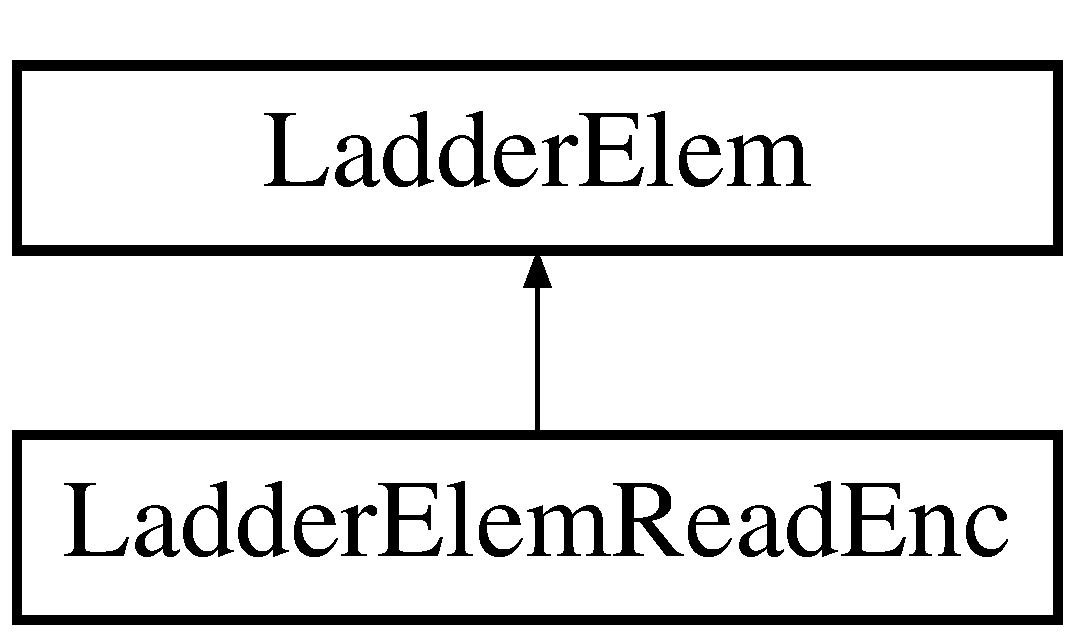
\includegraphics[height=2.000000cm]{class_ladder_elem_read_enc}
\end{center}
\end{figure}
\subsection*{Public Member Functions}
\begin{DoxyCompactItemize}
\item 
\hypertarget{class_ladder_elem_read_enc_a38e166df9fde25275282b9a2ac6e041f}{{\bfseries Ladder\-Elem\-Read\-Enc} (\hyperlink{class_ladder_diagram}{Ladder\-Diagram} $\ast$diagram)}\label{class_ladder_elem_read_enc_a38e166df9fde25275282b9a2ac6e041f}

\item 
\hypertarget{class_ladder_elem_read_enc_a555776a3da805a596ce85c1a48a47bc6}{pair$<$ string, string $>$ {\bfseries Draw\-T\-X\-T} (void)}\label{class_ladder_elem_read_enc_a555776a3da805a596ce85c1a48a47bc6}

\item 
\hypertarget{class_ladder_elem_read_enc_a1da6125cee20746467021638136790d0}{bool {\bfseries Draw\-G\-U\-I} (bool powered\-Before, void $\ast$data)}\label{class_ladder_elem_read_enc_a1da6125cee20746467021638136790d0}

\item 
\hypertarget{class_ladder_elem_read_enc_adb875f9629e34c2c6a321bce7691dc58}{bool {\bfseries Show\-Dialog} (\hyperlink{struct_ladder_context}{Ladder\-Context} context)}\label{class_ladder_elem_read_enc_adb875f9629e34c2c6a321bce7691dc58}

\item 
\hypertarget{class_ladder_elem_read_enc_ab9ef41c7c158a60343a3339d8be4876a}{bool {\bfseries internal\-Generate\-Int\-Code} (\hyperlink{class_int_code}{Int\-Code} \&ic)}\label{class_ladder_elem_read_enc_ab9ef41c7c158a60343a3339d8be4876a}

\item 
\hypertarget{class_ladder_elem_read_enc_a9be752bf18066f878ca00c80493f8b84}{void $\ast$ {\bfseries get\-Properties} (void)}\label{class_ladder_elem_read_enc_a9be752bf18066f878ca00c80493f8b84}

\item 
\hypertarget{class_ladder_elem_read_enc_a7c4be7738c7b33a10a7ed284c7b249a3}{bool {\bfseries Can\-Insert} (\hyperlink{struct_ladder_context}{Ladder\-Context} context)}\label{class_ladder_elem_read_enc_a7c4be7738c7b33a10a7ed284c7b249a3}

\item 
\hypertarget{class_ladder_elem_read_enc_ae5838b3713f0bffe30c59fc728a0683e}{void {\bfseries do\-Post\-Insert} (void)}\label{class_ladder_elem_read_enc_ae5838b3713f0bffe30c59fc728a0683e}

\item 
\hypertarget{class_ladder_elem_read_enc_a3720a5eb533e22c517f3505488df7975}{void {\bfseries do\-Post\-Remove} (void)}\label{class_ladder_elem_read_enc_a3720a5eb533e22c517f3505488df7975}

\item 
\hypertarget{class_ladder_elem_read_enc_a4e14724716242f3a1547e4f21f498a33}{int {\bfseries get\-Width\-T\-X\-T} (void)}\label{class_ladder_elem_read_enc_a4e14724716242f3a1547e4f21f498a33}

\item 
\hypertarget{class_ladder_elem_read_enc_ad1f22de26a6aa2582611fcbd1d45d390}{\hyperlink{class_ladder_elem}{Ladder\-Elem} $\ast$ {\bfseries Clone} (\hyperlink{class_ladder_diagram}{Ladder\-Diagram} $\ast$diagram)}\label{class_ladder_elem_read_enc_ad1f22de26a6aa2582611fcbd1d45d390}

\item 
\hypertarget{class_ladder_elem_read_enc_a80deac2308468f134c6092fcb6d22efc}{bool {\bfseries accept\-I\-O} (unsigned long id, e\-Type type)}\label{class_ladder_elem_read_enc_a80deac2308468f134c6092fcb6d22efc}

\item 
\hypertarget{class_ladder_elem_read_enc_a2395de5177ff17d53df7bc3b5b2788dc}{void {\bfseries update\-I\-O} (\hyperlink{class_ladder_diagram}{Ladder\-Diagram} $\ast$owner, bool is\-Discard)}\label{class_ladder_elem_read_enc_a2395de5177ff17d53df7bc3b5b2788dc}

\item 
\hypertarget{class_ladder_elem_read_enc_a8499c6ced8534d634f1d71f2bce0ec98}{e\-Type {\bfseries get\-Allowed\-Type\-I\-O} (unsigned long id)}\label{class_ladder_elem_read_enc_a8499c6ced8534d634f1d71f2bce0ec98}

\item 
\hypertarget{class_ladder_elem_read_enc_adaea501f283f4f71b164e6ce4fa1cb0c}{int {\bfseries Search\-And\-Replace} (unsigned long id\-Search, string s\-New\-Text, bool is\-Replace)}\label{class_ladder_elem_read_enc_adaea501f283f4f71b164e6ce4fa1cb0c}

\item 
\hypertarget{class_ladder_elem_read_enc_ac90c6469c37ab6cea4053c466088c47e}{bool {\bfseries internal\-Do\-Undo\-Redo} (bool Is\-Undo, bool is\-Discard, \hyperlink{struct_undo_redo_action}{Undo\-Redo\-Action} \&action)}\label{class_ladder_elem_read_enc_ac90c6469c37ab6cea4053c466088c47e}

\end{DoxyCompactItemize}
\subsection*{Additional Inherited Members}


The documentation for this class was generated from the following files\-:\begin{DoxyCompactItemize}
\item 
F\-:/\-S\-V\-N/\-P\-O\-P\-Tools/Ladder\-Objects.\-h\item 
F\-:/\-S\-V\-N/\-P\-O\-P\-Tools/Ladder\-G\-U\-I.\-cpp\item 
F\-:/\-S\-V\-N/\-P\-O\-P\-Tools/Ladder\-Objects.\-cpp\end{DoxyCompactItemize}

\hypertarget{struct_ladder_elem_read_enc_prop}{\section{Ladder\-Elem\-Read\-Enc\-Prop Struct Reference}
\label{struct_ladder_elem_read_enc_prop}\index{Ladder\-Elem\-Read\-Enc\-Prop@{Ladder\-Elem\-Read\-Enc\-Prop}}
}
\subsection*{Public Attributes}
\begin{DoxyCompactItemize}
\item 
\hypertarget{struct_ladder_elem_read_enc_prop_a0448fda3433e237646f9732103af358d}{pair$<$ unsigned long, int $>$ {\bfseries id\-Name}}\label{struct_ladder_elem_read_enc_prop_a0448fda3433e237646f9732103af358d}

\end{DoxyCompactItemize}


The documentation for this struct was generated from the following file\-:\begin{DoxyCompactItemize}
\item 
F\-:/\-S\-V\-N/\-P\-O\-P\-Tools/Ladder\-Objects.\-h\end{DoxyCompactItemize}

\hypertarget{class_ladder_elem_reset}{\section{Ladder\-Elem\-Reset Class Reference}
\label{class_ladder_elem_reset}\index{Ladder\-Elem\-Reset@{Ladder\-Elem\-Reset}}
}
Inheritance diagram for Ladder\-Elem\-Reset\-:\begin{figure}[H]
\begin{center}
\leavevmode
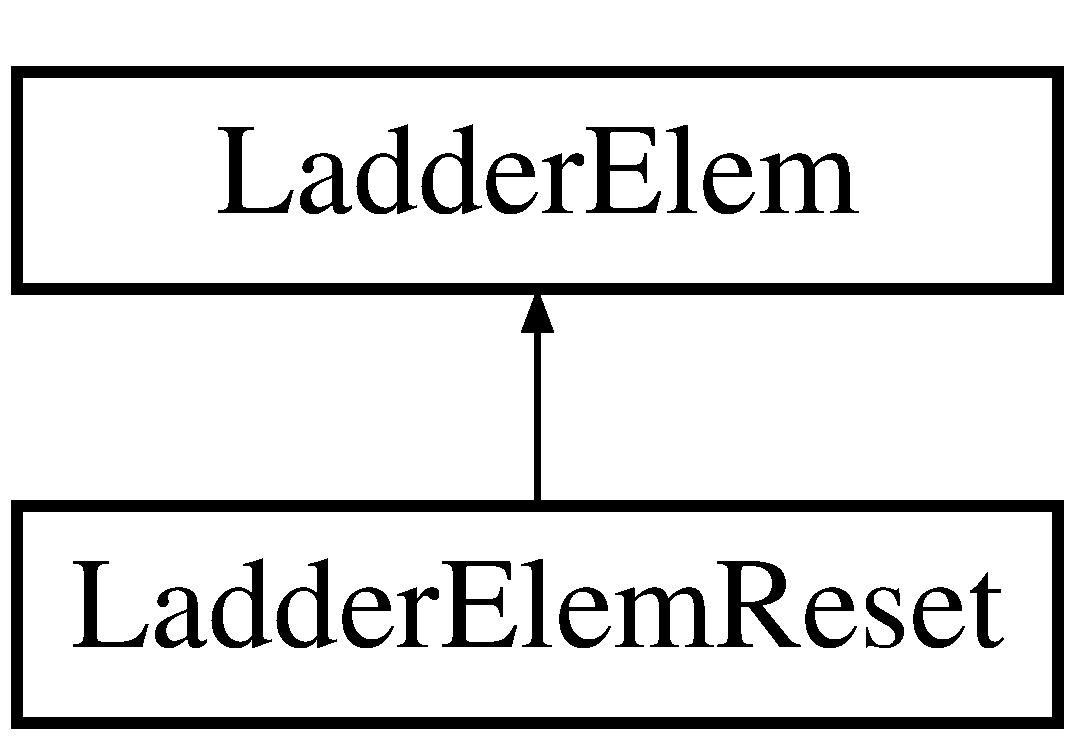
\includegraphics[height=2.000000cm]{class_ladder_elem_reset}
\end{center}
\end{figure}
\subsection*{Public Member Functions}
\begin{DoxyCompactItemize}
\item 
\hypertarget{class_ladder_elem_reset_afb99ea838eac20c7d994198b060c54a1}{{\bfseries Ladder\-Elem\-Reset} (\hyperlink{class_ladder_diagram}{Ladder\-Diagram} $\ast$diagram)}\label{class_ladder_elem_reset_afb99ea838eac20c7d994198b060c54a1}

\item 
\hypertarget{class_ladder_elem_reset_a34c8fb5eea26687095d5b2ff998581e8}{pair$<$ string, string $>$ {\bfseries Draw\-T\-X\-T} (void)}\label{class_ladder_elem_reset_a34c8fb5eea26687095d5b2ff998581e8}

\item 
\hypertarget{class_ladder_elem_reset_a0fb98ff182314c9b714e44819ee91966}{bool {\bfseries Draw\-G\-U\-I} (bool powered\-Before, void $\ast$data)}\label{class_ladder_elem_reset_a0fb98ff182314c9b714e44819ee91966}

\item 
\hypertarget{class_ladder_elem_reset_ae2ebc092fccce13c83cae4eb046c0b53}{bool {\bfseries Show\-Dialog} (\hyperlink{struct_ladder_context}{Ladder\-Context} context)}\label{class_ladder_elem_reset_ae2ebc092fccce13c83cae4eb046c0b53}

\item 
\hypertarget{class_ladder_elem_reset_ad24d9121e6ebcdfb0ac9c633e9430b4b}{bool {\bfseries internal\-Generate\-Int\-Code} (\hyperlink{class_int_code}{Int\-Code} \&ic)}\label{class_ladder_elem_reset_ad24d9121e6ebcdfb0ac9c633e9430b4b}

\item 
\hypertarget{class_ladder_elem_reset_aa4c19c79014bd821612a013a3934d766}{void $\ast$ {\bfseries get\-Properties} (void)}\label{class_ladder_elem_reset_aa4c19c79014bd821612a013a3934d766}

\item 
\hypertarget{class_ladder_elem_reset_a8f335b390d2eaca8151799d41ed92566}{bool {\bfseries Can\-Insert} (\hyperlink{struct_ladder_context}{Ladder\-Context} context)}\label{class_ladder_elem_reset_a8f335b390d2eaca8151799d41ed92566}

\item 
\hypertarget{class_ladder_elem_reset_a41053295a1edcf6fe1e1c93b77554159}{void {\bfseries do\-Post\-Insert} (void)}\label{class_ladder_elem_reset_a41053295a1edcf6fe1e1c93b77554159}

\item 
\hypertarget{class_ladder_elem_reset_a18629fe94cd2f71539ff63b14e5e80cc}{void {\bfseries do\-Post\-Remove} (void)}\label{class_ladder_elem_reset_a18629fe94cd2f71539ff63b14e5e80cc}

\item 
\hypertarget{class_ladder_elem_reset_a261a7ca998217f2a748ee1bb07982f0e}{int {\bfseries get\-Width\-T\-X\-T} (void)}\label{class_ladder_elem_reset_a261a7ca998217f2a748ee1bb07982f0e}

\item 
\hypertarget{class_ladder_elem_reset_af142d0a3d56de53162db501a1a2da190}{\hyperlink{class_ladder_elem}{Ladder\-Elem} $\ast$ {\bfseries Clone} (\hyperlink{class_ladder_diagram}{Ladder\-Diagram} $\ast$diagram)}\label{class_ladder_elem_reset_af142d0a3d56de53162db501a1a2da190}

\item 
\hypertarget{class_ladder_elem_reset_a1ac40f5ff86174681317605100aea07f}{bool {\bfseries accept\-I\-O} (unsigned long id, e\-Type type)}\label{class_ladder_elem_reset_a1ac40f5ff86174681317605100aea07f}

\item 
\hypertarget{class_ladder_elem_reset_abc54cbfbea4887801ce294f4e93114cb}{void {\bfseries update\-I\-O} (\hyperlink{class_ladder_diagram}{Ladder\-Diagram} $\ast$owner, bool is\-Discard)}\label{class_ladder_elem_reset_abc54cbfbea4887801ce294f4e93114cb}

\item 
\hypertarget{class_ladder_elem_reset_a09945da7463d6ac25049715a794c265d}{e\-Type {\bfseries get\-Allowed\-Type\-I\-O} (unsigned long id)}\label{class_ladder_elem_reset_a09945da7463d6ac25049715a794c265d}

\item 
\hypertarget{class_ladder_elem_reset_a2a05d3fa13f197fcc0cfeb3ee342db07}{int {\bfseries Search\-And\-Replace} (unsigned long id\-Search, string s\-New\-Text, bool is\-Replace)}\label{class_ladder_elem_reset_a2a05d3fa13f197fcc0cfeb3ee342db07}

\item 
\hypertarget{class_ladder_elem_reset_a67e70c1ec2becb78676d48f5c42e443c}{bool {\bfseries internal\-Do\-Undo\-Redo} (bool Is\-Undo, bool is\-Discard, \hyperlink{struct_undo_redo_action}{Undo\-Redo\-Action} \&action)}\label{class_ladder_elem_reset_a67e70c1ec2becb78676d48f5c42e443c}

\end{DoxyCompactItemize}
\subsection*{Additional Inherited Members}


The documentation for this class was generated from the following files\-:\begin{DoxyCompactItemize}
\item 
F\-:/\-S\-V\-N/\-P\-O\-P\-Tools/Ladder\-Objects.\-h\item 
F\-:/\-S\-V\-N/\-P\-O\-P\-Tools/Ladder\-G\-U\-I.\-cpp\item 
F\-:/\-S\-V\-N/\-P\-O\-P\-Tools/Ladder\-Objects.\-cpp\end{DoxyCompactItemize}

\hypertarget{class_ladder_elem_reset_enc}{\section{Ladder\-Elem\-Reset\-Enc Class Reference}
\label{class_ladder_elem_reset_enc}\index{Ladder\-Elem\-Reset\-Enc@{Ladder\-Elem\-Reset\-Enc}}
}
Inheritance diagram for Ladder\-Elem\-Reset\-Enc\-:\begin{figure}[H]
\begin{center}
\leavevmode
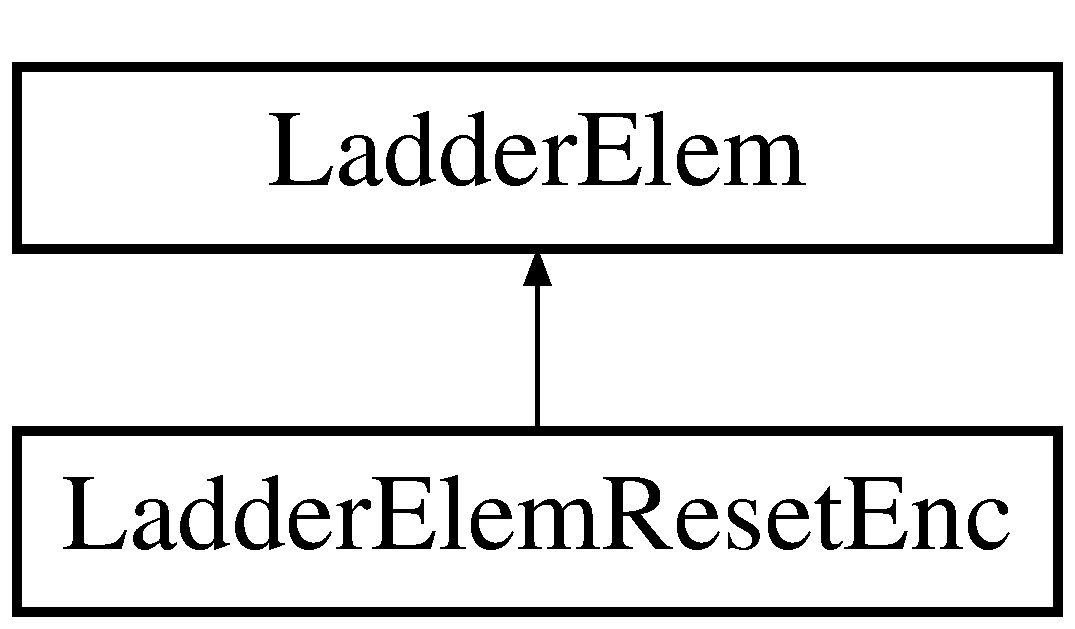
\includegraphics[height=2.000000cm]{class_ladder_elem_reset_enc}
\end{center}
\end{figure}
\subsection*{Public Member Functions}
\begin{DoxyCompactItemize}
\item 
\hypertarget{class_ladder_elem_reset_enc_ab897cd09a5b7f9305c7ffea80297d90d}{{\bfseries Ladder\-Elem\-Reset\-Enc} (\hyperlink{class_ladder_diagram}{Ladder\-Diagram} $\ast$diagram)}\label{class_ladder_elem_reset_enc_ab897cd09a5b7f9305c7ffea80297d90d}

\item 
\hypertarget{class_ladder_elem_reset_enc_ac6ed1eb5730a80e06be9bd65545e6b01}{pair$<$ string, string $>$ {\bfseries Draw\-T\-X\-T} (void)}\label{class_ladder_elem_reset_enc_ac6ed1eb5730a80e06be9bd65545e6b01}

\item 
\hypertarget{class_ladder_elem_reset_enc_a34f720b20dd89328d702d9d35f421f41}{bool {\bfseries Draw\-G\-U\-I} (bool powered\-Before, void $\ast$data)}\label{class_ladder_elem_reset_enc_a34f720b20dd89328d702d9d35f421f41}

\item 
\hypertarget{class_ladder_elem_reset_enc_a5b03e3c8861f2f343a1ffd29d9d45a50}{bool {\bfseries Show\-Dialog} (\hyperlink{struct_ladder_context}{Ladder\-Context} context)}\label{class_ladder_elem_reset_enc_a5b03e3c8861f2f343a1ffd29d9d45a50}

\item 
\hypertarget{class_ladder_elem_reset_enc_a8bfd1caac166cd5e310d1430b58ea2f5}{bool {\bfseries internal\-Generate\-Int\-Code} (\hyperlink{class_int_code}{Int\-Code} \&ic)}\label{class_ladder_elem_reset_enc_a8bfd1caac166cd5e310d1430b58ea2f5}

\item 
\hypertarget{class_ladder_elem_reset_enc_a9f2362920a6e9cf0d1c8e0f1beaf558b}{void $\ast$ {\bfseries get\-Properties} (void)}\label{class_ladder_elem_reset_enc_a9f2362920a6e9cf0d1c8e0f1beaf558b}

\item 
\hypertarget{class_ladder_elem_reset_enc_a7fe1b26ce9e31b5a2f8274b7516fcf8f}{bool {\bfseries Can\-Insert} (\hyperlink{struct_ladder_context}{Ladder\-Context} context)}\label{class_ladder_elem_reset_enc_a7fe1b26ce9e31b5a2f8274b7516fcf8f}

\item 
\hypertarget{class_ladder_elem_reset_enc_a5de7a1d6dc9721a7f282ffdcce9240fd}{void {\bfseries do\-Post\-Insert} (void)}\label{class_ladder_elem_reset_enc_a5de7a1d6dc9721a7f282ffdcce9240fd}

\item 
\hypertarget{class_ladder_elem_reset_enc_ae899aada68efaa36150e47526919815e}{void {\bfseries do\-Post\-Remove} (void)}\label{class_ladder_elem_reset_enc_ae899aada68efaa36150e47526919815e}

\item 
\hypertarget{class_ladder_elem_reset_enc_a7ae57f186eb422c761340bc41390f637}{int {\bfseries get\-Width\-T\-X\-T} (void)}\label{class_ladder_elem_reset_enc_a7ae57f186eb422c761340bc41390f637}

\item 
\hypertarget{class_ladder_elem_reset_enc_acd5899ad911931ee3ac140147a544c3f}{\hyperlink{class_ladder_elem}{Ladder\-Elem} $\ast$ {\bfseries Clone} (\hyperlink{class_ladder_diagram}{Ladder\-Diagram} $\ast$diagram)}\label{class_ladder_elem_reset_enc_acd5899ad911931ee3ac140147a544c3f}

\item 
\hypertarget{class_ladder_elem_reset_enc_abde1e3c1e7ff27a0e48361748996f8c4}{bool {\bfseries accept\-I\-O} (unsigned long id, e\-Type type)}\label{class_ladder_elem_reset_enc_abde1e3c1e7ff27a0e48361748996f8c4}

\item 
\hypertarget{class_ladder_elem_reset_enc_ae46c9b5e27e4eace96063f73a9991e10}{void {\bfseries update\-I\-O} (\hyperlink{class_ladder_diagram}{Ladder\-Diagram} $\ast$owner, bool is\-Discard)}\label{class_ladder_elem_reset_enc_ae46c9b5e27e4eace96063f73a9991e10}

\item 
\hypertarget{class_ladder_elem_reset_enc_ac6e3a963fb1df5f918c2391ee36a23b8}{e\-Type {\bfseries get\-Allowed\-Type\-I\-O} (unsigned long id)}\label{class_ladder_elem_reset_enc_ac6e3a963fb1df5f918c2391ee36a23b8}

\item 
\hypertarget{class_ladder_elem_reset_enc_a47b6598190c6155d99e638e0bfd04d40}{int {\bfseries Search\-And\-Replace} (unsigned long id\-Search, string s\-New\-Text, bool is\-Replace)}\label{class_ladder_elem_reset_enc_a47b6598190c6155d99e638e0bfd04d40}

\item 
\hypertarget{class_ladder_elem_reset_enc_a5e44425d8070a3fcace4b4cc6767e485}{bool {\bfseries internal\-Do\-Undo\-Redo} (bool Is\-Undo, bool is\-Discard, \hyperlink{struct_undo_redo_action}{Undo\-Redo\-Action} \&action)}\label{class_ladder_elem_reset_enc_a5e44425d8070a3fcace4b4cc6767e485}

\end{DoxyCompactItemize}
\subsection*{Additional Inherited Members}


The documentation for this class was generated from the following files\-:\begin{DoxyCompactItemize}
\item 
F\-:/\-S\-V\-N/\-P\-O\-P\-Tools/Ladder\-Objects.\-h\item 
F\-:/\-S\-V\-N/\-P\-O\-P\-Tools/Ladder\-G\-U\-I.\-cpp\item 
F\-:/\-S\-V\-N/\-P\-O\-P\-Tools/Ladder\-Objects.\-cpp\end{DoxyCompactItemize}

\hypertarget{struct_ladder_elem_reset_enc_prop}{\section{Ladder\-Elem\-Reset\-Enc\-Prop Struct Reference}
\label{struct_ladder_elem_reset_enc_prop}\index{Ladder\-Elem\-Reset\-Enc\-Prop@{Ladder\-Elem\-Reset\-Enc\-Prop}}
}
\subsection*{Public Attributes}
\begin{DoxyCompactItemize}
\item 
\hypertarget{struct_ladder_elem_reset_enc_prop_a7b1a46f1ca4ffb2f139fecac4febbfb9}{pair$<$ unsigned long, int $>$ {\bfseries id\-Name}}\label{struct_ladder_elem_reset_enc_prop_a7b1a46f1ca4ffb2f139fecac4febbfb9}

\end{DoxyCompactItemize}


The documentation for this struct was generated from the following file\-:\begin{DoxyCompactItemize}
\item 
F\-:/\-S\-V\-N/\-P\-O\-P\-Tools/Ladder\-Objects.\-h\end{DoxyCompactItemize}

\hypertarget{struct_ladder_elem_reset_prop}{\section{Ladder\-Elem\-Reset\-Prop Struct Reference}
\label{struct_ladder_elem_reset_prop}\index{Ladder\-Elem\-Reset\-Prop@{Ladder\-Elem\-Reset\-Prop}}
}
\subsection*{Public Attributes}
\begin{DoxyCompactItemize}
\item 
\hypertarget{struct_ladder_elem_reset_prop_a5fc14d089db2fec63f771623e9d9b240}{pair$<$ unsigned long, int $>$ {\bfseries id\-Name}}\label{struct_ladder_elem_reset_prop_a5fc14d089db2fec63f771623e9d9b240}

\end{DoxyCompactItemize}


The documentation for this struct was generated from the following file\-:\begin{DoxyCompactItemize}
\item 
F\-:/\-S\-V\-N/\-P\-O\-P\-Tools/Ladder\-Objects.\-h\end{DoxyCompactItemize}

\hypertarget{class_ladder_elem_r_t_c}{\section{Ladder\-Elem\-R\-T\-C Class Reference}
\label{class_ladder_elem_r_t_c}\index{Ladder\-Elem\-R\-T\-C@{Ladder\-Elem\-R\-T\-C}}
}
Inheritance diagram for Ladder\-Elem\-R\-T\-C\-:\begin{figure}[H]
\begin{center}
\leavevmode
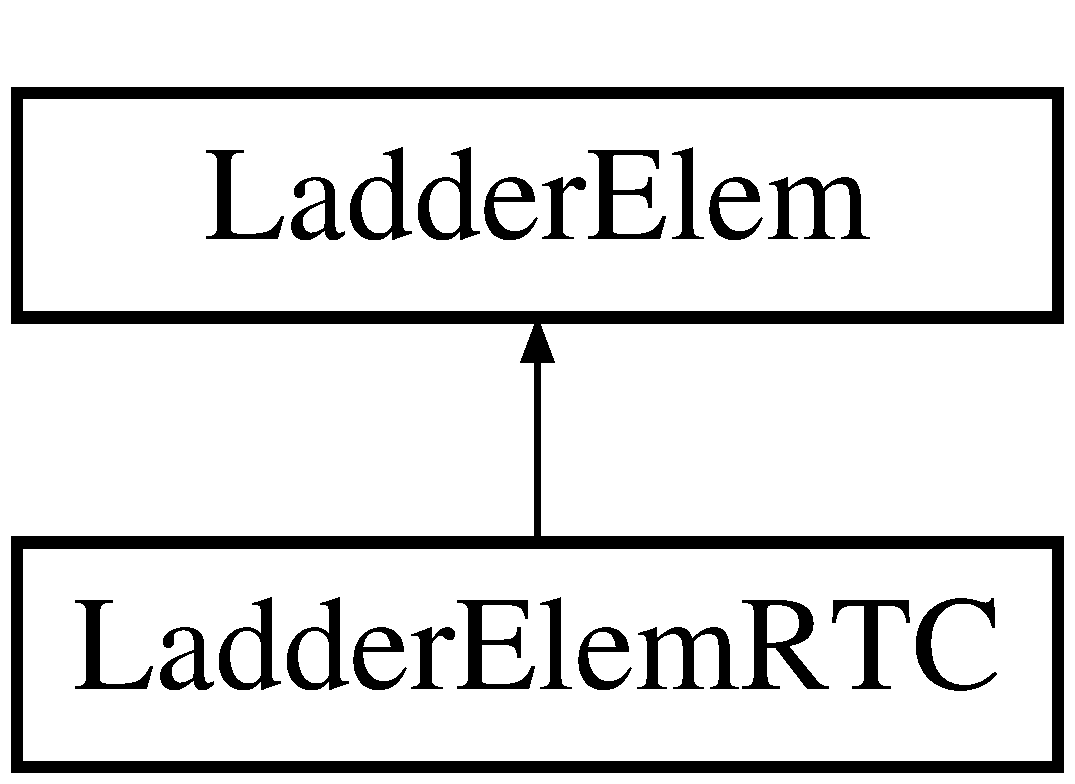
\includegraphics[height=2.000000cm]{class_ladder_elem_r_t_c}
\end{center}
\end{figure}
\subsection*{Public Member Functions}
\begin{DoxyCompactItemize}
\item 
\hypertarget{class_ladder_elem_r_t_c_aa2241d9e92cf019978230d3562c7bf59}{{\bfseries Ladder\-Elem\-R\-T\-C} (\hyperlink{class_ladder_diagram}{Ladder\-Diagram} $\ast$diagram)}\label{class_ladder_elem_r_t_c_aa2241d9e92cf019978230d3562c7bf59}

\item 
\hypertarget{class_ladder_elem_r_t_c_a174dd1bbf4ae1a9054ea2ca5b79221ab}{pair$<$ string, string $>$ {\bfseries Draw\-T\-X\-T} (void)}\label{class_ladder_elem_r_t_c_a174dd1bbf4ae1a9054ea2ca5b79221ab}

\item 
\hypertarget{class_ladder_elem_r_t_c_a5cedf46d6d46899a56e274ded7b70960}{bool {\bfseries Draw\-G\-U\-I} (bool powered\-Before, void $\ast$data)}\label{class_ladder_elem_r_t_c_a5cedf46d6d46899a56e274ded7b70960}

\item 
\hypertarget{class_ladder_elem_r_t_c_a258bcbe40eac5745b5db074d0db60e81}{bool {\bfseries Show\-Dialog} (\hyperlink{struct_ladder_context}{Ladder\-Context} context)}\label{class_ladder_elem_r_t_c_a258bcbe40eac5745b5db074d0db60e81}

\item 
\hypertarget{class_ladder_elem_r_t_c_ad455022d01e9aa861c88e6fa6ccef4d0}{bool {\bfseries internal\-Generate\-Int\-Code} (\hyperlink{class_int_code}{Int\-Code} \&ic)}\label{class_ladder_elem_r_t_c_ad455022d01e9aa861c88e6fa6ccef4d0}

\item 
\hypertarget{class_ladder_elem_r_t_c_a1f547797ab7a0319f43d84657007f402}{void $\ast$ {\bfseries get\-Properties} (void)}\label{class_ladder_elem_r_t_c_a1f547797ab7a0319f43d84657007f402}

\item 
\hypertarget{class_ladder_elem_r_t_c_aa7bdcbbb9da5a8de9017b73efb522066}{bool {\bfseries Can\-Insert} (\hyperlink{struct_ladder_context}{Ladder\-Context} context)}\label{class_ladder_elem_r_t_c_aa7bdcbbb9da5a8de9017b73efb522066}

\item 
\hypertarget{class_ladder_elem_r_t_c_ac32477f5b6782bd58076464ecc6dda1f}{void {\bfseries do\-Post\-Insert} (void)}\label{class_ladder_elem_r_t_c_ac32477f5b6782bd58076464ecc6dda1f}

\item 
\hypertarget{class_ladder_elem_r_t_c_a0d9800d9aaaff110e837812fdad28ca0}{void {\bfseries do\-Post\-Remove} (void)}\label{class_ladder_elem_r_t_c_a0d9800d9aaaff110e837812fdad28ca0}

\item 
\hypertarget{class_ladder_elem_r_t_c_a30a20d9cb39d95e13aa846b1d67437b6}{int {\bfseries get\-Width\-T\-X\-T} (void)}\label{class_ladder_elem_r_t_c_a30a20d9cb39d95e13aa846b1d67437b6}

\item 
\hypertarget{class_ladder_elem_r_t_c_a6ae2125d34a3672a5aee5b446a245d51}{\hyperlink{class_ladder_elem}{Ladder\-Elem} $\ast$ {\bfseries Clone} (\hyperlink{class_ladder_diagram}{Ladder\-Diagram} $\ast$diagram)}\label{class_ladder_elem_r_t_c_a6ae2125d34a3672a5aee5b446a245d51}

\item 
\hypertarget{class_ladder_elem_r_t_c_a2622afd2e2fdf4e1a696f3381f657269}{bool {\bfseries accept\-I\-O} (unsigned long id, e\-Type type)}\label{class_ladder_elem_r_t_c_a2622afd2e2fdf4e1a696f3381f657269}

\item 
\hypertarget{class_ladder_elem_r_t_c_a1dbdd9f38e15b22028f472fb177ec63a}{void {\bfseries update\-I\-O} (\hyperlink{class_ladder_diagram}{Ladder\-Diagram} $\ast$owner, bool is\-Discard)}\label{class_ladder_elem_r_t_c_a1dbdd9f38e15b22028f472fb177ec63a}

\item 
\hypertarget{class_ladder_elem_r_t_c_ac7f02365fb1f79066361fc17d6ecfdec}{e\-Type {\bfseries get\-Allowed\-Type\-I\-O} (unsigned long id)}\label{class_ladder_elem_r_t_c_ac7f02365fb1f79066361fc17d6ecfdec}

\item 
\hypertarget{class_ladder_elem_r_t_c_a3e9fbdc4b2a16a5858ccb67f3136e9a2}{int {\bfseries Search\-And\-Replace} (unsigned long id\-Search, string s\-New\-Text, bool is\-Replace)}\label{class_ladder_elem_r_t_c_a3e9fbdc4b2a16a5858ccb67f3136e9a2}

\item 
\hypertarget{class_ladder_elem_r_t_c_a11fc72a1e141dfd126686b09c468c4a4}{bool {\bfseries internal\-Do\-Undo\-Redo} (bool Is\-Undo, bool is\-Discard, \hyperlink{struct_undo_redo_action}{Undo\-Redo\-Action} \&action)}\label{class_ladder_elem_r_t_c_a11fc72a1e141dfd126686b09c468c4a4}

\end{DoxyCompactItemize}
\subsection*{Additional Inherited Members}


The documentation for this class was generated from the following files\-:\begin{DoxyCompactItemize}
\item 
F\-:/\-S\-V\-N/\-P\-O\-P\-Tools/Ladder\-Objects.\-h\item 
F\-:/\-S\-V\-N/\-P\-O\-P\-Tools/Ladder\-G\-U\-I.\-cpp\item 
F\-:/\-S\-V\-N/\-P\-O\-P\-Tools/Ladder\-Objects.\-cpp\end{DoxyCompactItemize}

\hypertarget{struct_ladder_elem_r_t_c_prop}{\section{Ladder\-Elem\-R\-T\-C\-Prop Struct Reference}
\label{struct_ladder_elem_r_t_c_prop}\index{Ladder\-Elem\-R\-T\-C\-Prop@{Ladder\-Elem\-R\-T\-C\-Prop}}
}
\subsection*{Public Attributes}
\begin{DoxyCompactItemize}
\item 
\hypertarget{struct_ladder_elem_r_t_c_prop_a971c22761bec231e9ddb4807a0b691be}{int {\bfseries mode}}\label{struct_ladder_elem_r_t_c_prop_a971c22761bec231e9ddb4807a0b691be}

\item 
\hypertarget{struct_ladder_elem_r_t_c_prop_a332dfcdec68fee5d34a8970197f24fb4}{unsigned char {\bfseries wday}}\label{struct_ladder_elem_r_t_c_prop_a332dfcdec68fee5d34a8970197f24fb4}

\item 
\hypertarget{struct_ladder_elem_r_t_c_prop_a3fe9a0751cdc950135e2f486c89f801e}{struct tm {\bfseries start}}\label{struct_ladder_elem_r_t_c_prop_a3fe9a0751cdc950135e2f486c89f801e}

\item 
\hypertarget{struct_ladder_elem_r_t_c_prop_a4e2d4d4218a517b6400ea2e38fe174e7}{struct tm {\bfseries end}}\label{struct_ladder_elem_r_t_c_prop_a4e2d4d4218a517b6400ea2e38fe174e7}

\end{DoxyCompactItemize}


The documentation for this struct was generated from the following file\-:\begin{DoxyCompactItemize}
\item 
F\-:/\-S\-V\-N/\-P\-O\-P\-Tools/Ladder\-Objects.\-h\end{DoxyCompactItemize}

\hypertarget{class_ladder_elem_set_bit}{\section{Ladder\-Elem\-Set\-Bit Class Reference}
\label{class_ladder_elem_set_bit}\index{Ladder\-Elem\-Set\-Bit@{Ladder\-Elem\-Set\-Bit}}
}
Inheritance diagram for Ladder\-Elem\-Set\-Bit\-:\begin{figure}[H]
\begin{center}
\leavevmode
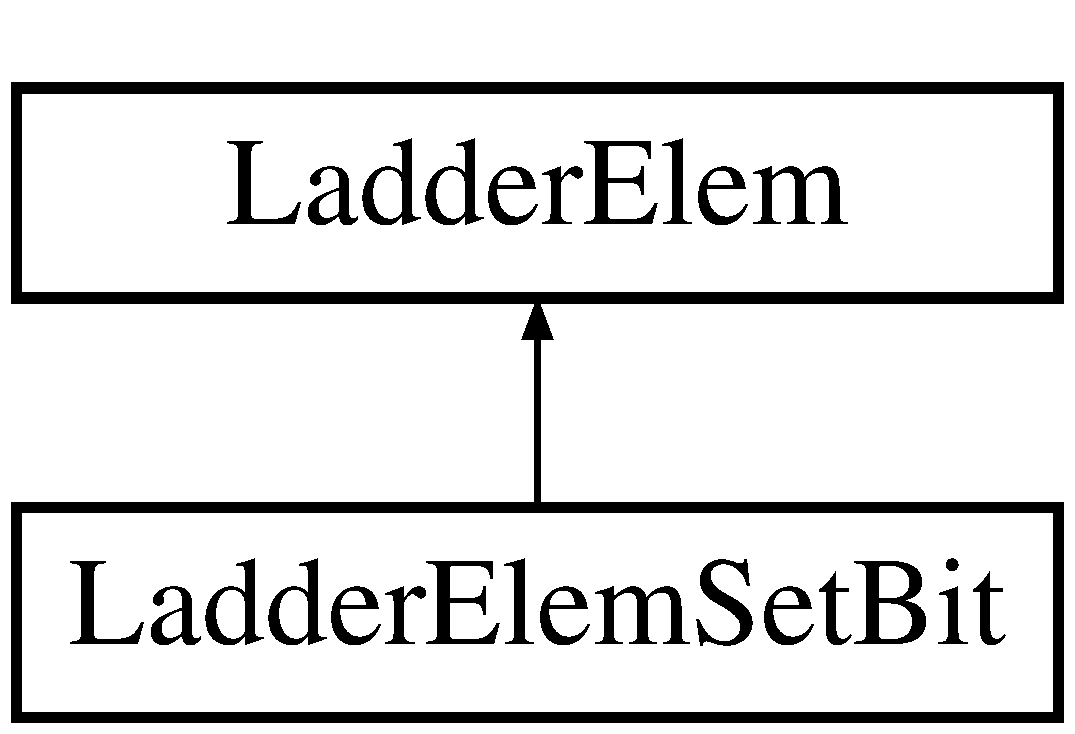
\includegraphics[height=2.000000cm]{class_ladder_elem_set_bit}
\end{center}
\end{figure}
\subsection*{Public Member Functions}
\begin{DoxyCompactItemize}
\item 
\hypertarget{class_ladder_elem_set_bit_abd394b351d25acbbcf24d87b7fe64ea6}{{\bfseries Ladder\-Elem\-Set\-Bit} (\hyperlink{class_ladder_diagram}{Ladder\-Diagram} $\ast$diagram)}\label{class_ladder_elem_set_bit_abd394b351d25acbbcf24d87b7fe64ea6}

\item 
\hypertarget{class_ladder_elem_set_bit_a223b235a409fe56eb633a678d322c9dd}{pair$<$ string, string $>$ {\bfseries Draw\-T\-X\-T} (void)}\label{class_ladder_elem_set_bit_a223b235a409fe56eb633a678d322c9dd}

\item 
\hypertarget{class_ladder_elem_set_bit_a5910294bfeff7af1066c5acd4bf3b809}{bool {\bfseries Draw\-G\-U\-I} (bool powered\-Before, void $\ast$data)}\label{class_ladder_elem_set_bit_a5910294bfeff7af1066c5acd4bf3b809}

\item 
\hypertarget{class_ladder_elem_set_bit_abe91e2b71e4c7c4215d0f3504ec6b98c}{bool {\bfseries Show\-Dialog} (\hyperlink{struct_ladder_context}{Ladder\-Context} context)}\label{class_ladder_elem_set_bit_abe91e2b71e4c7c4215d0f3504ec6b98c}

\item 
\hypertarget{class_ladder_elem_set_bit_a57445938db5175af04230b363c6f7511}{bool {\bfseries internal\-Generate\-Int\-Code} (\hyperlink{class_int_code}{Int\-Code} \&ic)}\label{class_ladder_elem_set_bit_a57445938db5175af04230b363c6f7511}

\item 
\hypertarget{class_ladder_elem_set_bit_a64d64a13c0aaf8157c6d4e64e88e8f33}{void $\ast$ {\bfseries get\-Properties} (void)}\label{class_ladder_elem_set_bit_a64d64a13c0aaf8157c6d4e64e88e8f33}

\item 
\hypertarget{class_ladder_elem_set_bit_ae6353b6f2abcf1065f821fb24cc6c48a}{bool {\bfseries Can\-Insert} (\hyperlink{struct_ladder_context}{Ladder\-Context} context)}\label{class_ladder_elem_set_bit_ae6353b6f2abcf1065f821fb24cc6c48a}

\item 
\hypertarget{class_ladder_elem_set_bit_a05f83b6188d8b3a94dba591735218dc9}{void {\bfseries do\-Post\-Insert} (void)}\label{class_ladder_elem_set_bit_a05f83b6188d8b3a94dba591735218dc9}

\item 
\hypertarget{class_ladder_elem_set_bit_a1e8d39108ecb7768724eebbab2ef57a8}{void {\bfseries do\-Post\-Remove} (void)}\label{class_ladder_elem_set_bit_a1e8d39108ecb7768724eebbab2ef57a8}

\item 
\hypertarget{class_ladder_elem_set_bit_a7d3a4c99c7902c09403dfd1c428f539c}{int {\bfseries get\-Width\-T\-X\-T} (void)}\label{class_ladder_elem_set_bit_a7d3a4c99c7902c09403dfd1c428f539c}

\item 
\hypertarget{class_ladder_elem_set_bit_a0ce5b27f59bb09ab516d9b1edd9d1d10}{\hyperlink{class_ladder_elem}{Ladder\-Elem} $\ast$ {\bfseries Clone} (\hyperlink{class_ladder_diagram}{Ladder\-Diagram} $\ast$diagram)}\label{class_ladder_elem_set_bit_a0ce5b27f59bb09ab516d9b1edd9d1d10}

\item 
\hypertarget{class_ladder_elem_set_bit_ab1ee8f8328861e134ce06aa904b4c720}{bool {\bfseries accept\-I\-O} (unsigned long id, e\-Type type)}\label{class_ladder_elem_set_bit_ab1ee8f8328861e134ce06aa904b4c720}

\item 
\hypertarget{class_ladder_elem_set_bit_ac8ad1a02c4e5e90fa1abe80bc2e3eae8}{void {\bfseries update\-I\-O} (\hyperlink{class_ladder_diagram}{Ladder\-Diagram} $\ast$owner, bool is\-Discard)}\label{class_ladder_elem_set_bit_ac8ad1a02c4e5e90fa1abe80bc2e3eae8}

\item 
\hypertarget{class_ladder_elem_set_bit_ac09a788b63d2d706708a8d6bf1effcb6}{e\-Type {\bfseries get\-Allowed\-Type\-I\-O} (unsigned long id)}\label{class_ladder_elem_set_bit_ac09a788b63d2d706708a8d6bf1effcb6}

\item 
\hypertarget{class_ladder_elem_set_bit_a5d6d0e5a4857f6b60843df96909f9ec8}{int {\bfseries Search\-And\-Replace} (unsigned long id\-Search, string s\-New\-Text, bool is\-Replace)}\label{class_ladder_elem_set_bit_a5d6d0e5a4857f6b60843df96909f9ec8}

\item 
\hypertarget{class_ladder_elem_set_bit_ad51903217bd241cf7994744b295c4221}{bool {\bfseries internal\-Do\-Undo\-Redo} (bool Is\-Undo, bool is\-Discard, \hyperlink{struct_undo_redo_action}{Undo\-Redo\-Action} \&action)}\label{class_ladder_elem_set_bit_ad51903217bd241cf7994744b295c4221}

\end{DoxyCompactItemize}
\subsection*{Additional Inherited Members}


The documentation for this class was generated from the following files\-:\begin{DoxyCompactItemize}
\item 
F\-:/\-S\-V\-N/\-P\-O\-P\-Tools/Ladder\-Objects.\-h\item 
F\-:/\-S\-V\-N/\-P\-O\-P\-Tools/Ladder\-G\-U\-I.\-cpp\item 
F\-:/\-S\-V\-N/\-P\-O\-P\-Tools/Ladder\-Objects.\-cpp\end{DoxyCompactItemize}

\hypertarget{struct_ladder_elem_set_bit_prop}{\section{Ladder\-Elem\-Set\-Bit\-Prop Struct Reference}
\label{struct_ladder_elem_set_bit_prop}\index{Ladder\-Elem\-Set\-Bit\-Prop@{Ladder\-Elem\-Set\-Bit\-Prop}}
}
\subsection*{Public Attributes}
\begin{DoxyCompactItemize}
\item 
\hypertarget{struct_ladder_elem_set_bit_prop_a96851f82bdbd10e0b4589229ddd93ea2}{pair$<$ unsigned long, int $>$ {\bfseries id\-Name}}\label{struct_ladder_elem_set_bit_prop_a96851f82bdbd10e0b4589229ddd93ea2}

\item 
\hypertarget{struct_ladder_elem_set_bit_prop_abde23362872741a5565a4aa36fbe1a52}{int {\bfseries bit}}\label{struct_ladder_elem_set_bit_prop_abde23362872741a5565a4aa36fbe1a52}

\item 
\hypertarget{struct_ladder_elem_set_bit_prop_a61189db763c9eae18ace42a69529887e}{bool {\bfseries set}}\label{struct_ladder_elem_set_bit_prop_a61189db763c9eae18ace42a69529887e}

\end{DoxyCompactItemize}


The documentation for this struct was generated from the following file\-:\begin{DoxyCompactItemize}
\item 
F\-:/\-S\-V\-N/\-P\-O\-P\-Tools/Ladder\-Objects.\-h\end{DoxyCompactItemize}

\hypertarget{class_ladder_elem_set_da}{\section{Ladder\-Elem\-Set\-Da Class Reference}
\label{class_ladder_elem_set_da}\index{Ladder\-Elem\-Set\-Da@{Ladder\-Elem\-Set\-Da}}
}
Inheritance diagram for Ladder\-Elem\-Set\-Da\-:\begin{figure}[H]
\begin{center}
\leavevmode
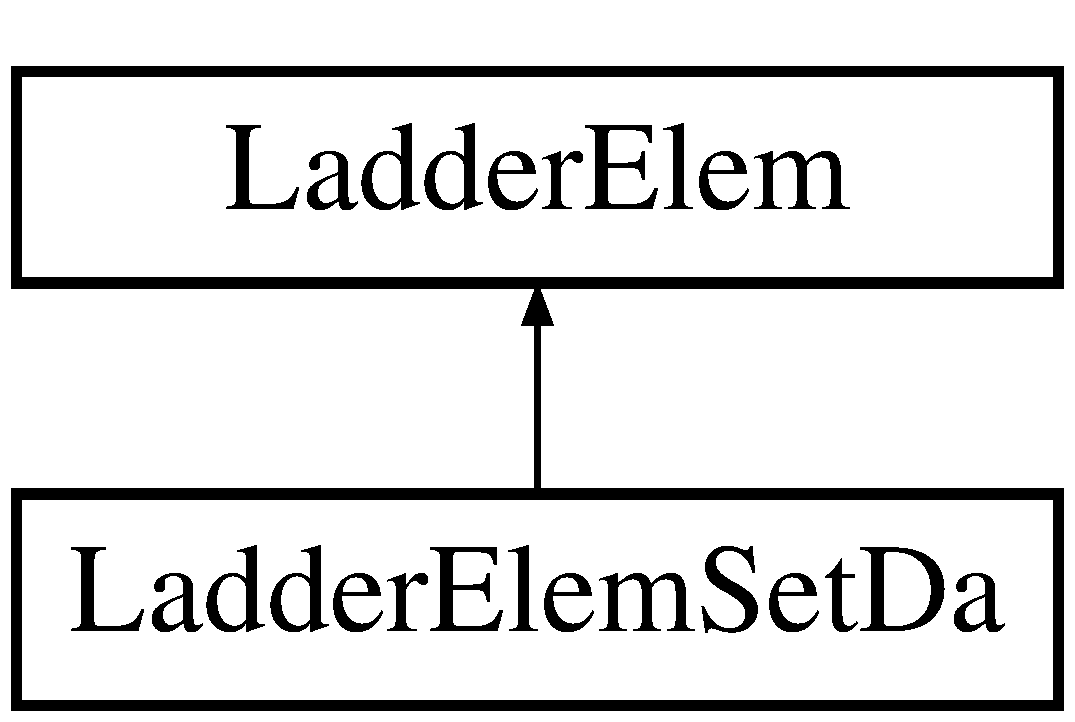
\includegraphics[height=2.000000cm]{class_ladder_elem_set_da}
\end{center}
\end{figure}
\subsection*{Public Member Functions}
\begin{DoxyCompactItemize}
\item 
\hypertarget{class_ladder_elem_set_da_a11f09cb31790b7701d06d355874913cb}{{\bfseries Ladder\-Elem\-Set\-Da} (\hyperlink{class_ladder_diagram}{Ladder\-Diagram} $\ast$diagram)}\label{class_ladder_elem_set_da_a11f09cb31790b7701d06d355874913cb}

\item 
\hypertarget{class_ladder_elem_set_da_a464038a097363a7c8b990155c1557dfd}{pair$<$ string, string $>$ {\bfseries Draw\-T\-X\-T} (void)}\label{class_ladder_elem_set_da_a464038a097363a7c8b990155c1557dfd}

\item 
\hypertarget{class_ladder_elem_set_da_a5484cb40622e3406243fac5e19a2f5b6}{bool {\bfseries Draw\-G\-U\-I} (bool powered\-Before, void $\ast$data)}\label{class_ladder_elem_set_da_a5484cb40622e3406243fac5e19a2f5b6}

\item 
\hypertarget{class_ladder_elem_set_da_acf9653c802b9c67827d68df188bcb752}{bool {\bfseries Show\-Dialog} (\hyperlink{struct_ladder_context}{Ladder\-Context} context)}\label{class_ladder_elem_set_da_acf9653c802b9c67827d68df188bcb752}

\item 
\hypertarget{class_ladder_elem_set_da_ae67decbd2195a52b15f4201619e13085}{bool {\bfseries internal\-Generate\-Int\-Code} (\hyperlink{class_int_code}{Int\-Code} \&ic)}\label{class_ladder_elem_set_da_ae67decbd2195a52b15f4201619e13085}

\item 
\hypertarget{class_ladder_elem_set_da_a449fb4013e8631ce1661062e9c6cb842}{void $\ast$ {\bfseries get\-Properties} (void)}\label{class_ladder_elem_set_da_a449fb4013e8631ce1661062e9c6cb842}

\item 
\hypertarget{class_ladder_elem_set_da_a28980478d54de2547759ab45f112875e}{bool {\bfseries Can\-Insert} (\hyperlink{struct_ladder_context}{Ladder\-Context} context)}\label{class_ladder_elem_set_da_a28980478d54de2547759ab45f112875e}

\item 
\hypertarget{class_ladder_elem_set_da_abb2580f9ed193439125659d806cde746}{bool {\bfseries is\-Valid\-Da\-Value} (string new\-\_\-name, int new\-\_\-mode)}\label{class_ladder_elem_set_da_abb2580f9ed193439125659d806cde746}

\item 
\hypertarget{class_ladder_elem_set_da_a2cdac2b0eae66943a4f181cdfd1d071e}{void {\bfseries do\-Post\-Insert} (void)}\label{class_ladder_elem_set_da_a2cdac2b0eae66943a4f181cdfd1d071e}

\item 
\hypertarget{class_ladder_elem_set_da_a92a670e2f63296a68850d4c45e96f3f2}{void {\bfseries do\-Post\-Remove} (void)}\label{class_ladder_elem_set_da_a92a670e2f63296a68850d4c45e96f3f2}

\item 
\hypertarget{class_ladder_elem_set_da_a8df70b781e022743051292f1473512fa}{int {\bfseries get\-Width\-T\-X\-T} (void)}\label{class_ladder_elem_set_da_a8df70b781e022743051292f1473512fa}

\item 
\hypertarget{class_ladder_elem_set_da_ace8c2b2a872c0ee9c5ec73e04ebcd087}{\hyperlink{class_ladder_elem}{Ladder\-Elem} $\ast$ {\bfseries Clone} (\hyperlink{class_ladder_diagram}{Ladder\-Diagram} $\ast$diagram)}\label{class_ladder_elem_set_da_ace8c2b2a872c0ee9c5ec73e04ebcd087}

\item 
\hypertarget{class_ladder_elem_set_da_ad97a6da4076ce9bad529bd7eb960ba61}{bool {\bfseries accept\-I\-O} (unsigned long id, e\-Type type)}\label{class_ladder_elem_set_da_ad97a6da4076ce9bad529bd7eb960ba61}

\item 
\hypertarget{class_ladder_elem_set_da_a71306b851d353221010ea4bb6fe7e828}{void {\bfseries update\-I\-O} (\hyperlink{class_ladder_diagram}{Ladder\-Diagram} $\ast$owner, bool is\-Discard)}\label{class_ladder_elem_set_da_a71306b851d353221010ea4bb6fe7e828}

\item 
\hypertarget{class_ladder_elem_set_da_a9f6cd89915e89478dbe5fcf3da993866}{e\-Type {\bfseries get\-Allowed\-Type\-I\-O} (unsigned long id)}\label{class_ladder_elem_set_da_a9f6cd89915e89478dbe5fcf3da993866}

\item 
\hypertarget{class_ladder_elem_set_da_a801b357fe0ac15b63671520713f2ff66}{int {\bfseries Search\-And\-Replace} (unsigned long id\-Search, string s\-New\-Text, bool is\-Replace)}\label{class_ladder_elem_set_da_a801b357fe0ac15b63671520713f2ff66}

\item 
\hypertarget{class_ladder_elem_set_da_ad6b3a0c03aee6306d58962c0626162e1}{bool {\bfseries internal\-Do\-Undo\-Redo} (bool Is\-Undo, bool is\-Discard, \hyperlink{struct_undo_redo_action}{Undo\-Redo\-Action} \&action)}\label{class_ladder_elem_set_da_ad6b3a0c03aee6306d58962c0626162e1}

\end{DoxyCompactItemize}
\subsection*{Additional Inherited Members}


The documentation for this class was generated from the following files\-:\begin{DoxyCompactItemize}
\item 
F\-:/\-S\-V\-N/\-P\-O\-P\-Tools/Ladder\-Objects.\-h\item 
F\-:/\-S\-V\-N/\-P\-O\-P\-Tools/Ladder\-G\-U\-I.\-cpp\item 
F\-:/\-S\-V\-N/\-P\-O\-P\-Tools/Ladder\-Objects.\-cpp\end{DoxyCompactItemize}

\hypertarget{struct_ladder_elem_set_da_prop}{\section{Ladder\-Elem\-Set\-Da\-Prop Struct Reference}
\label{struct_ladder_elem_set_da_prop}\index{Ladder\-Elem\-Set\-Da\-Prop@{Ladder\-Elem\-Set\-Da\-Prop}}
}
\subsection*{Public Attributes}
\begin{DoxyCompactItemize}
\item 
\hypertarget{struct_ladder_elem_set_da_prop_a64d4a03956a85ad1f0d598853ac38fda}{pair$<$ unsigned long, int $>$ {\bfseries id\-Name}}\label{struct_ladder_elem_set_da_prop_a64d4a03956a85ad1f0d598853ac38fda}

\item 
\hypertarget{struct_ladder_elem_set_da_prop_ab4bae96f58807332b82933a8240563b9}{int {\bfseries mode}}\label{struct_ladder_elem_set_da_prop_ab4bae96f58807332b82933a8240563b9}

\end{DoxyCompactItemize}


The documentation for this struct was generated from the following file\-:\begin{DoxyCompactItemize}
\item 
F\-:/\-S\-V\-N/\-P\-O\-P\-Tools/Ladder\-Objects.\-h\end{DoxyCompactItemize}

\hypertarget{class_ladder_elem_set_p_w_m}{\section{Ladder\-Elem\-Set\-P\-W\-M Class Reference}
\label{class_ladder_elem_set_p_w_m}\index{Ladder\-Elem\-Set\-P\-W\-M@{Ladder\-Elem\-Set\-P\-W\-M}}
}
Inheritance diagram for Ladder\-Elem\-Set\-P\-W\-M\-:\begin{figure}[H]
\begin{center}
\leavevmode
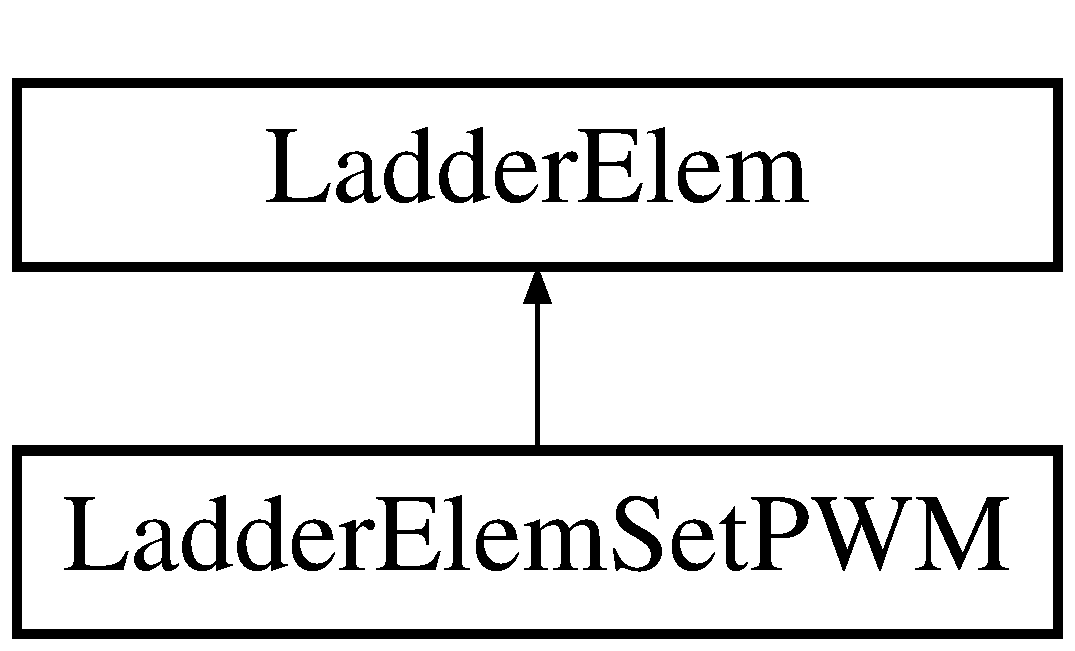
\includegraphics[height=2.000000cm]{class_ladder_elem_set_p_w_m}
\end{center}
\end{figure}
\subsection*{Public Member Functions}
\begin{DoxyCompactItemize}
\item 
\hypertarget{class_ladder_elem_set_p_w_m_a24dfc2064f6165210d4844b382ebe51a}{{\bfseries Ladder\-Elem\-Set\-P\-W\-M} (\hyperlink{class_ladder_diagram}{Ladder\-Diagram} $\ast$diagram)}\label{class_ladder_elem_set_p_w_m_a24dfc2064f6165210d4844b382ebe51a}

\item 
\hypertarget{class_ladder_elem_set_p_w_m_af6c4eb679608df546936b44cebc16a8b}{pair$<$ string, string $>$ {\bfseries Draw\-T\-X\-T} (void)}\label{class_ladder_elem_set_p_w_m_af6c4eb679608df546936b44cebc16a8b}

\item 
\hypertarget{class_ladder_elem_set_p_w_m_aaaf95c1e471cd91e63dfb0e94d5f89d2}{bool {\bfseries Draw\-G\-U\-I} (bool powered\-Before, void $\ast$data)}\label{class_ladder_elem_set_p_w_m_aaaf95c1e471cd91e63dfb0e94d5f89d2}

\item 
\hypertarget{class_ladder_elem_set_p_w_m_a069fc8ba1eec27d5fabb6b75b181aa2e}{bool {\bfseries Show\-Dialog} (\hyperlink{struct_ladder_context}{Ladder\-Context} context)}\label{class_ladder_elem_set_p_w_m_a069fc8ba1eec27d5fabb6b75b181aa2e}

\item 
\hypertarget{class_ladder_elem_set_p_w_m_a981d9f5a070bf989c897d7cd8c9be171}{bool {\bfseries internal\-Generate\-Int\-Code} (\hyperlink{class_int_code}{Int\-Code} \&ic)}\label{class_ladder_elem_set_p_w_m_a981d9f5a070bf989c897d7cd8c9be171}

\item 
\hypertarget{class_ladder_elem_set_p_w_m_a1b753dca949fc99e004c236d937e4973}{bool {\bfseries Can\-Insert} (\hyperlink{struct_ladder_context}{Ladder\-Context} context)}\label{class_ladder_elem_set_p_w_m_a1b753dca949fc99e004c236d937e4973}

\item 
\hypertarget{class_ladder_elem_set_p_w_m_ac0f34dd302aebb93c0a631758d3642aa}{void {\bfseries do\-Post\-Insert} (void)}\label{class_ladder_elem_set_p_w_m_ac0f34dd302aebb93c0a631758d3642aa}

\item 
\hypertarget{class_ladder_elem_set_p_w_m_aa06b6da31442eef38fdd794e0172023b}{void {\bfseries do\-Post\-Remove} (void)}\label{class_ladder_elem_set_p_w_m_aa06b6da31442eef38fdd794e0172023b}

\item 
\hypertarget{class_ladder_elem_set_p_w_m_a14bd0381707847f3dcce8b7aefae72d6}{void $\ast$ {\bfseries get\-Properties} (void)}\label{class_ladder_elem_set_p_w_m_a14bd0381707847f3dcce8b7aefae72d6}

\item 
\hypertarget{class_ladder_elem_set_p_w_m_a7ff1e95ce7fffc10cf635fef5767954c}{int {\bfseries get\-Width\-T\-X\-T} (void)}\label{class_ladder_elem_set_p_w_m_a7ff1e95ce7fffc10cf635fef5767954c}

\item 
\hypertarget{class_ladder_elem_set_p_w_m_a07ce2f8eb4baefb5115ee4d60d8cbfaa}{\hyperlink{class_ladder_elem}{Ladder\-Elem} $\ast$ {\bfseries Clone} (\hyperlink{class_ladder_diagram}{Ladder\-Diagram} $\ast$diagram)}\label{class_ladder_elem_set_p_w_m_a07ce2f8eb4baefb5115ee4d60d8cbfaa}

\item 
\hypertarget{class_ladder_elem_set_p_w_m_abd0b71e930162e0a1b784ee3fd37b25f}{bool {\bfseries accept\-I\-O} (unsigned long id, e\-Type type)}\label{class_ladder_elem_set_p_w_m_abd0b71e930162e0a1b784ee3fd37b25f}

\item 
\hypertarget{class_ladder_elem_set_p_w_m_a43ab15cded07eeeb4418324ca4211470}{void {\bfseries update\-I\-O} (\hyperlink{class_ladder_diagram}{Ladder\-Diagram} $\ast$owner, bool is\-Discard)}\label{class_ladder_elem_set_p_w_m_a43ab15cded07eeeb4418324ca4211470}

\item 
\hypertarget{class_ladder_elem_set_p_w_m_a8d9670c478ce8f6c2eb6c4924bc79b00}{e\-Type {\bfseries get\-Allowed\-Type\-I\-O} (unsigned long id)}\label{class_ladder_elem_set_p_w_m_a8d9670c478ce8f6c2eb6c4924bc79b00}

\item 
\hypertarget{class_ladder_elem_set_p_w_m_ab51f897c023d60ed93c731c68e009fed}{int {\bfseries Search\-And\-Replace} (unsigned long id\-Search, string s\-New\-Text, bool is\-Replace)}\label{class_ladder_elem_set_p_w_m_ab51f897c023d60ed93c731c68e009fed}

\item 
\hypertarget{class_ladder_elem_set_p_w_m_a31fa8321cf9dfad700d03b3a7671ae8d}{bool {\bfseries internal\-Do\-Undo\-Redo} (bool Is\-Undo, bool is\-Discard, \hyperlink{struct_undo_redo_action}{Undo\-Redo\-Action} \&action)}\label{class_ladder_elem_set_p_w_m_a31fa8321cf9dfad700d03b3a7671ae8d}

\end{DoxyCompactItemize}
\subsection*{Additional Inherited Members}


The documentation for this class was generated from the following files\-:\begin{DoxyCompactItemize}
\item 
F\-:/\-S\-V\-N/\-P\-O\-P\-Tools/Ladder\-Objects.\-h\item 
F\-:/\-S\-V\-N/\-P\-O\-P\-Tools/Ladder\-G\-U\-I.\-cpp\item 
F\-:/\-S\-V\-N/\-P\-O\-P\-Tools/Ladder\-Objects.\-cpp\end{DoxyCompactItemize}

\hypertarget{struct_ladder_elem_set_p_w_m_prop}{\section{Ladder\-Elem\-Set\-P\-W\-M\-Prop Struct Reference}
\label{struct_ladder_elem_set_p_w_m_prop}\index{Ladder\-Elem\-Set\-P\-W\-M\-Prop@{Ladder\-Elem\-Set\-P\-W\-M\-Prop}}
}
\subsection*{Public Attributes}
\begin{DoxyCompactItemize}
\item 
\hypertarget{struct_ladder_elem_set_p_w_m_prop_a1c55f95240f3796813aad1c55c273b40}{pair$<$ unsigned long, int $>$ {\bfseries id\-Name}}\label{struct_ladder_elem_set_p_w_m_prop_a1c55f95240f3796813aad1c55c273b40}

\item 
\hypertarget{struct_ladder_elem_set_p_w_m_prop_a4a16481699c58bef0a0a2db1a614eed4}{int {\bfseries target\-Freq}}\label{struct_ladder_elem_set_p_w_m_prop_a4a16481699c58bef0a0a2db1a614eed4}

\end{DoxyCompactItemize}


The documentation for this struct was generated from the following file\-:\begin{DoxyCompactItemize}
\item 
F\-:/\-S\-V\-N/\-P\-O\-P\-Tools/Ladder\-Objects.\-h\end{DoxyCompactItemize}

\hypertarget{class_ladder_elem_shift_register}{\section{Ladder\-Elem\-Shift\-Register Class Reference}
\label{class_ladder_elem_shift_register}\index{Ladder\-Elem\-Shift\-Register@{Ladder\-Elem\-Shift\-Register}}
}
Inheritance diagram for Ladder\-Elem\-Shift\-Register\-:\begin{figure}[H]
\begin{center}
\leavevmode
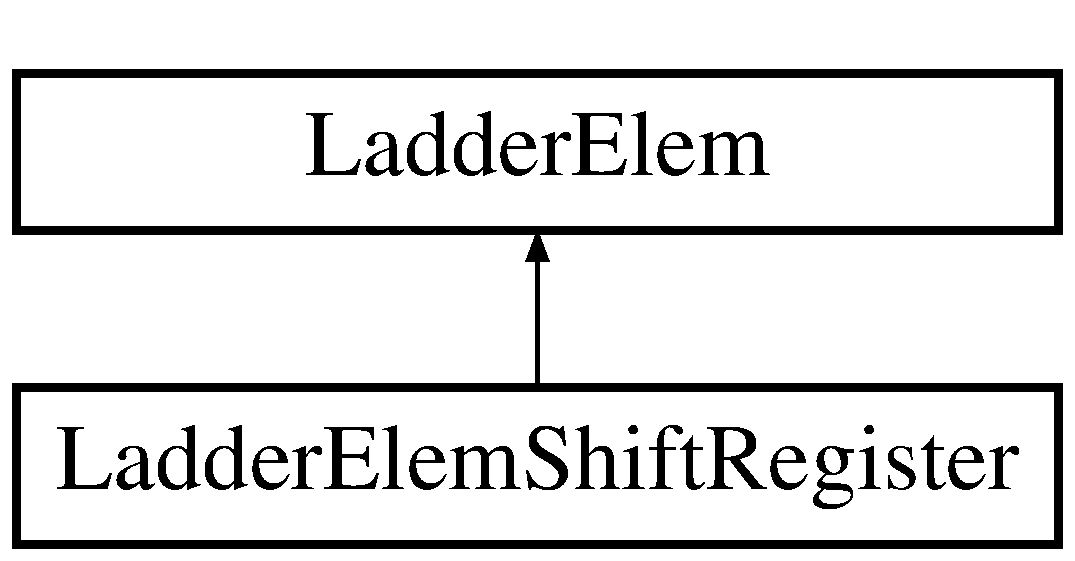
\includegraphics[height=2.000000cm]{class_ladder_elem_shift_register}
\end{center}
\end{figure}
\subsection*{Public Member Functions}
\begin{DoxyCompactItemize}
\item 
\hypertarget{class_ladder_elem_shift_register_a94d17c98d27949b489c48ff8f2a6aec1}{{\bfseries Ladder\-Elem\-Shift\-Register} (\hyperlink{class_ladder_diagram}{Ladder\-Diagram} $\ast$diagram)}\label{class_ladder_elem_shift_register_a94d17c98d27949b489c48ff8f2a6aec1}

\item 
\hypertarget{class_ladder_elem_shift_register_a85d5700e1e12bd11bd20fde7a5d88db9}{pair$<$ string, string $>$ {\bfseries Draw\-T\-X\-T} (void)}\label{class_ladder_elem_shift_register_a85d5700e1e12bd11bd20fde7a5d88db9}

\item 
\hypertarget{class_ladder_elem_shift_register_afd462235842c505e3774b0b0d2e18bf4}{bool {\bfseries Draw\-G\-U\-I} (bool powered\-Before, void $\ast$data)}\label{class_ladder_elem_shift_register_afd462235842c505e3774b0b0d2e18bf4}

\item 
\hypertarget{class_ladder_elem_shift_register_abb5c346b0b86d4343a7aabdb04b45188}{bool {\bfseries Show\-Dialog} (\hyperlink{struct_ladder_context}{Ladder\-Context} context)}\label{class_ladder_elem_shift_register_abb5c346b0b86d4343a7aabdb04b45188}

\item 
\hypertarget{class_ladder_elem_shift_register_ad8fd3dea74677cd663463d615987cd36}{bool {\bfseries internal\-Generate\-Int\-Code} (\hyperlink{class_int_code}{Int\-Code} \&ic)}\label{class_ladder_elem_shift_register_ad8fd3dea74677cd663463d615987cd36}

\item 
\hypertarget{class_ladder_elem_shift_register_ae2bf2f0c7e48fb4123de69ca5ad0b7d0}{void $\ast$ {\bfseries get\-Properties} (void)}\label{class_ladder_elem_shift_register_ae2bf2f0c7e48fb4123de69ca5ad0b7d0}

\item 
\hypertarget{class_ladder_elem_shift_register_a8756101db0e36d62a689b95b86e0343f}{bool {\bfseries Can\-Insert} (\hyperlink{struct_ladder_context}{Ladder\-Context} context)}\label{class_ladder_elem_shift_register_a8756101db0e36d62a689b95b86e0343f}

\item 
\hypertarget{class_ladder_elem_shift_register_a57ff08ddec87af31ea531fbf42588b3c}{void {\bfseries do\-Post\-Insert} (void)}\label{class_ladder_elem_shift_register_a57ff08ddec87af31ea531fbf42588b3c}

\item 
\hypertarget{class_ladder_elem_shift_register_adcf6dd85ca71d40b96ccdc51afefe2d9}{void {\bfseries do\-Post\-Remove} (void)}\label{class_ladder_elem_shift_register_adcf6dd85ca71d40b96ccdc51afefe2d9}

\item 
\hypertarget{class_ladder_elem_shift_register_a003521734c3c5acf95d58792fe9ef122}{int {\bfseries get\-Width\-T\-X\-T} (void)}\label{class_ladder_elem_shift_register_a003521734c3c5acf95d58792fe9ef122}

\item 
\hypertarget{class_ladder_elem_shift_register_a1e534d468bc1e9f55750124d3dceff6f}{\hyperlink{class_ladder_elem}{Ladder\-Elem} $\ast$ {\bfseries Clone} (\hyperlink{class_ladder_diagram}{Ladder\-Diagram} $\ast$diagram)}\label{class_ladder_elem_shift_register_a1e534d468bc1e9f55750124d3dceff6f}

\item 
\hypertarget{class_ladder_elem_shift_register_aae3943995c00fd7794eeec61739cfee0}{bool {\bfseries accept\-I\-O} (unsigned long id, e\-Type type)}\label{class_ladder_elem_shift_register_aae3943995c00fd7794eeec61739cfee0}

\item 
\hypertarget{class_ladder_elem_shift_register_ab298430c6aa4aecbb58c17011e60b257}{void {\bfseries update\-I\-O} (\hyperlink{class_ladder_diagram}{Ladder\-Diagram} $\ast$owner, bool is\-Discard)}\label{class_ladder_elem_shift_register_ab298430c6aa4aecbb58c17011e60b257}

\item 
\hypertarget{class_ladder_elem_shift_register_ace3bdb8b73c708ef6640d8a56304063a}{e\-Type {\bfseries get\-Allowed\-Type\-I\-O} (unsigned long id)}\label{class_ladder_elem_shift_register_ace3bdb8b73c708ef6640d8a56304063a}

\item 
\hypertarget{class_ladder_elem_shift_register_a685dda3ed459562234c8ee468e478588}{int {\bfseries Search\-And\-Replace} (unsigned long id\-Search, string s\-New\-Text, bool is\-Replace)}\label{class_ladder_elem_shift_register_a685dda3ed459562234c8ee468e478588}

\item 
\hypertarget{class_ladder_elem_shift_register_ac7552aa5978467b72c0ecd90312bccc5}{bool {\bfseries internal\-Do\-Undo\-Redo} (bool Is\-Undo, bool is\-Discard, \hyperlink{struct_undo_redo_action}{Undo\-Redo\-Action} \&action)}\label{class_ladder_elem_shift_register_ac7552aa5978467b72c0ecd90312bccc5}

\end{DoxyCompactItemize}
\subsection*{Additional Inherited Members}


The documentation for this class was generated from the following files\-:\begin{DoxyCompactItemize}
\item 
F\-:/\-S\-V\-N/\-P\-O\-P\-Tools/Ladder\-Objects.\-h\item 
F\-:/\-S\-V\-N/\-P\-O\-P\-Tools/Ladder\-G\-U\-I.\-cpp\item 
F\-:/\-S\-V\-N/\-P\-O\-P\-Tools/Ladder\-Objects.\-cpp\end{DoxyCompactItemize}

\hypertarget{struct_ladder_elem_shift_register_prop}{\section{Ladder\-Elem\-Shift\-Register\-Prop Struct Reference}
\label{struct_ladder_elem_shift_register_prop}\index{Ladder\-Elem\-Shift\-Register\-Prop@{Ladder\-Elem\-Shift\-Register\-Prop}}
}
\subsection*{Public Attributes}
\begin{DoxyCompactItemize}
\item 
\hypertarget{struct_ladder_elem_shift_register_prop_a867554f392d4d9d965e4e23bc2937556}{vector$<$ pair$<$ unsigned long, \\*
int $>$ $>$ {\bfseries vector\-Id\-Regs}}\label{struct_ladder_elem_shift_register_prop_a867554f392d4d9d965e4e23bc2937556}

\item 
\hypertarget{struct_ladder_elem_shift_register_prop_ae870a64e4b53e71363d0f82ae2bb2a7e}{string {\bfseries name\-Reg}}\label{struct_ladder_elem_shift_register_prop_ae870a64e4b53e71363d0f82ae2bb2a7e}

\item 
\hypertarget{struct_ladder_elem_shift_register_prop_aedfdf7a8855b1c540c9f8d8e3e913cc8}{int {\bfseries stages}}\label{struct_ladder_elem_shift_register_prop_aedfdf7a8855b1c540c9f8d8e3e913cc8}

\end{DoxyCompactItemize}


The documentation for this struct was generated from the following file\-:\begin{DoxyCompactItemize}
\item 
F\-:/\-S\-V\-N/\-P\-O\-P\-Tools/Ladder\-Objects.\-h\end{DoxyCompactItemize}

\hypertarget{class_ladder_elem_sqrt}{\section{Ladder\-Elem\-Sqrt Class Reference}
\label{class_ladder_elem_sqrt}\index{Ladder\-Elem\-Sqrt@{Ladder\-Elem\-Sqrt}}
}
Inheritance diagram for Ladder\-Elem\-Sqrt\-:\begin{figure}[H]
\begin{center}
\leavevmode
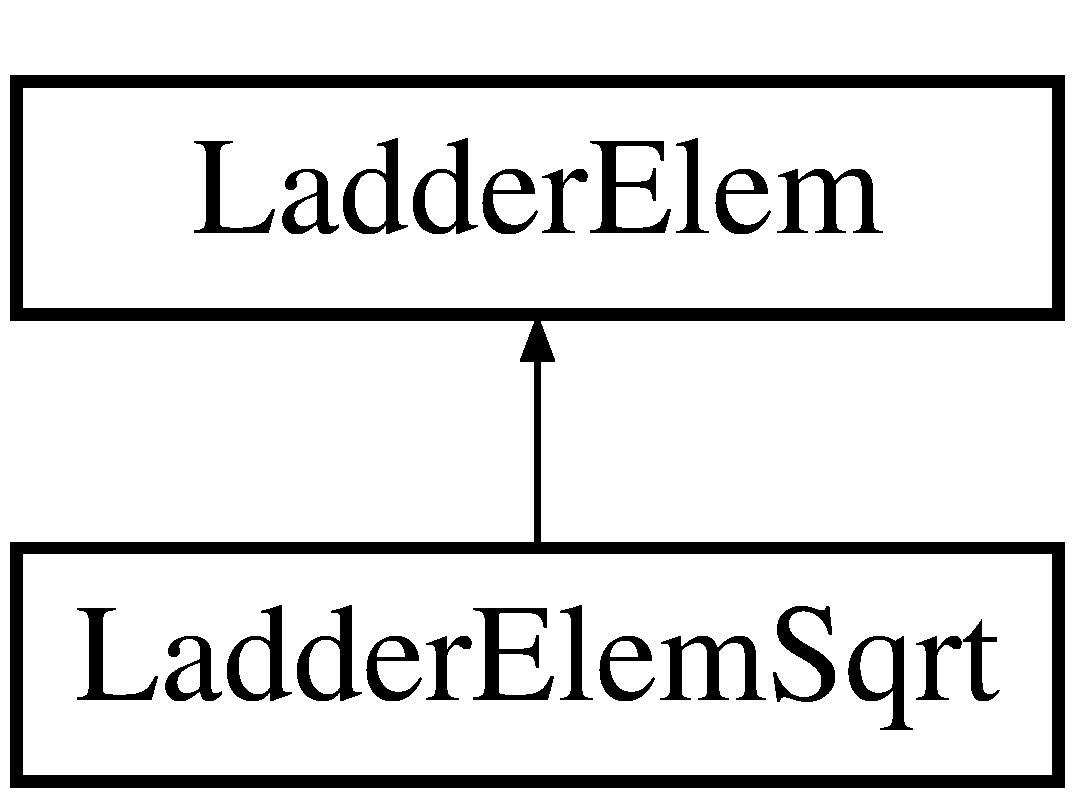
\includegraphics[height=2.000000cm]{class_ladder_elem_sqrt}
\end{center}
\end{figure}
\subsection*{Public Member Functions}
\begin{DoxyCompactItemize}
\item 
\hypertarget{class_ladder_elem_sqrt_a7c795e5b9cf1c464e9e55b4720c2bcb2}{{\bfseries Ladder\-Elem\-Sqrt} (\hyperlink{class_ladder_diagram}{Ladder\-Diagram} $\ast$diagram)}\label{class_ladder_elem_sqrt_a7c795e5b9cf1c464e9e55b4720c2bcb2}

\item 
\hypertarget{class_ladder_elem_sqrt_a0eda4fbdcecf6a1875b12eeb79635202}{pair$<$ string, string $>$ {\bfseries Draw\-T\-X\-T} (void)}\label{class_ladder_elem_sqrt_a0eda4fbdcecf6a1875b12eeb79635202}

\item 
\hypertarget{class_ladder_elem_sqrt_a1e56313b2646e910ba4995c91955a3ed}{bool {\bfseries Draw\-G\-U\-I} (bool powered\-Before, void $\ast$data)}\label{class_ladder_elem_sqrt_a1e56313b2646e910ba4995c91955a3ed}

\item 
\hypertarget{class_ladder_elem_sqrt_a1c3231cd0909b7692d24f03a464940ca}{bool {\bfseries Show\-Dialog} (\hyperlink{struct_ladder_context}{Ladder\-Context} context)}\label{class_ladder_elem_sqrt_a1c3231cd0909b7692d24f03a464940ca}

\item 
\hypertarget{class_ladder_elem_sqrt_ab2fe3efacbd9e98dd046274c651fc904}{bool {\bfseries internal\-Generate\-Int\-Code} (\hyperlink{class_int_code}{Int\-Code} \&ic)}\label{class_ladder_elem_sqrt_ab2fe3efacbd9e98dd046274c651fc904}

\item 
\hypertarget{class_ladder_elem_sqrt_acf371ab27c5ce11d8bdbd1eb37a978ea}{void $\ast$ {\bfseries get\-Properties} (void)}\label{class_ladder_elem_sqrt_acf371ab27c5ce11d8bdbd1eb37a978ea}

\item 
\hypertarget{class_ladder_elem_sqrt_a269de705285b3758bdffc7284dc5a711}{bool {\bfseries Can\-Insert} (\hyperlink{struct_ladder_context}{Ladder\-Context} context)}\label{class_ladder_elem_sqrt_a269de705285b3758bdffc7284dc5a711}

\item 
\hypertarget{class_ladder_elem_sqrt_ae62d76c185b77ff37188feb35ca880d6}{void {\bfseries do\-Post\-Insert} (void)}\label{class_ladder_elem_sqrt_ae62d76c185b77ff37188feb35ca880d6}

\item 
\hypertarget{class_ladder_elem_sqrt_a9f89fa2148b268af4b938ceb25e2d028}{void {\bfseries do\-Post\-Remove} (void)}\label{class_ladder_elem_sqrt_a9f89fa2148b268af4b938ceb25e2d028}

\item 
\hypertarget{class_ladder_elem_sqrt_a6630c3f912f62134b2a1aa0cf39186d7}{int {\bfseries get\-Width\-T\-X\-T} (void)}\label{class_ladder_elem_sqrt_a6630c3f912f62134b2a1aa0cf39186d7}

\item 
\hypertarget{class_ladder_elem_sqrt_a172e7c83922839cd5b67873d33bc956a}{\hyperlink{class_ladder_elem}{Ladder\-Elem} $\ast$ {\bfseries Clone} (\hyperlink{class_ladder_diagram}{Ladder\-Diagram} $\ast$diagram)}\label{class_ladder_elem_sqrt_a172e7c83922839cd5b67873d33bc956a}

\item 
\hypertarget{class_ladder_elem_sqrt_ab8cf430cae83f28d069f03118b98307c}{bool {\bfseries accept\-I\-O} (unsigned long id, e\-Type type)}\label{class_ladder_elem_sqrt_ab8cf430cae83f28d069f03118b98307c}

\item 
\hypertarget{class_ladder_elem_sqrt_a548f2af9b47a00ea2fe50b9abb5893eb}{void {\bfseries update\-I\-O} (\hyperlink{class_ladder_diagram}{Ladder\-Diagram} $\ast$owner, bool is\-Discard)}\label{class_ladder_elem_sqrt_a548f2af9b47a00ea2fe50b9abb5893eb}

\item 
\hypertarget{class_ladder_elem_sqrt_a7ca3fc927024fb2bc3a03bd848db3278}{e\-Type {\bfseries get\-Allowed\-Type\-I\-O} (unsigned long id)}\label{class_ladder_elem_sqrt_a7ca3fc927024fb2bc3a03bd848db3278}

\item 
\hypertarget{class_ladder_elem_sqrt_a7c3def98daa3655beec4d024b10b4ab9}{int {\bfseries Search\-And\-Replace} (unsigned long id\-Search, string s\-New\-Text, bool is\-Replace)}\label{class_ladder_elem_sqrt_a7c3def98daa3655beec4d024b10b4ab9}

\item 
\hypertarget{class_ladder_elem_sqrt_a4670887f47fe00aad0b2e03de8d629c1}{bool {\bfseries internal\-Do\-Undo\-Redo} (bool Is\-Undo, bool is\-Discard, \hyperlink{struct_undo_redo_action}{Undo\-Redo\-Action} \&action)}\label{class_ladder_elem_sqrt_a4670887f47fe00aad0b2e03de8d629c1}

\end{DoxyCompactItemize}
\subsection*{Additional Inherited Members}


The documentation for this class was generated from the following files\-:\begin{DoxyCompactItemize}
\item 
F\-:/\-S\-V\-N/\-P\-O\-P\-Tools/Ladder\-Objects.\-h\item 
F\-:/\-S\-V\-N/\-P\-O\-P\-Tools/Ladder\-G\-U\-I.\-cpp\item 
F\-:/\-S\-V\-N/\-P\-O\-P\-Tools/Ladder\-Objects.\-cpp\end{DoxyCompactItemize}

\hypertarget{struct_ladder_elem_sqrt_prop}{\section{Ladder\-Elem\-Sqrt\-Prop Struct Reference}
\label{struct_ladder_elem_sqrt_prop}\index{Ladder\-Elem\-Sqrt\-Prop@{Ladder\-Elem\-Sqrt\-Prop}}
}
\subsection*{Public Attributes}
\begin{DoxyCompactItemize}
\item 
\hypertarget{struct_ladder_elem_sqrt_prop_a82bcb5659418d1983ffe559e134faa6a}{pair$<$ unsigned long, int $>$ {\bfseries id\-Dest}}\label{struct_ladder_elem_sqrt_prop_a82bcb5659418d1983ffe559e134faa6a}

\item 
\hypertarget{struct_ladder_elem_sqrt_prop_adbfcf6ddf16fc49c199b0b893b91eeb5}{pair$<$ unsigned long, int $>$ {\bfseries id\-Src}}\label{struct_ladder_elem_sqrt_prop_adbfcf6ddf16fc49c199b0b893b91eeb5}

\end{DoxyCompactItemize}


The documentation for this struct was generated from the following file\-:\begin{DoxyCompactItemize}
\item 
F\-:/\-S\-V\-N/\-P\-O\-P\-Tools/Ladder\-Objects.\-h\end{DoxyCompactItemize}

\hypertarget{class_ladder_elem_timer}{\section{Ladder\-Elem\-Timer Class Reference}
\label{class_ladder_elem_timer}\index{Ladder\-Elem\-Timer@{Ladder\-Elem\-Timer}}
}
Inheritance diagram for Ladder\-Elem\-Timer\-:\begin{figure}[H]
\begin{center}
\leavevmode
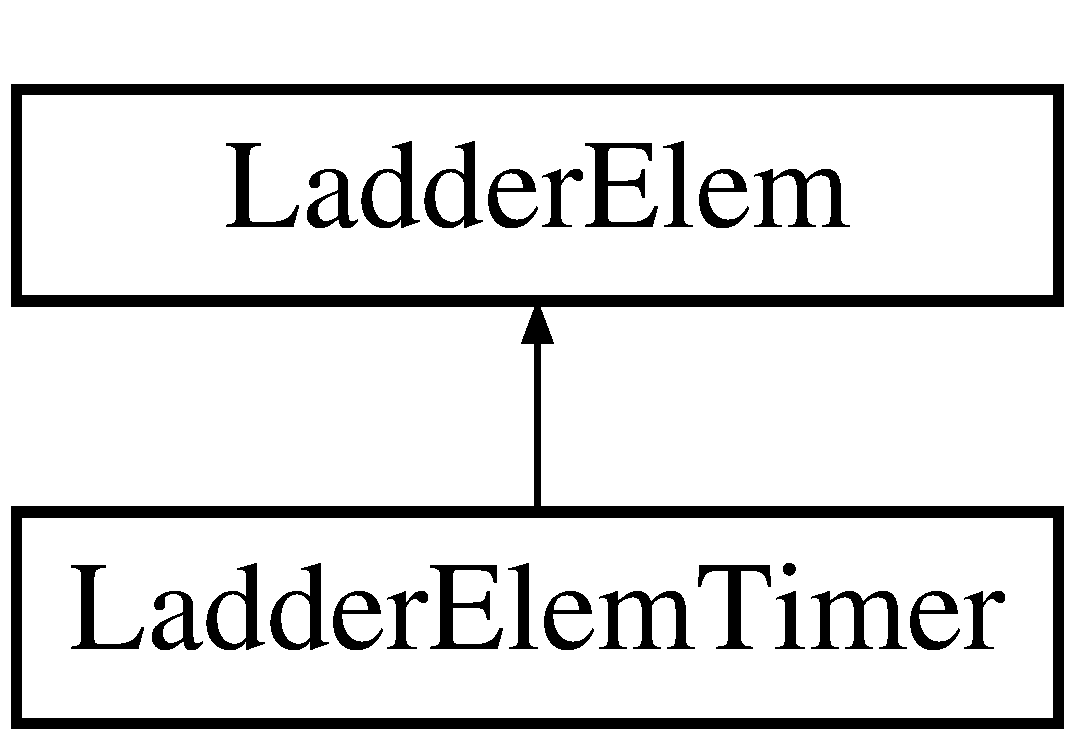
\includegraphics[height=2.000000cm]{class_ladder_elem_timer}
\end{center}
\end{figure}
\subsection*{Public Member Functions}
\begin{DoxyCompactItemize}
\item 
\hypertarget{class_ladder_elem_timer_a972ef6639f4334b17678618f4028769e}{{\bfseries Ladder\-Elem\-Timer} (\hyperlink{class_ladder_diagram}{Ladder\-Diagram} $\ast$diagram, int which)}\label{class_ladder_elem_timer_a972ef6639f4334b17678618f4028769e}

\item 
\hypertarget{class_ladder_elem_timer_aebdc4383c5a64190a8d79677d764beb4}{pair$<$ string, string $>$ {\bfseries Draw\-T\-X\-T} (void)}\label{class_ladder_elem_timer_aebdc4383c5a64190a8d79677d764beb4}

\item 
\hypertarget{class_ladder_elem_timer_ad4efb5ca163867cab8c4bf4d7110ca92}{bool {\bfseries Draw\-G\-U\-I} (bool powered\-Before, void $\ast$data)}\label{class_ladder_elem_timer_ad4efb5ca163867cab8c4bf4d7110ca92}

\item 
\hypertarget{class_ladder_elem_timer_a4bfbc6500dbe20f8d7108358e7079f48}{bool {\bfseries Show\-Dialog} (\hyperlink{struct_ladder_context}{Ladder\-Context} context)}\label{class_ladder_elem_timer_a4bfbc6500dbe20f8d7108358e7079f48}

\item 
\hypertarget{class_ladder_elem_timer_a6467b1fad85b9a327ae4e50f3940b0ba}{bool {\bfseries internal\-Generate\-Int\-Code} (\hyperlink{class_int_code}{Int\-Code} \&ic)}\label{class_ladder_elem_timer_a6467b1fad85b9a327ae4e50f3940b0ba}

\item 
\hypertarget{class_ladder_elem_timer_a2c8a9f6665c406462ae8ae39f832fe8d}{void $\ast$ {\bfseries get\-Properties} (void)}\label{class_ladder_elem_timer_a2c8a9f6665c406462ae8ae39f832fe8d}

\item 
\hypertarget{class_ladder_elem_timer_a1d7f4883d9b52788a46a4fe8e16e1d4b}{bool {\bfseries Can\-Insert} (\hyperlink{struct_ladder_context}{Ladder\-Context} context)}\label{class_ladder_elem_timer_a1d7f4883d9b52788a46a4fe8e16e1d4b}

\item 
\hypertarget{class_ladder_elem_timer_ab7e49fca6c8f3bd21b4a40a027ea28e4}{void {\bfseries do\-Post\-Insert} (void)}\label{class_ladder_elem_timer_ab7e49fca6c8f3bd21b4a40a027ea28e4}

\item 
\hypertarget{class_ladder_elem_timer_ae25150d4afc19bebc51cb8b9db6996e7}{void {\bfseries do\-Post\-Remove} (void)}\label{class_ladder_elem_timer_ae25150d4afc19bebc51cb8b9db6996e7}

\item 
\hypertarget{class_ladder_elem_timer_a947139fcd31430d17d55cdf3939cd9a5}{int {\bfseries get\-Width\-T\-X\-T} (void)}\label{class_ladder_elem_timer_a947139fcd31430d17d55cdf3939cd9a5}

\item 
\hypertarget{class_ladder_elem_timer_afddc3767d5d9c0e863fc1afe1dc529c0}{\hyperlink{class_ladder_elem}{Ladder\-Elem} $\ast$ {\bfseries Clone} (\hyperlink{class_ladder_diagram}{Ladder\-Diagram} $\ast$diagram)}\label{class_ladder_elem_timer_afddc3767d5d9c0e863fc1afe1dc529c0}

\item 
\hypertarget{class_ladder_elem_timer_a03c9b4e45920a511cd2e43f99d6b3281}{bool {\bfseries accept\-I\-O} (unsigned long id, e\-Type type)}\label{class_ladder_elem_timer_a03c9b4e45920a511cd2e43f99d6b3281}

\item 
\hypertarget{class_ladder_elem_timer_a71cb4b1ad911c2ae7fa31c72f3c5bbef}{void {\bfseries update\-I\-O} (\hyperlink{class_ladder_diagram}{Ladder\-Diagram} $\ast$owner, bool is\-Discard)}\label{class_ladder_elem_timer_a71cb4b1ad911c2ae7fa31c72f3c5bbef}

\item 
\hypertarget{class_ladder_elem_timer_a64f7131e0cb608ad6230cd13a1f15811}{e\-Type {\bfseries get\-Allowed\-Type\-I\-O} (unsigned long id)}\label{class_ladder_elem_timer_a64f7131e0cb608ad6230cd13a1f15811}

\item 
\hypertarget{class_ladder_elem_timer_ac2264b9bb9c88c2ad186a9744e7b9653}{int {\bfseries Search\-And\-Replace} (unsigned long id\-Search, string s\-New\-Text, bool is\-Replace)}\label{class_ladder_elem_timer_ac2264b9bb9c88c2ad186a9744e7b9653}

\item 
\hypertarget{class_ladder_elem_timer_a73a154763f446f468aff06e935b3275c}{bool {\bfseries internal\-Do\-Undo\-Redo} (bool Is\-Undo, bool is\-Discard, \hyperlink{struct_undo_redo_action}{Undo\-Redo\-Action} \&action)}\label{class_ladder_elem_timer_a73a154763f446f468aff06e935b3275c}

\end{DoxyCompactItemize}
\subsection*{Additional Inherited Members}


The documentation for this class was generated from the following files\-:\begin{DoxyCompactItemize}
\item 
F\-:/\-S\-V\-N/\-P\-O\-P\-Tools/Ladder\-Objects.\-h\item 
F\-:/\-S\-V\-N/\-P\-O\-P\-Tools/Ladder\-G\-U\-I.\-cpp\item 
F\-:/\-S\-V\-N/\-P\-O\-P\-Tools/Ladder\-Objects.\-cpp\end{DoxyCompactItemize}

\hypertarget{struct_ladder_elem_timer_prop}{\section{Ladder\-Elem\-Timer\-Prop Struct Reference}
\label{struct_ladder_elem_timer_prop}\index{Ladder\-Elem\-Timer\-Prop@{Ladder\-Elem\-Timer\-Prop}}
}
\subsection*{Public Attributes}
\begin{DoxyCompactItemize}
\item 
\hypertarget{struct_ladder_elem_timer_prop_abc9a55ca3001da6f68cc459cab4e416f}{pair$<$ unsigned long, int $>$ {\bfseries id\-Name}}\label{struct_ladder_elem_timer_prop_abc9a55ca3001da6f68cc459cab4e416f}

\item 
\hypertarget{struct_ladder_elem_timer_prop_a9d164e547ca02f6c011970d450b5d0a9}{int {\bfseries delay}}\label{struct_ladder_elem_timer_prop_a9d164e547ca02f6c011970d450b5d0a9}

\end{DoxyCompactItemize}


The documentation for this struct was generated from the following file\-:\begin{DoxyCompactItemize}
\item 
F\-:/\-S\-V\-N/\-P\-O\-P\-Tools/Ladder\-Objects.\-h\end{DoxyCompactItemize}

\hypertarget{class_ladder_elem_u_a_r_t}{\section{Ladder\-Elem\-U\-A\-R\-T Class Reference}
\label{class_ladder_elem_u_a_r_t}\index{Ladder\-Elem\-U\-A\-R\-T@{Ladder\-Elem\-U\-A\-R\-T}}
}
Inheritance diagram for Ladder\-Elem\-U\-A\-R\-T\-:\begin{figure}[H]
\begin{center}
\leavevmode
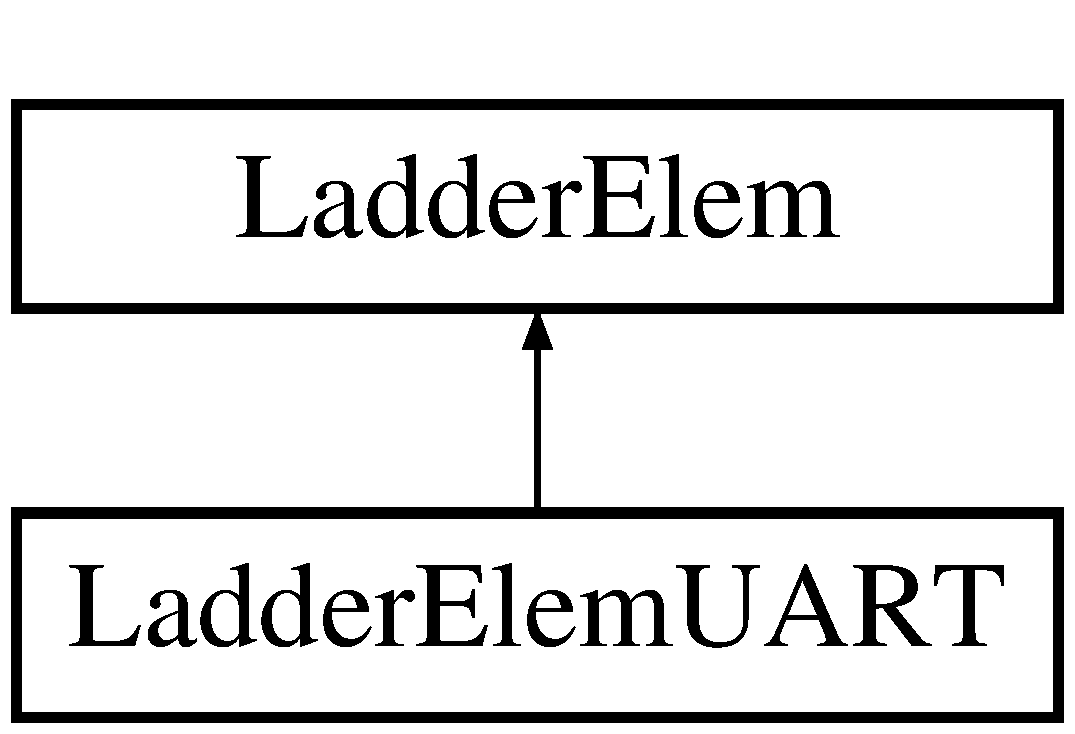
\includegraphics[height=2.000000cm]{class_ladder_elem_u_a_r_t}
\end{center}
\end{figure}
\subsection*{Public Member Functions}
\begin{DoxyCompactItemize}
\item 
\hypertarget{class_ladder_elem_u_a_r_t_aa90ba6bbbc6389d59e66f63cc44183c2}{{\bfseries Ladder\-Elem\-U\-A\-R\-T} (\hyperlink{class_ladder_diagram}{Ladder\-Diagram} $\ast$diagram, int which)}\label{class_ladder_elem_u_a_r_t_aa90ba6bbbc6389d59e66f63cc44183c2}

\item 
\hypertarget{class_ladder_elem_u_a_r_t_abcd32b88874c7c3afb50dd1acb80934c}{pair$<$ string, string $>$ {\bfseries Draw\-T\-X\-T} (void)}\label{class_ladder_elem_u_a_r_t_abcd32b88874c7c3afb50dd1acb80934c}

\item 
\hypertarget{class_ladder_elem_u_a_r_t_a5f3e5c397e1dbd324b78f7b3dc072f80}{bool {\bfseries Draw\-G\-U\-I} (bool powered\-Before, void $\ast$data)}\label{class_ladder_elem_u_a_r_t_a5f3e5c397e1dbd324b78f7b3dc072f80}

\item 
\hypertarget{class_ladder_elem_u_a_r_t_afda336a46c0c4557af403fbc1a1634cc}{bool {\bfseries Show\-Dialog} (\hyperlink{struct_ladder_context}{Ladder\-Context} context)}\label{class_ladder_elem_u_a_r_t_afda336a46c0c4557af403fbc1a1634cc}

\item 
\hypertarget{class_ladder_elem_u_a_r_t_a87872d941f862cbac3ebb9ea2b73af42}{bool {\bfseries internal\-Generate\-Int\-Code} (\hyperlink{class_int_code}{Int\-Code} \&ic)}\label{class_ladder_elem_u_a_r_t_a87872d941f862cbac3ebb9ea2b73af42}

\item 
\hypertarget{class_ladder_elem_u_a_r_t_a70124ec93c21f7e77f5dd7d1fbaeaf48}{void $\ast$ {\bfseries get\-Properties} (void)}\label{class_ladder_elem_u_a_r_t_a70124ec93c21f7e77f5dd7d1fbaeaf48}

\item 
\hypertarget{class_ladder_elem_u_a_r_t_ab7a81df9cc2177d89e6fa82910e38508}{bool {\bfseries Can\-Insert} (\hyperlink{struct_ladder_context}{Ladder\-Context} context)}\label{class_ladder_elem_u_a_r_t_ab7a81df9cc2177d89e6fa82910e38508}

\item 
\hypertarget{class_ladder_elem_u_a_r_t_a3635e56b3553f825063733705b322b89}{void {\bfseries do\-Post\-Insert} (void)}\label{class_ladder_elem_u_a_r_t_a3635e56b3553f825063733705b322b89}

\item 
\hypertarget{class_ladder_elem_u_a_r_t_a4b85ca504680171967dfb39ee80e359f}{void {\bfseries do\-Post\-Remove} (void)}\label{class_ladder_elem_u_a_r_t_a4b85ca504680171967dfb39ee80e359f}

\item 
\hypertarget{class_ladder_elem_u_a_r_t_ad71ffa48d691146d586916de0e7b02bf}{int {\bfseries get\-Width\-T\-X\-T} (void)}\label{class_ladder_elem_u_a_r_t_ad71ffa48d691146d586916de0e7b02bf}

\item 
\hypertarget{class_ladder_elem_u_a_r_t_ac2d42b30d0326d166395b94aca3e249a}{\hyperlink{class_ladder_elem}{Ladder\-Elem} $\ast$ {\bfseries Clone} (\hyperlink{class_ladder_diagram}{Ladder\-Diagram} $\ast$diagram)}\label{class_ladder_elem_u_a_r_t_ac2d42b30d0326d166395b94aca3e249a}

\item 
\hypertarget{class_ladder_elem_u_a_r_t_ad3a48046a2de0c047de4071e00be59fa}{bool {\bfseries accept\-I\-O} (unsigned long id, e\-Type type)}\label{class_ladder_elem_u_a_r_t_ad3a48046a2de0c047de4071e00be59fa}

\item 
\hypertarget{class_ladder_elem_u_a_r_t_ad2e04a485cd7f3ed365e8bd965a4799d}{void {\bfseries update\-I\-O} (\hyperlink{class_ladder_diagram}{Ladder\-Diagram} $\ast$owner, bool is\-Discard)}\label{class_ladder_elem_u_a_r_t_ad2e04a485cd7f3ed365e8bd965a4799d}

\item 
\hypertarget{class_ladder_elem_u_a_r_t_a2a0bcb8352417872a90e2a9e32bf5000}{e\-Type {\bfseries get\-Allowed\-Type\-I\-O} (unsigned long id)}\label{class_ladder_elem_u_a_r_t_a2a0bcb8352417872a90e2a9e32bf5000}

\item 
\hypertarget{class_ladder_elem_u_a_r_t_a88f9cc49d12442995b9eae37c0ac6ec3}{int {\bfseries Search\-And\-Replace} (unsigned long id\-Search, string s\-New\-Text, bool is\-Replace)}\label{class_ladder_elem_u_a_r_t_a88f9cc49d12442995b9eae37c0ac6ec3}

\item 
\hypertarget{class_ladder_elem_u_a_r_t_a28be745de6ccebf2b26848967f9eb398}{bool {\bfseries internal\-Do\-Undo\-Redo} (bool Is\-Undo, bool is\-Discard, \hyperlink{struct_undo_redo_action}{Undo\-Redo\-Action} \&action)}\label{class_ladder_elem_u_a_r_t_a28be745de6ccebf2b26848967f9eb398}

\end{DoxyCompactItemize}
\subsection*{Additional Inherited Members}


The documentation for this class was generated from the following files\-:\begin{DoxyCompactItemize}
\item 
F\-:/\-S\-V\-N/\-P\-O\-P\-Tools/Ladder\-Objects.\-h\item 
F\-:/\-S\-V\-N/\-P\-O\-P\-Tools/Ladder\-G\-U\-I.\-cpp\item 
F\-:/\-S\-V\-N/\-P\-O\-P\-Tools/Ladder\-Objects.\-cpp\end{DoxyCompactItemize}

\hypertarget{struct_ladder_elem_u_a_r_t_prop}{\section{Ladder\-Elem\-U\-A\-R\-T\-Prop Struct Reference}
\label{struct_ladder_elem_u_a_r_t_prop}\index{Ladder\-Elem\-U\-A\-R\-T\-Prop@{Ladder\-Elem\-U\-A\-R\-T\-Prop}}
}
\subsection*{Public Attributes}
\begin{DoxyCompactItemize}
\item 
\hypertarget{struct_ladder_elem_u_a_r_t_prop_aec9a340a5f28fd6ef655dfa2712d6dec}{pair$<$ unsigned long, int $>$ {\bfseries id\-Name}}\label{struct_ladder_elem_u_a_r_t_prop_aec9a340a5f28fd6ef655dfa2712d6dec}

\end{DoxyCompactItemize}


The documentation for this struct was generated from the following file\-:\begin{DoxyCompactItemize}
\item 
F\-:/\-S\-V\-N/\-P\-O\-P\-Tools/Ladder\-Objects.\-h\end{DoxyCompactItemize}

\hypertarget{class_ladder_elem_u_s_s}{\section{Ladder\-Elem\-U\-S\-S Class Reference}
\label{class_ladder_elem_u_s_s}\index{Ladder\-Elem\-U\-S\-S@{Ladder\-Elem\-U\-S\-S}}
}
Inheritance diagram for Ladder\-Elem\-U\-S\-S\-:\begin{figure}[H]
\begin{center}
\leavevmode
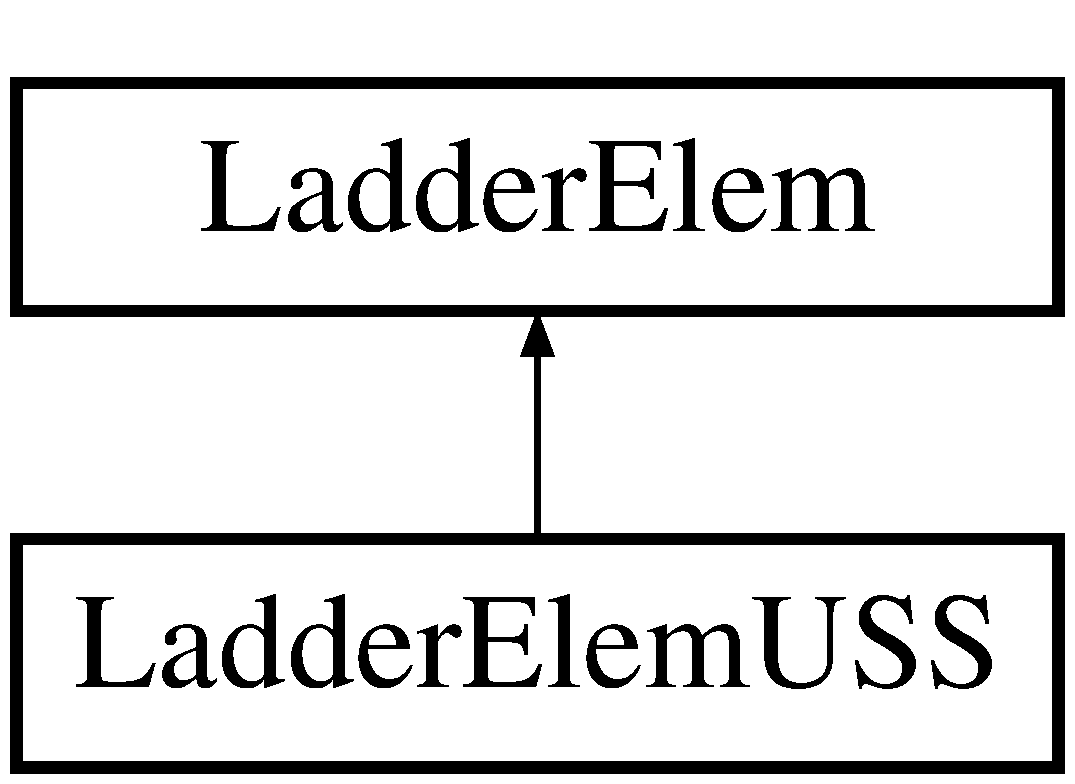
\includegraphics[height=2.000000cm]{class_ladder_elem_u_s_s}
\end{center}
\end{figure}
\subsection*{Public Member Functions}
\begin{DoxyCompactItemize}
\item 
\hypertarget{class_ladder_elem_u_s_s_a7de854ded6f0975fd04d4d06bbb45145}{{\bfseries Ladder\-Elem\-U\-S\-S} (\hyperlink{class_ladder_diagram}{Ladder\-Diagram} $\ast$diagram, int which)}\label{class_ladder_elem_u_s_s_a7de854ded6f0975fd04d4d06bbb45145}

\item 
\hypertarget{class_ladder_elem_u_s_s_a7d7177bf93f9a86c879441890413fce3}{pair$<$ string, string $>$ {\bfseries Draw\-T\-X\-T} (void)}\label{class_ladder_elem_u_s_s_a7d7177bf93f9a86c879441890413fce3}

\item 
\hypertarget{class_ladder_elem_u_s_s_a9b8b333e8e90829f7c97501aa0ac9e6f}{bool {\bfseries Draw\-G\-U\-I} (bool powered\-Before, void $\ast$data)}\label{class_ladder_elem_u_s_s_a9b8b333e8e90829f7c97501aa0ac9e6f}

\item 
\hypertarget{class_ladder_elem_u_s_s_a9a8b8cbe0f048568d595c904102d5fcc}{bool {\bfseries Show\-Dialog} (\hyperlink{struct_ladder_context}{Ladder\-Context} context)}\label{class_ladder_elem_u_s_s_a9a8b8cbe0f048568d595c904102d5fcc}

\item 
\hypertarget{class_ladder_elem_u_s_s_a5f24f96f751426a95f082509a73f38ef}{bool {\bfseries internal\-Generate\-Int\-Code} (\hyperlink{class_int_code}{Int\-Code} \&ic)}\label{class_ladder_elem_u_s_s_a5f24f96f751426a95f082509a73f38ef}

\item 
\hypertarget{class_ladder_elem_u_s_s_a85745edb24427fb54f4d5c46d5cdd2da}{void $\ast$ {\bfseries get\-Properties} (void)}\label{class_ladder_elem_u_s_s_a85745edb24427fb54f4d5c46d5cdd2da}

\item 
\hypertarget{class_ladder_elem_u_s_s_a4e830f8b6dca0c25991243e3f6b5c2a0}{bool {\bfseries Can\-Insert} (\hyperlink{struct_ladder_context}{Ladder\-Context} context)}\label{class_ladder_elem_u_s_s_a4e830f8b6dca0c25991243e3f6b5c2a0}

\item 
\hypertarget{class_ladder_elem_u_s_s_a172fc6877430b44dc87f54842509747f}{void {\bfseries do\-Post\-Insert} (void)}\label{class_ladder_elem_u_s_s_a172fc6877430b44dc87f54842509747f}

\item 
\hypertarget{class_ladder_elem_u_s_s_a573bff69cf2cb1ad09d3e2f10cd5b645}{void {\bfseries do\-Post\-Remove} (void)}\label{class_ladder_elem_u_s_s_a573bff69cf2cb1ad09d3e2f10cd5b645}

\item 
\hypertarget{class_ladder_elem_u_s_s_a642f8b5929a5053a85f4279774b861f5}{int {\bfseries get\-Width\-T\-X\-T} (void)}\label{class_ladder_elem_u_s_s_a642f8b5929a5053a85f4279774b861f5}

\item 
\hypertarget{class_ladder_elem_u_s_s_a0812bd3dd2f541e88a56002f91f4e1e4}{\hyperlink{class_ladder_elem}{Ladder\-Elem} $\ast$ {\bfseries Clone} (\hyperlink{class_ladder_diagram}{Ladder\-Diagram} $\ast$diagram)}\label{class_ladder_elem_u_s_s_a0812bd3dd2f541e88a56002f91f4e1e4}

\item 
\hypertarget{class_ladder_elem_u_s_s_a34e9eb4e183aa332679b58fe181f450a}{bool {\bfseries accept\-I\-O} (unsigned long id, e\-Type type)}\label{class_ladder_elem_u_s_s_a34e9eb4e183aa332679b58fe181f450a}

\item 
\hypertarget{class_ladder_elem_u_s_s_a33656d4784829ba0e81fbc00cef4710f}{void {\bfseries update\-I\-O} (\hyperlink{class_ladder_diagram}{Ladder\-Diagram} $\ast$owner, bool is\-Discard)}\label{class_ladder_elem_u_s_s_a33656d4784829ba0e81fbc00cef4710f}

\item 
\hypertarget{class_ladder_elem_u_s_s_a1deeaf165d62ce8effd9c461bafb67cc}{e\-Type {\bfseries get\-Allowed\-Type\-I\-O} (unsigned long id)}\label{class_ladder_elem_u_s_s_a1deeaf165d62ce8effd9c461bafb67cc}

\item 
\hypertarget{class_ladder_elem_u_s_s_a3e4810c2ae7d957d3e2a862541742b7f}{int {\bfseries Search\-And\-Replace} (unsigned long id\-Search, string s\-New\-Text, bool is\-Replace)}\label{class_ladder_elem_u_s_s_a3e4810c2ae7d957d3e2a862541742b7f}

\item 
\hypertarget{class_ladder_elem_u_s_s_aa7e10902ed859d06008ed1c3e7578816}{bool {\bfseries internal\-Do\-Undo\-Redo} (bool Is\-Undo, bool is\-Discard, \hyperlink{struct_undo_redo_action}{Undo\-Redo\-Action} \&action)}\label{class_ladder_elem_u_s_s_aa7e10902ed859d06008ed1c3e7578816}

\end{DoxyCompactItemize}
\subsection*{Additional Inherited Members}


The documentation for this class was generated from the following files\-:\begin{DoxyCompactItemize}
\item 
F\-:/\-S\-V\-N/\-P\-O\-P\-Tools/Ladder\-Objects.\-h\item 
F\-:/\-S\-V\-N/\-P\-O\-P\-Tools/Ladder\-G\-U\-I.\-cpp\item 
F\-:/\-S\-V\-N/\-P\-O\-P\-Tools/Ladder\-Objects.\-cpp\end{DoxyCompactItemize}

\hypertarget{struct_ladder_elem_u_s_s_prop}{\section{Ladder\-Elem\-U\-S\-S\-Prop Struct Reference}
\label{struct_ladder_elem_u_s_s_prop}\index{Ladder\-Elem\-U\-S\-S\-Prop@{Ladder\-Elem\-U\-S\-S\-Prop}}
}
\subsection*{Public Attributes}
\begin{DoxyCompactItemize}
\item 
\hypertarget{struct_ladder_elem_u_s_s_prop_a2df334662adb55e84df2abc9cd6c057b}{pair$<$ unsigned long, int $>$ {\bfseries id\-Name}}\label{struct_ladder_elem_u_s_s_prop_a2df334662adb55e84df2abc9cd6c057b}

\item 
\hypertarget{struct_ladder_elem_u_s_s_prop_a0ebf189f7d975487a732f42fcf2c7a2c}{int {\bfseries id}}\label{struct_ladder_elem_u_s_s_prop_a0ebf189f7d975487a732f42fcf2c7a2c}

\item 
\hypertarget{struct_ladder_elem_u_s_s_prop_a5ea1622232b1fff71fa9aaf986abb2b0}{int {\bfseries parameter}}\label{struct_ladder_elem_u_s_s_prop_a5ea1622232b1fff71fa9aaf986abb2b0}

\item 
\hypertarget{struct_ladder_elem_u_s_s_prop_a626a4bff485f1957006f9e0e13bee190}{int {\bfseries parameter\-\_\-set}}\label{struct_ladder_elem_u_s_s_prop_a626a4bff485f1957006f9e0e13bee190}

\item 
\hypertarget{struct_ladder_elem_u_s_s_prop_aceb20ca23763517667174908954adf35}{int {\bfseries index}}\label{struct_ladder_elem_u_s_s_prop_aceb20ca23763517667174908954adf35}

\end{DoxyCompactItemize}


The documentation for this struct was generated from the following file\-:\begin{DoxyCompactItemize}
\item 
F\-:/\-S\-V\-N/\-P\-O\-P\-Tools/Ladder\-Objects.\-h\end{DoxyCompactItemize}

\hypertarget{class_ladder_elem_x}{\section{Ladder\-Elem\-X Class Reference}
\label{class_ladder_elem_x}\index{Ladder\-Elem\-X@{Ladder\-Elem\-X}}
}
Inheritance diagram for Ladder\-Elem\-X\-:\begin{figure}[H]
\begin{center}
\leavevmode
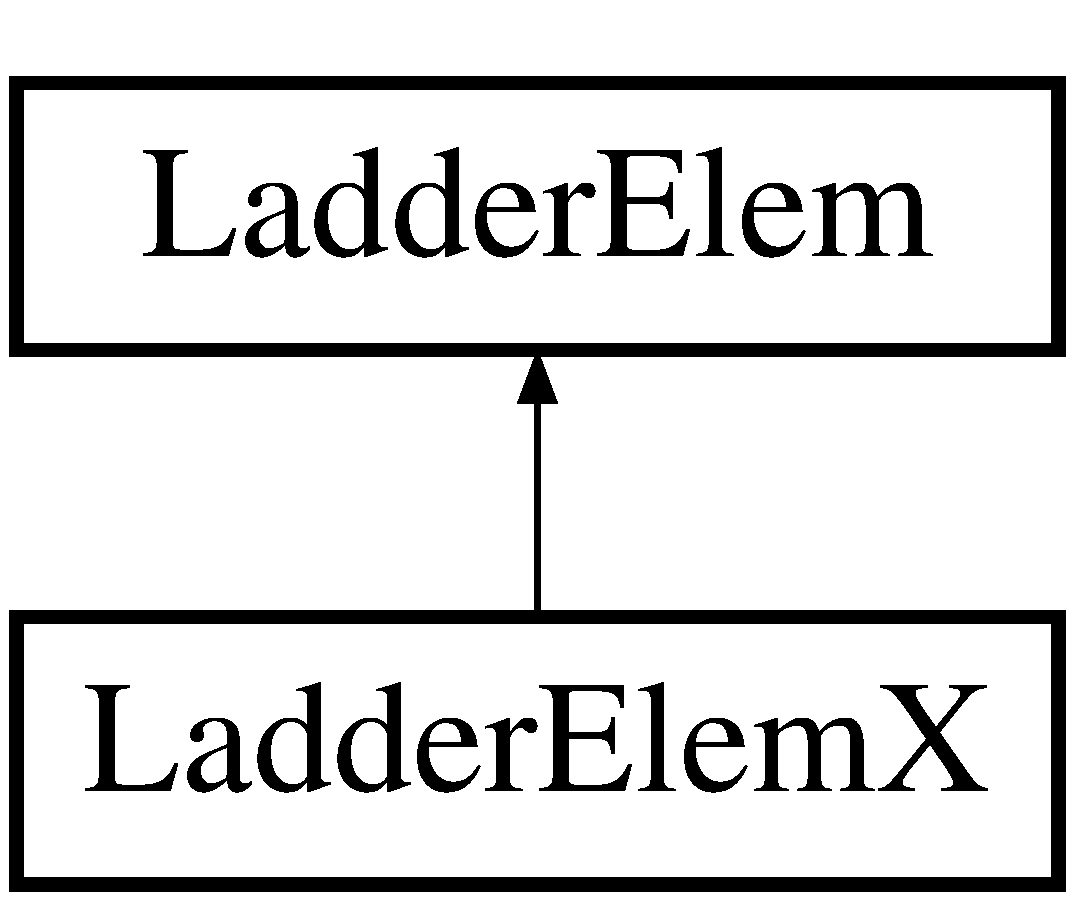
\includegraphics[height=2.000000cm]{class_ladder_elem_x}
\end{center}
\end{figure}
\subsection*{Public Member Functions}
\begin{DoxyCompactItemize}
\item 
\hypertarget{class_ladder_elem_x_a726b3527dd25b62998689a5bca6c6ffa}{{\bfseries Ladder\-Elem\-X} (\hyperlink{class_ladder_diagram}{Ladder\-Diagram} $\ast$diagram)}\label{class_ladder_elem_x_a726b3527dd25b62998689a5bca6c6ffa}

\item 
\hypertarget{class_ladder_elem_x_a3997e9e51ad4ece4ae549d91734b3ce0}{pair$<$ string, string $>$ {\bfseries Draw\-T\-X\-T} (void)}\label{class_ladder_elem_x_a3997e9e51ad4ece4ae549d91734b3ce0}

\item 
\hypertarget{class_ladder_elem_x_a0d5dc08c9419d9b497aa811d3671e657}{bool {\bfseries Draw\-G\-U\-I} (bool powered\-Before, void $\ast$data)}\label{class_ladder_elem_x_a0d5dc08c9419d9b497aa811d3671e657}

\item 
\hypertarget{class_ladder_elem_x_a074421a0c2ef0d04439df37d1bc0f855}{bool {\bfseries Show\-Dialog} (\hyperlink{struct_ladder_context}{Ladder\-Context} context)}\label{class_ladder_elem_x_a074421a0c2ef0d04439df37d1bc0f855}

\item 
\hypertarget{class_ladder_elem_x_a4ec8e07456fbd7bb196a34d490521aff}{bool {\bfseries internal\-Generate\-Int\-Code} (\hyperlink{class_int_code}{Int\-Code} \&ic)}\label{class_ladder_elem_x_a4ec8e07456fbd7bb196a34d490521aff}

\item 
\hypertarget{class_ladder_elem_x_a87a0c35b8b51796e0382623369dc44ef}{void $\ast$ {\bfseries get\-Properties} (void)}\label{class_ladder_elem_x_a87a0c35b8b51796e0382623369dc44ef}

\item 
\hypertarget{class_ladder_elem_x_aa7745dceaf8a0300e109882253ba9664}{bool {\bfseries Can\-Insert} (\hyperlink{struct_ladder_context}{Ladder\-Context} context)}\label{class_ladder_elem_x_aa7745dceaf8a0300e109882253ba9664}

\item 
\hypertarget{class_ladder_elem_x_a311151da1e6e01dfbb9a66aaa7f5264c}{void {\bfseries do\-Post\-Insert} (void)}\label{class_ladder_elem_x_a311151da1e6e01dfbb9a66aaa7f5264c}

\item 
\hypertarget{class_ladder_elem_x_a9ab46f8d90c4521361c183ade89f8e99}{void {\bfseries do\-Post\-Remove} (void)}\label{class_ladder_elem_x_a9ab46f8d90c4521361c183ade89f8e99}

\item 
\hypertarget{class_ladder_elem_x_a545b95621f51fd75c2df5f8d7d0293a3}{int {\bfseries get\-Width\-T\-X\-T} (void)}\label{class_ladder_elem_x_a545b95621f51fd75c2df5f8d7d0293a3}

\item 
\hypertarget{class_ladder_elem_x_a543923c0ff29f8ccb1dde76e8665cb1c}{\hyperlink{class_ladder_elem}{Ladder\-Elem} $\ast$ {\bfseries Clone} (\hyperlink{class_ladder_diagram}{Ladder\-Diagram} $\ast$diagram)}\label{class_ladder_elem_x_a543923c0ff29f8ccb1dde76e8665cb1c}

\item 
\hypertarget{class_ladder_elem_x_a7f2294914e3348c6615dea8f23a10c7d}{bool {\bfseries accept\-I\-O} (unsigned long id, e\-Type type)}\label{class_ladder_elem_x_a7f2294914e3348c6615dea8f23a10c7d}

\item 
\hypertarget{class_ladder_elem_x_a40965643c88b60082ec5ad9f890a3b20}{void {\bfseries update\-I\-O} (\hyperlink{class_ladder_diagram}{Ladder\-Diagram} $\ast$owner, bool is\-Discard)}\label{class_ladder_elem_x_a40965643c88b60082ec5ad9f890a3b20}

\item 
\hypertarget{class_ladder_elem_x_a57a585b65c60d6ad25e42d71f2b188d8}{e\-Type {\bfseries get\-Allowed\-Type\-I\-O} (unsigned long id)}\label{class_ladder_elem_x_a57a585b65c60d6ad25e42d71f2b188d8}

\item 
\hypertarget{class_ladder_elem_x_a0d68df2f5a0ed16f12b658f97c815b8f}{int {\bfseries Search\-And\-Replace} (unsigned long id\-Search, string s\-New\-Text, bool is\-Replace)}\label{class_ladder_elem_x_a0d68df2f5a0ed16f12b658f97c815b8f}

\item 
\hypertarget{class_ladder_elem_x_a288f2dd6f82e09798266d851fee3a446}{bool {\bfseries internal\-Do\-Undo\-Redo} (bool Is\-Undo, bool is\-Discard, \hyperlink{struct_undo_redo_action}{Undo\-Redo\-Action} \&action)}\label{class_ladder_elem_x_a288f2dd6f82e09798266d851fee3a446}

\end{DoxyCompactItemize}
\subsection*{Additional Inherited Members}


The documentation for this class was generated from the following files\-:\begin{DoxyCompactItemize}
\item 
F\-:/\-S\-V\-N/\-P\-O\-P\-Tools/Ladder\-Objects.\-h\item 
F\-:/\-S\-V\-N/\-P\-O\-P\-Tools/Ladder\-G\-U\-I.\-cpp\item 
F\-:/\-S\-V\-N/\-P\-O\-P\-Tools/Ladder\-Objects.\-cpp\end{DoxyCompactItemize}

\hypertarget{struct_ladder_elem_x_prop}{\section{Ladder\-Elem\-X\-Prop Struct Reference}
\label{struct_ladder_elem_x_prop}\index{Ladder\-Elem\-X\-Prop@{Ladder\-Elem\-X\-Prop}}
}


The documentation for this struct was generated from the following file\-:\begin{DoxyCompactItemize}
\item 
F\-:/\-S\-V\-N/\-P\-O\-P\-Tools/Ladder\-Objects.\-h\end{DoxyCompactItemize}

\hypertarget{class_ladder_elem_yaskawa}{\section{Ladder\-Elem\-Yaskawa Class Reference}
\label{class_ladder_elem_yaskawa}\index{Ladder\-Elem\-Yaskawa@{Ladder\-Elem\-Yaskawa}}
}
Inheritance diagram for Ladder\-Elem\-Yaskawa\-:\begin{figure}[H]
\begin{center}
\leavevmode
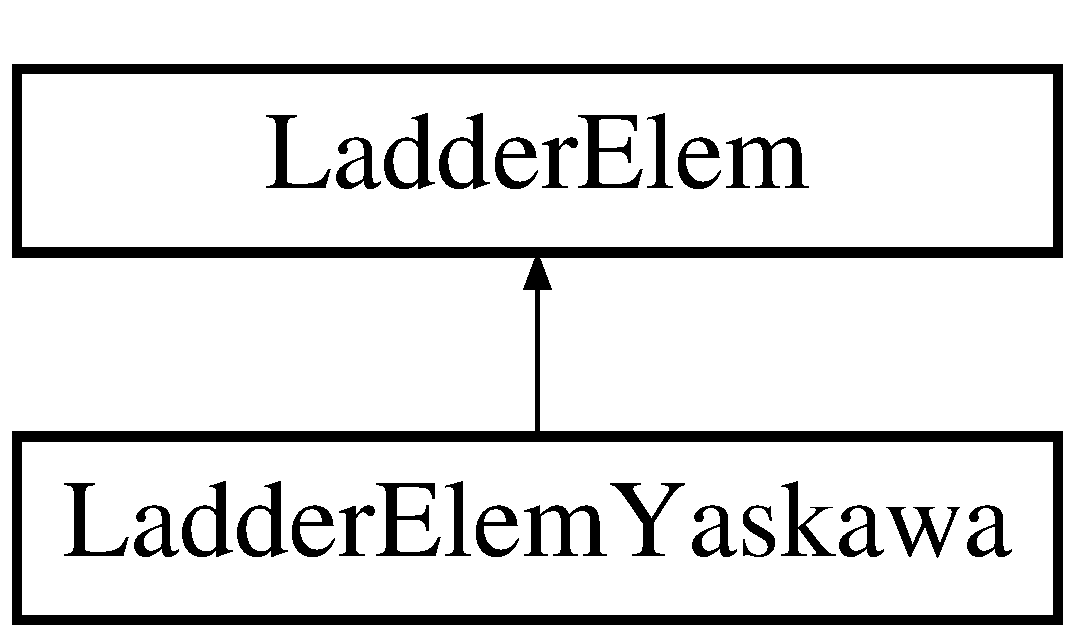
\includegraphics[height=2.000000cm]{class_ladder_elem_yaskawa}
\end{center}
\end{figure}
\subsection*{Public Member Functions}
\begin{DoxyCompactItemize}
\item 
\hypertarget{class_ladder_elem_yaskawa_ad67d0055087d4bd8088acb214760fa6f}{{\bfseries Ladder\-Elem\-Yaskawa} (\hyperlink{class_ladder_diagram}{Ladder\-Diagram} $\ast$diagram, int which)}\label{class_ladder_elem_yaskawa_ad67d0055087d4bd8088acb214760fa6f}

\item 
\hypertarget{class_ladder_elem_yaskawa_a23677d298d3ff7392165596adff0ff02}{pair$<$ string, string $>$ {\bfseries Draw\-T\-X\-T} (void)}\label{class_ladder_elem_yaskawa_a23677d298d3ff7392165596adff0ff02}

\item 
\hypertarget{class_ladder_elem_yaskawa_aa66fa585297f2673627caa0aea9c5b5d}{bool {\bfseries Draw\-G\-U\-I} (bool powered\-Before, void $\ast$data)}\label{class_ladder_elem_yaskawa_aa66fa585297f2673627caa0aea9c5b5d}

\item 
\hypertarget{class_ladder_elem_yaskawa_ac7cffe3d069c324c4f0de871876394a8}{bool {\bfseries Show\-Dialog} (\hyperlink{struct_ladder_context}{Ladder\-Context} context)}\label{class_ladder_elem_yaskawa_ac7cffe3d069c324c4f0de871876394a8}

\item 
\hypertarget{class_ladder_elem_yaskawa_affebaaf8a63e2eee0cf5afb962242ead}{bool {\bfseries internal\-Generate\-Int\-Code} (\hyperlink{class_int_code}{Int\-Code} \&ic)}\label{class_ladder_elem_yaskawa_affebaaf8a63e2eee0cf5afb962242ead}

\item 
\hypertarget{class_ladder_elem_yaskawa_aea09458057dd6f47b051df180e34043a}{void $\ast$ {\bfseries get\-Properties} (void)}\label{class_ladder_elem_yaskawa_aea09458057dd6f47b051df180e34043a}

\item 
\hypertarget{class_ladder_elem_yaskawa_a94995c0dc03048e8cb8cfc78f2bf40fe}{bool {\bfseries Can\-Insert} (\hyperlink{struct_ladder_context}{Ladder\-Context} context)}\label{class_ladder_elem_yaskawa_a94995c0dc03048e8cb8cfc78f2bf40fe}

\item 
\hypertarget{class_ladder_elem_yaskawa_af3814181d768377f9ee1f2396cf10b6b}{void {\bfseries do\-Post\-Insert} (void)}\label{class_ladder_elem_yaskawa_af3814181d768377f9ee1f2396cf10b6b}

\item 
\hypertarget{class_ladder_elem_yaskawa_a3867950337ad3c36ca7e8ecc82777d4c}{void {\bfseries do\-Post\-Remove} (void)}\label{class_ladder_elem_yaskawa_a3867950337ad3c36ca7e8ecc82777d4c}

\item 
\hypertarget{class_ladder_elem_yaskawa_adad4cc71e931510401fd7cb68486e87c}{int {\bfseries get\-Width\-T\-X\-T} (void)}\label{class_ladder_elem_yaskawa_adad4cc71e931510401fd7cb68486e87c}

\item 
\hypertarget{class_ladder_elem_yaskawa_a9add9edaf2bf9270a8e306cc57320fe4}{\hyperlink{class_ladder_elem}{Ladder\-Elem} $\ast$ {\bfseries Clone} (\hyperlink{class_ladder_diagram}{Ladder\-Diagram} $\ast$diagram)}\label{class_ladder_elem_yaskawa_a9add9edaf2bf9270a8e306cc57320fe4}

\item 
\hypertarget{class_ladder_elem_yaskawa_a73b9a3b5f79b4f1c42670ebf7f9687bf}{bool {\bfseries accept\-I\-O} (unsigned long id, e\-Type type)}\label{class_ladder_elem_yaskawa_a73b9a3b5f79b4f1c42670ebf7f9687bf}

\item 
\hypertarget{class_ladder_elem_yaskawa_ae748ef31bc220d83c2a8b1efabdb24b5}{void {\bfseries update\-I\-O} (\hyperlink{class_ladder_diagram}{Ladder\-Diagram} $\ast$owner, bool is\-Discard)}\label{class_ladder_elem_yaskawa_ae748ef31bc220d83c2a8b1efabdb24b5}

\item 
\hypertarget{class_ladder_elem_yaskawa_a475753722515e3735ba90a0142412064}{e\-Type {\bfseries get\-Allowed\-Type\-I\-O} (unsigned long id)}\label{class_ladder_elem_yaskawa_a475753722515e3735ba90a0142412064}

\item 
\hypertarget{class_ladder_elem_yaskawa_a6965bb96294a1dde4e3b622160340c2f}{int {\bfseries Search\-And\-Replace} (unsigned long id\-Search, string s\-New\-Text, bool is\-Replace)}\label{class_ladder_elem_yaskawa_a6965bb96294a1dde4e3b622160340c2f}

\item 
\hypertarget{class_ladder_elem_yaskawa_ad559b6dc3bad47afed4a611e0344f636}{bool {\bfseries internal\-Do\-Undo\-Redo} (bool Is\-Undo, bool is\-Discard, \hyperlink{struct_undo_redo_action}{Undo\-Redo\-Action} \&action)}\label{class_ladder_elem_yaskawa_ad559b6dc3bad47afed4a611e0344f636}

\end{DoxyCompactItemize}
\subsection*{Additional Inherited Members}


The documentation for this class was generated from the following files\-:\begin{DoxyCompactItemize}
\item 
F\-:/\-S\-V\-N/\-P\-O\-P\-Tools/Ladder\-Objects.\-h\item 
F\-:/\-S\-V\-N/\-P\-O\-P\-Tools/Ladder\-G\-U\-I.\-cpp\item 
F\-:/\-S\-V\-N/\-P\-O\-P\-Tools/Ladder\-Objects.\-cpp\end{DoxyCompactItemize}

\hypertarget{struct_ladder_elem_yaskawa_prop}{\section{Ladder\-Elem\-Yaskawa\-Prop Struct Reference}
\label{struct_ladder_elem_yaskawa_prop}\index{Ladder\-Elem\-Yaskawa\-Prop@{Ladder\-Elem\-Yaskawa\-Prop}}
}
\subsection*{Public Attributes}
\begin{DoxyCompactItemize}
\item 
\hypertarget{struct_ladder_elem_yaskawa_prop_a4f62c33ac2edc24466ca431a636e3704}{pair$<$ unsigned long, int $>$ {\bfseries id\-Var}}\label{struct_ladder_elem_yaskawa_prop_a4f62c33ac2edc24466ca431a636e3704}

\item 
\hypertarget{struct_ladder_elem_yaskawa_prop_ab36d0e6e81bf6ddf47b0d410de4fc7c5}{int {\bfseries id}}\label{struct_ladder_elem_yaskawa_prop_ab36d0e6e81bf6ddf47b0d410de4fc7c5}

\item 
\hypertarget{struct_ladder_elem_yaskawa_prop_acbe03ef17b6b1e664e63de2665bb2175}{string {\bfseries txt}}\label{struct_ladder_elem_yaskawa_prop_acbe03ef17b6b1e664e63de2665bb2175}

\end{DoxyCompactItemize}


The documentation for this struct was generated from the following file\-:\begin{DoxyCompactItemize}
\item 
F\-:/\-S\-V\-N/\-P\-O\-P\-Tools/Ladder\-Objects.\-h\end{DoxyCompactItemize}

\hypertarget{class_ladder_g_u_i}{\section{Ladder\-G\-U\-I Class Reference}
\label{class_ladder_g_u_i}\index{Ladder\-G\-U\-I@{Ladder\-G\-U\-I}}
}
Inheritance diagram for Ladder\-G\-U\-I\-:\begin{figure}[H]
\begin{center}
\leavevmode
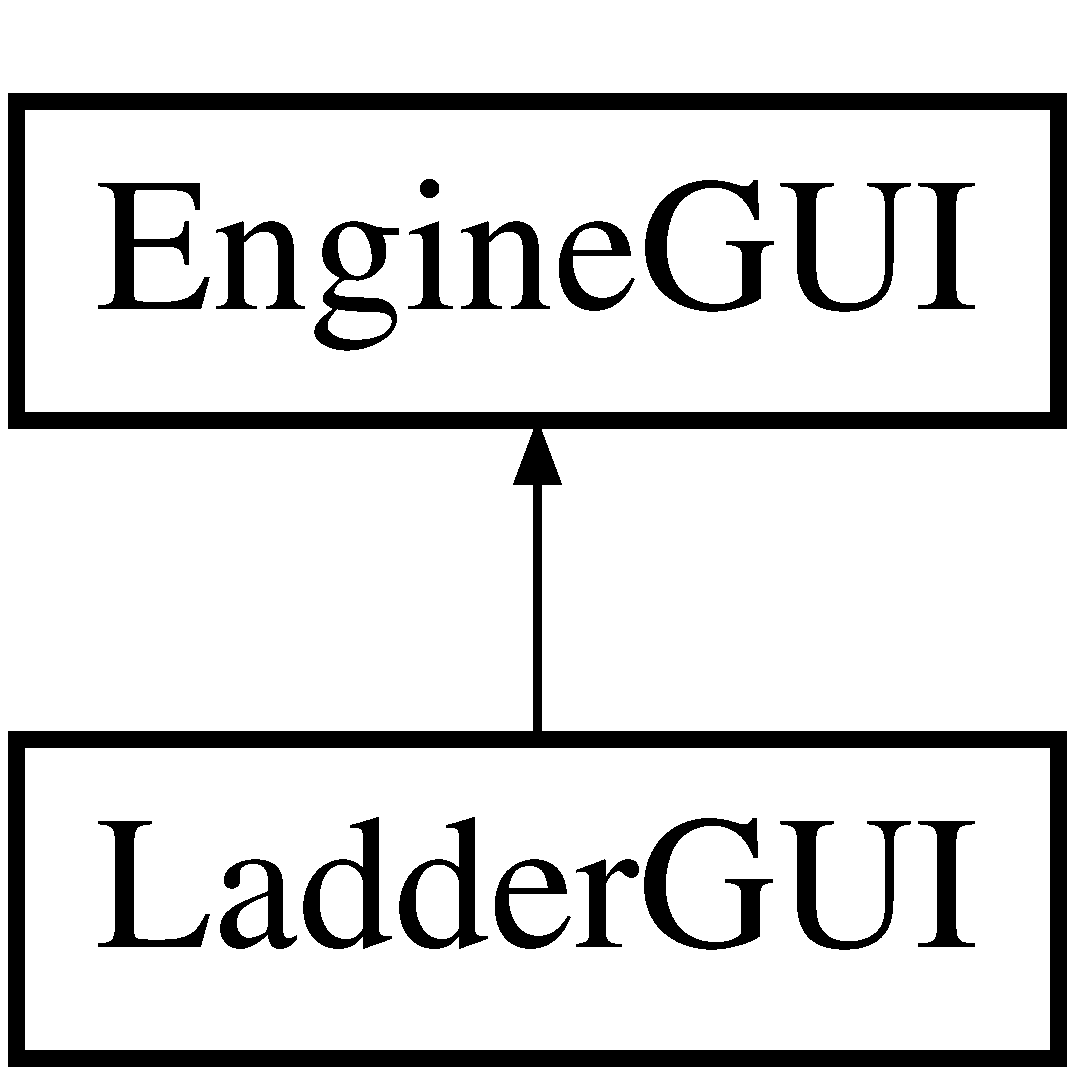
\includegraphics[height=2.000000cm]{class_ladder_g_u_i}
\end{center}
\end{figure}
\subsection*{Public Member Functions}
\begin{DoxyCompactItemize}
\item 
\hypertarget{class_ladder_g_u_i_a0b0c55332cf4f1ebfbe5b87fda50a3bc}{R\-E\-C\-T {\bfseries get\-R\-E\-C\-T} (P\-O\-I\-N\-T Start, P\-O\-I\-N\-T Size)}\label{class_ladder_g_u_i_a0b0c55332cf4f1ebfbe5b87fda50a3bc}

\item 
\hypertarget{class_ladder_g_u_i_a8426c5bd79550bcf490a0ce29a66fd4d}{P\-O\-I\-N\-T {\bfseries get\-Grid\-Size} (void)}\label{class_ladder_g_u_i_a8426c5bd79550bcf490a0ce29a66fd4d}

\item 
\hypertarget{class_ladder_g_u_i_a2e604e47d26e0897791c3b9c682f51e5}{P\-O\-I\-N\-T {\bfseries get\-Center} (R\-E\-C\-T r)}\label{class_ladder_g_u_i_a2e604e47d26e0897791c3b9c682f51e5}

\item 
\hypertarget{class_ladder_g_u_i_ae1b37dcde73b507f8536fecd271557ba}{bool {\bfseries Is\-Expanded} (\hyperlink{class_ladder_elem}{Ladder\-Elem} $\ast$elem)}\label{class_ladder_g_u_i_ae1b37dcde73b507f8536fecd271557ba}

\item 
\hypertarget{class_ladder_g_u_i_a4510c9be8e36838cc79460a37c35f5bf}{void {\bfseries set\-Mouse\-Position} (P\-O\-I\-N\-T xy)}\label{class_ladder_g_u_i_a4510c9be8e36838cc79460a37c35f5bf}

\item 
\hypertarget{class_ladder_g_u_i_a41d24a0adc071b4bd2b020f53f6452f3}{void {\bfseries set\-Diagram\-Size} (P\-O\-I\-N\-T size)}\label{class_ladder_g_u_i_a41d24a0adc071b4bd2b020f53f6452f3}

\item 
\hypertarget{class_ladder_g_u_i_ae44faaf1fc7153aa0859c001d1293c60}{P\-O\-I\-N\-T {\bfseries get\-Diagram\-Size} (void)}\label{class_ladder_g_u_i_ae44faaf1fc7153aa0859c001d1293c60}

\item 
\hypertarget{class_ladder_g_u_i_adaddaa4612d67211fc6c8ba7f76c2ae4}{void {\bfseries Draw\-Init} (void)}\label{class_ladder_g_u_i_adaddaa4612d67211fc6c8ba7f76c2ae4}

\item 
\hypertarget{class_ladder_g_u_i_aac5fdbae15dc7d7fa4f222470e9146f2}{void {\bfseries Draw\-Start} (int Offset\-X, int Offset\-Y)}\label{class_ladder_g_u_i_aac5fdbae15dc7d7fa4f222470e9146f2}

\item 
\hypertarget{class_ladder_g_u_i_a8d54533c231efe46da6f72cbba19993e}{void {\bfseries Draw\-End} (void)}\label{class_ladder_g_u_i_a8d54533c231efe46da6f72cbba19993e}

\item 
\hypertarget{class_ladder_g_u_i_a9f8ff54b68a9fcd5387d4fa144e0be01}{void {\bfseries Need\-Redraw} (bool is\-Redraw\-Needed)}\label{class_ladder_g_u_i_a9f8ff54b68a9fcd5387d4fa144e0be01}

\item 
\hypertarget{class_ladder_g_u_i_a0733995d83f98f39dc9a1ea02f14b6a3}{bool {\bfseries get\-Need\-Full\-Redraw} (void)}\label{class_ladder_g_u_i_a0733995d83f98f39dc9a1ea02f14b6a3}

\item 
\hypertarget{class_ladder_g_u_i_a7791bdc080c9f75639d81ea40930bfd9}{void {\bfseries register\-Element\-Area} (\hyperlink{class_ladder_elem}{Ladder\-Elem} $\ast$elem, P\-O\-I\-N\-T start, P\-O\-I\-N\-T size)}\label{class_ladder_g_u_i_a7791bdc080c9f75639d81ea40930bfd9}

\item 
\hypertarget{class_ladder_g_u_i_a5660af98b03574a4e5f81631d5fa9a28}{void {\bfseries Draw\-Element\-Box} (\hyperlink{class_ladder_elem}{Ladder\-Elem} $\ast$elem, int Selected\-State, P\-O\-I\-N\-T Start\-Top\-Left, bool powered\-Before)}\label{class_ladder_g_u_i_a5660af98b03574a4e5f81631d5fa9a28}

\item 
\hypertarget{class_ladder_g_u_i_a581ce8afeebc92fd1d8f3e26b8acf7f5}{R\-E\-C\-T {\bfseries Draw\-Element\-Box} (\hyperlink{class_ladder_elem}{Ladder\-Elem} $\ast$elem, int Selected\-State, P\-O\-I\-N\-T Start\-Top\-Left, P\-O\-I\-N\-T Grid\-Size, string Elem\-Name, bool Show\-Expand, bool powered\-Before)}\label{class_ladder_g_u_i_a581ce8afeebc92fd1d8f3e26b8acf7f5}

\item 
\hypertarget{class_ladder_g_u_i_ac700f6ed3bcaaed07796b5be82c4a1ae}{void {\bfseries Draw\-Element\-Box} (\hyperlink{class_ladder_elem}{Ladder\-Elem} $\ast$elem, int Selected\-State, P\-O\-I\-N\-T Start\-Top\-Left, pair$<$ string, string $>$ txt, bool powered\-Before)}\label{class_ladder_g_u_i_ac700f6ed3bcaaed07796b5be82c4a1ae}

\item 
\hypertarget{class_ladder_g_u_i_a10e3a143a7a9fff23031f0ff65168f15}{R\-E\-C\-T {\bfseries Draw\-Element\-Bar} (\hyperlink{class_ladder_elem}{Ladder\-Elem} $\ast$elem, int Selected\-State, int Start\-Grid\-Y, int Grid\-Height)}\label{class_ladder_g_u_i_a10e3a143a7a9fff23031f0ff65168f15}

\item 
\hypertarget{class_ladder_g_u_i_a6a50a402954c5a206744291b53b48cd5}{void {\bfseries Draw\-Dialog\-Box} (void)}\label{class_ladder_g_u_i_a6a50a402954c5a206744291b53b48cd5}

\item 
\hypertarget{class_ladder_g_u_i_a067c37178b174a5923371e9ac7758756}{vector$<$ R\-E\-C\-T $>$ {\bfseries Draw\-Expanded\-Items} (\hyperlink{structt_ladder_color_group}{t\-Ladder\-Color\-Group} cg, R\-E\-C\-T r, P\-O\-I\-N\-T Grid\-Size, unsigned int Grid\-Offset, vector$<$ t\-Expanded\-Item $>$ items)}\label{class_ladder_g_u_i_a067c37178b174a5923371e9ac7758756}

\item 
\hypertarget{class_ladder_g_u_i_a6b74a8479f0f38925f1185f05d34e78a}{void {\bfseries add\-Control\-List} (\hyperlink{class_ladder_elem}{Ladder\-Elem} $\ast$elem, R\-E\-C\-T r, \hyperlink{structt_control_list}{t\-Control\-List} list)}\label{class_ladder_g_u_i_a6b74a8479f0f38925f1185f05d34e78a}

\item 
\hypertarget{class_ladder_g_u_i_ae2b0716310eadc106c8730d7706b287c}{e\-Reply {\bfseries Show\-Dialog} (e\-Dialog\-Type type, bool has\-Cancel, char $\ast$title, char $\ast$message)}\label{class_ladder_g_u_i_ae2b0716310eadc106c8730d7706b287c}

\item 
\hypertarget{class_ladder_g_u_i_a762cb36ef9f9102f89d3e0b173bddb75}{\hyperlink{structt_dialog_data}{t\-Dialog\-Data} {\bfseries get\-Dialog\-Data} (void)}\label{class_ladder_g_u_i_a762cb36ef9f9102f89d3e0b173bddb75}

\item 
\hypertarget{class_ladder_g_u_i_a4e369f5fcdcee6201cb3dfc3f698baad}{bool {\bfseries Is\-Dialog\-Active} (void)}\label{class_ladder_g_u_i_a4e369f5fcdcee6201cb3dfc3f698baad}

\item 
\hypertarget{class_ladder_g_u_i_a0a96784ef888dada1ab256521b2b7cee}{void {\bfseries set\-Dialog\-Active\-Button} (bool is\-Next)}\label{class_ladder_g_u_i_a0a96784ef888dada1ab256521b2b7cee}

\item 
\hypertarget{class_ladder_g_u_i_a34f680c13d12768f5a0a2865d546876f}{void {\bfseries Dialog\-Confirm} (void)}\label{class_ladder_g_u_i_a34f680c13d12768f5a0a2865d546876f}

\item 
\hypertarget{class_ladder_g_u_i_a3257f215cfbd8e01c2807a722d480ff3}{void {\bfseries Dialog\-Cancel} (void)}\label{class_ladder_g_u_i_a3257f215cfbd8e01c2807a722d480ff3}

\item 
\hypertarget{class_ladder_g_u_i_a9a64f28b43d31216367327f298aa4b34}{\hyperlink{structt_wire}{t\-Wire} {\bfseries Draw\-Wire} (P\-O\-I\-N\-T Start\-Point, P\-O\-I\-N\-T End\-Point, bool powered\-Before)}\label{class_ladder_g_u_i_a9a64f28b43d31216367327f298aa4b34}

\item 
\hypertarget{class_ladder_g_u_i_af4fa1d4b562913cc18ae0616bdb7a6c7}{void {\bfseries add\-Connection\-Dot} (P\-O\-I\-N\-T p, bool is\-Powered, bool is\-Forced)}\label{class_ladder_g_u_i_af4fa1d4b562913cc18ae0616bdb7a6c7}

\item 
\hypertarget{class_ladder_g_u_i_a052750a31040fb8b7f82abf346e9ce74}{void {\bfseries Mouse\-Click} (int x, int y, bool is\-Down, bool is\-Double)}\label{class_ladder_g_u_i_a052750a31040fb8b7f82abf346e9ce74}

\item 
\hypertarget{class_ladder_g_u_i_a4e3d8b08d392f59bfc1f82f8bd55b95e}{\hyperlink{class_ladder_elem}{Ladder\-Elem} $\ast$ {\bfseries Search\-Element} (\hyperlink{class_ladder_elem}{Ladder\-Elem} $\ast$ref, e\-Move\-Cursor move\-To)}\label{class_ladder_g_u_i_a4e3d8b08d392f59bfc1f82f8bd55b95e}

\item 
\hypertarget{class_ladder_g_u_i_a1874723313539566c551d3d30fcecf67}{R\-E\-C\-T {\bfseries get\-Elem\-Area} (\hyperlink{class_ladder_elem}{Ladder\-Elem} $\ast$elem)}\label{class_ladder_g_u_i_a1874723313539566c551d3d30fcecf67}

\item 
\hypertarget{class_ladder_g_u_i_a4d839417f15ecd7348ff857a8c95da2f}{void {\bfseries Add\-Command} (\hyperlink{structt_command_source}{t\-Command\-Source} source, R\-E\-C\-T region, bool($\ast$fnc)(\hyperlink{structt_command_source}{t\-Command\-Source}, void $\ast$), void $\ast$data, bool is\-Double\-Click, bool is\-Simulation\-Mode, bool is\-Dialog\-Command=false)}\label{class_ladder_g_u_i_a4d839417f15ecd7348ff857a8c95da2f}

\item 
\hypertarget{class_ladder_g_u_i_ad38f2b4e99a87eb6f8c36bb417fba746}{void {\bfseries Cmd\-Expand} (\hyperlink{class_ladder_elem}{Ladder\-Elem} $\ast$elem)}\label{class_ladder_g_u_i_ad38f2b4e99a87eb6f8c36bb417fba746}

\item 
\hypertarget{class_ladder_g_u_i_a90c2a03c8c81b76b4ae620decc996ead}{void {\bfseries set\-Ladder\-Colors} (\hyperlink{structt_ladder_colors}{t\-Ladder\-Colors} colors, bool is\-Mode\-Simulation)}\label{class_ladder_g_u_i_a90c2a03c8c81b76b4ae620decc996ead}

\item 
\hypertarget{class_ladder_g_u_i_afb9e72e9c42c974660b7548258e8bc75}{\hyperlink{structt_ladder_colors}{t\-Ladder\-Colors} {\bfseries get\-Ladder\-Colors} (void)}\label{class_ladder_g_u_i_afb9e72e9c42c974660b7548258e8bc75}

\item 
\hypertarget{class_ladder_g_u_i_a8ae195d8e744527a66df8364d4257dc8}{void {\bfseries set\-Ladder\-Color\-Group} (int elem, \hyperlink{structt_ladder_color_group}{t\-Ladder\-Color\-Group} colors)}\label{class_ladder_g_u_i_a8ae195d8e744527a66df8364d4257dc8}

\item 
\hypertarget{class_ladder_g_u_i_aab353d16545fad16a87049d595cd5c68}{\hyperlink{structt_ladder_color_group}{t\-Ladder\-Color\-Group} {\bfseries get\-Ladder\-Color\-Group} (int elem, bool is\-Active)}\label{class_ladder_g_u_i_aab353d16545fad16a87049d595cd5c68}

\item 
\hypertarget{class_ladder_g_u_i_a71f4021a55ee45e038432e73c1e24402}{void {\bfseries del\-Ladder\-Color\-Group} (int elem)}\label{class_ladder_g_u_i_a71f4021a55ee45e038432e73c1e24402}

\end{DoxyCompactItemize}


The documentation for this class was generated from the following files\-:\begin{DoxyCompactItemize}
\item 
F\-:/\-S\-V\-N/\-P\-O\-P\-Tools/Ladder\-G\-U\-I.\-h\item 
F\-:/\-S\-V\-N/\-P\-O\-P\-Tools/Ladder\-G\-U\-I.\-cpp\end{DoxyCompactItemize}

\hypertarget{struct_ladder_mb_node}{\section{Ladder\-Mb\-Node Struct Reference}
\label{struct_ladder_mb_node}\index{Ladder\-Mb\-Node@{Ladder\-Mb\-Node}}
}
\subsection*{Public Attributes}
\begin{DoxyCompactItemize}
\item 
\hypertarget{struct_ladder_mb_node_a3b663cbcdd500a028204681bd0000859}{string {\bfseries name}}\label{struct_ladder_mb_node_a3b663cbcdd500a028204681bd0000859}

\item 
\hypertarget{struct_ladder_mb_node_a6b91c1f302318f47d7dac2869b400b4e}{int {\bfseries id}}\label{struct_ladder_mb_node_a6b91c1f302318f47d7dac2869b400b4e}

\item 
\hypertarget{struct_ladder_mb_node_a9ce580140e09286e62f065a9b4cde253}{unsigned long {\bfseries ip}}\label{struct_ladder_mb_node_a9ce580140e09286e62f065a9b4cde253}

\item 
\hypertarget{struct_ladder_mb_node_a66e68c54a94d710fbe41fe7432c8297f}{e\-Mb\-Type\-Node {\bfseries iface}}\label{struct_ladder_mb_node_a66e68c54a94d710fbe41fe7432c8297f}

\end{DoxyCompactItemize}


The documentation for this struct was generated from the following file\-:\begin{DoxyCompactItemize}
\item 
F\-:/\-S\-V\-N/\-P\-O\-P\-Tools/Ladder\-Objects.\-h\end{DoxyCompactItemize}

\hypertarget{struct_ladder_rung}{\section{Ladder\-Rung Struct Reference}
\label{struct_ladder_rung}\index{Ladder\-Rung@{Ladder\-Rung}}
}
\subsection*{Public Attributes}
\begin{DoxyCompactItemize}
\item 
\hypertarget{struct_ladder_rung_a9050c4cc000d5458a13e12533e8aaf90}{\hyperlink{class_ladder_circuit}{Ladder\-Circuit} $\ast$ {\bfseries rung}}\label{struct_ladder_rung_a9050c4cc000d5458a13e12533e8aaf90}

\item 
\hypertarget{struct_ladder_rung_a5e5247514a6922eef4eb3259dc442df9}{bool {\bfseries has\-Breakpoint}}\label{struct_ladder_rung_a5e5247514a6922eef4eb3259dc442df9}

\item 
\hypertarget{struct_ladder_rung_ad2710ea546e96fb7dfdb1044f070d14b}{bool {\bfseries is\-Powered}}\label{struct_ladder_rung_ad2710ea546e96fb7dfdb1044f070d14b}

\end{DoxyCompactItemize}


The documentation for this struct was generated from the following file\-:\begin{DoxyCompactItemize}
\item 
F\-:/\-S\-V\-N/\-P\-O\-P\-Tools/Ladder\-Objects.\-h\end{DoxyCompactItemize}

\hypertarget{struct_ladder_settings_a_d_c}{\section{Ladder\-Settings\-A\-D\-C Struct Reference}
\label{struct_ladder_settings_a_d_c}\index{Ladder\-Settings\-A\-D\-C@{Ladder\-Settings\-A\-D\-C}}
}
\subsection*{Public Attributes}
\begin{DoxyCompactItemize}
\item 
\hypertarget{struct_ladder_settings_a_d_c_a27a247a54b414a0d46e92d0d51fb8571}{bool {\bfseries is\-Celsius}}\label{struct_ladder_settings_a_d_c_a27a247a54b414a0d46e92d0d51fb8571}

\end{DoxyCompactItemize}


The documentation for this struct was generated from the following file\-:\begin{DoxyCompactItemize}
\item 
F\-:/\-S\-V\-N/\-P\-O\-P\-Tools/Ladder\-Objects.\-h\end{DoxyCompactItemize}

\hypertarget{struct_ladder_settings_d_a_c}{\section{Ladder\-Settings\-D\-A\-C Struct Reference}
\label{struct_ladder_settings_d_a_c}\index{Ladder\-Settings\-D\-A\-C@{Ladder\-Settings\-D\-A\-C}}
}
\subsection*{Public Attributes}
\begin{DoxyCompactItemize}
\item 
\hypertarget{struct_ladder_settings_d_a_c_ac6cf00e6f02c802f10ffe0095a983505}{int {\bfseries ramp\-\_\-abort\-\_\-mode}}\label{struct_ladder_settings_d_a_c_ac6cf00e6f02c802f10ffe0095a983505}

\end{DoxyCompactItemize}


The documentation for this struct was generated from the following file\-:\begin{DoxyCompactItemize}
\item 
F\-:/\-S\-V\-N/\-P\-O\-P\-Tools/Ladder\-Objects.\-h\end{DoxyCompactItemize}

\hypertarget{struct_ladder_settings_encoder_incremental}{\section{Ladder\-Settings\-Encoder\-Incremental Struct Reference}
\label{struct_ladder_settings_encoder_incremental}\index{Ladder\-Settings\-Encoder\-Incremental@{Ladder\-Settings\-Encoder\-Incremental}}
}
\subsection*{Public Attributes}
\begin{DoxyCompactItemize}
\item 
\hypertarget{struct_ladder_settings_encoder_incremental_a5888efc12ab5c8de0e6c15ded131fe85}{int {\bfseries perimeter}}\label{struct_ladder_settings_encoder_incremental_a5888efc12ab5c8de0e6c15ded131fe85}

\item 
\hypertarget{struct_ladder_settings_encoder_incremental_aed62c80ac71336a9f747f6df667f92dc}{int {\bfseries pulses}}\label{struct_ladder_settings_encoder_incremental_aed62c80ac71336a9f747f6df667f92dc}

\item 
\hypertarget{struct_ladder_settings_encoder_incremental_a9824006795adc55d9a831912c0f4a355}{float {\bfseries factor}}\label{struct_ladder_settings_encoder_incremental_a9824006795adc55d9a831912c0f4a355}

\item 
\hypertarget{struct_ladder_settings_encoder_incremental_a9ddc5c419d6f0deb6d76abff56dcdb40}{int {\bfseries conv\-\_\-mode}}\label{struct_ladder_settings_encoder_incremental_a9ddc5c419d6f0deb6d76abff56dcdb40}

\item 
\hypertarget{struct_ladder_settings_encoder_incremental_ad12db99dacd902824c62bb8671f3b9a0}{bool {\bfseries x4}}\label{struct_ladder_settings_encoder_incremental_ad12db99dacd902824c62bb8671f3b9a0}

\end{DoxyCompactItemize}


The documentation for this struct was generated from the following file\-:\begin{DoxyCompactItemize}
\item 
F\-:/\-S\-V\-N/\-P\-O\-P\-Tools/Ladder\-Objects.\-h\end{DoxyCompactItemize}

\hypertarget{struct_ladder_settings_encoder_s_s_i}{\section{Ladder\-Settings\-Encoder\-S\-S\-I Struct Reference}
\label{struct_ladder_settings_encoder_s_s_i}\index{Ladder\-Settings\-Encoder\-S\-S\-I@{Ladder\-Settings\-Encoder\-S\-S\-I}}
}
\subsection*{Public Attributes}
\begin{DoxyCompactItemize}
\item 
\hypertarget{struct_ladder_settings_encoder_s_s_i_a38b77a6774c2165765a1102c1e724cef}{int {\bfseries size}}\label{struct_ladder_settings_encoder_s_s_i_a38b77a6774c2165765a1102c1e724cef}

\item 
\hypertarget{struct_ladder_settings_encoder_s_s_i_a9e2249c68eead84509d4bdb620f9ac71}{int {\bfseries mode}}\label{struct_ladder_settings_encoder_s_s_i_a9e2249c68eead84509d4bdb620f9ac71}

\item 
\hypertarget{struct_ladder_settings_encoder_s_s_i_a0de12a2ed3159c175d26bf13e715cb9e}{int {\bfseries conv\-\_\-mode}}\label{struct_ladder_settings_encoder_s_s_i_a0de12a2ed3159c175d26bf13e715cb9e}

\item 
\hypertarget{struct_ladder_settings_encoder_s_s_i_a196298487876a71df442da5ad7754567}{int {\bfseries perimeter}}\label{struct_ladder_settings_encoder_s_s_i_a196298487876a71df442da5ad7754567}

\item 
\hypertarget{struct_ladder_settings_encoder_s_s_i_af6f87e1eb7073e83812c57b9735b7274}{float {\bfseries factor}}\label{struct_ladder_settings_encoder_s_s_i_af6f87e1eb7073e83812c57b9735b7274}

\item 
\hypertarget{struct_ladder_settings_encoder_s_s_i_a4285700e6fc32a7047abb5176d2ab711}{int {\bfseries size\-\_\-bpr}}\label{struct_ladder_settings_encoder_s_s_i_a4285700e6fc32a7047abb5176d2ab711}

\end{DoxyCompactItemize}


The documentation for this struct was generated from the following file\-:\begin{DoxyCompactItemize}
\item 
F\-:/\-S\-V\-N/\-P\-O\-P\-Tools/Ladder\-Objects.\-h\end{DoxyCompactItemize}

\hypertarget{struct_ladder_settings_general}{\section{Ladder\-Settings\-General Struct Reference}
\label{struct_ladder_settings_general}\index{Ladder\-Settings\-General@{Ladder\-Settings\-General}}
}
\subsection*{Public Attributes}
\begin{DoxyCompactItemize}
\item 
\hypertarget{struct_ladder_settings_general_acbeb095baf6bef087b3a659120c912b7}{bool {\bfseries can\-Save}}\label{struct_ladder_settings_general_acbeb095baf6bef087b3a659120c912b7}

\item 
\hypertarget{struct_ladder_settings_general_ac53a99d03bdfd0034866654f497ba20b}{int {\bfseries cycle\-Time}}\label{struct_ladder_settings_general_ac53a99d03bdfd0034866654f497ba20b}

\item 
\hypertarget{struct_ladder_settings_general_a95e1ff81138a1f117150697e82a78b2e}{int {\bfseries mcu\-Clock}}\label{struct_ladder_settings_general_a95e1ff81138a1f117150697e82a78b2e}

\end{DoxyCompactItemize}


The documentation for this struct was generated from the following file\-:\begin{DoxyCompactItemize}
\item 
F\-:/\-S\-V\-N/\-P\-O\-P\-Tools/Ladder\-Objects.\-h\end{DoxyCompactItemize}

\hypertarget{struct_ladder_settings_information}{\section{Ladder\-Settings\-Information Struct Reference}
\label{struct_ladder_settings_information}\index{Ladder\-Settings\-Information@{Ladder\-Settings\-Information}}
}
\subsection*{Public Attributes}
\begin{DoxyCompactItemize}
\item 
\hypertarget{struct_ladder_settings_information_a04951d72474cc70faa44968dab345d81}{string {\bfseries Name}}\label{struct_ladder_settings_information_a04951d72474cc70faa44968dab345d81}

\item 
\hypertarget{struct_ladder_settings_information_afe89939c4effb7bb388a1920d37b15b2}{string {\bfseries Developer}}\label{struct_ladder_settings_information_afe89939c4effb7bb388a1920d37b15b2}

\item 
\hypertarget{struct_ladder_settings_information_a39d70c117bb160fc1a897034313954c8}{string {\bfseries Description}}\label{struct_ladder_settings_information_a39d70c117bb160fc1a897034313954c8}

\item 
\hypertarget{struct_ladder_settings_information_a2726d621049c8bc292c9848659620d39}{string {\bfseries F\-W\-Version}}\label{struct_ladder_settings_information_a2726d621049c8bc292c9848659620d39}

\item 
\hypertarget{struct_ladder_settings_information_a567f5cc4c671c46ffc280941c92f16c0}{long {\bfseries Build\-Number}}\label{struct_ladder_settings_information_a567f5cc4c671c46ffc280941c92f16c0}

\item 
\hypertarget{struct_ladder_settings_information_aff5c8e604653fd189f5b35af0598f293}{time\-\_\-t {\bfseries Compile\-Date}}\label{struct_ladder_settings_information_aff5c8e604653fd189f5b35af0598f293}

\item 
\hypertarget{struct_ladder_settings_information_add7fbff3ae16bc2be9541c65e4c54771}{time\-\_\-t {\bfseries Program\-Date}}\label{struct_ladder_settings_information_add7fbff3ae16bc2be9541c65e4c54771}

\end{DoxyCompactItemize}


The documentation for this struct was generated from the following file\-:\begin{DoxyCompactItemize}
\item 
F\-:/\-S\-V\-N/\-P\-O\-P\-Tools/Ladder\-Objects.\-h\end{DoxyCompactItemize}

\hypertarget{struct_ladder_settings_modbus_slave}{\section{Ladder\-Settings\-Modbus\-Slave Struct Reference}
\label{struct_ladder_settings_modbus_slave}\index{Ladder\-Settings\-Modbus\-Slave@{Ladder\-Settings\-Modbus\-Slave}}
}
\subsection*{Public Attributes}
\begin{DoxyCompactItemize}
\item 
\hypertarget{struct_ladder_settings_modbus_slave_a8d15bd9e94a46fe612b402bab2dc0ce4}{int {\bfseries Mod\-B\-U\-S\-I\-D}}\label{struct_ladder_settings_modbus_slave_a8d15bd9e94a46fe612b402bab2dc0ce4}

\end{DoxyCompactItemize}


The documentation for this struct was generated from the following file\-:\begin{DoxyCompactItemize}
\item 
F\-:/\-S\-V\-N/\-P\-O\-P\-Tools/Ladder\-Objects.\-h\end{DoxyCompactItemize}

\hypertarget{struct_ladder_settings_network}{\section{Ladder\-Settings\-Network Struct Reference}
\label{struct_ladder_settings_network}\index{Ladder\-Settings\-Network@{Ladder\-Settings\-Network}}
}
\subsection*{Public Attributes}
\begin{DoxyCompactItemize}
\item 
\hypertarget{struct_ladder_settings_network_a3b570068da6889a3dc882fdc54620e52}{unsigned long {\bfseries ip}}\label{struct_ladder_settings_network_a3b570068da6889a3dc882fdc54620e52}

\item 
\hypertarget{struct_ladder_settings_network_ab61d72c19a7717ee6038a6dbe6771759}{unsigned long {\bfseries mask}}\label{struct_ladder_settings_network_ab61d72c19a7717ee6038a6dbe6771759}

\item 
\hypertarget{struct_ladder_settings_network_ac49c8829da8411f73516bb49b6cc3761}{unsigned long {\bfseries gw}}\label{struct_ladder_settings_network_ac49c8829da8411f73516bb49b6cc3761}

\item 
\hypertarget{struct_ladder_settings_network_aa82050906150014625a4057943f4163e}{unsigned long {\bfseries dns}}\label{struct_ladder_settings_network_aa82050906150014625a4057943f4163e}

\end{DoxyCompactItemize}


The documentation for this struct was generated from the following file\-:\begin{DoxyCompactItemize}
\item 
F\-:/\-S\-V\-N/\-P\-O\-P\-Tools/Ladder\-Objects.\-h\end{DoxyCompactItemize}

\hypertarget{struct_ladder_settings_s_n_t_p}{\section{Ladder\-Settings\-S\-N\-T\-P Struct Reference}
\label{struct_ladder_settings_s_n_t_p}\index{Ladder\-Settings\-S\-N\-T\-P@{Ladder\-Settings\-S\-N\-T\-P}}
}
\subsection*{Public Attributes}
\begin{DoxyCompactItemize}
\item 
\hypertarget{struct_ladder_settings_s_n_t_p_a8519d8902b02d432774cd831baedbea5}{bool {\bfseries sntp\-\_\-enable}}\label{struct_ladder_settings_s_n_t_p_a8519d8902b02d432774cd831baedbea5}

\item 
\hypertarget{struct_ladder_settings_s_n_t_p_ac3cae47a3e5fda644d26937f6f8e19de}{string {\bfseries sntp\-\_\-server}}\label{struct_ladder_settings_s_n_t_p_ac3cae47a3e5fda644d26937f6f8e19de}

\item 
\hypertarget{struct_ladder_settings_s_n_t_p_aa5ce4559192897d99e7b31a71ac9815d}{int {\bfseries gmt}}\label{struct_ladder_settings_s_n_t_p_aa5ce4559192897d99e7b31a71ac9815d}

\item 
\hypertarget{struct_ladder_settings_s_n_t_p_a4987aaf7f3aff5c8a966188004674bb3}{bool {\bfseries dailysave}}\label{struct_ladder_settings_s_n_t_p_a4987aaf7f3aff5c8a966188004674bb3}

\end{DoxyCompactItemize}


The documentation for this struct was generated from the following file\-:\begin{DoxyCompactItemize}
\item 
F\-:/\-S\-V\-N/\-P\-O\-P\-Tools/Ladder\-Objects.\-h\end{DoxyCompactItemize}

\hypertarget{struct_ladder_settings_u_a_r_t}{\section{Ladder\-Settings\-U\-A\-R\-T Struct Reference}
\label{struct_ladder_settings_u_a_r_t}\index{Ladder\-Settings\-U\-A\-R\-T@{Ladder\-Settings\-U\-A\-R\-T}}
}
\subsection*{Public Attributes}
\begin{DoxyCompactItemize}
\item 
\hypertarget{struct_ladder_settings_u_a_r_t_ab16b1099f740d957f4c848d271952bba}{int {\bfseries baud\-Rate}}\label{struct_ladder_settings_u_a_r_t_ab16b1099f740d957f4c848d271952bba}

\item 
\hypertarget{struct_ladder_settings_u_a_r_t_ab3de835df4c4c91dfab42773bfb69663}{int {\bfseries U\-A\-R\-T}}\label{struct_ladder_settings_u_a_r_t_ab3de835df4c4c91dfab42773bfb69663}

\end{DoxyCompactItemize}


The documentation for this struct was generated from the following file\-:\begin{DoxyCompactItemize}
\item 
F\-:/\-S\-V\-N/\-P\-O\-P\-Tools/Ladder\-Objects.\-h\end{DoxyCompactItemize}

\hypertarget{struct_lang_table_tag}{\section{Lang\-Table\-Tag Struct Reference}
\label{struct_lang_table_tag}\index{Lang\-Table\-Tag@{Lang\-Table\-Tag}}
}
\subsection*{Public Attributes}
\begin{DoxyCompactItemize}
\item 
\hypertarget{struct_lang_table_tag_a9574808a28c23242ae2e4ebb13fa0d0d}{char $\ast$ {\bfseries from}}\label{struct_lang_table_tag_a9574808a28c23242ae2e4ebb13fa0d0d}

\item 
\hypertarget{struct_lang_table_tag_aeea601ddfa3849dba26ba51077b3f416}{char $\ast$ {\bfseries to}}\label{struct_lang_table_tag_aeea601ddfa3849dba26ba51077b3f416}

\end{DoxyCompactItemize}


The documentation for this struct was generated from the following file\-:\begin{DoxyCompactItemize}
\item 
F\-:/\-S\-V\-N/\-P\-O\-P\-Tools/lang.\-cpp\end{DoxyCompactItemize}

\hypertarget{struct_lang_tag}{\section{Lang\-Tag Struct Reference}
\label{struct_lang_tag}\index{Lang\-Tag@{Lang\-Tag}}
}
\subsection*{Public Attributes}
\begin{DoxyCompactItemize}
\item 
\hypertarget{struct_lang_tag_a7cf6777f4e36eb96cd2194134f0dee0d}{\hyperlink{struct_lang_table_tag}{Lang\-Table} $\ast$ {\bfseries tab}}\label{struct_lang_tag_a7cf6777f4e36eb96cd2194134f0dee0d}

\item 
\hypertarget{struct_lang_tag_a8998d4a26d252d0d2eed96596786eb22}{int {\bfseries n}}\label{struct_lang_tag_a8998d4a26d252d0d2eed96596786eb22}

\end{DoxyCompactItemize}


The documentation for this struct was generated from the following file\-:\begin{DoxyCompactItemize}
\item 
F\-:/\-S\-V\-N/\-P\-O\-P\-Tools/lang.\-cpp\end{DoxyCompactItemize}

\hypertarget{structmap_details}{\section{map\-Details Struct Reference}
\label{structmap_details}\index{map\-Details@{map\-Details}}
}
\subsection*{Public Attributes}
\begin{DoxyCompactItemize}
\item 
\hypertarget{structmap_details_af86a1dea8bd7953aadd72d53924ed87c}{unsigned int {\bfseries count\-Request\-Bit}}\label{structmap_details_af86a1dea8bd7953aadd72d53924ed87c}

\item 
\hypertarget{structmap_details_af9ba35e3301e7b5701101e97c291ac6b}{unsigned int {\bfseries count\-Request\-Int}}\label{structmap_details_af9ba35e3301e7b5701101e97c291ac6b}

\item 
\hypertarget{structmap_details_a70c418b3d4ffab21386d6fc64b74effb}{unsigned int {\bfseries count\-Request\-Read}}\label{structmap_details_a70c418b3d4ffab21386d6fc64b74effb}

\item 
\hypertarget{structmap_details_a92d32d447a792aa417c34a52419a5ede}{unsigned int {\bfseries count\-Request\-Write}}\label{structmap_details_a92d32d447a792aa417c34a52419a5ede}

\item 
\hypertarget{structmap_details_a917982a430a094e29bc55aa13dd64f6e}{bool {\bfseries is\-Unique\-Read}}\label{structmap_details_a917982a430a094e29bc55aa13dd64f6e}

\item 
\hypertarget{structmap_details_ae36a3c50e1e5db75e7f40e48840d71a2}{bool {\bfseries is\-Unique\-Write}}\label{structmap_details_ae36a3c50e1e5db75e7f40e48840d71a2}

\item 
\hypertarget{structmap_details_a8575983d3c50e2f5b0be0cef38a36e9c}{e\-Type {\bfseries type}}\label{structmap_details_a8575983d3c50e2f5b0be0cef38a36e9c}

\item 
\hypertarget{structmap_details_a064662452d99a8c04ca657351642e2d9}{unsigned int {\bfseries pin}}\label{structmap_details_a064662452d99a8c04ca657351642e2d9}

\item 
\hypertarget{structmap_details_ad4776dabc2fe18c9a48e821da335f0d1}{unsigned int {\bfseries bit}}\label{structmap_details_ad4776dabc2fe18c9a48e821da335f0d1}

\end{DoxyCompactItemize}


The documentation for this struct was generated from the following file\-:\begin{DoxyCompactItemize}
\item 
F\-:/\-S\-V\-N/\-P\-O\-P\-Tools/Ladder\-Objects.\-h\end{DoxyCompactItemize}

\hypertarget{classmap_i_o}{\section{map\-I\-O Class Reference}
\label{classmap_i_o}\index{map\-I\-O@{map\-I\-O}}
}
\subsection*{Public Member Functions}
\begin{DoxyCompactItemize}
\item 
\hypertarget{classmap_i_o_a574a8eeb76fa0865f49cea7702641332}{{\bfseries map\-I\-O} (\hyperlink{class_ladder_diagram}{Ladder\-Diagram} $\ast$p\-Diagram)}\label{classmap_i_o_a574a8eeb76fa0865f49cea7702641332}

\item 
\hypertarget{classmap_i_o_a7dd3e3f2bf62ce7fdad02c39f8bdc527}{void {\bfseries Clear} (void)}\label{classmap_i_o_a7dd3e3f2bf62ce7fdad02c39f8bdc527}

\item 
\hypertarget{classmap_i_o_a67a3f3aad0afddf9e632b2cf1f05c256}{unsigned long {\bfseries get\-Index} (unsigned long id, bool is\-Total=true)}\label{classmap_i_o_a67a3f3aad0afddf9e632b2cf1f05c256}

\item 
\hypertarget{classmap_i_o_a1437bd04cdfcdd0ddb3a9efb8820d60e}{string {\bfseries get\-Name} (unsigned long id)}\label{classmap_i_o_a1437bd04cdfcdd0ddb3a9efb8820d60e}

\item 
\hypertarget{classmap_i_o_af7770b2d50a3dadc5879151dade13840}{string {\bfseries get\-Internal\-Var\-Name} (string name)}\label{classmap_i_o_af7770b2d50a3dadc5879151dade13840}

\item 
\hypertarget{classmap_i_o_a627aa75446b70cc145e0b51a2d31e048}{\hyperlink{structmap_details}{map\-Details} {\bfseries get\-Details} (unsigned long id)}\label{classmap_i_o_a627aa75446b70cc145e0b51a2d31e048}

\item 
\hypertarget{classmap_i_o_ac254f85ed396d54b33d95bc66b237676}{unsigned long {\bfseries get\-I\-D} (string name)}\label{classmap_i_o_ac254f85ed396d54b33d95bc66b237676}

\item 
\hypertarget{classmap_i_o_a6bd13708c1284bf9c30875219ded6c38}{unsigned long {\bfseries get\-I\-D} (unsigned int index, bool from\-Vector\-I\-O=false)}\label{classmap_i_o_a6bd13708c1284bf9c30875219ded6c38}

\item 
\hypertarget{classmap_i_o_ad1babcce02eb625731ee2e821d26b7a1}{char $\ast$ {\bfseries get\-Type\-String} (e\-Type type)}\label{classmap_i_o_ad1babcce02eb625731ee2e821d26b7a1}

\item 
\hypertarget{classmap_i_o_aa10e526e5d44c256a6390c5dcd0175c0}{unsigned int {\bfseries get\-Count} (void)}\label{classmap_i_o_aa10e526e5d44c256a6390c5dcd0175c0}

\item 
\hypertarget{classmap_i_o_af428be7bed70236514249ac860a93325}{vector$<$ string $>$ {\bfseries get\-List} (void)}\label{classmap_i_o_af428be7bed70236514249ac860a93325}

\item 
\hypertarget{classmap_i_o_af42b9a8dfbff8b80c7c97aee6940cf24}{void {\bfseries Select} (unsigned int index)}\label{classmap_i_o_af42b9a8dfbff8b80c7c97aee6940cf24}

\item 
\hypertarget{classmap_i_o_a0d34391c8434bdca0a8f7406f0d548c5}{string {\bfseries get\-Next\-Var} (string prefix=\char`\"{}seq\char`\"{})}\label{classmap_i_o_a0d34391c8434bdca0a8f7406f0d548c5}

\item 
\hypertarget{classmap_i_o_ab5c4eb63fdedefd4c54db7e6c2319950}{unsigned long {\bfseries Request} (\hyperlink{structt_request_i_o}{t\-Request\-I\-O} info\-I\-O)}\label{classmap_i_o_ab5c4eb63fdedefd4c54db7e6c2319950}

\item 
\hypertarget{classmap_i_o_aad5bdd67eab02f15df3fa583e140b57f}{void {\bfseries Discard} (\hyperlink{structt_request_i_o}{t\-Request\-I\-O} info\-I\-O)}\label{classmap_i_o_aad5bdd67eab02f15df3fa583e140b57f}

\item 
\hypertarget{classmap_i_o_ae5e871db76c6ebba5ca6cee392293c34}{bool {\bfseries Update} (unsigned long id, string name, e\-Type type, bool is\-Undo\-Redo=false)}\label{classmap_i_o_ae5e871db76c6ebba5ca6cee392293c34}

\item 
\hypertarget{classmap_i_o_a57b685acd10a5c5f36b6910596586eec}{bool {\bfseries Assign} (unsigned long id, unsigned int pin, unsigned int bit, bool is\-Undo\-Redo=false)}\label{classmap_i_o_a57b685acd10a5c5f36b6910596586eec}

\item 
\hypertarget{classmap_i_o_a5319a5778e75231d08210b199b670e38}{bool {\bfseries Assign} (string name, unsigned int pin, unsigned int bit, bool is\-Undo\-Redo=false)}\label{classmap_i_o_a5319a5778e75231d08210b199b670e38}

\item 
\hypertarget{classmap_i_o_ad92f78193b5ab77ca39e92b72a398ac8}{bool {\bfseries Is\-Reserved} (string name)}\label{classmap_i_o_ad92f78193b5ab77ca39e92b72a398ac8}

\item 
\hypertarget{classmap_i_o_ab375ff696e5c43268b43a83071832e34}{bool {\bfseries Is\-Internal\-Flag} (string name)}\label{classmap_i_o_ab375ff696e5c43268b43a83071832e34}

\item 
\hypertarget{classmap_i_o_a9c99486b9654394ba723477edf6ec4da}{bool {\bfseries Is\-Internal\-Var} (string name)}\label{classmap_i_o_a9c99486b9654394ba723477edf6ec4da}

\item 
\hypertarget{classmap_i_o_a04aa188d6ca1f0d1ca14f939313fb0f3}{bool {\bfseries Uart\-Function\-Used} (void)}\label{classmap_i_o_a04aa188d6ca1f0d1ca14f939313fb0f3}

\item 
\hypertarget{classmap_i_o_ae5d75f9ec8ddec323a7ed1d6d05f599b}{bool {\bfseries Pwm\-Function\-Used} (void)}\label{classmap_i_o_ae5d75f9ec8ddec323a7ed1d6d05f599b}

\item 
\hypertarget{classmap_i_o_a42fd2e0011163a4819da7a98da044898}{string {\bfseries get\-Port\-Name} (int index)}\label{classmap_i_o_a42fd2e0011163a4819da7a98da044898}

\item 
\hypertarget{classmap_i_o_addb63523b91f6d779e4ceb7f4de69093}{string {\bfseries get\-Pin\-Name} (int index)}\label{classmap_i_o_addb63523b91f6d779e4ceb7f4de69093}

\item 
\hypertarget{classmap_i_o_a0009c714ac25cac590d3c8c40cb454a6}{vector$<$ string $>$ {\bfseries get\-Vector\-Internal\-Flags} (void)}\label{classmap_i_o_a0009c714ac25cac590d3c8c40cb454a6}

\item 
\hypertarget{classmap_i_o_aeae609592891208add34650972c7d768}{void {\bfseries Sort} (e\-Sort\-By sortby)}\label{classmap_i_o_aeae609592891208add34650972c7d768}

\item 
\hypertarget{classmap_i_o_a9ed76d514b2680c4c5ae38487b6ca74c}{bool {\bfseries Validate} (e\-Validate\-I\-O mode)}\label{classmap_i_o_a9ed76d514b2680c4c5ae38487b6ca74c}

\item 
\hypertarget{classmap_i_o_a7cea65146f19d3eaa0bf762455fd480f}{bool {\bfseries Load} (F\-I\-L\-E $\ast$f, unsigned int version)}\label{classmap_i_o_a7cea65146f19d3eaa0bf762455fd480f}

\item 
\hypertarget{classmap_i_o_a491316a25f0e25624401aea00fe68011}{bool {\bfseries Save} (F\-I\-L\-E $\ast$f)}\label{classmap_i_o_a491316a25f0e25624401aea00fe68011}

\item 
\hypertarget{classmap_i_o_ac85bc0b469b8a08c5640f5922fe00e23}{void {\bfseries update\-G\-U\-I} (void)}\label{classmap_i_o_ac85bc0b469b8a08c5640f5922fe00e23}

\item 
\hypertarget{classmap_i_o_abc5c5b74d19c81bf7965df0ecdcffde0}{void {\bfseries Show\-Io\-Map\-Dialog} (int item)}\label{classmap_i_o_abc5c5b74d19c81bf7965df0ecdcffde0}

\item 
\hypertarget{classmap_i_o_aa97d7ba10351b66b3b3574827271cc41}{bool {\bfseries Do\-Undo\-Redo} (bool Is\-Undo, bool is\-Discard, \hyperlink{struct_undo_redo_action}{Undo\-Redo\-Action} \&action)}\label{classmap_i_o_aa97d7ba10351b66b3b3574827271cc41}

\end{DoxyCompactItemize}


The documentation for this class was generated from the following files\-:\begin{DoxyCompactItemize}
\item 
F\-:/\-S\-V\-N/\-P\-O\-P\-Tools/iomap.\-h\item 
F\-:/\-S\-V\-N/\-P\-O\-P\-Tools/iomap.\-cpp\item 
F\-:/\-S\-V\-N/\-P\-O\-P\-Tools/Ladder\-G\-U\-I.\-cpp\end{DoxyCompactItemize}

\hypertarget{struct_mcu_adc_pin_info_tag}{\section{Mcu\-Adc\-Pin\-Info\-Tag Struct Reference}
\label{struct_mcu_adc_pin_info_tag}\index{Mcu\-Adc\-Pin\-Info\-Tag@{Mcu\-Adc\-Pin\-Info\-Tag}}
}
\subsection*{Public Attributes}
\begin{DoxyCompactItemize}
\item 
\hypertarget{struct_mcu_adc_pin_info_tag_a77334b7f9fe48c3c444b7a2bf9f00027}{int {\bfseries pin}}\label{struct_mcu_adc_pin_info_tag_a77334b7f9fe48c3c444b7a2bf9f00027}

\item 
\hypertarget{struct_mcu_adc_pin_info_tag_aa98492e8112e5a5020de9e73f1a4f644}{B\-Y\-T\-E {\bfseries mux\-Reg\-Value}}\label{struct_mcu_adc_pin_info_tag_aa98492e8112e5a5020de9e73f1a4f644}

\end{DoxyCompactItemize}


The documentation for this struct was generated from the following file\-:\begin{DoxyCompactItemize}
\item 
F\-:/\-S\-V\-N/\-P\-O\-P\-Tools/poptools.\-h\end{DoxyCompactItemize}

\hypertarget{struct_mcu_enc_pin_info_tag}{\section{Mcu\-Enc\-Pin\-Info\-Tag Struct Reference}
\label{struct_mcu_enc_pin_info_tag}\index{Mcu\-Enc\-Pin\-Info\-Tag@{Mcu\-Enc\-Pin\-Info\-Tag}}
}
\subsection*{Public Attributes}
\begin{DoxyCompactItemize}
\item 
\hypertarget{struct_mcu_enc_pin_info_tag_a901af58079aa8399c4a45f19e445d733}{int {\bfseries pin}}\label{struct_mcu_enc_pin_info_tag_a901af58079aa8399c4a45f19e445d733}

\item 
\hypertarget{struct_mcu_enc_pin_info_tag_a9e31c06106b3b3f1ce31d5da11d286f3}{B\-Y\-T\-E {\bfseries mux\-Reg\-Value}}\label{struct_mcu_enc_pin_info_tag_a9e31c06106b3b3f1ce31d5da11d286f3}

\end{DoxyCompactItemize}


The documentation for this struct was generated from the following file\-:\begin{DoxyCompactItemize}
\item 
F\-:/\-S\-V\-N/\-P\-O\-P\-Tools/poptools.\-h\end{DoxyCompactItemize}

\hypertarget{struct_mcu_io_info_tag}{\section{Mcu\-Io\-Info\-Tag Struct Reference}
\label{struct_mcu_io_info_tag}\index{Mcu\-Io\-Info\-Tag@{Mcu\-Io\-Info\-Tag}}
}
\subsection*{Public Attributes}
\begin{DoxyCompactItemize}
\item 
\hypertarget{struct_mcu_io_info_tag_a48178c1e4ca464fe8699e9327b9c9625}{char $\ast$ {\bfseries mcu\-Name}}\label{struct_mcu_io_info_tag_a48178c1e4ca464fe8699e9327b9c9625}

\item 
\hypertarget{struct_mcu_io_info_tag_a3cd6181a8d342976f2ad8bb75f3d50ab}{char {\bfseries port\-Prefix}}\label{struct_mcu_io_info_tag_a3cd6181a8d342976f2ad8bb75f3d50ab}

\item 
\hypertarget{struct_mcu_io_info_tag_a15dd445be03f3891fb00dab9bdd81e70}{D\-W\-O\-R\-D {\bfseries input\-Regs} \mbox{[}M\-A\-X\-\_\-\-I\-O\-\_\-\-P\-O\-R\-T\-S\mbox{]}}\label{struct_mcu_io_info_tag_a15dd445be03f3891fb00dab9bdd81e70}

\item 
\hypertarget{struct_mcu_io_info_tag_a4ee8c8d72d09758c4b34e9b949282e0d}{D\-W\-O\-R\-D {\bfseries output\-Regs} \mbox{[}M\-A\-X\-\_\-\-I\-O\-\_\-\-P\-O\-R\-T\-S\mbox{]}}\label{struct_mcu_io_info_tag_a4ee8c8d72d09758c4b34e9b949282e0d}

\item 
\hypertarget{struct_mcu_io_info_tag_a6196782bf6fed1c03508c8efa7418ab8}{D\-W\-O\-R\-D {\bfseries dir\-Regs} \mbox{[}M\-A\-X\-\_\-\-I\-O\-\_\-\-P\-O\-R\-T\-S\mbox{]}}\label{struct_mcu_io_info_tag_a6196782bf6fed1c03508c8efa7418ab8}

\item 
\hypertarget{struct_mcu_io_info_tag_acdcd1b3d11267c0925866cee34689f0a}{D\-W\-O\-R\-D {\bfseries flash\-Words}}\label{struct_mcu_io_info_tag_acdcd1b3d11267c0925866cee34689f0a}

\item 
\hypertarget{struct_mcu_io_info_tag_a06ccc8e483c72d22bde9c8eb64474821}{\begin{tabbing}
xx\=xx\=xx\=xx\=xx\=xx\=xx\=xx\=xx\=\kill
struct \{\\
\>DWORD {\bfseries start}\\
\>int {\bfseries len}\\
\} {\bfseries ram} \mbox{[}MAX\_RAM\_SECTIONS\mbox{]}}\label{struct_mcu_io_info_tag_a06ccc8e483c72d22bde9c8eb64474821}
\\

\end{tabbing}\item 
\hypertarget{struct_mcu_io_info_tag_ac029a53033ecca9a409c0ce5e65eaa54}{\hyperlink{struct_mcu_io_pin_info_tag}{Mcu\-Io\-Pin\-Info} $\ast$ {\bfseries pin\-Info}}\label{struct_mcu_io_info_tag_ac029a53033ecca9a409c0ce5e65eaa54}

\item 
\hypertarget{struct_mcu_io_info_tag_a4485fcd21cffe8ec6f4bdee11a6d6672}{int {\bfseries pin\-Count}}\label{struct_mcu_io_info_tag_a4485fcd21cffe8ec6f4bdee11a6d6672}

\item 
\hypertarget{struct_mcu_io_info_tag_a7c1f5447ae34f227f492bd0f40a86748}{\hyperlink{struct_mcu_adc_pin_info_tag}{Mcu\-Adc\-Pin\-Info} $\ast$ {\bfseries adc\-Info}}\label{struct_mcu_io_info_tag_a7c1f5447ae34f227f492bd0f40a86748}

\item 
\hypertarget{struct_mcu_io_info_tag_a316b2cdab4019d3500aebd7c636d9818}{int {\bfseries adc\-Count}}\label{struct_mcu_io_info_tag_a316b2cdab4019d3500aebd7c636d9818}

\item 
\hypertarget{struct_mcu_io_info_tag_ae4c236d65efe32cd7be4e031d5329d99}{int {\bfseries adc\-Max}}\label{struct_mcu_io_info_tag_ae4c236d65efe32cd7be4e031d5329d99}

\item 
\hypertarget{struct_mcu_io_info_tag_a3b032f793546aa1b138330df524fea94}{\hyperlink{struct_mcu_enc_pin_info_tag}{Mcu\-Enc\-Pin\-Info} $\ast$ {\bfseries enc\-Info}}\label{struct_mcu_io_info_tag_a3b032f793546aa1b138330df524fea94}

\item 
\hypertarget{struct_mcu_io_info_tag_a7fb0b71a8a1eeca807057d1b584ee056}{int {\bfseries enc\-Count}}\label{struct_mcu_io_info_tag_a7fb0b71a8a1eeca807057d1b584ee056}

\item 
\hypertarget{struct_mcu_io_info_tag_ae1bf826cfd32023caa9d04dcd1479ec4}{int {\bfseries enc\-Max}}\label{struct_mcu_io_info_tag_ae1bf826cfd32023caa9d04dcd1479ec4}

\item 
\hypertarget{struct_mcu_io_info_tag_a4e60203b862715fb32bd72496603c7d3}{\begin{tabbing}
xx\=xx\=xx\=xx\=xx\=xx\=xx\=xx\=xx\=\kill
struct \{\\
\>int {\bfseries rxPin}\\
\>int {\bfseries txPin}\\
\} {\bfseries uartNeeds}}\label{struct_mcu_io_info_tag_a4e60203b862715fb32bd72496603c7d3}
\\

\end{tabbing}\item 
\hypertarget{struct_mcu_io_info_tag_a14506f7c8d39b01aabd15dc8cda2165e}{int {\bfseries pwm\-Needs\-Pin}}\label{struct_mcu_io_info_tag_a14506f7c8d39b01aabd15dc8cda2165e}

\item 
\hypertarget{struct_mcu_io_info_tag_aa1945aeb9ed7f66727f9a0470f90a4d7}{int {\bfseries which\-Isa}}\label{struct_mcu_io_info_tag_aa1945aeb9ed7f66727f9a0470f90a4d7}

\item 
\hypertarget{struct_mcu_io_info_tag_a4f7e17a8461981d68327600f7ea148b1}{B\-O\-O\-L {\bfseries avr\-Use\-Ijmp}}\label{struct_mcu_io_info_tag_a4f7e17a8461981d68327600f7ea148b1}

\item 
\hypertarget{struct_mcu_io_info_tag_ae40a541aafa0c3a8c6ff5aa536405b76}{D\-W\-O\-R\-D {\bfseries configuration\-Word}}\label{struct_mcu_io_info_tag_ae40a541aafa0c3a8c6ff5aa536405b76}

\end{DoxyCompactItemize}


The documentation for this struct was generated from the following file\-:\begin{DoxyCompactItemize}
\item 
F\-:/\-S\-V\-N/\-P\-O\-P\-Tools/poptools.\-h\end{DoxyCompactItemize}

\hypertarget{struct_mcu_io_pin_info_tag}{\section{Mcu\-Io\-Pin\-Info\-Tag Struct Reference}
\label{struct_mcu_io_pin_info_tag}\index{Mcu\-Io\-Pin\-Info\-Tag@{Mcu\-Io\-Pin\-Info\-Tag}}
}
\subsection*{Public Attributes}
\begin{DoxyCompactItemize}
\item 
\hypertarget{struct_mcu_io_pin_info_tag_a9b56c1eac437f076738a8ea968a9a699}{char {\bfseries port}}\label{struct_mcu_io_pin_info_tag_a9b56c1eac437f076738a8ea968a9a699}

\item 
\hypertarget{struct_mcu_io_pin_info_tag_a8df37cf9caefd8351ddb9703f8a067f2}{int {\bfseries pin}}\label{struct_mcu_io_pin_info_tag_a8df37cf9caefd8351ddb9703f8a067f2}

\item 
\hypertarget{struct_mcu_io_pin_info_tag_a28f4b8f6297f3306808a2cdfcbe48157}{int {\bfseries bit}}\label{struct_mcu_io_pin_info_tag_a28f4b8f6297f3306808a2cdfcbe48157}

\item 
\hypertarget{struct_mcu_io_pin_info_tag_a9e871100783da4f5c3e7b2c8f56a2a52}{int {\bfseries coil}}\label{struct_mcu_io_pin_info_tag_a9e871100783da4f5c3e7b2c8f56a2a52}

\end{DoxyCompactItemize}


The documentation for this struct was generated from the following file\-:\begin{DoxyCompactItemize}
\item 
F\-:/\-S\-V\-N/\-P\-O\-P\-Tools/poptools.\-h\end{DoxyCompactItemize}

\hypertarget{struct_progress_status}{\section{Progress\-Status Struct Reference}
\label{struct_progress_status}\index{Progress\-Status@{Progress\-Status}}
}
\subsection*{Public Attributes}
\begin{DoxyCompactItemize}
\item 
\hypertarget{struct_progress_status_a4bec96e044fbfd2cc6ee042c4bc4b8dd}{int {\bfseries i\-Current\-Stage}}\label{struct_progress_status_a4bec96e044fbfd2cc6ee042c4bc4b8dd}

\item 
\hypertarget{struct_progress_status_a03cb1f3572513118c1e4c202508f2008}{int {\bfseries i\-Stage\-Percent}}\label{struct_progress_status_a03cb1f3572513118c1e4c202508f2008}

\item 
\hypertarget{struct_progress_status_a29c08fe734146bb22c8d23bfa8592cc3}{int {\bfseries b\-Stage\-State}}\label{struct_progress_status_a29c08fe734146bb22c8d23bfa8592cc3}

\item 
\hypertarget{struct_progress_status_a61bcd7975cee9b969442da7e9a3dc518}{char $\ast$ {\bfseries sz\-Msg}}\label{struct_progress_status_a61bcd7975cee9b969442da7e9a3dc518}

\end{DoxyCompactItemize}


The documentation for this struct was generated from the following file\-:\begin{DoxyCompactItemize}
\item 
F\-:/\-S\-V\-N/\-P\-O\-P\-Tools/poptools.\-h\end{DoxyCompactItemize}

\hypertarget{class_resource_font_collection_loader}{\section{Resource\-Font\-Collection\-Loader Class Reference}
\label{class_resource_font_collection_loader}\index{Resource\-Font\-Collection\-Loader@{Resource\-Font\-Collection\-Loader}}
}
Inheritance diagram for Resource\-Font\-Collection\-Loader\-:\begin{figure}[H]
\begin{center}
\leavevmode
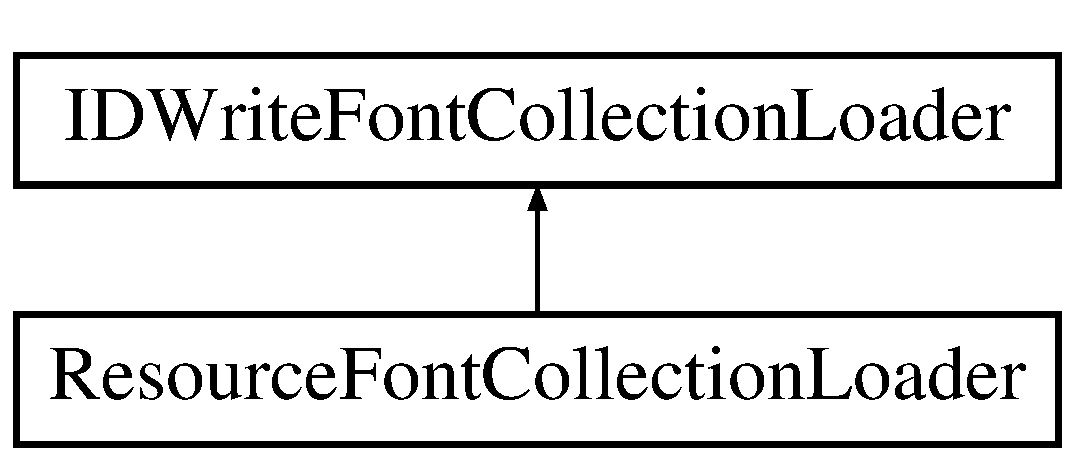
\includegraphics[height=2.000000cm]{class_resource_font_collection_loader}
\end{center}
\end{figure}
\subsection*{Public Member Functions}
\begin{DoxyCompactItemize}
\item 
\hypertarget{class_resource_font_collection_loader_aeb076e9f9989e7bb75e711c321d73a68}{virtual H\-R\-E\-S\-U\-L\-T S\-T\-D\-M\-E\-T\-H\-O\-D\-C\-A\-L\-L\-T\-Y\-P\-E {\bfseries Query\-Interface} (R\-E\-F\-I\-I\-D iid, void $\ast$$\ast$ppv\-Object)}\label{class_resource_font_collection_loader_aeb076e9f9989e7bb75e711c321d73a68}

\item 
\hypertarget{class_resource_font_collection_loader_a2f4562450d74fd66c6d2c529b64b15bd}{virtual U\-L\-O\-N\-G S\-T\-D\-M\-E\-T\-H\-O\-D\-C\-A\-L\-L\-T\-Y\-P\-E {\bfseries Add\-Ref} ()}\label{class_resource_font_collection_loader_a2f4562450d74fd66c6d2c529b64b15bd}

\item 
\hypertarget{class_resource_font_collection_loader_aa5e7a778176b856dc22ea0cd34336818}{virtual U\-L\-O\-N\-G S\-T\-D\-M\-E\-T\-H\-O\-D\-C\-A\-L\-L\-T\-Y\-P\-E {\bfseries Release} ()}\label{class_resource_font_collection_loader_aa5e7a778176b856dc22ea0cd34336818}

\item 
\hypertarget{class_resource_font_collection_loader_a10cf52a851165e73c115a343a3fff727}{virtual H\-R\-E\-S\-U\-L\-T S\-T\-D\-M\-E\-T\-H\-O\-D\-C\-A\-L\-L\-T\-Y\-P\-E {\bfseries Create\-Enumerator\-From\-Key} (I\-D\-Write\-Factory $\ast$factory, void const $\ast$collection\-Key, U\-I\-N\-T32 collection\-Key\-Size, O\-U\-T I\-D\-Write\-Font\-File\-Enumerator $\ast$$\ast$font\-File\-Enumerator)}\label{class_resource_font_collection_loader_a10cf52a851165e73c115a343a3fff727}

\end{DoxyCompactItemize}
\subsection*{Static Public Member Functions}
\begin{DoxyCompactItemize}
\item 
\hypertarget{class_resource_font_collection_loader_a6b7a62a995980bd155b45500f56cf9b4}{static \\*
I\-D\-Write\-Font\-Collection\-Loader $\ast$ {\bfseries Get\-Loader} ()}\label{class_resource_font_collection_loader_a6b7a62a995980bd155b45500f56cf9b4}

\item 
\hypertarget{class_resource_font_collection_loader_a664fd8936c247ff41c015a338b4e72ef}{static bool {\bfseries Is\-Loader\-Initialized} ()}\label{class_resource_font_collection_loader_a664fd8936c247ff41c015a338b4e72ef}

\end{DoxyCompactItemize}


The documentation for this class was generated from the following files\-:\begin{DoxyCompactItemize}
\item 
F\-:/\-S\-V\-N/\-P\-O\-P\-Tools/Resource\-Font\-Collection\-Loader.\-h\item 
F\-:/\-S\-V\-N/\-P\-O\-P\-Tools/Resource\-Font\-Collection\-Loader.\-cpp\end{DoxyCompactItemize}

\hypertarget{class_resource_font_context}{\section{Resource\-Font\-Context Class Reference}
\label{class_resource_font_context}\index{Resource\-Font\-Context@{Resource\-Font\-Context}}
}
\subsection*{Public Member Functions}
\begin{DoxyCompactItemize}
\item 
\hypertarget{class_resource_font_context_abf2e56012e472e0c2d8f81fcd9cced23}{{\bfseries Resource\-Font\-Context} (I\-D\-Write\-Factory $\ast$p\-W\-F)}\label{class_resource_font_context_abf2e56012e472e0c2d8f81fcd9cced23}

\item 
\hypertarget{class_resource_font_context_aa356746f33312645aaf8457701970e8a}{H\-R\-E\-S\-U\-L\-T {\bfseries Initialize} ()}\label{class_resource_font_context_aa356746f33312645aaf8457701970e8a}

\item 
\hypertarget{class_resource_font_context_a38889b18f363c929175706c74315e248}{H\-R\-E\-S\-U\-L\-T {\bfseries Create\-Font\-Collection} (U\-I\-N\-T const $\ast$font\-Collection\-Key, U\-I\-N\-T32 key\-Size, O\-U\-T I\-D\-Write\-Font\-Collection $\ast$$\ast$result)}\label{class_resource_font_context_a38889b18f363c929175706c74315e248}

\end{DoxyCompactItemize}


The documentation for this class was generated from the following files\-:\begin{DoxyCompactItemize}
\item 
F\-:/\-S\-V\-N/\-P\-O\-P\-Tools/Resource\-Font\-Context.\-h\item 
F\-:/\-S\-V\-N/\-P\-O\-P\-Tools/Resource\-Font\-Context.\-cpp\end{DoxyCompactItemize}

\hypertarget{class_resource_font_file_enumerator}{\section{Resource\-Font\-File\-Enumerator Class Reference}
\label{class_resource_font_file_enumerator}\index{Resource\-Font\-File\-Enumerator@{Resource\-Font\-File\-Enumerator}}
}
Inheritance diagram for Resource\-Font\-File\-Enumerator\-:\begin{figure}[H]
\begin{center}
\leavevmode
\includegraphics[height=2.000000cm]{class_resource_font_file_enumerator}
\end{center}
\end{figure}
\subsection*{Public Member Functions}
\begin{DoxyCompactItemize}
\item 
\hypertarget{class_resource_font_file_enumerator_a604ee80befe30fe9f4159ae9c5ecdeea}{{\bfseries Resource\-Font\-File\-Enumerator} (I\-D\-Write\-Factory $\ast$factory)}\label{class_resource_font_file_enumerator_a604ee80befe30fe9f4159ae9c5ecdeea}

\item 
\hypertarget{class_resource_font_file_enumerator_a809072885f8c5ecc23764d57e3b7f0b5}{H\-R\-E\-S\-U\-L\-T {\bfseries Initialize} (U\-I\-N\-T const $\ast$resource\-I\-Ds, U\-I\-N\-T32 resource\-Count)}\label{class_resource_font_file_enumerator_a809072885f8c5ecc23764d57e3b7f0b5}

\item 
\hypertarget{class_resource_font_file_enumerator_a121e0188c536d7324cce24cf1afa0f82}{virtual H\-R\-E\-S\-U\-L\-T S\-T\-D\-M\-E\-T\-H\-O\-D\-C\-A\-L\-L\-T\-Y\-P\-E {\bfseries Query\-Interface} (R\-E\-F\-I\-I\-D iid, void $\ast$$\ast$ppv\-Object)}\label{class_resource_font_file_enumerator_a121e0188c536d7324cce24cf1afa0f82}

\item 
\hypertarget{class_resource_font_file_enumerator_a9410f1c58f02f2d82d549bfe68cf5002}{virtual U\-L\-O\-N\-G S\-T\-D\-M\-E\-T\-H\-O\-D\-C\-A\-L\-L\-T\-Y\-P\-E {\bfseries Add\-Ref} ()}\label{class_resource_font_file_enumerator_a9410f1c58f02f2d82d549bfe68cf5002}

\item 
\hypertarget{class_resource_font_file_enumerator_a67dffdfda8092e36425a9445cc189dfc}{virtual U\-L\-O\-N\-G S\-T\-D\-M\-E\-T\-H\-O\-D\-C\-A\-L\-L\-T\-Y\-P\-E {\bfseries Release} ()}\label{class_resource_font_file_enumerator_a67dffdfda8092e36425a9445cc189dfc}

\item 
\hypertarget{class_resource_font_file_enumerator_ab6b9d3c7e8687186118d238c805ab0f0}{virtual H\-R\-E\-S\-U\-L\-T S\-T\-D\-M\-E\-T\-H\-O\-D\-C\-A\-L\-L\-T\-Y\-P\-E {\bfseries Move\-Next} (O\-U\-T B\-O\-O\-L $\ast$has\-Current\-File)}\label{class_resource_font_file_enumerator_ab6b9d3c7e8687186118d238c805ab0f0}

\item 
\hypertarget{class_resource_font_file_enumerator_a8c7d11daa110300498f7d999b76f2cf2}{virtual H\-R\-E\-S\-U\-L\-T S\-T\-D\-M\-E\-T\-H\-O\-D\-C\-A\-L\-L\-T\-Y\-P\-E {\bfseries Get\-Current\-Font\-File} (O\-U\-T I\-D\-Write\-Font\-File $\ast$$\ast$font\-File)}\label{class_resource_font_file_enumerator_a8c7d11daa110300498f7d999b76f2cf2}

\end{DoxyCompactItemize}


The documentation for this class was generated from the following files\-:\begin{DoxyCompactItemize}
\item 
F\-:/\-S\-V\-N/\-P\-O\-P\-Tools/Resource\-Font\-File\-Enumerator.\-h\item 
F\-:/\-S\-V\-N/\-P\-O\-P\-Tools/Resource\-Font\-File\-Enumerator.\-cpp\end{DoxyCompactItemize}

\hypertarget{class_resource_font_file_loader}{\section{Resource\-Font\-File\-Loader Class Reference}
\label{class_resource_font_file_loader}\index{Resource\-Font\-File\-Loader@{Resource\-Font\-File\-Loader}}
}
Inheritance diagram for Resource\-Font\-File\-Loader\-:\begin{figure}[H]
\begin{center}
\leavevmode
\includegraphics[height=2.000000cm]{class_resource_font_file_loader}
\end{center}
\end{figure}
\subsection*{Public Member Functions}
\begin{DoxyCompactItemize}
\item 
\hypertarget{class_resource_font_file_loader_ac63a6457122ddcca3692af48e2c0855a}{virtual H\-R\-E\-S\-U\-L\-T S\-T\-D\-M\-E\-T\-H\-O\-D\-C\-A\-L\-L\-T\-Y\-P\-E {\bfseries Query\-Interface} (R\-E\-F\-I\-I\-D iid, void $\ast$$\ast$ppv\-Object)}\label{class_resource_font_file_loader_ac63a6457122ddcca3692af48e2c0855a}

\item 
\hypertarget{class_resource_font_file_loader_a45ee198b69c353f36f255042874e0aaa}{virtual U\-L\-O\-N\-G S\-T\-D\-M\-E\-T\-H\-O\-D\-C\-A\-L\-L\-T\-Y\-P\-E {\bfseries Add\-Ref} ()}\label{class_resource_font_file_loader_a45ee198b69c353f36f255042874e0aaa}

\item 
\hypertarget{class_resource_font_file_loader_a9fba78074003205b21cb24d8ebf5adec}{virtual U\-L\-O\-N\-G S\-T\-D\-M\-E\-T\-H\-O\-D\-C\-A\-L\-L\-T\-Y\-P\-E {\bfseries Release} ()}\label{class_resource_font_file_loader_a9fba78074003205b21cb24d8ebf5adec}

\item 
\hypertarget{class_resource_font_file_loader_a024531ae4bd559d252ffbe4c9bbf6147}{virtual H\-R\-E\-S\-U\-L\-T S\-T\-D\-M\-E\-T\-H\-O\-D\-C\-A\-L\-L\-T\-Y\-P\-E {\bfseries Create\-Stream\-From\-Key} (void const $\ast$font\-File\-Reference\-Key, U\-I\-N\-T32 font\-File\-Reference\-Key\-Size, O\-U\-T I\-D\-Write\-Font\-File\-Stream $\ast$$\ast$font\-File\-Stream)}\label{class_resource_font_file_loader_a024531ae4bd559d252ffbe4c9bbf6147}

\end{DoxyCompactItemize}
\subsection*{Static Public Member Functions}
\begin{DoxyCompactItemize}
\item 
\hypertarget{class_resource_font_file_loader_a89a160a1425d040a5699236dfd7d7fdc}{static I\-D\-Write\-Font\-File\-Loader $\ast$ {\bfseries Get\-Loader} ()}\label{class_resource_font_file_loader_a89a160a1425d040a5699236dfd7d7fdc}

\item 
\hypertarget{class_resource_font_file_loader_a24b04152fa11c8dd80bed6a8eaa2cb0b}{static bool {\bfseries Is\-Loader\-Initialized} ()}\label{class_resource_font_file_loader_a24b04152fa11c8dd80bed6a8eaa2cb0b}

\end{DoxyCompactItemize}


The documentation for this class was generated from the following files\-:\begin{DoxyCompactItemize}
\item 
F\-:/\-S\-V\-N/\-P\-O\-P\-Tools/Resource\-Font\-File\-Loader.\-h\item 
F\-:/\-S\-V\-N/\-P\-O\-P\-Tools/Resource\-Font\-File\-Loader.\-cpp\end{DoxyCompactItemize}

\hypertarget{class_resource_font_file_stream}{\section{Resource\-Font\-File\-Stream Class Reference}
\label{class_resource_font_file_stream}\index{Resource\-Font\-File\-Stream@{Resource\-Font\-File\-Stream}}
}
Inheritance diagram for Resource\-Font\-File\-Stream\-:\begin{figure}[H]
\begin{center}
\leavevmode
\includegraphics[height=2.000000cm]{class_resource_font_file_stream}
\end{center}
\end{figure}
\subsection*{Public Member Functions}
\begin{DoxyCompactItemize}
\item 
\hypertarget{class_resource_font_file_stream_a9a5ab096c5ebb91904607f1f5770623a}{{\bfseries Resource\-Font\-File\-Stream} (U\-I\-N\-T resource\-I\-D)}\label{class_resource_font_file_stream_a9a5ab096c5ebb91904607f1f5770623a}

\item 
\hypertarget{class_resource_font_file_stream_aa05f74a3a642894808c75aaf6ed66af6}{virtual H\-R\-E\-S\-U\-L\-T S\-T\-D\-M\-E\-T\-H\-O\-D\-C\-A\-L\-L\-T\-Y\-P\-E {\bfseries Query\-Interface} (R\-E\-F\-I\-I\-D iid, void $\ast$$\ast$ppv\-Object)}\label{class_resource_font_file_stream_aa05f74a3a642894808c75aaf6ed66af6}

\item 
\hypertarget{class_resource_font_file_stream_a39b3b75edab831b285b34a29d5c8f4a6}{virtual U\-L\-O\-N\-G S\-T\-D\-M\-E\-T\-H\-O\-D\-C\-A\-L\-L\-T\-Y\-P\-E {\bfseries Add\-Ref} ()}\label{class_resource_font_file_stream_a39b3b75edab831b285b34a29d5c8f4a6}

\item 
\hypertarget{class_resource_font_file_stream_a963e399b8a36d02d1af29a096021a294}{virtual U\-L\-O\-N\-G S\-T\-D\-M\-E\-T\-H\-O\-D\-C\-A\-L\-L\-T\-Y\-P\-E {\bfseries Release} ()}\label{class_resource_font_file_stream_a963e399b8a36d02d1af29a096021a294}

\item 
\hypertarget{class_resource_font_file_stream_a23d9b9edfdc9fd3adf8ac6f79f71eba8}{virtual H\-R\-E\-S\-U\-L\-T S\-T\-D\-M\-E\-T\-H\-O\-D\-C\-A\-L\-L\-T\-Y\-P\-E {\bfseries Read\-File\-Fragment} (void const $\ast$$\ast$fragment\-Start, U\-I\-N\-T64 file\-Offset, U\-I\-N\-T64 fragment\-Size, O\-U\-T void $\ast$$\ast$fragment\-Context)}\label{class_resource_font_file_stream_a23d9b9edfdc9fd3adf8ac6f79f71eba8}

\item 
\hypertarget{class_resource_font_file_stream_a8f24ef617d76d2d6ae513bd40875c12f}{virtual void S\-T\-D\-M\-E\-T\-H\-O\-D\-C\-A\-L\-L\-T\-Y\-P\-E {\bfseries Release\-File\-Fragment} (void $\ast$fragment\-Context)}\label{class_resource_font_file_stream_a8f24ef617d76d2d6ae513bd40875c12f}

\item 
\hypertarget{class_resource_font_file_stream_a75dbb02d17cface6d956b23121d13118}{virtual H\-R\-E\-S\-U\-L\-T S\-T\-D\-M\-E\-T\-H\-O\-D\-C\-A\-L\-L\-T\-Y\-P\-E {\bfseries Get\-File\-Size} (O\-U\-T U\-I\-N\-T64 $\ast$file\-Size)}\label{class_resource_font_file_stream_a75dbb02d17cface6d956b23121d13118}

\item 
\hypertarget{class_resource_font_file_stream_a6f3a70a76e5bf12030e2dcaf0fdb037c}{virtual H\-R\-E\-S\-U\-L\-T S\-T\-D\-M\-E\-T\-H\-O\-D\-C\-A\-L\-L\-T\-Y\-P\-E {\bfseries Get\-Last\-Write\-Time} (O\-U\-T U\-I\-N\-T64 $\ast$last\-Write\-Time)}\label{class_resource_font_file_stream_a6f3a70a76e5bf12030e2dcaf0fdb037c}

\item 
\hypertarget{class_resource_font_file_stream_a730e4d5e33625e016f5ae57b3ca6553d}{bool {\bfseries Is\-Initialized} ()}\label{class_resource_font_file_stream_a730e4d5e33625e016f5ae57b3ca6553d}

\end{DoxyCompactItemize}


The documentation for this class was generated from the following files\-:\begin{DoxyCompactItemize}
\item 
F\-:/\-S\-V\-N/\-P\-O\-P\-Tools/Resource\-Font\-File\-Stream.\-h\item 
F\-:/\-S\-V\-N/\-P\-O\-P\-Tools/Resource\-Font\-File\-Stream.\-cpp\end{DoxyCompactItemize}

\hypertarget{struct_rotate_list}{\section{Rotate\-List Struct Reference}
\label{struct_rotate_list}\index{Rotate\-List@{Rotate\-List}}
}
\subsection*{Public Attributes}
\begin{DoxyCompactItemize}
\item 
\hypertarget{struct_rotate_list_a52fd4a625dccae1f8cc9ce14e6a7fe5e}{bool {\bfseries clear}}\label{struct_rotate_list_a52fd4a625dccae1f8cc9ce14e6a7fe5e}

\item 
\hypertarget{struct_rotate_list_a3ba0fa27b119cad91efb45324464565a}{unsigned int {\bfseries start}}\label{struct_rotate_list_a3ba0fa27b119cad91efb45324464565a}

\item 
\hypertarget{struct_rotate_list_a35084a23bb8c6edc918448bf7735f841}{unsigned int {\bfseries end}}\label{struct_rotate_list_a35084a23bb8c6edc918448bf7735f841}

\item 
\hypertarget{struct_rotate_list_af9c925950f7c96cbb49ef9ba33eeca23}{struct \hyperlink{struct_rotate_list_item}{Rotate\-List\-Item} {\bfseries items} \mbox{[}R\-O\-T\-A\-T\-E\-L\-I\-S\-T\-\_\-\-S\-I\-Z\-E\mbox{]}}\label{struct_rotate_list_af9c925950f7c96cbb49ef9ba33eeca23}

\end{DoxyCompactItemize}


The documentation for this struct was generated from the following file\-:\begin{DoxyCompactItemize}
\item 
F\-:/\-S\-V\-N/\-P\-O\-P\-Tools/debugdialog.\-cpp\end{DoxyCompactItemize}

\hypertarget{struct_rotate_list_item}{\section{Rotate\-List\-Item Struct Reference}
\label{struct_rotate_list_item}\index{Rotate\-List\-Item@{Rotate\-List\-Item}}
}
\subsection*{Public Attributes}
\begin{DoxyCompactItemize}
\item 
\hypertarget{struct_rotate_list_item_a6b034bd8af0cf224b58a8fb19789f57d}{char {\bfseries txt} \mbox{[}R\-O\-T\-A\-T\-E\-L\-I\-S\-T\-\_\-\-C\-O\-L\-U\-M\-N\-S\mbox{]}\mbox{[}100\mbox{]}}\label{struct_rotate_list_item_a6b034bd8af0cf224b58a8fb19789f57d}

\end{DoxyCompactItemize}


The documentation for this struct was generated from the following file\-:\begin{DoxyCompactItemize}
\item 
F\-:/\-S\-V\-N/\-P\-O\-P\-Tools/debugdialog.\-cpp\end{DoxyCompactItemize}

\hypertarget{struct_settings_tag}{\section{Settings\-Tag Struct Reference}
\label{struct_settings_tag}\index{Settings\-Tag@{Settings\-Tag}}
}
\subsection*{Public Attributes}
\begin{DoxyCompactItemize}
\item 
\hypertarget{struct_settings_tag_a32e099c28c8887f3aad0b8623a87f39a}{int {\bfseries id\-Language}}\label{struct_settings_tag_a32e099c28c8887f3aad0b8623a87f39a}

\item 
\hypertarget{struct_settings_tag_a9b7e35057cd81dfae66531a230d95913}{bool {\bfseries Show\-Simulation\-Warnings}}\label{struct_settings_tag_a9b7e35057cd81dfae66531a230d95913}

\item 
\hypertarget{struct_settings_tag_a1aaef4f8ab448354a47a94c9c3abbe22}{char {\bfseries last\-\_\-search\-\_\-text} \mbox{[}M\-A\-X\-\_\-\-N\-A\-M\-E\-\_\-\-L\-E\-N\mbox{]}}\label{struct_settings_tag_a1aaef4f8ab448354a47a94c9c3abbe22}

\item 
\hypertarget{struct_settings_tag_af95166ddb73be7e89ca26e4a0538e271}{char {\bfseries last\-\_\-new\-\_\-text} \mbox{[}M\-A\-X\-\_\-\-N\-A\-M\-E\-\_\-\-L\-E\-N\mbox{]}}\label{struct_settings_tag_af95166ddb73be7e89ca26e4a0538e271}

\item 
\hypertarget{struct_settings_tag_a35af5abb34c1b3dfc2bc59ff966cb2e8}{char {\bfseries recent\-\_\-list} \mbox{[}M\-A\-X\-\_\-\-R\-E\-C\-E\-N\-T\-\_\-\-I\-T\-E\-M\-S\mbox{]}\mbox{[}M\-A\-X\-\_\-\-P\-A\-T\-H\mbox{]}}\label{struct_settings_tag_a35af5abb34c1b3dfc2bc59ff966cb2e8}

\item 
\hypertarget{struct_settings_tag_a4311cc5ebdea4c4037d3a5f6a0ac1782}{int {\bfseries C\-O\-M\-Port\-Flash}}\label{struct_settings_tag_a4311cc5ebdea4c4037d3a5f6a0ac1782}

\item 
\hypertarget{struct_settings_tag_a929f488648aacb5c51ae2037a4439882}{int {\bfseries C\-O\-M\-Port\-Debug}}\label{struct_settings_tag_a929f488648aacb5c51ae2037a4439882}

\item 
\hypertarget{struct_settings_tag_ab21be9e507245ffbf49818dce9a3c349}{int {\bfseries Auto\-Save\-Interval}}\label{struct_settings_tag_ab21be9e507245ffbf49818dce9a3c349}

\end{DoxyCompactItemize}


The documentation for this struct was generated from the following file\-:\begin{DoxyCompactItemize}
\item 
F\-:/\-S\-V\-N/\-P\-O\-P\-Tools/poptools.\-h\end{DoxyCompactItemize}

\hypertarget{class_s_p_l_a_s_h}{\section{S\-P\-L\-A\-S\-H Class Reference}
\label{class_s_p_l_a_s_h}\index{S\-P\-L\-A\-S\-H@{S\-P\-L\-A\-S\-H}}
}
\subsection*{Public Member Functions}
\begin{DoxyCompactItemize}
\item 
\hypertarget{class_s_p_l_a_s_h_ae76abea4e72dd41ffa9c15a1579513fa}{void {\bfseries Hide} ()}\label{class_s_p_l_a_s_h_ae76abea4e72dd41ffa9c15a1579513fa}

\item 
\hypertarget{class_s_p_l_a_s_h_a517a30018f5e8d99922607768fbd8e5a}{void {\bfseries Show} ()}\label{class_s_p_l_a_s_h_a517a30018f5e8d99922607768fbd8e5a}

\item 
\hypertarget{class_s_p_l_a_s_h_a5ab3e3a61d274b071b862598a535ae7c}{void {\bfseries Init} (H\-W\-N\-D h\-Wnd)}\label{class_s_p_l_a_s_h_a5ab3e3a61d274b071b862598a535ae7c}

\end{DoxyCompactItemize}
\subsection*{Public Attributes}
\begin{DoxyCompactItemize}
\item 
\hypertarget{class_s_p_l_a_s_h_ab3eb1f4b9d1845d16352c3daf691c505}{H\-B\-I\-T\-M\-A\-P {\bfseries h\-Bitmap}}\label{class_s_p_l_a_s_h_ab3eb1f4b9d1845d16352c3daf691c505}

\item 
\hypertarget{class_s_p_l_a_s_h_ae8fd1b18e3b6289d0c65f112e058bb4d}{int {\bfseries tx}}\label{class_s_p_l_a_s_h_ae8fd1b18e3b6289d0c65f112e058bb4d}

\item 
\hypertarget{class_s_p_l_a_s_h_afb62d7de09957ec6bee6fafb804ef91f}{int {\bfseries ty}}\label{class_s_p_l_a_s_h_afb62d7de09957ec6bee6fafb804ef91f}

\item 
\hypertarget{class_s_p_l_a_s_h_aa1e2d3fee453ed4b87eabbf8b4954b58}{int {\bfseries pwidth}}\label{class_s_p_l_a_s_h_aa1e2d3fee453ed4b87eabbf8b4954b58}

\item 
\hypertarget{class_s_p_l_a_s_h_a37518cda0eef4a0f2fdc1b1c0fb08459}{int {\bfseries pheight}}\label{class_s_p_l_a_s_h_a37518cda0eef4a0f2fdc1b1c0fb08459}

\item 
\hypertarget{class_s_p_l_a_s_h_aced601d0773a97ebc35fd0add43e0c75}{B\-O\-O\-L {\bfseries S\-H\-O\-W\-I\-N\-G}}\label{class_s_p_l_a_s_h_aced601d0773a97ebc35fd0add43e0c75}

\end{DoxyCompactItemize}


The documentation for this class was generated from the following files\-:\begin{DoxyCompactItemize}
\item 
F\-:/\-S\-V\-N/\-P\-O\-P\-Tools/splash.\-h\item 
F\-:/\-S\-V\-N/\-P\-O\-P\-Tools/splash.\-cpp\end{DoxyCompactItemize}

\hypertarget{structstr_cmd_state_list}{\section{str\-Cmd\-State\-List Struct Reference}
\label{structstr_cmd_state_list}\index{str\-Cmd\-State\-List@{str\-Cmd\-State\-List}}
}
\subsection*{Public Attributes}
\begin{DoxyCompactItemize}
\item 
\hypertarget{structstr_cmd_state_list_a1ee146cf64c9a75df8ffdc2b7b784c9e}{U\-I\-N\-T {\bfseries u\-Cmd\-I\-D}}\label{structstr_cmd_state_list_a1ee146cf64c9a75df8ffdc2b7b784c9e}

\item 
\hypertarget{structstr_cmd_state_list_ae3aeec8a299d3e1f7a170a30f451f587}{B\-O\-O\-L {\bfseries state}}\label{structstr_cmd_state_list_ae3aeec8a299d3e1f7a170a30f451f587}

\item 
\hypertarget{structstr_cmd_state_list_a8914e85c5f5d8c09c2b81b56d6ebb36b}{struct \hyperlink{structstr_cmd_state_list}{str\-Cmd\-State\-List} $\ast$ {\bfseries next}}\label{structstr_cmd_state_list_a8914e85c5f5d8c09c2b81b56d6ebb36b}

\end{DoxyCompactItemize}


The documentation for this struct was generated from the following file\-:\begin{DoxyCompactItemize}
\item 
F\-:/\-S\-V\-N/\-P\-O\-P\-Tools/Ribbon.\-cpp\end{DoxyCompactItemize}

\hypertarget{structstr_hardware_registers}{\section{str\-Hardware\-Registers Struct Reference}
\label{structstr_hardware_registers}\index{str\-Hardware\-Registers@{str\-Hardware\-Registers}}
}
\subsection*{Public Attributes}
\begin{DoxyCompactItemize}
\item 
\hypertarget{structstr_hardware_registers_a0e290696b1019bc85756ebd675c6ddb5}{unsigned int {\bfseries Digital\-Input}}\label{structstr_hardware_registers_a0e290696b1019bc85756ebd675c6ddb5}

\item 
\hypertarget{structstr_hardware_registers_a5b22556d98c96e850e668aada52f2b65}{unsigned int {\bfseries Digital\-Output}}\label{structstr_hardware_registers_a5b22556d98c96e850e668aada52f2b65}

\item 
\hypertarget{structstr_hardware_registers_a48867e1f43e7841783d860932d0a6090}{int {\bfseries Mod\-B\-U\-S} \mbox{[}H\-W\-R\-\_\-\-M\-O\-D\-B\-U\-S\-\_\-\-S\-I\-Z\-E\mbox{]}}\label{structstr_hardware_registers_a48867e1f43e7841783d860932d0a6090}

\item 
\hypertarget{structstr_hardware_registers_a27d20a3ab139cbf4c6819c38482671a5}{bool {\bfseries Syncing}}\label{structstr_hardware_registers_a27d20a3ab139cbf4c6819c38482671a5}

\item 
\hypertarget{structstr_hardware_registers_a7b5e8fc07658b6e83b6e0334c97ea1a9}{bool {\bfseries Need\-Update}}\label{structstr_hardware_registers_a7b5e8fc07658b6e83b6e0334c97ea1a9}

\end{DoxyCompactItemize}


The documentation for this struct was generated from the following file\-:\begin{DoxyCompactItemize}
\item 
F\-:/\-S\-V\-N/\-P\-O\-P\-Tools/poptools.\-h\end{DoxyCompactItemize}

\hypertarget{structstr_serial_config}{\section{str\-Serial\-Config Struct Reference}
\label{structstr_serial_config}\index{str\-Serial\-Config@{str\-Serial\-Config}}
}
\subsection*{Public Attributes}
\begin{DoxyCompactItemize}
\item 
\hypertarget{structstr_serial_config_aa6d4be7e69575af7e1359f50d5a66645}{B\-Y\-T\-E {\bfseries b\-Byte\-Size}}\label{structstr_serial_config_aa6d4be7e69575af7e1359f50d5a66645}

\item 
\hypertarget{structstr_serial_config_af5ddcf2090cb8712b1c7949f012973a6}{B\-Y\-T\-E {\bfseries b\-Parity}}\label{structstr_serial_config_af5ddcf2090cb8712b1c7949f012973a6}

\item 
\hypertarget{structstr_serial_config_a221e833b05d0a28134c4df46ee77afba}{B\-Y\-T\-E {\bfseries b\-Stop\-Bits}}\label{structstr_serial_config_a221e833b05d0a28134c4df46ee77afba}

\item 
\hypertarget{structstr_serial_config_aa588953fc89297ab0e82615e040ea7d1}{char $\ast$ {\bfseries Config\-Name}}\label{structstr_serial_config_aa588953fc89297ab0e82615e040ea7d1}

\end{DoxyCompactItemize}


The documentation for this struct was generated from the following file\-:\begin{DoxyCompactItemize}
\item 
F\-:/\-S\-V\-N/\-P\-O\-P\-Tools/poptools.\-h\end{DoxyCompactItemize}

\hypertarget{struct_subckt}{\section{Subckt Struct Reference}
\label{struct_subckt}\index{Subckt@{Subckt}}
}
\subsection*{Public Attributes}
\begin{DoxyCompactItemize}
\item 
\hypertarget{struct_subckt_a3e1dea91acbcc8625dccd8cf573543d1}{\hyperlink{class_ladder_elem}{Ladder\-Elem} $\ast$ {\bfseries elem}}\label{struct_subckt_a3e1dea91acbcc8625dccd8cf573543d1}

\item 
\hypertarget{struct_subckt_a824a86a9713c4570df8fc560eb7317b8}{\hyperlink{class_ladder_circuit}{Ladder\-Circuit} $\ast$ {\bfseries subckt}}\label{struct_subckt_a824a86a9713c4570df8fc560eb7317b8}

\end{DoxyCompactItemize}


The documentation for this struct was generated from the following file\-:\begin{DoxyCompactItemize}
\item 
F\-:/\-S\-V\-N/\-P\-O\-P\-Tools/Ladder\-Objects.\-h\end{DoxyCompactItemize}

\hypertarget{structt_brush_data_d2_d}{\section{t\-Brush\-Data\-D2\-D Struct Reference}
\label{structt_brush_data_d2_d}\index{t\-Brush\-Data\-D2\-D@{t\-Brush\-Data\-D2\-D}}
}
\subsection*{Public Attributes}
\begin{DoxyCompactItemize}
\item 
\hypertarget{structt_brush_data_d2_d_a54d3d09db4849518f3405cb03039b87c}{e\-Brush\-Type {\bfseries brush\-Type}}\label{structt_brush_data_d2_d_a54d3d09db4849518f3405cb03039b87c}

\item 
\hypertarget{structt_brush_data_d2_d_a53f2c9a053a5c8240df60f69793b365d}{\begin{tabbing}
xx\=xx\=xx\=xx\=xx\=xx\=xx\=xx\=xx\=\kill
struct \{\\
\>ID2D1SolidColorBrush $\ast$ {\bfseries pBrush}\\
\} {\bfseries solid}}\label{structt_brush_data_d2_d_a53f2c9a053a5c8240df60f69793b365d}
\\

\end{tabbing}\item 
\hypertarget{structt_brush_data_d2_d_a1bcd580c1b1ecc18467bfeff532d74ba}{\begin{tabbing}
xx\=xx\=xx\=xx\=xx\=xx\=xx\=xx\=xx\=\kill
struct \{\\
\>unsigned int {\bfseries angle}\\
\>ID2D1LinearGradientBrush $\ast$ {\bfseries pBrush}\\
\>ID2D1GradientStopCollection $\ast$ {\bfseries pGradientStops}\\
\} {\bfseries linear}}\label{structt_brush_data_d2_d_a1bcd580c1b1ecc18467bfeff532d74ba}
\\

\end{tabbing}\end{DoxyCompactItemize}


The documentation for this struct was generated from the following file\-:\begin{DoxyCompactItemize}
\item 
F\-:/\-S\-V\-N/\-P\-O\-P\-Tools/Engine\-Render\-D2\-D.\-h\end{DoxyCompactItemize}

\hypertarget{structt_cmd_change_name_data}{\section{t\-Cmd\-Change\-Name\-Data Struct Reference}
\label{structt_cmd_change_name_data}\index{t\-Cmd\-Change\-Name\-Data@{t\-Cmd\-Change\-Name\-Data}}
}
\subsection*{Public Attributes}
\begin{DoxyCompactItemize}
\item 
\hypertarget{structt_cmd_change_name_data_a5c82b2a5f4834abb9b1be12c1f403e8c}{e\-Type {\bfseries type}}\label{structt_cmd_change_name_data_a5c82b2a5f4834abb9b1be12c1f403e8c}

\item 
\hypertarget{structt_cmd_change_name_data_a40d2aedb764d8faee953044e53114e06}{bool {\bfseries reply}}\label{structt_cmd_change_name_data_a40d2aedb764d8faee953044e53114e06}

\end{DoxyCompactItemize}


The documentation for this struct was generated from the following file\-:\begin{DoxyCompactItemize}
\item 
F\-:/\-S\-V\-N/\-P\-O\-P\-Tools/Ladder\-G\-U\-I.\-h\end{DoxyCompactItemize}

\hypertarget{structt_cmd_expanded_item}{\section{t\-Cmd\-Expanded\-Item Struct Reference}
\label{structt_cmd_expanded_item}\index{t\-Cmd\-Expanded\-Item@{t\-Cmd\-Expanded\-Item}}
}
\subsection*{Public Attributes}
\begin{DoxyCompactItemize}
\item 
\hypertarget{structt_cmd_expanded_item_a7ac5a59e0fb754044367f1c3cb3571e5}{t\-Fnc\-Expanded\-Item {\bfseries fnc}}\label{structt_cmd_expanded_item_a7ac5a59e0fb754044367f1c3cb3571e5}

\item 
\hypertarget{structt_cmd_expanded_item_a5a75196b7b3b685754f0f188587b67b7}{unsigned int {\bfseries index}}\label{structt_cmd_expanded_item_a5a75196b7b3b685754f0f188587b67b7}

\end{DoxyCompactItemize}


The documentation for this struct was generated from the following file\-:\begin{DoxyCompactItemize}
\item 
F\-:/\-S\-V\-N/\-P\-O\-P\-Tools/Ladder\-G\-U\-I.\-h\end{DoxyCompactItemize}

\hypertarget{structt_command_source}{\section{t\-Command\-Source Struct Reference}
\label{structt_command_source}\index{t\-Command\-Source@{t\-Command\-Source}}
}
\subsection*{Public Attributes}
\begin{DoxyCompactItemize}
\item 
\hypertarget{structt_command_source_a335e2b480fb4978949f9d39ed437b752}{\hyperlink{class_ladder_diagram}{Ladder\-Diagram} $\ast$ {\bfseries diagram}}\label{structt_command_source_a335e2b480fb4978949f9d39ed437b752}

\item 
\hypertarget{structt_command_source_a78199af7eba9e684190fbe14be975fcc}{\hyperlink{class_ladder_circuit}{Ladder\-Circuit} $\ast$ {\bfseries circuit}}\label{structt_command_source_a78199af7eba9e684190fbe14be975fcc}

\item 
\hypertarget{structt_command_source_ab3a4d7985bfc5edb8b9fa2a3e39f83c7}{\hyperlink{class_ladder_elem}{Ladder\-Elem} $\ast$ {\bfseries elem}}\label{structt_command_source_ab3a4d7985bfc5edb8b9fa2a3e39f83c7}

\end{DoxyCompactItemize}


The documentation for this struct was generated from the following file\-:\begin{DoxyCompactItemize}
\item 
F\-:/\-S\-V\-N/\-P\-O\-P\-Tools/Ladder\-G\-U\-I.\-h\end{DoxyCompactItemize}

\hypertarget{structt_connection_dot}{\section{t\-Connection\-Dot Struct Reference}
\label{structt_connection_dot}\index{t\-Connection\-Dot@{t\-Connection\-Dot}}
}
\subsection*{Public Attributes}
\begin{DoxyCompactItemize}
\item 
\hypertarget{structt_connection_dot_a244f9d12a670cd0bb95bfaa0ff58f4f1}{P\-O\-I\-N\-T {\bfseries dot}}\label{structt_connection_dot_a244f9d12a670cd0bb95bfaa0ff58f4f1}

\item 
\hypertarget{structt_connection_dot_ab362928f44954b46288b224b6f89aff3}{unsigned int {\bfseries count}}\label{structt_connection_dot_ab362928f44954b46288b224b6f89aff3}

\item 
\hypertarget{structt_connection_dot_a144ce7d7fcf035a4f40265c7225aa4e2}{bool {\bfseries is\-Powered}}\label{structt_connection_dot_a144ce7d7fcf035a4f40265c7225aa4e2}

\end{DoxyCompactItemize}


The documentation for this struct was generated from the following file\-:\begin{DoxyCompactItemize}
\item 
F\-:/\-S\-V\-N/\-P\-O\-P\-Tools/Ladder\-G\-U\-I.\-h\end{DoxyCompactItemize}

\hypertarget{structt_control_list}{\section{t\-Control\-List Struct Reference}
\label{structt_control_list}\index{t\-Control\-List@{t\-Control\-List}}
}
\subsection*{Public Attributes}
\begin{DoxyCompactItemize}
\item 
\hypertarget{structt_control_list_a0a474e5e979109230fd929693e900a5f}{t\-Fnc\-Expanded\-Item {\bfseries fnc}}\label{structt_control_list_a0a474e5e979109230fd929693e900a5f}

\item 
\hypertarget{structt_control_list_adacc0d1e65e0c534f850320422e4b75d}{vector$<$ string $>$ {\bfseries items}}\label{structt_control_list_adacc0d1e65e0c534f850320422e4b75d}

\item 
\hypertarget{structt_control_list_ae9d8f2170294e773f29b3062c609a718}{int {\bfseries selected}}\label{structt_control_list_ae9d8f2170294e773f29b3062c609a718}

\end{DoxyCompactItemize}


The documentation for this struct was generated from the following file\-:\begin{DoxyCompactItemize}
\item 
F\-:/\-S\-V\-N/\-P\-O\-P\-Tools/Ladder\-G\-U\-I.\-h\end{DoxyCompactItemize}

\hypertarget{structt_conv_string}{\section{t\-Conv\-String Struct Reference}
\label{structt_conv_string}\index{t\-Conv\-String@{t\-Conv\-String}}
}
\subsection*{Public Attributes}
\begin{DoxyCompactItemize}
\item 
\hypertarget{structt_conv_string_aea4bd2e820673103e44d269bd8aa6d3c}{bool {\bfseries Char\-To\-Wide\-Char}}\label{structt_conv_string_aea4bd2e820673103e44d269bd8aa6d3c}

\item 
\hypertarget{structt_conv_string_ae63aeff761511a2a640ff27993c276ed}{char $\ast$ {\bfseries p\-Char}}\label{structt_conv_string_ae63aeff761511a2a640ff27993c276ed}

\item 
\hypertarget{structt_conv_string_a1761779ffcdd623333296f81a4ac9e61}{wchar\-\_\-t $\ast$ {\bfseries p\-Wide\-Char}}\label{structt_conv_string_a1761779ffcdd623333296f81a4ac9e61}

\end{DoxyCompactItemize}


The documentation for this struct was generated from the following file\-:\begin{DoxyCompactItemize}
\item 
F\-:/\-S\-V\-N/\-P\-O\-P\-Tools/poptools.\-h\end{DoxyCompactItemize}

\hypertarget{structt_data_draw_g_u_i}{\section{t\-Data\-Draw\-G\-U\-I Struct Reference}
\label{structt_data_draw_g_u_i}\index{t\-Data\-Draw\-G\-U\-I@{t\-Data\-Draw\-G\-U\-I}}
}
\subsection*{Public Attributes}
\begin{DoxyCompactItemize}
\item 
\hypertarget{structt_data_draw_g_u_i_a12abe156d9b5babc16d5b4c1c8c21c04}{P\-O\-I\-N\-T {\bfseries start}}\label{structt_data_draw_g_u_i_a12abe156d9b5babc16d5b4c1c8c21c04}

\item 
\hypertarget{structt_data_draw_g_u_i_a882b89a0d537c78e55b010bcc173fb35}{P\-O\-I\-N\-T {\bfseries size}}\label{structt_data_draw_g_u_i_a882b89a0d537c78e55b010bcc173fb35}

\item 
\hypertarget{structt_data_draw_g_u_i_aedc8b19fb0bc9815414f2f880dd95909}{R\-E\-C\-T {\bfseries region}}\label{structt_data_draw_g_u_i_aedc8b19fb0bc9815414f2f880dd95909}

\item 
\hypertarget{structt_data_draw_g_u_i_a8e508544a1cd3d208e5b29887d99bc8a}{R\-E\-C\-T {\bfseries region\-Selected}}\label{structt_data_draw_g_u_i_a8e508544a1cd3d208e5b29887d99bc8a}

\item 
\hypertarget{structt_data_draw_g_u_i_ad8569def2b8458cb616ead418ad13eb1}{bool {\bfseries expanded}}\label{structt_data_draw_g_u_i_ad8569def2b8458cb616ead418ad13eb1}

\item 
\hypertarget{structt_data_draw_g_u_i_aa55b0f6fc75dd5a8a0128495ee2d23b2}{bool {\bfseries Dont\-Draw}}\label{structt_data_draw_g_u_i_aa55b0f6fc75dd5a8a0128495ee2d23b2}

\item 
\hypertarget{structt_data_draw_g_u_i_aaef01b9fd5718ef620b5327d6a1a2a64}{bool {\bfseries is\-Full\-Redraw}}\label{structt_data_draw_g_u_i_aaef01b9fd5718ef620b5327d6a1a2a64}

\item 
\hypertarget{structt_data_draw_g_u_i_a8ff6f81476541b13ca05876a7fe4ec5e}{bool {\bfseries has\-Breakpoint}}\label{structt_data_draw_g_u_i_a8ff6f81476541b13ca05876a7fe4ec5e}

\item 
\hypertarget{structt_data_draw_g_u_i_ad5761bd44604dad30308fb10fba8c4a0}{bool {\bfseries is\-Breakpoint\-Active}}\label{structt_data_draw_g_u_i_ad5761bd44604dad30308fb10fba8c4a0}

\item 
\hypertarget{structt_data_draw_g_u_i_ac7fff636ab1def5fc5187d9fac3b3854}{\hyperlink{struct_ladder_context}{Ladder\-Context} $\ast$ {\bfseries context}}\label{structt_data_draw_g_u_i_ac7fff636ab1def5fc5187d9fac3b3854}

\end{DoxyCompactItemize}


The documentation for this struct was generated from the following file\-:\begin{DoxyCompactItemize}
\item 
F\-:/\-S\-V\-N/\-P\-O\-P\-Tools/Ladder\-G\-U\-I.\-h\end{DoxyCompactItemize}

\hypertarget{structt_diagram_data}{\section{t\-Diagram\-Data Struct Reference}
\label{structt_diagram_data}\index{t\-Diagram\-Data@{t\-Diagram\-Data}}
}
\subsection*{Public Attributes}
\begin{DoxyCompactItemize}
\item 
\hypertarget{structt_diagram_data_a839e5db4507a397585104f9b55ab458e}{P\-O\-I\-N\-T {\bfseries Size\-Max}}\label{structt_diagram_data_a839e5db4507a397585104f9b55ab458e}

\item 
\hypertarget{structt_diagram_data_a5101f8e25333a8147adc3f6e4015ab8a}{P\-O\-I\-N\-T {\bfseries Scroll\-Offset}}\label{structt_diagram_data_a5101f8e25333a8147adc3f6e4015ab8a}

\item 
\hypertarget{structt_diagram_data_aa8d29be3065552164ebd8f72dc8ac0cf}{vector$<$ \hyperlink{structt_data_draw_g_u_i}{t\-Data\-Draw\-G\-U\-I} $>$ {\bfseries rung\-Data}}\label{structt_diagram_data_aa8d29be3065552164ebd8f72dc8ac0cf}

\item 
\hypertarget{structt_diagram_data_a39a177a1113c19363b6e0dd9411caf67}{bool {\bfseries need\-Select\-Rung}}\label{structt_diagram_data_a39a177a1113c19363b6e0dd9411caf67}

\end{DoxyCompactItemize}


The documentation for this struct was generated from the following file\-:\begin{DoxyCompactItemize}
\item 
F\-:/\-S\-V\-N/\-P\-O\-P\-Tools/Ladder\-G\-U\-I.\-h\end{DoxyCompactItemize}

\hypertarget{structt_dialog_data}{\section{t\-Dialog\-Data Struct Reference}
\label{structt_dialog_data}\index{t\-Dialog\-Data@{t\-Dialog\-Data}}
}
\subsection*{Public Attributes}
\begin{DoxyCompactItemize}
\item 
\hypertarget{structt_dialog_data_a08d2e92a09d11a1da923d461ae34115a}{e\-Dialog\-Type {\bfseries type}}\label{structt_dialog_data_a08d2e92a09d11a1da923d461ae34115a}

\item 
\hypertarget{structt_dialog_data_ac3034571791921cfdbe5c08b3708c1ad}{bool {\bfseries has\-Cancel}}\label{structt_dialog_data_ac3034571791921cfdbe5c08b3708c1ad}

\item 
\hypertarget{structt_dialog_data_a14df63b3b1358f7e12df8425b681c81f}{e\-Reply $\ast$ {\bfseries reply}}\label{structt_dialog_data_a14df63b3b1358f7e12df8425b681c81f}

\item 
\hypertarget{structt_dialog_data_af5cee56a7ff8cf6d34e9ccf707667116}{string {\bfseries title}}\label{structt_dialog_data_af5cee56a7ff8cf6d34e9ccf707667116}

\item 
\hypertarget{structt_dialog_data_ab6e5ad7f735059f85b8fdeb7abb111c2}{string {\bfseries message}}\label{structt_dialog_data_ab6e5ad7f735059f85b8fdeb7abb111c2}

\end{DoxyCompactItemize}


The documentation for this struct was generated from the following file\-:\begin{DoxyCompactItemize}
\item 
F\-:/\-S\-V\-N/\-P\-O\-P\-Tools/Ladder\-G\-U\-I.\-h\end{DoxyCompactItemize}

\hypertarget{structt_ladder_color_group}{\section{t\-Ladder\-Color\-Group Struct Reference}
\label{structt_ladder_color_group}\index{t\-Ladder\-Color\-Group@{t\-Ladder\-Color\-Group}}
}
\subsection*{Public Attributes}
\begin{DoxyCompactItemize}
\item 
\hypertarget{structt_ladder_color_group_ab8dcb7e1f6a87a1ab3267d4eb4ea368c}{C\-O\-L\-O\-R\-R\-E\-F {\bfseries Background}}\label{structt_ladder_color_group_ab8dcb7e1f6a87a1ab3267d4eb4ea368c}

\item 
\hypertarget{structt_ladder_color_group_ab915d77e180e0b3de26aa5f4d4f890d9}{C\-O\-L\-O\-R\-R\-E\-F {\bfseries Foreground}}\label{structt_ladder_color_group_ab915d77e180e0b3de26aa5f4d4f890d9}

\item 
\hypertarget{structt_ladder_color_group_a9e8a87850780196f50ee1b34b7728594}{C\-O\-L\-O\-R\-R\-E\-F {\bfseries Border}}\label{structt_ladder_color_group_a9e8a87850780196f50ee1b34b7728594}

\item 
\hypertarget{structt_ladder_color_group_a7f0af5b2d0f4b87cb32bc2d48e1eb42c}{C\-O\-L\-O\-R\-R\-E\-F {\bfseries Border\-Text}}\label{structt_ladder_color_group_a7f0af5b2d0f4b87cb32bc2d48e1eb42c}

\end{DoxyCompactItemize}


The documentation for this struct was generated from the following file\-:\begin{DoxyCompactItemize}
\item 
F\-:/\-S\-V\-N/\-P\-O\-P\-Tools/Ladder\-G\-U\-I.\-h\end{DoxyCompactItemize}

\hypertarget{structt_ladder_colors}{\section{t\-Ladder\-Colors Struct Reference}
\label{structt_ladder_colors}\index{t\-Ladder\-Colors@{t\-Ladder\-Colors}}
}
\subsection*{Public Attributes}
\begin{DoxyCompactItemize}
\item 
\hypertarget{structt_ladder_colors_aba2451c1474eb83146440b18c5467a39}{C\-O\-L\-O\-R\-R\-E\-F {\bfseries Background}}\label{structt_ladder_colors_aba2451c1474eb83146440b18c5467a39}

\item 
\hypertarget{structt_ladder_colors_af078bee47d8f1b7ab9f2de78e81b392d}{C\-O\-L\-O\-R\-R\-E\-F {\bfseries Foreground}}\label{structt_ladder_colors_af078bee47d8f1b7ab9f2de78e81b392d}

\item 
\hypertarget{structt_ladder_colors_a51a15ee4ca7e3100f67f405d7f9805ce}{C\-O\-L\-O\-R\-R\-E\-F {\bfseries Bus}}\label{structt_ladder_colors_a51a15ee4ca7e3100f67f405d7f9805ce}

\item 
\hypertarget{structt_ladder_colors_a33f2f3e8a38627ebdb8be8ebe0eb6db5}{C\-O\-L\-O\-R\-R\-E\-F {\bfseries Bus\-Off}}\label{structt_ladder_colors_a33f2f3e8a38627ebdb8be8ebe0eb6db5}

\item 
\hypertarget{structt_ladder_colors_aa52e5cac0a792263a854ffa1d85947c3}{C\-O\-L\-O\-R\-R\-E\-F {\bfseries Wire}}\label{structt_ladder_colors_aa52e5cac0a792263a854ffa1d85947c3}

\item 
\hypertarget{structt_ladder_colors_a9e3c3988e5b3be96f6aa4f4b8dc0623b}{C\-O\-L\-O\-R\-R\-E\-F {\bfseries Wire\-Off}}\label{structt_ladder_colors_a9e3c3988e5b3be96f6aa4f4b8dc0623b}

\item 
\hypertarget{structt_ladder_colors_ab59354a616d8a8722b99ef8d4b8c2b69}{C\-O\-L\-O\-R\-R\-E\-F {\bfseries Selection}}\label{structt_ladder_colors_ab59354a616d8a8722b99ef8d4b8c2b69}

\item 
\hypertarget{structt_ladder_colors_a98a2512b20d65d41264e09eb409ebdb4}{C\-O\-L\-O\-R\-R\-E\-F {\bfseries Breakpoint}}\label{structt_ladder_colors_a98a2512b20d65d41264e09eb409ebdb4}

\item 
\hypertarget{structt_ladder_colors_a4110231e4369b2158478fd23f1fafcb5}{C\-O\-L\-O\-R\-R\-E\-F {\bfseries Connection\-Dot}}\label{structt_ladder_colors_a4110231e4369b2158478fd23f1fafcb5}

\item 
\hypertarget{structt_ladder_colors_a0952d6dbc030de3d780d7f0368a99767}{C\-O\-L\-O\-R\-R\-E\-F {\bfseries Connection\-Dot\-Off}}\label{structt_ladder_colors_a0952d6dbc030de3d780d7f0368a99767}

\item 
\hypertarget{structt_ladder_colors_a15ce9d8e7592d3c5acf134dad54d6e85}{C\-O\-L\-O\-R\-R\-E\-F {\bfseries White}}\label{structt_ladder_colors_a15ce9d8e7592d3c5acf134dad54d6e85}

\item 
\hypertarget{structt_ladder_colors_a93812f4c2ee562b8d14632bb65eb2ac9}{C\-O\-L\-O\-R\-R\-E\-F {\bfseries Black}}\label{structt_ladder_colors_a93812f4c2ee562b8d14632bb65eb2ac9}

\item 
\hypertarget{structt_ladder_colors_ab03212ccb90dc35ff60074c1583abba2}{C\-O\-L\-O\-R\-R\-E\-F {\bfseries Red}}\label{structt_ladder_colors_ab03212ccb90dc35ff60074c1583abba2}

\item 
\hypertarget{structt_ladder_colors_a51f5545c4ef0324732c2b8b60c6b4a68}{C\-O\-L\-O\-R\-R\-E\-F {\bfseries Green}}\label{structt_ladder_colors_a51f5545c4ef0324732c2b8b60c6b4a68}

\item 
\hypertarget{structt_ladder_colors_ab365b33d1ea7ffbc30bd238e04e24163}{C\-O\-L\-O\-R\-R\-E\-F {\bfseries Blue}}\label{structt_ladder_colors_ab365b33d1ea7ffbc30bd238e04e24163}

\item 
\hypertarget{structt_ladder_colors_a7e7c0feb58378c51a924654710c154e1}{C\-O\-L\-O\-R\-R\-E\-F {\bfseries Dialog\-Border}}\label{structt_ladder_colors_a7e7c0feb58378c51a924654710c154e1}

\item 
\hypertarget{structt_ladder_colors_aba40842433615bb6290779b5a580a14e}{C\-O\-L\-O\-R\-R\-E\-F {\bfseries Dialog\-Border\-Text}}\label{structt_ladder_colors_aba40842433615bb6290779b5a580a14e}

\item 
\hypertarget{structt_ladder_colors_ac66946aa4248860469f7dcb71ed5a0e2}{C\-O\-L\-O\-R\-R\-E\-F {\bfseries Dialog\-Background}}\label{structt_ladder_colors_ac66946aa4248860469f7dcb71ed5a0e2}

\item 
\hypertarget{structt_ladder_colors_ac45a158d282565a97ca76da1de699ab6}{C\-O\-L\-O\-R\-R\-E\-F {\bfseries Dialog\-Background\-Light}}\label{structt_ladder_colors_ac45a158d282565a97ca76da1de699ab6}

\item 
\hypertarget{structt_ladder_colors_a5485ca149694318067e148ff612ea52f}{C\-O\-L\-O\-R\-R\-E\-F {\bfseries Dialog\-Background\-Dark}}\label{structt_ladder_colors_a5485ca149694318067e148ff612ea52f}

\item 
\hypertarget{structt_ladder_colors_ad9cdea0b73684dafdb7a435b519f4b86}{C\-O\-L\-O\-R\-R\-E\-F {\bfseries Dialog\-Background\-Text}}\label{structt_ladder_colors_ad9cdea0b73684dafdb7a435b519f4b86}

\item 
\hypertarget{structt_ladder_colors_a1b9c1f65a4b0a1dd893d33c0fe79c200}{C\-O\-L\-O\-R\-R\-E\-F {\bfseries Dialog\-Def\-Button\-Up}}\label{structt_ladder_colors_a1b9c1f65a4b0a1dd893d33c0fe79c200}

\item 
\hypertarget{structt_ladder_colors_a155e68456d1092841561243053880c3f}{C\-O\-L\-O\-R\-R\-E\-F {\bfseries Dialog\-Def\-Button\-Down}}\label{structt_ladder_colors_a155e68456d1092841561243053880c3f}

\item 
\hypertarget{structt_ladder_colors_a83abebd5c080bf6156806ab96764dc35}{C\-O\-L\-O\-R\-R\-E\-F {\bfseries Dialog\-Def\-Button\-Border}}\label{structt_ladder_colors_a83abebd5c080bf6156806ab96764dc35}

\item 
\hypertarget{structt_ladder_colors_ad2535dac59685934f5648b2989326e59}{C\-O\-L\-O\-R\-R\-E\-F {\bfseries Dialog\-Def\-Button\-Text}}\label{structt_ladder_colors_ad2535dac59685934f5648b2989326e59}

\item 
\hypertarget{structt_ladder_colors_aaadb721418d729c09b73e360ad1aa2a6}{C\-O\-L\-O\-R\-R\-E\-F {\bfseries Dialog\-Button\-Up}}\label{structt_ladder_colors_aaadb721418d729c09b73e360ad1aa2a6}

\item 
\hypertarget{structt_ladder_colors_a1cdee729d84b4e53a2b91c880c70f268}{C\-O\-L\-O\-R\-R\-E\-F {\bfseries Dialog\-Button\-Down}}\label{structt_ladder_colors_a1cdee729d84b4e53a2b91c880c70f268}

\item 
\hypertarget{structt_ladder_colors_add5c778cdd99fd12d56e04065d6de05b}{C\-O\-L\-O\-R\-R\-E\-F {\bfseries Dialog\-Button\-Border}}\label{structt_ladder_colors_add5c778cdd99fd12d56e04065d6de05b}

\item 
\hypertarget{structt_ladder_colors_aabb1c4bdf3a464fd84006961286d6412}{C\-O\-L\-O\-R\-R\-E\-F {\bfseries Dialog\-Button\-Text}}\label{structt_ladder_colors_aabb1c4bdf3a464fd84006961286d6412}

\item 
\hypertarget{structt_ladder_colors_a142c090dea9ebfd17c88559ac025de03}{C\-O\-L\-O\-R\-R\-E\-F {\bfseries Black\-Half\-Transparency}}\label{structt_ladder_colors_a142c090dea9ebfd17c88559ac025de03}

\end{DoxyCompactItemize}


The documentation for this struct was generated from the following file\-:\begin{DoxyCompactItemize}
\item 
F\-:/\-S\-V\-N/\-P\-O\-P\-Tools/Ladder\-G\-U\-I.\-h\end{DoxyCompactItemize}

\hypertarget{structt_log_ref_i_o}{\section{t\-Log\-Ref\-I\-O Struct Reference}
\label{structt_log_ref_i_o}\index{t\-Log\-Ref\-I\-O@{t\-Log\-Ref\-I\-O}}
}
\subsection*{Public Attributes}
\begin{DoxyCompactItemize}
\item 
\hypertarget{structt_log_ref_i_o_a54308bb5d6b9828099a1bd93240d313f}{bool {\bfseries is\-Bit}}\label{structt_log_ref_i_o_a54308bb5d6b9828099a1bd93240d313f}

\item 
\hypertarget{structt_log_ref_i_o_a4f4583a63346e2b66428ef9cd71d68aa}{bool {\bfseries is\-Pending}}\label{structt_log_ref_i_o_a4f4583a63346e2b66428ef9cd71d68aa}

\item 
\hypertarget{structt_log_ref_i_o_afe766343ce4aad9b9a288b132d63835b}{string {\bfseries name}}\label{structt_log_ref_i_o_afe766343ce4aad9b9a288b132d63835b}

\item 
\hypertarget{structt_log_ref_i_o_ae92e449615588897bb7eec873978ca59}{e\-Type {\bfseries type}}\label{structt_log_ref_i_o_ae92e449615588897bb7eec873978ca59}

\item 
\hypertarget{structt_log_ref_i_o_a9ac14cec108e32b38f28589dc4295d09}{map$<$ string, bool $>$\-::iterator {\bfseries it\-Bit}}\label{structt_log_ref_i_o_a9ac14cec108e32b38f28589dc4295d09}

\item 
\hypertarget{structt_log_ref_i_o_a8cf9a8d2649cd0124fb602a10fd08e44}{map$<$ string, int $>$\-::iterator {\bfseries it\-Var}}\label{structt_log_ref_i_o_a8cf9a8d2649cd0124fb602a10fd08e44}

\end{DoxyCompactItemize}


The documentation for this struct was generated from the following file\-:\begin{DoxyCompactItemize}
\item 
F\-:/\-S\-V\-N/\-P\-O\-P\-Tools/simulate.\-cpp\end{DoxyCompactItemize}

\hypertarget{structt_request_i_o}{\section{t\-Request\-I\-O Struct Reference}
\label{structt_request_i_o}\index{t\-Request\-I\-O@{t\-Request\-I\-O}}
}
\subsection*{Public Attributes}
\begin{DoxyCompactItemize}
\item 
\hypertarget{structt_request_i_o_af14b682f28f4dc1be5b354057237b4d8}{pair$<$ unsigned long, int $>$ {\bfseries pin}}\label{structt_request_i_o_af14b682f28f4dc1be5b354057237b4d8}

\item 
\hypertarget{structt_request_i_o_a447242044b570b486cfc5e89a8ddf9da}{string {\bfseries name}}\label{structt_request_i_o_a447242044b570b486cfc5e89a8ddf9da}

\item 
\hypertarget{structt_request_i_o_ae4f6f2b4c298476c6d23999a467b38de}{bool {\bfseries is\-Bit}}\label{structt_request_i_o_ae4f6f2b4c298476c6d23999a467b38de}

\item 
\hypertarget{structt_request_i_o_a99f5728ff2ac6dd62a00902c5669f35c}{e\-Type {\bfseries type}}\label{structt_request_i_o_a99f5728ff2ac6dd62a00902c5669f35c}

\item 
\hypertarget{structt_request_i_o_a19ba55bab3e5f542177eef5c5d021cae}{e\-Request\-Access\-Type {\bfseries access}}\label{structt_request_i_o_a19ba55bab3e5f542177eef5c5d021cae}

\item 
\hypertarget{structt_request_i_o_abbcf245f68227043038b3913af5cfe29}{bool {\bfseries is\-Unique\-Read}}\label{structt_request_i_o_abbcf245f68227043038b3913af5cfe29}

\item 
\hypertarget{structt_request_i_o_ad8da32d280a1df894027fb2f986c4632}{bool {\bfseries is\-Unique\-Write}}\label{structt_request_i_o_ad8da32d280a1df894027fb2f986c4632}

\end{DoxyCompactItemize}


The documentation for this struct was generated from the following file\-:\begin{DoxyCompactItemize}
\item 
F\-:/\-S\-V\-N/\-P\-O\-P\-Tools/Ladder\-Objects.\-h\end{DoxyCompactItemize}

\hypertarget{structt_simulation_state}{\section{t\-Simulation\-State Struct Reference}
\label{structt_simulation_state}\index{t\-Simulation\-State@{t\-Simulation\-State}}
}
\subsection*{Public Attributes}
\begin{DoxyCompactItemize}
\item 
\hypertarget{structt_simulation_state_aa44b492057477aa6acfff025c3301c2c}{t\-Static\-Items\-Map {\bfseries Static\-Items}}\label{structt_simulation_state_aa44b492057477aa6acfff025c3301c2c}

\item 
\hypertarget{structt_simulation_state_ade9596663c13d773bede6d7d4edd314c}{map$<$ string, \\*
t\-Static\-Items\-Map\-::iterator $>$ {\bfseries Static\-Items\-Iterator}}\label{structt_simulation_state_ade9596663c13d773bede6d7d4edd314c}

\item 
\hypertarget{structt_simulation_state_a1f64e514f27859699cf4e7607c729628}{map$<$ string, bool $>$ {\bfseries Single\-Bit\-Items}}\label{structt_simulation_state_a1f64e514f27859699cf4e7607c729628}

\item 
\hypertarget{structt_simulation_state_a6354bfb53f24c5736c0a2cfa2fd5f6c4}{map$<$ string, int $>$ {\bfseries Variables}}\label{structt_simulation_state_a6354bfb53f24c5736c0a2cfa2fd5f6c4}

\item 
\hypertarget{structt_simulation_state_a7bfc568042d2b8f8c4da033351caf65a}{map$<$ string, int $>$ {\bfseries Adc\-Shadows}}\label{structt_simulation_state_a7bfc568042d2b8f8c4da033351caf65a}

\item 
\hypertarget{structt_simulation_state_afcc848f115bf5fa589a1bc11b3d9f83b}{map$<$ int, int $>$ {\bfseries Enc\-Shadows}}\label{structt_simulation_state_afcc848f115bf5fa589a1bc11b3d9f83b}

\item 
\hypertarget{structt_simulation_state_ab8310a4bf1c28a382a2444eec20ec0dd}{S\-W\-O\-R\-D {\bfseries D\-A\-Shadow}}\label{structt_simulation_state_ab8310a4bf1c28a382a2444eec20ec0dd}

\end{DoxyCompactItemize}


The documentation for this struct was generated from the following file\-:\begin{DoxyCompactItemize}
\item 
F\-:/\-S\-V\-N/\-P\-O\-P\-Tools/simulate.\-cpp\end{DoxyCompactItemize}

\hypertarget{structt_static_item_data}{\section{t\-Static\-Item\-Data Struct Reference}
\label{structt_static_item_data}\index{t\-Static\-Item\-Data@{t\-Static\-Item\-Data}}
}
\subsection*{Public Attributes}
\begin{DoxyCompactItemize}
\item 
\hypertarget{structt_static_item_data_a27ed539baf1d648df62dc7809b048f2b}{vector$<$ \hyperlink{struct_int_op_tag}{Int\-Op} $>$\-::size\-\_\-type {\bfseries Int\-Pc}}\label{structt_static_item_data_a27ed539baf1d648df62dc7809b048f2b}

\item 
\hypertarget{structt_static_item_data_a913588908946e9103ebd5ff16d3b418f}{int {\bfseries val}}\label{structt_static_item_data_a913588908946e9103ebd5ff16d3b418f}

\end{DoxyCompactItemize}


The documentation for this struct was generated from the following file\-:\begin{DoxyCompactItemize}
\item 
F\-:/\-S\-V\-N/\-P\-O\-P\-Tools/simulate.\-cpp\end{DoxyCompactItemize}

\hypertarget{structt_text_format}{\section{t\-Text\-Format Struct Reference}
\label{structt_text_format}\index{t\-Text\-Format@{t\-Text\-Format}}
}
\subsection*{Public Attributes}
\begin{DoxyCompactItemize}
\item 
\hypertarget{structt_text_format_af2ccb01964ce459f72595f0f68bdc4cf}{unsigned int {\bfseries height}}\label{structt_text_format_af2ccb01964ce459f72595f0f68bdc4cf}

\item 
\hypertarget{structt_text_format_abf371e45d870ec89d887b31fef84e886}{unsigned int {\bfseries width}}\label{structt_text_format_abf371e45d870ec89d887b31fef84e886}

\item 
\hypertarget{structt_text_format_ac18802e53b1b6568c278d5defa7a49e9}{I\-D\-Write\-Text\-Format $\ast$ {\bfseries format}}\label{structt_text_format_ac18802e53b1b6568c278d5defa7a49e9}

\end{DoxyCompactItemize}


The documentation for this struct was generated from the following file\-:\begin{DoxyCompactItemize}
\item 
F\-:/\-S\-V\-N/\-P\-O\-P\-Tools/Engine\-Render\-D2\-D.\-h\end{DoxyCompactItemize}

\hypertarget{structt_wire}{\section{t\-Wire Struct Reference}
\label{structt_wire}\index{t\-Wire@{t\-Wire}}
}
\subsection*{Public Attributes}
\begin{DoxyCompactItemize}
\item 
\hypertarget{structt_wire_a0f5fa5455a448a960b28ac4db6d2358e}{P\-O\-I\-N\-T {\bfseries start}}\label{structt_wire_a0f5fa5455a448a960b28ac4db6d2358e}

\item 
\hypertarget{structt_wire_af5daadc759699ae288505df7c7f135fe}{P\-O\-I\-N\-T {\bfseries end}}\label{structt_wire_af5daadc759699ae288505df7c7f135fe}

\item 
\hypertarget{structt_wire_a13901acec75f5661d87039c93c5f0d7f}{bool {\bfseries is\-Powered}}\label{structt_wire_a13901acec75f5661d87039c93c5f0d7f}

\end{DoxyCompactItemize}


The documentation for this struct was generated from the following file\-:\begin{DoxyCompactItemize}
\item 
F\-:/\-S\-V\-N/\-P\-O\-P\-Tools/Ladder\-G\-U\-I.\-h\end{DoxyCompactItemize}

\hypertarget{struct_undo_redo_action}{\section{Undo\-Redo\-Action Struct Reference}
\label{struct_undo_redo_action}\index{Undo\-Redo\-Action@{Undo\-Redo\-Action}}
}
\subsection*{Public Attributes}
\begin{DoxyCompactItemize}
\item 
\hypertarget{struct_undo_redo_action_ab79813d6b0d719283f76d882ad7fcb11}{string {\bfseries Description}}\label{struct_undo_redo_action_ab79813d6b0d719283f76d882ad7fcb11}

\item 
\hypertarget{struct_undo_redo_action_af8abee0ad0bd83c4c467493f95df6e43}{\hyperlink{classmap_i_o}{map\-I\-O} $\ast$ {\bfseries io}}\label{struct_undo_redo_action_af8abee0ad0bd83c4c467493f95df6e43}

\item 
\hypertarget{struct_undo_redo_action_aa24fe21eb25fb93d8d0021b7a1e75cc1}{\hyperlink{class_ladder_elem}{Ladder\-Elem} $\ast$ {\bfseries elem}}\label{struct_undo_redo_action_aa24fe21eb25fb93d8d0021b7a1e75cc1}

\item 
\hypertarget{struct_undo_redo_action_a805d9a9a358a921532af7e223d0e396b}{\hyperlink{class_ladder_circuit}{Ladder\-Circuit} $\ast$ {\bfseries subckt}}\label{struct_undo_redo_action_a805d9a9a358a921532af7e223d0e396b}

\item 
\hypertarget{struct_undo_redo_action_a437e3f7a42f136c9ba782f247262f318}{\hyperlink{struct_ladder_context}{Ladder\-Context} {\bfseries context\-After}}\label{struct_undo_redo_action_a437e3f7a42f136c9ba782f247262f318}

\item 
\hypertarget{struct_undo_redo_action_aa93c7e8be96fcbf7f1c488b83e1bf5c1}{\hyperlink{struct_ladder_context}{Ladder\-Context} {\bfseries context\-Before}}\label{struct_undo_redo_action_aa93c7e8be96fcbf7f1c488b83e1bf5c1}

\item 
\hypertarget{struct_undo_redo_action_ade3ff6c448a18adf54de0ce8c466be4b}{unsigned int {\bfseries action}}\label{struct_undo_redo_action_ade3ff6c448a18adf54de0ce8c466be4b}

\item 
\hypertarget{struct_undo_redo_action_a06d3ec9212fea009419ce5301dbd4cfd}{void $\ast$ {\bfseries data}}\label{struct_undo_redo_action_a06d3ec9212fea009419ce5301dbd4cfd}

\end{DoxyCompactItemize}


The documentation for this struct was generated from the following file\-:\begin{DoxyCompactItemize}
\item 
F\-:/\-S\-V\-N/\-P\-O\-P\-Tools/Ladder\-Objects.\-h\end{DoxyCompactItemize}

\hypertarget{union_ladder_elem_1_1_undo_redo_data}{\section{Ladder\-Elem\-:\-:Undo\-Redo\-Data Union Reference}
\label{union_ladder_elem_1_1_undo_redo_data}\index{Ladder\-Elem\-::\-Undo\-Redo\-Data@{Ladder\-Elem\-::\-Undo\-Redo\-Data}}
}
\subsection*{Public Attributes}
\begin{DoxyCompactItemize}
\item 
\hypertarget{union_ladder_elem_1_1_undo_redo_data_a8706fde65ec705534781a948970f431d}{\begin{tabbing}
xx\=xx\=xx\=xx\=xx\=xx\=xx\=xx\=xx\=\kill
struct \{\\
\>void $\ast$ {\bfseries data}\\
\} {\bfseries SetProp}}\label{union_ladder_elem_1_1_undo_redo_data_a8706fde65ec705534781a948970f431d}
\\

\end{tabbing}\end{DoxyCompactItemize}


The documentation for this union was generated from the following file\-:\begin{DoxyCompactItemize}
\item 
F\-:/\-S\-V\-N/\-P\-O\-P\-Tools/Ladder\-Objects.\-h\end{DoxyCompactItemize}

\hypertarget{struct_v_s___v_e_r_s_i_o_n_i_n_f_o}{\section{V\-S\-\_\-\-V\-E\-R\-S\-I\-O\-N\-I\-N\-F\-O Struct Reference}
\label{struct_v_s___v_e_r_s_i_o_n_i_n_f_o}\index{V\-S\-\_\-\-V\-E\-R\-S\-I\-O\-N\-I\-N\-F\-O@{V\-S\-\_\-\-V\-E\-R\-S\-I\-O\-N\-I\-N\-F\-O}}
}
\subsection*{Public Attributes}
\begin{DoxyCompactItemize}
\item 
\hypertarget{struct_v_s___v_e_r_s_i_o_n_i_n_f_o_a0e6c4a9d1ec323cbd2be7cf19ebc31bc}{W\-O\-R\-D {\bfseries w\-Length}}\label{struct_v_s___v_e_r_s_i_o_n_i_n_f_o_a0e6c4a9d1ec323cbd2be7cf19ebc31bc}

\item 
\hypertarget{struct_v_s___v_e_r_s_i_o_n_i_n_f_o_a66e7ff0259f771a616584fffab46e5b3}{W\-O\-R\-D {\bfseries w\-Value\-Length}}\label{struct_v_s___v_e_r_s_i_o_n_i_n_f_o_a66e7ff0259f771a616584fffab46e5b3}

\item 
\hypertarget{struct_v_s___v_e_r_s_i_o_n_i_n_f_o_a69c928d7b7265a5ed79224c98f516386}{W\-O\-R\-D {\bfseries w\-Type}}\label{struct_v_s___v_e_r_s_i_o_n_i_n_f_o_a69c928d7b7265a5ed79224c98f516386}

\item 
\hypertarget{struct_v_s___v_e_r_s_i_o_n_i_n_f_o_abd87f81d1d50f461495c3537210f1fbb}{W\-C\-H\-A\-R {\bfseries sz\-Key} \mbox{[}1\mbox{]}}\label{struct_v_s___v_e_r_s_i_o_n_i_n_f_o_abd87f81d1d50f461495c3537210f1fbb}

\item 
\hypertarget{struct_v_s___v_e_r_s_i_o_n_i_n_f_o_a685b6a50b57048cd09c04ba00ffcb20a}{W\-O\-R\-D {\bfseries w\-Padding1} \mbox{[}1\mbox{]}}\label{struct_v_s___v_e_r_s_i_o_n_i_n_f_o_a685b6a50b57048cd09c04ba00ffcb20a}

\item 
\hypertarget{struct_v_s___v_e_r_s_i_o_n_i_n_f_o_ac63f745070711b78accc62ef6828c3f2}{V\-S\-\_\-\-F\-I\-X\-E\-D\-F\-I\-L\-E\-I\-N\-F\-O {\bfseries Value}}\label{struct_v_s___v_e_r_s_i_o_n_i_n_f_o_ac63f745070711b78accc62ef6828c3f2}

\item 
\hypertarget{struct_v_s___v_e_r_s_i_o_n_i_n_f_o_a7cd1adf0d107015502904dc69927725b}{W\-O\-R\-D {\bfseries w\-Padding2} \mbox{[}1\mbox{]}}\label{struct_v_s___v_e_r_s_i_o_n_i_n_f_o_a7cd1adf0d107015502904dc69927725b}

\item 
\hypertarget{struct_v_s___v_e_r_s_i_o_n_i_n_f_o_a9e3509c60e112d1dbbcee73f8b118d6a}{W\-O\-R\-D {\bfseries w\-Children} \mbox{[}1\mbox{]}}\label{struct_v_s___v_e_r_s_i_o_n_i_n_f_o_a9e3509c60e112d1dbbcee73f8b118d6a}

\end{DoxyCompactItemize}


The documentation for this struct was generated from the following file\-:\begin{DoxyCompactItemize}
\item 
F\-:/\-S\-V\-N/\-P\-O\-P\-Tools/maincontrols.\-cpp\end{DoxyCompactItemize}

%--- End generated contents ---

% Index
\newpage
\phantomsection
\addcontentsline{toc}{part}{Index}
\printindex

\end{document}
